\documentclass[12pt]{article}
\usepackage{amsmath}
\usepackage{amssymb}
\usepackage{hyperref}
\usepackage{palatino}
\usepackage{graphicx}
\usepackage{setspace}
\usepackage{pdflscape}
\scrollmode
%paragraph spacing

\usepackage{algorithm}
\usepackage{algpseudocode}


\usepackage{amsthm, thmtools}
\usepackage{rotating}
\usepackage[legalpaper, margin=0.85in]{geometry}
\usepackage[affil-it]{authblk}

\usepackage{comment}
\setlength{\parskip}{0.4em}
\usepackage{natbib}
\bibliographystyle{chicago}

%Propositions, facts, remarks
\declaretheorem{Fact}
\declaretheorem{Proposition}
\declaretheorem{Definition}
\declaretheorem{Lemma}
\declaretheorem{Remark}


\usepackage[font=footnotesize,labelfont=bf, justification=Centering]{caption}
\bibliographystyle{chicago}
\spacing{1.3}
\hypersetup{
	colorlinks=true,
	linkcolor=blue,
	filecolor=blue,      
	urlcolor=blue,
	citecolor=blue,
}


%opening
\title{Housing Regulation and Neighborhood Sorting across the United States\footnote{\scriptsize I am indebted to Nathaniel Baum-Snow, William Strange, Kevin Lim and Joseph Steinberg for their patience, guidance and support. I have benefited substantially from discussions with David Albouy, Boaz Abramson, Kristian Behrens, Ben Coulliard, Tom Davidoff, Devin Dziadyk, Ruben Gaetani, Kris Gerardi, Ingrid Gould Ellen, Brian Greaney, Stephan Heblich, Guangbin Hong, Allan Hsiao, En Hua Hu, Hans Koster, Gabriel Kreindler, Florian Mayneris, Timothy McQuade, Peter Morrow, David Krisztian Nagy, Andrii Parkhomenko, Albert Saiz, Tsur Somerville, Aradhya Sood and Yue Yu. Special thanks to discussant Anais Fabre. I also thank all participants from the 2024 AREUEA Poster Session, 2024 UEA European Meeting, and the UEA Summer School for comments and feedback.}}
\author{James Macek\footnote{\scriptsize University of Toronto, Canada.}}

\begin{document}
\maketitle	

\begin{center}
\href{http://jamesmacek.github.io/files/JamesMacek_JMP_HousingRegNhoodSortUS.pdf}{\textbf{Link to the most recent version}.}
\end{center}
	
\begin{abstract}
	\footnotesize
In this paper, I consider the effect of minimum lot size regulation on welfare and urban structure. I show that minimal lots are the most expensive in the low-density neighborhoods of productive cities relative to others, and this can explain the sorting on income into these cities and neighborhoods. Motivated by this evidence, I construct a general equilibrium model in which households of heterogeneous incomes choose cities and neighborhoods, value affluent neighbors, and are burdened differently by regulation. A counterfactual deregulation exercise shows significant and progressive welfare gains for renting households ($9 \%$ of income) that offset the losses to landowners ($17\%$ of land values). The exercise also reveals two surprising results. First, any productivity gains that occur from the expansion of productive cities is largely nullified by the out-migration of affluent households who prefer regulated neighborhoods. Second, deregulation exacerbates the neighborhood choice externality arising from the demand for affluent neighbors, but only slightly. These results suggest that the most important consequence of deregulating housing markets is increasing housing affordability. Other counterfactual exercises underscore cities' lack of incentives to unilaterally deregulate and show a significant opportunity for improved spatial targeting.


\end{abstract}	




	\newpage	
	\section{Introduction}
		
	\paragraph*{}
	
	In recent decades, the rapid rise of US housing prices has been ascribed to strict housing regulation \citep{molloynathansonpaciorek, superstarcities}. However, these regulations have implications that extend beyond the issue of high housing prices; they have been found to slow aggregate growth by limiting density in big cities \citep{hseihmoretti,durantonpugaurbgrowth}. A particular type of regulation -- the minimum lot size -- also causes differences in opportunity and affluence across cities and neighborhoods by excluding those who cannot afford large lots \citep{Song, kulka}. In this paper, I ask how these minimum lot sizes shape housing affordability, welfare, inequality, and income segregation within and across cities. Understanding minimum lot size restrictions in a way that accommodates migration both within and across labour markets is important because they are prevalent, vary substantially across the US, and are an actionable policy lever \citep{gyourko2021}. 
	
	\paragraph*{}
	Previous work in the macroeconomics of housing regulation abstracts from the income sorting that these regulations cause. The standard analysis, one emphasized by \cite{hseihmoretti} and \cite{durantonpugaurbgrowth}, is that regulations slow aggregate growth by preventing workers from accessing productive cities that are responsible for that growth. However, loosening regulation in productive cities in the presence of sorting causes high skill, productive households to leave, attenuating productivity growth that would have been achieved in the absence of such sorting. Moreover, these migration responses may be reinforced by endogenous changes to residential amenity values, a point emphasized in a recent literature \citep{diamond2016, AlmagroDI}. To motivate this view, I show empirically that the prices of minimal lots are higher in more productive cities; and this explains some positive sorting on income into these cities. These demand side effects have also received little attention in computing the aggregate welfare impacts of housing regulations. In this paper, I ask by how much large scale deregulation affects aggregate productivity, and in particular relative to the accompanying increases in housing affordability. 
	  
	
	\paragraph*{} 
	Regulation also has important implications for income sorting happening across neighborhoods within cities. I show empirically that there is negative income sorting on residential density within cities, and that this sorting is significantly stronger in productive cities. Variation in the prices of minimal lots explain these differences. This suggests a mechanism driving income sorting into downtowns that differs from access to public transportation \citep{ccpoortransport}, topographical and historical amenities \citep{parispoor} or filtering dynamics \citep{Gentrificationcycles}. Accounting for this income sorting within cities is crucial for gauging the welfare impacts of these regulations because they alter neighborhood quality, conferring external costs or benefits on residents. The typically held view is that housing regulation is a tool to limit the negative externalities associated with lower income households free riding off amenities in rich neighborhoods \citep{calabresetal, Hamilton1975}. In this paper, I also ask by how much these externalities contribute to the costs of large scale deregulation, and whether this outweighs the accompanying increases in housing affordability.  
		
	\paragraph*{}
	To evaluate the welfare consequences of minimum lot size restrictions, I construct a general equilibrium model encompassing the metropolitan United States. In the model, households differ on skill, rent housing, and choose cities and neighborhoods subject to a varying intensity of regulation and non-homothetic housing demand. Minimum lot sizes impose a floor on housing consumption required to live in a neighborhood, as in \cite{kulka} or \cite{calabresetal}. Tight regulation excludes the poor by constraining their choices over small and affordable housing, thereby increasing neighborhood affluence. The model also incorporates rich heterogeneity across locations along two dimensions. First, cities differ on labour productivity, so that any changes in labour supply across cities affects aggregate productivity. Second, neighborhoods differ both exogenously and endogenously on amenity values by skill level. Increases in average neighborhood income cause increases in amenity value, as in \citet{parispoor} or \citet{ghh2013} with elasticities that vary by skill. I show theoretically that the externality arising from these neighborhood preferences can justify the use of regulation in neighborhoods with high exogenous amenity value for rich households. Regulating these neighborhoods can induce the movement of the poorest households in rich neighborhoods to become the richest households in poor neighborhoods, increasing average incomes and amenity values everywhere. This logic has been used to argue that fiscal centralization is typically more efficient than decentralization \citep{ineffTiebout}. Conversely, if there is little variation in exogenous amenity values across space, I show that stringent minimum lot sizes cause distributional consequences by creating rich and poor neighborhoods without necessarily affecting the amenity values of an average neighborhood. I contribute by taking a model to the data that is rich enough to nest both theoretical predictions to which the data can speak.

	\paragraph*{}
	Using this model to study regulation is challenging because of two methodological issues. First, minimum lot sizes are difficult to measure, especially with broad geographic coverage, because they vary by local jurisdiction and are in most cases not publicly available. I use a similar procedure to detect minimum lot sizes to that in \cite{Song} and \cite{Cui}, leveraging CoreLogic's property assessment database. These minimum lot sizes enter directly into the calibration of the model, along with the estimates of housing supply elasticities from \cite{BSH}. Second, inferring the causal effect of neighborhood affluence on amenities is difficult because unobserved amenities likely cause income sorting. Correctly identifying the strength of this relationship matters for the welfare analysis because these preferences are the source of the neighborhood choice externality. I address this endogeneity issue by proposing an instrument based around terrain slopes. It has long been known that neighborhoods with steeper slopes have higher income residents \citep{saiz2010}, but these slopes are likely natural amenities and thus cannot be used as instruments alone. Instead, I assume the amenity value of sloped terrain decays rapidly when moving away from a neighborhood. This justifies the use of a neighborhood-level "donut" design: the income of a neighborhood is instrumented with the slopes of other neighborhoods that are within some distance band. Donut identification designs are prevalent in the IO literature \citep{BFMJPE}, and have been used for different applications in the housing regulation context \citep{anagoletal2021}. Using the instrument, I find that doubling income increases neighborhood value by approximately $23\%$ for an average household. This elasticity is increasing with income, ranging from $13.5\%$ for the lowest income households and $30\%$ for the highest, implying that exogenous income changes causes self-reinforcing sorting, as in \cite{diamond2016} or \cite{su2021}. The instrument corrects for a large downward bias and the results are robust to a host of different controls, donut definitions, calibration strategies, and a placebo test that exploits time variation in neighborhood income changes.

	\paragraph*{}
	I use the model to first study the long-run implications of a nationwide elimination of lot size restrictions, paying special attention to the relative importance of its effect on housing affordability, the external costs of neighborhood choice, and aggregate labour productivity. The policy change delivers an average gain of $9 \%$ for renting households\footnote{This is measured using the population-weighted equivalent variation and expressed as a percentage of income.} and is strongly progressive, while absentee landowners lose because land values fall by $17 \%$\footnote{To weigh landower losses against renter welfare, I model the disutility associated with capital losses on a land portfolio by skill level, with more details in Section \ref{Section:Counterfactuals}. Aggregate welfare growth with this approach is smaller but still sizable, at $6 \%$. }. Renting households of all incomes are made better off. At odds with evidence in the literature, the counterfactual also reveals very little aggregate productivity gains associated with the expansion of productive cities, at $0.25 \%$\footnote{Income sorting responses to deregulation drive this low value. Assuming cities changed at their predicted levels and holding city income fixed, aggregate productivity growth would instead be $1.4\%$. These results are also robust to considering agglomeration economies at typical values \citep{Combes_review}, production complementarities between low and high skill labour \citep{card}, and skill-augmenting agglomeration economies \citep{diamond2016, ineqincreased}.}. Instead, renters benefit primarily from the opportunity to consume smaller and more affordable homes.
	
	\paragraph*{}  This policy change provides minor evidence that regulation is correcting the neighborhood choice externality. I find that renters of all incomes gain less after deregulation when allowing amenities to respond endogenously to the income composition of a neighborhood. Aided by theory, this suggests that neighborhoods that would be rich absent regulation are, on average, imposing stringent restrictions and preventing free-riding. However, the welfare gains are attenuated by only $1$ percentage point for the average household. This means that minimum lot sizes are inefficient at correcting the externality: they do not appear to increase the amenity value of an average neighborhood by much relative to accompanying distortions to housing consumption. This is in contrast to quantitative findings in the local public finance literature \citep{calabresetal}. Instead, high income households move to neighborhoods they fundamentally value in the absence of regulation, many of which I show are not strictly regulated in the data. Migration patterns within productive cities look very similar to recent US gentrification: affluent households move toward central, high density neighborhoods. This result is motivated by the empirical observations, which suggest that the large income-density gradient in expensive cities is caused by minimum lot size regulation\footnote{In particular, I find that the highest density neighborhoods in productive cities observe a $20 \%$ increase in incomes after deregulation; this erodes all of the differences in the income-density gradient across productive and unproductive cities that I show empirically.}. Taken as a whole, these results suggest that housing affordability is by far the most important consequence of large-scale deregulation. 
	
	\paragraph*{}
	Motivated by recent policy changes in California, I also use the model to study a unilateral halving of minimum lot sizes in San Francisco. An average renter in San Francisco gains $0.1 \%$ from this policy change. In contrast, I find that land values in San Francisco \textit{fall} by an order of magnitude greater, at $1.6\%$. This is driven entirely by income sorting and the subsequent deterioration of amenity values within the city. If amenity values were exogenous, the welfare of all renting households would additionally increase by an average of $0.08$ percentage points, along with increasing land values both in the city and nationwide. This counterfactual highlights cities' lack of incentive to unilaterally deregulate, and demonstrates that preferences over neighborhood income can drive this lack of incentive. 
	
	\paragraph*{}
	 Finally, I use the model to study the consequences of permuting observed regulation across space to target neighborhoods that are fundamentally valued by rich households, as the theory suggests to do. This policy change delivers welfare gains of $3.2\%$ for the average household, benefits households of all skill levels, and causes virtually no losses to national land values. Welfare benefits arise for significantly different reasons than that of complete deregulation. Low income households benefit because they have better access to affordable neighborhoods they fundamentally value. In contrast, high income households benefit from endogenously higher amenities in neighborhoods that they value. This policy change induces low-skill migration toward productive cities and the gentrification of high density neighborhoods within them; a set of predictions \textit{similar to that of complete deregulation}. Taken together, these results suggest that minimum lot sizes are desirable to policymakers if they target the right neighborhoods. Low income households value productive cities enough that their exclusion from them is unjustified. 
	
	\paragraph*{}
	This paper builds upon several strands of literature within  macroeconomics, housing regulation, urban, and public economics. First, this paper challenges the idea that housing deregulation must lead to the growth of productive cities. This is recognized by virtually all work in the macroeconomics of housing regulation as a large benefit of deregulation \citep{hseihmoretti, durantonpugaurbgrowth, parkho, hop, bunten}, with the notable exception of \cite{Martellini}\footnote{\cite{Martellini} shows that deregulation in productive cities attracts less skilled workers because of selection in the labour market, and this attenuates productivity growth through knowledge diffusion. We arrive at similar conclusions, but differ entirely on model mechanisms underpinning them. I consider how regulations directly cause income sorting through preferences over housing consumption, and how they affect residential amenity value. Our work jointly stresses the importance of household skill heterogeneity for understanding how deregulation affects productivity through separate and complementary channels.}. My model yields an opposing conclusion because of household skill heterogeneity and endogenous neighborhood amenity value. Stringent regulation in productive cities affect both their size and skill composition in opposing directions. 
	
	
	\paragraph*{}
	This paper also complements theory and evidence of the effects of housing regulation on housing prices, city structure and income segregation \citep{MolloyRSUE, gyourkomolloy, turner2014, glaesergyourko2018, bruecknersingh, anagoletal2021, bbheight, mills2005, HILBER2013, op2014}, and particularly the minimum lot size \citep{zabel, Song, kulka, Cui, molloynathansonpaciorek, KSC, griesonwhite, WHITE1975}\footnote{A small theoretical literature also examines the incentives for housing developers to impose growth controls absent local governments \citep{helseystrangeGrowthControls, HendersonThisseDevelopers}. In this paper, I abstract from these developer incentives, as they have been understudied empirically.}. Using a discontinuity design, \cite{Song} and \cite{kulka} show extreme income and racial sorting on minimum lot sizes, and \cite{KSC} show that height restrictions and unit density restrictions work in tandem to increase housing prices. \cite{Mei} uses a synthetic control method to show that minimum lot size deregulation in Houston increased affordability for low quality housing and caused income sorting. I complement this empirical work with a model that can fit observation on regulation and can quantify the severity of the neighborhood choice externality for the entire US economy. 
	
	\paragraph*{}
	This paper builds upon relatively recent work studying sorting on income and other demographics \citep{diamond2016, bshartley2020, couturehandbury, Coutureetal, superstarcities, su2021, citysizewagegap, Gentrificationcycles, FogliGuerrieri, ccpoortransport, parispoor, LeeandLin}. I add to this literature by providing theory and evidence that regulation causes income sorting on density within productive cities. A major lesson from this literature is that exogenous demographic changes can be positively reinforced by the endogenous supply of amenities. I also highlight the role of endogenous amenities in both sorting patterns and welfare gains after deregulation, and think carefully about identifying this relationship.
	
	\paragraph*{}
	Lastly, this paper builds on the local public finance literature, particularly the idea of housing regulation as an efficient substitute for head taxation \citep{hamilton1976, calabresetal, FernRogerson1996,  keepingpeopleout, eppleplatt, ineffTiebout, barcoate}. In my model, the relationship between amenities and the neighborhood income composition can be similarly interpreted in the context of local public goods, and creates a similar neighborhood choice externality. However, I do not endogenize the choice of regulation, and instead consider it as a lever than can be freely changed by a social planner. This paper makes two innovations. First, my model is calibrated using direct measures of minimum lot sizes, rather than inferred indirectly in a political economy equilibrium. I find that regulation has distorted housing consumption considerably more than these papers suggest. Second, my model can match any neighborhood income distribution in the data, and I show both theoretically and with the calibrated model that this affects the external costs of neighborhood choice. These reasons can explain why I find smaller costs associated with the neighborhood choice externality when compared to affordability benefits of nationwide deregulation. 
	
	\paragraph*{}
	This draft is organized as follows. Section \ref{Section:Evidence} introduces the data sources and motivating facts, Section \ref{Section:Model} introduces the model, Section \ref{Section:CalibrationEstimation} calibrates the model to US cross section, \ref{Section:EstNeighborhoodChoice} estimates the relationship between neighborhood amenity value and income, and \ref{Section:Counterfactuals} performs counterfactuals. Section \ref{Section:Conclusion} concludes.


	\section{Data and Motivating Evidence}\label{Section:Evidence}

	\paragraph*{}
	In this section, I show that variation in the stringency of minimum lot size regulation both within and across cities can explain broad patterns of income sorting we see in the data. To establish these facts, I draw on two main sources of data outlined below, with a full description of how they are constructed in Appendix \ref{DataandFactsContinued}.
	
	\subsection{Data}

	 \paragraph*{Geography and Demographics} The primary unit of analysis for both the model and the empirical work is the 2020 definition census block group, which I define to be a \textit{neighborhood}. I think of these block groups as representing the smallest geographical unit by which there is meaningful variation in location characteristics that factor into housing demand. Block groups are also often adhere to political boundaries, and are likely to have little variation in both regulation and the choices of residential structures. Moreover, block groups are small enough to reasonably capture demand spillovers that may arise from the presence of affluent neighbors. Each block group is associated with one \textit{city}, and these are defined as 2013-definition Metropolitan Statistical Areas (MSAs). I think of these cities as self-contained labour markets. There are approximately 196,000 block groups allocated to 377 cities in the main sample used to derive the empirical facts. For each block group, I take household income distributions and other demographic information from the pooled 2016-2020 American Community Survey (ACS)\footnote{This includes all sources of income elicited in the ACS, including reported capital gains and income on rental properties.},  housing unit counts from the 2020 Census, and various neighborhood data from both the ACS and the 2016-2017 National Neighborhood Data Archive (NaNDA) for use as controls in estimation. I also use the 2008-2012 ACS and 2007-2010 NaNDA for ancillary robustness checks.    
	 
	 \paragraph*{Property Assessments and Transactions} Local jurisdictions collect detailed data on residential structures, such as the lot size, construction material, heating, water, and AC systems to calculate property taxes. These data are digitized and harmonized by CoreLogic, which I leverage in this paper. I take the most recent assessment of each residential property as of December 2022, and use CoreLogic's internal assignment of the coordinates of each property to match them to 2020 definition block groups. I combine these assessments with CoreLogic's universe of arms-length housing transactions from 2016-2022. I also use transactions from 2008-2012 for robustness checks. For the forthcoming empirical work, I use both these datasets to construct measures of land value per acre, as well as measure minimum lot sizes.
	  
	 \paragraph*{Minimum lot sizes}
	 Studying minimum lot sizes is challenging because of the difficulty of collecting and harmonizing data that vary at small spatial scales and potentially within jurisdictions. In recent work, \cite{Song} and \cite{Cui} infer regulation using only the observed distribution of lot sizes within some geographical boundary where regulation is assumed uniform. The method predicates itself on the idea that, if building on a lot below the minimum were costly from the perspective of a developer, we'd observe a "bunching" of lots around that minimum. This means that the mode of the observed lot size distribution is close to the level of regulation we observe in the data. Figure \ref{figure:Bunching} in Appendix \ref{Appendix:MeasureStringency} provides an example from Hayward, California where this bunching around the mode is both visible and accurately suggests the 5000 square foot minimum lot size. I adapt this method for my empirical setting, and test its performance on new data. I provide a broad description of the algorithm in this section, and provide all other details in Appendix \ref{DataandFactsContinued}. In what follows and throughout the paper, I assume that regulation only applies to \textit{regulated structures}, which I define to be any structure with between 1-4 housing units per lot (single-family to quadriplexes).
	 
	 \paragraph*{Constructing Zoning Districts} The first challenge to observe lot size bunching is to accurately construct a geographic boundary that is as large as possible subject to regulation being uniform within. I call these geographic boundaries \textit{zoning districts}. For approximately 66,000 block groups (one third of the sample), I use populated zoning codes from the assessments to identify districts\footnote{I use the modal zoning code in a block group to aggregate from the parcel level. Missing codes are omitted from the calculation of the mode.}. These codes only identify geography and convey no information about regulatory stringency themselves. 
	 
	 \paragraph*{}
	 To complete coverage, I construct zoning districts from the remaining block groups using a data-driven approach. There is a key trade off. If the choice of geography is too large, we would potentially observe multiple instances of bunching reflecting different levels of regulation and have no way to distinguish between them. If the choice of geographic unit was too small, we would potentially observe spurious discontinuities in the distribution of lot sizes because of the lack of observations. To get the right level of aggregation, I first start by identifying local jurisdictions that are typically responsible for setting regulation -- these tend to be incorporated municipalities. CoreLogic reports the municipality associated with an assessment\footnote{Although rare, block groups cross municipality borders, so I take the modal municipality across parcels to aggregate to the block group. For properties with missing municipality information, I assume the county is responsible for setting regulation. This is typical for many unincorporated locations. Finally, I also restrict zoning districts that are constructed from codes to never cross municipal borders.}. Within each municipality, I cluster block groups into zoning districts using the algorithm of \cite{Chavent2018}. This algorithm allows for the weighing of the importance of geographical proximity when defining clusters. Apart from geographic proximity, I cluster on the mode of the lot size distribution of regulated structures. In Appendix \ref{Appendix:ConstructZoningDistricts}, I detail how my approach differs from \cite{Song}, how I select the size of an average cluster, as well as test the algorithm on alternative definitions of a jurisdiction. Each of these decisions is associated with a hyperparameter that I validate on new data, and importantly, the following facts are robust to a large range of these parameters. 
	 
	 \paragraph*{Detecting Minimum Lot Sizes} The zoning districts define a set of lot size distributions that can be used to detect bunching. Recall that I assume four types of residential structures to be \textit{regulated}: single family homes, duplexes, triplexes and quadriplexes. These structures tend to be regulated differently within a jurisdiction; for example, the minimum lot size associated with a duplex is often greater than that of a single family home. I construct lot size distributions for each of these types of structures separately\footnote{I exclude condominiums from this construction if the assessment does not provide information on the associated number of housing units.}. For each structure type and zoning district, I calculate the minimum lot size as the smallest mode of the associated lot size distribution\footnote{This approach differs from \cite{Song}, who uses a structural break estimator. I find that taking the mode performs as well. \cite{Cui} uses what is effectively an excess mass estimator, and measures regulatory changes over time.}. Then, I adjust the physical minimum lot size by the implied number of units per lot for each structure type\footnote{For example, a duplex allows for two housing units per lot, so I divide the minimum lot size in half to arrive at a measure of the minimum amount of land per housing unit.}. I call the resulting statistic the \textit{unit density restriction}. Finally, I select the unit density restriction to be the smallest adjusted of these restrictions across all structure types. In a minority of block groups, the calculated mode of the distribution is sometimes large relative to the mean. To ensure these do not drive results, I set unit density restrictions in block groups whose modal lot size is 2 times greater than the mean to zero; the following facts are robust to a host of different thresholds for which to perform this cleaning, including none at all.
	 
	 \paragraph{Validating Minimum Lot Sizes} To select among clustering hyperparameters and to test the performance of the algorithm in general, I use two data sources. The first is the Terner California Land Use Survey, which covers practically all muncipalities in California. At the optimal set of hyperparameters, the algorithm predicts this data with a $4.5 \%$ median absolute error, which is in line with similar exercises in \cite{Song} and \cite{Cui}. However, minimum lot sizes in this data are aggregated at the municipality level, while in most cases they vary within municipalities. Examining within-city variation in minimum lot sizes is a big purpose of this paper. To test how well the algorithm works at capturing sub-municipality variation, I hand collect and overlay official zoning maps from 13 large US cities. The median absolute error on this data is larger but very accurate, at $16 \%$. In Appendix \ref{Appendix:ValidateStringency}, I detail how the estimated minimum lot sizes are merged to each of these data sources. Figure \ref{figure:ZoningDistricts} in Appendix \ref{Appendix:ConstructZoningDistricts} shows the optimal set of zoning districts for Hayward, California. The algorithm places high weight on geographic proximity in defining clusters and has an average cluster size of roughly 3 block groups, with a standard deviation of approximately 10. A majority of block groups are their own zoning district.
	 
	 
	 \subsection{Motivating Evidence}
	 
	 \paragraph*{}
	 I establish two broad facts. The first links residential density (the number of housing units per unit of land) to income within cities, hearkening back to literature that seeks to explain why US downtowns are poor \citep{Gentrificationcycles, ccpoortransport, parispoor}. In particular, I find that the negative income-density gradient is larger in expensive "superstar" cities, such as New York or San Francisco. Since residential density is directly affected by lot sizes, the second fact links both observations to variation in the stringency of lot size regulation, both within and across cities. Taken together, these suggest that regulation has fundamentally altered urban structure, and suggests that deregulation will cause high density neighborhoods in expensive cities to gentrify. This also motivates a model that can fit this urban structure and understand its implications for welfare analysis. I start with Fact \ref{FIncomeDens}. 

	\begin{Fact}\label{FIncomeDens}
		(The geography of residential income sorting)
		\begin{enumerate}
			\item Within cities, there is a negative relationship between household income and residential density. 
		
			\item Productive cities exhibit a stronger income-density gradient, especially after controlling for income correlates, such as building age, public transportation use, and various observed amenities.
		\end{enumerate}
	\end{Fact}

	\paragraph*{}
	To show the first part of Fact \ref{FIncomeDens}, I order neighborhoods in each city by the density of housing units (dividing the 2020 census household count with the measured land mass of the neighborhood). Since block groups are drawn to have roughly similar populations, larger cities have more neighborhoods in the sample. I normalize this ranking so that it forms an even partition of the unit interval within each city, ensuring cities of differing sizes are comparable. A linear regression of log average household income against this ranking (with city fixed effects) reveals a striking negative relationship -- the least dense neighborhood is associated with twice as much income compared to the most dense neighborhood in an average city. 

	\paragraph*{}
	Residential density is an endogenous object: it reflects several underlying factors that must be driving income sorting. High density neighborhoods may contain buildings that are old and dilapidated, thus attracting low income households \citep{Gentrificationcycles}. These neighborhoods might also be easily accessible by public transportation, which low income households are more likely to use \citep{ccpoortransport}. The second part of Fact \ref{FIncomeDens} says that controlling for these underlying factors reveals a leftover income-density gradient that is \textit{stronger} in productive cities. To show this, I split the main estimation sample into a "superstar" sample containing cities that are in the top quartile of residualized wages, and a sample containing all other cities\footnote{Residualized wages are derived from a Mincer regression that parses worker characteristics from city wage fixed effects. I provide additional details of this regression in Section \ref{Section:CalibrationEstimation}. All results are robust to defining superstar cities with unresidualized (observed) wages, housing prices, or density (or combinations of them). }. I consider the following partial linear model over neighborhoods $i$ and cities $c$ in each sample
	\begin{equation}\label{Specification:IncomeSortingStrong}
	\log(\text{Income}_{ic}) = \mathbf{S}(\text{RankedHousingDensity}_{ic}) + \sum_{x \in \mathbf{Controls}}\beta_{x}x_{ic} + \epsilon_{ic}
	\end{equation}
	where $\mathbf{S}$ is a cubic spline and the $\beta_{x}$ are coefficients to be estimated. $\mathbf{Controls}$ include building age, shares of individuals using cars and public transport, density of public transportation, average commute time, household size, density of bars and coffee shops, among others; I include the full list below. All variables are demeaned by the city average. The objective is to document the shape of the function $\mathbf{S}$ across samples, and I do so in Figure \ref{Figure:IncomeSortingStrong}. 

	\paragraph*{}
	Panel A of Figure \ref{Figure:IncomeSortingStrong} reports $\mathbf{S}$ for superstar cities (in blue) and non-superstar cities (in red) with controls excluded. There is a clear negative relationship across samples for most points along the density distribution. There are also differences in the income-density gradient across samples: high density neighborhoods in productive cities are relatively less affluent. Visually, this corresponds to the blue curve being below the red curve for neighborhoods the top half of the density distribution. Differences in the gradients are large: lowest density neighborhoods would be roughly $20$\% poorer relative to the mean in productive cities, and $8$\% richer relative to the mean for neighborhoods in the $25$th percentile. Panel B repeats the same regression with controls included, and shows that differences in the gradient become even more stark at all points along the density distribution.

	\paragraph*{} 
	Fact \ref{FIncomeDens} suggests a mechanism that is correlated with density and drives income sorting. This mechanism also acts differently in productive cities in order to rationalize differences in the income-density gradients. It has long been argued that productive cities are more likely to impose stringent regulation \citep{HILBER2013,parkho, durantonpugaurbgrowth}. I echo this message and make an additional argument: within-city variation in regulation across neighborhoods is fundamentally different in productive cities. This leads to Fact \ref{FStringency}. 

	\begin{Fact}\label{FStringency}
		(The geography of minimum lot sizes)
		\begin{enumerate}
			\item  Low density neighborhoods in productive cities exhibit relatively higher regulatory stringency than unproductive cities. Conversely, high density neighborhoods in productive cities are relatively less stringent. This explains the stronger income-density gradient in productive cities. 		
			\item  The stringency of minimum lot size regulation is significantly higher in productive cities. 
		\end{enumerate}
	\end{Fact}
	
	\paragraph*{} 
	To show Fact \ref{FStringency}, I first propose an intuitive measure of regulatory stringency that has foundations in the forthcoming model. This measure relies on two simplifying assumptions. First, the measured unit density restriction must be uniform within neighborhood $i$. Second, I assume that housing services are supplied at a rate proportional to the size of a lot within $i$. I define the \textit{stringency of minimum lot size regulation} $R_{ic}$ as
	\begin{equation}\label{observedStringency}
		R_{ic} = \text{LandValueDensity}_{ic} \times \text{UnitDensityRestriction}_{ic} \times \text{FractionRegulated}_{ic}
	\end{equation}
	where $\text{LandValueDensity}_{ic}$ is the housing value per acre in neighborhood $i$ and city $c$ constructed from the CoreLogic data. $\text{FractionRegulated}_{ic}$ is the ACS fraction of households who live in \textit{regulated structures}, which I define as those between 1 and 4 housing units per lot. I measure housing values per acre using a interpolation procedure in Appendix \ref{Appendix:MeasureStringency}. Under the assumption that all other structure types do not face any regulatory constraints, $R_{ic}$ can be interpreted as the expected value of a minimal lot faced by a randomly selected household in $(i, c)$. In the theoretical model, higher stringency levels imply stronger income sorting -- households with low income are forced to spend a fraction of their income to rent the minimal lot beyond what they would if they could choose their housing consumption freely. Empirically, this measure is extremely powerful at predicting neighborhood income both within and across cities. A log-linear regression of income on \eqref{observedStringency} across block groups yields an $R^{2}$ of $0.43$\footnote {I provide summary statistics for this measure and its components in Appendix \ref{Appendix:FactsSummaryStats}; they are additionally broken down by superstar city status, reported for select cities, and plotted against measures of city productivity.}.
	
	\paragraph*{}
	The first part of Fact \ref{FStringency} says that productive cities also exhibit a steeper stringency-density gradient, suggesting that regulation is an underlying explanation for Fact $\ref{FIncomeDens}$. To show this, I alter the regression in Equation \eqref{Specification:IncomeSortingStrong} such that the dependent variable is instead $R_{ic}$ demeaned by the average in $c$. The objective is the same as that of Fact \ref{FIncomeDens}: to plot the function $\mathbf{S}$ associated with this regression for both city samples and compare them. I do so in Panel A of Figure \ref{Figure:StringencyStrong}, with controls excluded. 
	
	\paragraph*{}
	Panel A of Figure \ref{Figure:StringencyStrong} reveals a similar pattern: high density neighborhoods in productive cities exhibit relatively less stringency, and low density neighborhoods relatively higher stringency\footnote{Conditioning each regression on controls yield qualitatively identical results, so the associated plots are omitted.}. These differences are large. The highest density neighborhood in a productive city has the value of a minimal lot that is almost $\$ 150,000$ lower relative to the city mean. At the 25th percentile, productive cities have a value that is roughly $\$ 100,000$ greater. These differences represent a significant proportion of the average value of a home. Conceptually, the differences in relative stringency at different points along the density distribution accompany differences in the \textit{types} of residential structures that appear. Think about the densest neighborhood in Los Angeles -- most of the housing units are in large multifamily structures, where there is no concept of a minimum lot size\footnote{Regulatory authorities impose minimum floorspace requirements for units in high-density multifamily structures. However, these requirements tend to be consistently smaller than single family homes -- an example is the 300 square foot requirement in many zoning districts of New York City.}. Contrast this with a low density city like Abilene in Texas, where the densest neighborhoods consist of marginally smaller single family homes. In Appendix \ref{Appendix:Robustness}, I show that the larger gradient in productive cities is driven by a more sharply declining share of housing units in regulated structures. This suggests that the most important way cities relax unit density regulations is through permitting large multifamily structures relative to reducing the minimum lot sizes of single family homes.
	
	%ADD BREAKDOWN BY COMPONENT TO APPENDIX OF FACTS
	
	\paragraph*{}
	The second part of Fact \ref{Figure:StringencyStrong} says that productive cities are more stringent. This observation can explain some income sorting into productive cities to the extent that this reflects sorting on skills or other household attributes \citep{diamond2016, citysizewagegap}. In Panel B of Figure \ref{Figure:StringencyStrong}, I show this by repeating the same regression as in Panel A while allowing the average level of regulatory stringency to vary across samples. The figure shows that, in practically every neighborhood, average stringency levels are higher in productive cities. A typical neighborhood in the middle of the density distribution has a price of a minimal lot approximately $\$300,000$ greater in productive cities. This gap in stringency disappears only when comparing the highest density neighborhoods\footnote{Facts \ref{FIncomeDens} and \ref{FStringency} are robust to alternative weights, clustering schemes, definitions of superstar cities using housing prices, density or productivity (wages) alone, and various combinations of control variables and time periods. However, Fact \ref{FIncomeDens} does not hold when replacing the use of density rankings with distances to the central business district. I discuss these robustness checks with more detail in Appendix \ref{Appendix:Robustness}.}.

	%It may be unsurprising that expensive cities have more expensive minimal lots. However, the measure $I_{ic}$ is the product of two forces in Equation \eqref{observedStringency} -- while expensive cities naturally have higher housing prices per acre, they also tend to have smaller minimum lot sizes. The gap between the value per acre and the minimum lot size in productive cities reflect political economy forces; these arise endogenously in certain models of housing regulation, such as \cite{parkho} or \cite{HILBER2013}. Interestingly, these models cannot explain the stringency-density gradient within expensive cities, as they would predict neighborhoods with the best commuter accessibility to productive employment centers to have the highest level of regulation. While the objective of this paper is not to justify an alternative explanation, I can speculate. For the neighborhoods to allow for high density structures (like in high density neighborhoods in dense cities), the power for local homeowners to limit density is low. It may be because these neighborhoods are not fiscally decentralized\footnote{For example, San Francisco has one board responsible for city planning in the entire county. When approving projects, they commonly express interest in the welfare of renters, not just homeowners. The same might not be said for other neighboring jurisdictions like Palo Alto. A related idea is that downtowns are poor because the rich like to escape redistributive policies, as hypothesized in \cite{NechybaWalsh}.}, and this matters for stringency insofar as it is a tool to facilitate Tiebout sorting \citep{calabresetal}. It may also be because these neighborhoods predate the adoption of regulation and where "locked in" to high density\footnote{I thank Will Strange for this suggestion.}. Whatever it may be, the purpose of this paper is to show why this variation in regulation matters for policy. I do so below. 
	
	
	\paragraph*{Implications for deregulation} Facts \ref{FIncomeDens} and \ref{FStringency} inform how large scale deregulation might affect the welfare of spatially mobile households. The literature emphasizes that housing regulation limits aggregate labour productivity because it limits the size of productive cities. This assertion is muddied by the fact that labour supply to any given city depends both on the number of households and the labour supply per household. If regulation causes productive cities to have a high labour supply per household as suggested by Fact \ref{FStringency}, then any productivity gains from deregulation could be offset by the out-migration of affluent households. Indeed, eliminating all minimum lot sizes in the forthcoming model finds gains to aggregate labour productivity of about $0.25 \%$, which is less than one-tenth of the outcomes of other exercises, particularly that of \cite{hseihmoretti} and \cite{durantonpugaurbgrowth}.  
	
	\paragraph*{}
	Within cities, I have also shown that regulation and income slope downward along the urban density gradient, and this slope is greater in productive cities. This is important if the sorting of high income households are associated with positive externalities arising from the effect of neighborhood affluence on amenity value. In Section \ref{Section:Model}, I show that regulation targeting neighborhoods that have fundamentally high amenity value for rich households can cause reallocations of the lowest income households in rich neighborhoods to become the highest income households in poor neighborhoods; increasing average income and amenity values everywhere. If a portion of the negative correlation between income and density is explained by differences in exogenous demand from rich and poor households, then local governments could be imposing stringent regulation in a way that increases amenity values of the average neighborhood. Productive cities could also be imposing exceptionally stringent regulation in low density neighborhoods to reflect differences in fundamental demand conditions relative to other cities.
	
	\paragraph*{}
	Alternatively, the negative correlation between income and density could be driven only by regulation and not differences in fundamental amenity values for high income households. In this scenario, I show that stringent minimum lot sizes cause largely distributional consequences; benefiting high income neighborhoods necessarily at the expense of lower income households and increasing segregation overall. A necessary consequence of the latter scenario is that deregulation will cause lower income neighborhoods to gentrify; Facts \ref{FIncomeDens} and \ref{FStringency} suggests that these are the high density neighborhoods of productive cities. In Section \ref{Section:Counterfactuals}, a counterfactual that eliminates regulation nationwide predicts elements of both these scenarios: the gentrification of the high density neighborhoods of productive cities and a deterioration of average neighborhood amenity values. This gentrification is also predicted under a counterfactual policy that targets regulation to neighborhoods that my model predicts provides high exogenous amenity value to rich households. 
	
%__________________________________________________________________________
\section{Theoretical framework}\label{Section:Model}
%__________________________________________________________________________	
	
	\paragraph*{}
	In this section, I introduce a quantitative framework that can be taken to the data to assess the consequences of deregulation, particularly the relative importance of its effect on housing affordability, aggregate labour productivity, and the external costs associated with neighborhood choice. I analyze a few stylized versions of the model and provide two broad messages. First, the model can qualitatively rationalize Facts \ref{FIncomeDens} and \ref{FStringency} with little structure. Second, and related, I show that when income sorting absent regulation is strong, minimum lot size regulation should target neighborhoods that have fundamentally high amenity value for high income households. The full quantitative framework is designed to be able to match the structure of regulation and nest these competing hypotheses. I end with an analysis of how a social planner who could implement spatial transfers would correct the externality, and contrast that with what regulation achieves.  
	
	\subsection{The Quantitative Spatial Model}
	
	\paragraph*{Geography}
	I consider a finite set of cities $\mathbb{C}$ indexed by $c$, which map to MSAs in the data. These cities are self-contained labour markets; that is, I do not allow households to access productive technologies outside of the city for which they reside. Each city $c$ has an exogenous finite set of neighborhoods $N(c)$. I use the index $i$ to denote a typical neighborhood from any city, $i \in \cup_{c \in \mathbb{C}}N(c)$, and define the map $\mathbb{C}(i)$ to be the city associated with $i$. Neighborhoods are 2020-definition census block groups. Each of these neighborhoods have an exogenous amount of land $T^{R}(i)$ zoned for \textit{regulated structures} and land $T^{U}(i)$ zoned for any type of structure. Regulated structures are those with between 1-4 housing units per lot. I use the notation $\boldsymbol{o} \in \{R, U\}$ to index unregulated and regulated zones, respectively. Land in each zone will be calibrated to target the observed share of households who reside in regulated structures in each neighborhood. This distinction is important, as high density locations (like downtown New York City) appear to have expensive single family homes but a disproportionately small share of units that comprise them.

	\paragraph*{Landowners}  Given a parcel in $i$, absentee landowners choose the total amount of housing services $A(i)$ that occupy it in a standard way. That is, they use a neighborhood-varying Cobb-Douglas technology over land and capital, where a unit of capital can be produced using a numeraire good $g$ with unit price at a rate of transformation of one. This yields the neighborhood-zone level housing supply function per unit of land
	\begin{equation}\label{supplyfn}
		A_{\boldsymbol{o}}(i) = \lambda(i)P_{\boldsymbol{o}}(i)^{\epsilon(i)}
	\end{equation}
	where $P_{\boldsymbol{o}}(i)$ is the price of a unit of housing services in zone $\boldsymbol{o}$, $\epsilon(i)$ is the supply elasticity and $\lambda(i)$ is an exogenous supply shifter. With Cobb-Douglas housing production, land values are a fraction $\frac{1}{1 + \epsilon(i)}$ of the value of housing services $P_{\boldsymbol{o}}(i)A_{\boldsymbol{o}}(i)$.
	
	\paragraph*{}
	 In a world without minimum lot sizes, the landowner is indifferent to allocating housing services across housing units; there may be many small houses or few large ones, provided the density of supplied services is given by \eqref{supplyfn}. Instead, if landowners in zone $R$ respect the minimum lot size $l(i)$\footnote{More generally, $l(i)$ can be interpreted as a restriction on the density of housing units. For example, a neighborhood that allows for unrestricted development of duplexes has an effective density restriction of half the minimum lot size.}, the minimum amount of housing services per housing unit must be

	\begin{equation}\label{minstructure}
		A_{R}(i)l(i) = \lambda(i)P_{R}(i)^{\epsilon(i)}l(i)
	\end{equation}
	Define the quantity 
	
	\begin{equation}\label{stringency}
		R(i) = P_{R}(i)A_{R}(i)l(i)
	\end{equation}
	which is the cost to rent housing services on a minimal lot in the regulated zone. This is the model equivalent to the observed stringency of regulation in Equation \eqref{observedStringency}, and suggests an immediate mapping between the model and the data. In the unregulated zone $U$, I assume there is no minimum lot size. This is equivalent to imposing $l(i) = 0$. 
	
	\paragraph*{}
	Equation \eqref{minstructure} reveals the material difference between lot size regulation and other regulations studied in recent quantitative models. Contrast the equation with the standard Floor Area Ratio restriction studied in \cite{bruecknersingh}, which puts limits on the density of floorspace in each parcel. In this framework, there are only restrictions on the number of housing units (or households) that can occupy a given parcel of land. This distinction is forcefully argued in \cite{griesonwhite}. Most work studying the aggregate implications of housing regulation assume that regulation affects the floorspace supply elasticity $\epsilon(i)$ or construction productivity $\lambda(i)$ \citep{hseihmoretti, parkho, hop}. In this paper, minimum lot sizes block the supply of low quality housing units that would otherwise appear on small lots\footnote{By low quality, I mean a small amount of housing services associated with a housing unit.}. The interpretation is that minimum lot size regulation affects only the supply elasticity of low quality units. 
	
	
	\paragraph*{Household's problem}
	Households have Stone-Geary preferences over a freely traded, homogeneous good $g$ (with a normalized price of 1 dollar) and housing services $A$. Households differ on \textit{skill level} indexed by $z \in Z$, where $Z$ is finite, and hold no land wealth. Alternatively, $z$ is the labour supply of the household. Deferring location choice for a moment, suppose a household of type $z$ has chosen neighborhood $i$ and zone $\boldsymbol{o}$. Given the city $\mathbb{C}(i)$, households receive a wage $w(\mathbb{C}(i)) := w(i)$ per effective unit, and enjoy a neighborhood-type specific \textit{amenity value} $b(i, z)$. Given the wage and amenity, the household of type $z$ chooses numeraire good $g$ and housing services $A$ to maximize
	\begin{equation}\label{utility}
	V_{\boldsymbol{o}}(i, z) := \max_{A, g} \underbrace{\kappa(z)\beta^{-\beta}(1-\beta)^{-(1-\beta)}(A - \bar{A})^{\beta}g^{1-\beta}}_{\text{Consumption value}} + \underbrace{\log b(i, z)}_{\text{Amenity value}}
	\end{equation} 
	subject to
	\begin{eqnarray*}
		P_{\boldsymbol{o}}(i)A \geq R(i) \; \text{if} \; \boldsymbol{o} = R \; \text{and} \\
		P_{\boldsymbol{o}}(i)A + g \leq w(i)z
	\end{eqnarray*}
	where $\bar{A}$ is a minimum level of housing services that must be consumed. If a household chooses a minimally sized lot whose price exceeds income at $z$, I set  $V_{\boldsymbol{o}}(i, z) = 0$ and assume that the household spends all their income on housing. Similarly, I set $V_{\boldsymbol{o}}(i, z) = 0$ if a household cannot afford $\bar{A}$ units of housing services in $i$ irrespective of regulation\footnote{In the data, some households appear in neighborhoods where the model predicts the cost of a minimal lot exceeds their income. This is an artifact of unobserved wealth or permanent income. This assumption on the utility of these households will allow the model to rationalize observations as location choices in the presence of these unobserved factors.}. The function $\kappa(z)$ allows for the marginal utility of consumption to differ arbitrarily across income levels, and will govern how high and low income households trade off higher rents for higher amenity neighborhoods. 
	
	\paragraph*{}
	To see how regulation in zone $R$ distorts housing consumption, $V_{R}(i, z)$ can be decomposed into two components when preferences are Cobb-Douglas ($\bar{A} = 0$) and the minimum lot size is binding:
	
	\begin{equation}\label{utilitydecomp}
		V_{R}(i, z) = \underbrace{\kappa(z)\frac{w(i)z}{P_{R}(i)^{\beta}}}_{\text{Undistorted utility}}  \times \underbrace{\biggl[\frac{\frac{R(i)}{w(i)z}}{\beta}\biggl]^{\beta}\biggl[\frac{1- \frac{R(i)}{w(i)z}}{1-\beta}\biggl]^{1 - \beta}}_{\text{Distortion factor}} + \log b(i, z)
	\end{equation}
	whenever $\beta w(i)z < R(i)$, so that the desired spending on housing is smaller than the cost to rent a minimal lot. The distortion factor is 1 when the minimum lot size is nonbinding, and is decreasing in the distance between the desired spending share on housing $\beta$ and the spending share on housing $\frac{R(i)}{w(i)z}$ induced by regulation. I derive this formula for the general case when $\bar{A} > 0$ in Appendix \ref{derive_distortion}. 
	
	\paragraph*{}
	Regulation distorts housing consumption, but less so for affluent households. To see this, consider how much a household of type $z$ needs to be compensated in terms of reduced housing prices $P_{R}(i)$ to live in a neighborhood with marginally higher regulatory stringency $R(i)$, holding amenity values fixed. This is defined by the slope of the indifference curve $\frac{\partial V_{R}(i, z)}{\partial P_{R}(i)}/\frac{\partial V_{R}(i)}{\partial R(i)}$. In appendix \ref{derive_supermodularity}, I show that 
	
	\begin{equation}\label{supermodularity}
		\frac{\partial}{\partial z}\bigg[\frac{\partial V_{R}(i, z)}{\partial R(i)}/\frac{\partial V_{R}(i, z)}{\partial P_{R}(i)}\bigg] < 0
	\end{equation}
	whenever regulation is binding at $z$ and $w(i)z > R(i)$. This means that a higher income household requires a lower reduction in rents per unit of housing services to be indifferent to any increase in the price of a minimal lot. 

	\paragraph*{Zone choice}
	I assume households are perfectly mobile across zones. In other words, households choose zones to solve 
	
	\begin{equation}\label{zonechoice}
		V(i, z) := \max_{\boldsymbol{o} \in \{R, U\}}V_{\boldsymbol{o}}(i, z)
	\end{equation}
	Define $C(i, z) := V(i, z) - \log b(i, z)$ to be the \textit{consumption value} of $i$ for type $z$ households. When choosing zones within a neighborhood, there is an implicit trade off that varies across income types. In spatial equilibrium, the disutility of a large lot must be compensated by a relatively lower price per unit of housing services in the regulated zone. 
	This logic will not hold when making comparisons of regulation across neighborhoods. This is because neighborhood amenities will endogenously respond to the level of regulation, and thus serve as another compensating differential. I introduce that portion of the model later in the section. 

	\paragraph*{Neighborhood choice} 
	As in Equation \eqref{utility}, neighborhoods offer an amenity value $b(i, z)$ for households of type $z$. Crucially, these amenities are flexible enough to rationalize any local population and income distributions across neighborhoods that may be observed in the data. The structure of these amenities will imply a rich set of counterfactual predictions of deregulation, as I show at the end of this section. Along with these amenities, households draw idiosyncratic preference shocks over neighborhoods, and these shocks are distributed Gumbel. The mass of $z$ households who choose neighborhood $i$ is 
	\begin{equation}\label{laboursupply}
	L(i, z) = \bigg[\frac{W(\mathbb{C}(i), z)}{\boldsymbol{W}(z)}\bigg]^{\theta}\bigg[\frac{e^{V(i, z)}}{W(\mathbb{C}(i), z)}\bigg]^{\rho}\bar{L}(z)
	\end{equation}
	where
	\begin{equation*}
	W(\mathbb{C}(i), z) = \bigg[\sum_{i' \in N(\mathbb{C}(i))}\big[e^{V(i', z)}\big]^{\rho}\bigg]^{\frac{1}{\rho}}
	\end{equation*} 
	and 
	\begin{equation}\label{Welfare}
		\boldsymbol{W}(z) = \bigg[\sum_{c \in \mathbb{C}} W(c, z)^{\theta}\bigg]^{\frac{1}{\theta}}	
	\end{equation}
	where $\log \boldsymbol{W}(z)$ is the expected utility of a type $z$ household before drawing a shock, and $\bar{L}(z)$ being the mass of households of type $z$ nationally.  This is the standard measure of renter welfare moving forward. $\theta$ governs how responsive migration flows are to changes in value across cities. $\rho$ governs the responsiveness of migration flows across neighborhoods within any given city. 
 
	\paragraph*{Endogenous Amenities} So far, regulation only decreases utility because it constrains the housing consumption possibilities of certain households. This is not true when neighborhood quality responds endogenously to regulation. I assume that amenity values $b(i, z)$ depend on the average income of a neighborhood:
	\begin{equation}\label{endoamen}
		\log b(i, z) = \Omega(z)\log\text{Inc}(i) + \log \nu(i, z)
	\end{equation}
	 where $\text{Inc}(i) := \frac{\sum_{z' \in Z}w(i)z'L(i', z')}{\sum_{z' \in Z}L(i', z')}$ is average income\footnote{Alternatively, I could have specified that amenities depend only on the average type (and not labour income). In the baseline model, city wages $w(c)$ are exogenous as I assume below. As a result, this alternative model yields numerically identical counterfactual implications.}. I refer to the $\nu(i, z)$ as \textit{fundamental amenities}, which contain all other observed or unobserved demand factors that can be reasonably taken as exogenous with respect to this model; including commuting time, and natural amenities. Equation \eqref{endoamen} gives rise to an externality because residents of a neighborhood are not compensated for the location decisions of low and high income households. $\Omega(z)$ governs the elasticity of amenity values to income, and will be estimated for each type using a donut strategy in Section \ref{Section:CalibrationEstimation}. 

	 \paragraph*{}
	There are at least two main channels that I have emphasized thus far that would proximally give rise to \eqref{endoamen}. Firstly, local income could increase local amenities through variety effects in a Dixit-Stigliz style model \citep{AlmagroDI, Coutureetal}, while local population could decrease the amenity value through congestion effects or direct preferences for density. When these two forces operate at the same elasticity $\Omega(z)$, amenity values depend only on income per capita. Secondly, local governments could provide a congested public good financed through income or property taxes \citep{calabresetal, ineffTiebout}. In the latter case, income per capita would be replaced with property tax revenue per capita. In a model with Cobb-Douglas preferences over housing, no minimum lot sizes and random heterogeneity in property tax rates, this is on average identical to income per capita. With Stone-Geary preferences and minimum lot sizes, the relationship between property tax revenue and incomes need not be linear, but nevertheless they would still be highly correlated. In Appendix \ref{microfoundations}, I provide microfoundations for each of these mechanisms, but I do not limit the interpretation of \eqref{endoamen} to them. Instead, I assume $\Omega(z)$ reflects all factors that could be caused by the compositional effects of affluence. Apart from the above, these may include reduced crime, peer effects \citep{chettyhendren}, or a general taste for affluent neighbors \citep{ghh2013, parispoor}. 

	
	\paragraph*{How households trade off consumption and amenities} When making location decisions across neighborhoods, households trade off high amenity, high income neighborhoods with high rents or regulation. How households differ when making this tradeoff is governed by differences in the elasticity $\Omega(z)$. To see this, consider how large a change in consumption value must be to make a $z$-household indifferent to a neighborhood with marginally higher average income. This is 
	
	\begin{equation}\label{tradeoff_cons_amenity}
		\frac{\partial C(i, z)}{\partial \log \text{Inc}(i)} = -\Omega(z)
	\end{equation} 
	which is decreasing in $\Omega(z)$. When calibrating the model, I choose $\kappa(z)$ in Equation \eqref{utility} so that the variation in consumption values $C(i, z)$ across neighborhoods are the same for all $z$. I also estimate that $\Omega(z)$ is increasing in income in Section \ref{Section:EstNeighborhoodChoice}. Taken together with \eqref{tradeoff_cons_amenity}, the model predicts that high income households sort into expensive, regulated and high amenity neighborhoods, all else equal. 
	
	
	
	\paragraph*{Production} In each city $c$, production of the numeraire good $g$ takes place competitively with a constant-returns technology
	\begin{equation}\label{production}
		g(c) = \iota(c)\bigg[\sum_{i \in N(c)}\sum_{z \in Z}zL(i, z)\bigg]
	\end{equation}
	where $\iota(c)$ is the exogenous labor productivity in city $c$. In equilibrium, it must be that $\iota(c) = w(c)$ and so I 	refer to both interchangeably. Aggregate labour productivity is thus 
	\begin{equation}\label{eq:aggregateProd}
		\tilde{g} = \frac{\sum_{c \in C}g(c)}{\bar{L}}
	\end{equation}
	 where $\bar{L}$ is the total mass of households nationally. Differences in labor productivity and populations across cities will be crucial for understanding aggregate labour productivity, as in \cite{hseihmoretti}. Additionally, I argue that differences in the labour supply per household across cities matters when assessing the impacts of deregulation because this regulation cannot be decoupled from income sorting.
	 
	\paragraph*{}
	With housing and labour markets defined, I turn to the definition of an equilibrium with exogenous productivity.
	
	\begin{Definition}
	 An equilibrium is defined as a set of housing prices $P_{\boldsymbol{o}}(i)$, neighborhood allocations $L_{\boldsymbol{o}}(i, z)$, amenities $b(i, z)$ such that
	 
	\begin{enumerate}
		\item Labour Markets clear: Given indirect utility $V(i, z)$ solving \eqref{zonechoice}, amenities $b(i, z)$ solving \eqref{endoamen}, labour supply per household type $L(i, z)$ solves \eqref{laboursupply} at wages $w(c) = \iota(c)$.
	
		\item Housing Markets clear: Given $A^{\star}(i)$ solving \eqref{minstructure} and population $L(i, z)$, the neighborhood demand for housing services derived from \eqref{utility} equals the supply of housing services derived from \eqref{supplyfn} in every neighborhood $i$ and zone $\boldsymbol{o}$. 
	\end{enumerate}
	
	\end{Definition}

	\noindent In Section \ref{Section:Counterfactuals}, I use this definition of equilibrium in a fully-quantified model to predict the effects of deregulation. Below, I provide two extensions to this baseline model. 
	
	\subsection{Model Extensions}
	
	\paragraph*{Endogenous productivity} The production technology in Equation \eqref{production} is restrictive in three important ways. First, population flows across cities cause changes in city productivity via agglomeration effects \citep{Combes_review}. I extend the baseline production technology so that wages respond to city size with elasticity $\alpha$, or 
	
	\begin{equation}\label{endoprod}
		\iota(c) = \tilde{\iota}(c)L(c)^{\alpha}
	\end{equation}
	where $\tilde{\iota}(c)$ is an exogenous component of city productivity and $L(c)$ is the population of city $c$. Second, relative flows of high and low income workers alter the relative wage they earn if these workers are not perfect substitutes in production \citep{card}. I also extend the model to allow for households to differ on both skill $z$ and education $s \in S:= \{College, NonCollege\}$ and modify the technology \eqref{production}:
	\begin{equation}\label{prod_byskill}
		g(c) = \bigg[\sum_{s \in S}\big[\iota(c, s)\sum_{z \in Z}zL(c, s, z)\big]^{\frac{\sigma - 1}{\sigma}} \bigg]^{\frac{\sigma}{\sigma - 1}}
 	\end{equation}
	where $\sigma$ is the elasticity of substitution between education levels, $\iota(c, s)$ is an education-augmenting productivity term, and $L(c, s, z)$ is the population of $(s, z)$ types in $c$. Third, these agglomeration effects may be biased in their benefit to college workers, as is suggested by evidence in \cite{diamond2016} and \cite{ineqincreased}. I allow education-augmenting productivity $\iota(c, s)$ to respond arbitrarily to a city's educational composition,
	
	\begin{equation}\label{endoprod_byskill}
		\iota(c, s) = \tilde{\iota}(c, s)\prod_{s' \in S}L(c, s')^{\alpha(s', s)}
	\end{equation} where $L(c, s)$ is the population of $s$ types in $c$. Since deregulation changes both the population and skill composition of cities, each of these extensions may be quantitatively important. However, I show that the main message of this paper is robust to each of these extensions. 
	
	\paragraph*{Incorporating capital gains and losses} So far, I have abstracted from households' land ownership. Deregulation will have large impacts on equilibrium land values. This affects the lifetime consumption of many households because most of them are heavily invested in housing, especially low and medium wealth homeowners \citep{Greaney}. To this end, I allow households to differ by a designation of \textit{renter} or \textit{homeowner}. Homeowners are endowed with shares in a national land portfolio with value $\Pi$. Total household income now includes dividends on this portfolio
	
	\begin{equation}\label{eq:CapGainsandLosses}
		w(i)z + s^{\text{Nat}}(z)\Pi
	\end{equation}
	where $s^{\text{Nat}}(z)$ is the exogenous fraction of total land wealth owned by a $z$-homeowner. Renters do not observe capital gains or losses, and are equivalent to the definition of a household in the baseline model.  
	
	\subsection{Replicating the facts with the model}\label{SubSection:ReplicatingFacts}
		
	\paragraph*{}
	Facts \ref{FIncomeDens} and \ref{FStringency} say that expensive cities are on average higher income and exhibit stronger negative income sorting on density, and that this can be explained by the spatial variation in the prices of minimal lots. With little structure on the model, I construct an equilibrium in which a chosen set of these values reproduce both of the facts. 

	\paragraph*{}
	To this end, I assume there are $N$ cities indexed by $c \in \{1 \dots N\}$, with two income types $z_{0}$ and $z_{1}$ such that $z_{0} < z_{1}$. Cities differ on productivity, which is ordered as $w(c) < w(c')$ whenever $c < c'$. Each city has two neighborhoods indexed by $i \in \{0,  1\}$, each with unit land mass, unit amenity value, and identical production technology for housing (net of regulation). I also abstract away from differences across zones within neighborhoods. Cities also differ on value of a minimal lot in city $c$ and neighborhood $i$ in the following way:
	\begin{equation*}
		R(i, c) = \alpha(c)i
	\end{equation*}
	where $\alpha(c)$ is a function such that $\frac{\alpha(c)}{w(c)}$ is a strictly increasing function in $c$. I also assume that $\beta < \max_{i,c, z}\frac{R(i, c)}{w(c)z} < 1$, so all neighborhoods are affordable by at least one skill level and the minimum lot size is binding for at least one. These assumptions take as given the spatial structure of regulation in Fact \ref{FStringency}. Within cities, neighborhoods will be ordered by affluence and inversely ordered by density because of this variation in regulation between them. This variation also causes sorting into high-productivity cities. 
	
	\paragraph*{}
	Under this parameterization of the model, there is purposefully no reason for income sorting absent regulation. This is because each location provides identical fundamental amenity value for households of all incomes. The restrictions on preferences $\Omega(z) = 0$ and $\bar{A} = 0$ also mute additional income sorting on rents (and income itself).  Consequently, all variation in affluence across neighborhoods will be caused by regulation. This leads to the income sorting patterns observed in the data, as summarized in Proposition \ref{Prop:ReproduceFacts}.
	\begin{Proposition}\label{Prop:ReproduceFacts}
	Suppose $\Omega(z) = 0$ for every $z$, preferences are Cobb-Douglas, $\bar{A} = 0$ and households are perfectly mobile ($\theta, \rho \to \infty$). Also assume $R(i, c)$ takes values as above. Then, the following hold in equilibrium:
	
		\begin{enumerate}
			\item City affluence is increasing in $c$
		
			\item In each city $c$, the density of housing units is decreasing in $i$ 
		
			\item Every city has a negative income density gradient. The slope of this gradient is increasing in $c$.
		\end{enumerate}
	
	\end{Proposition}
	\begin{proof}
		See Appendix \ref{Proof:ReproduceFacts}.
	\end{proof}
	
	
	
\subsection{Why income heterogeneity matters for aggregate productivity}
\paragraph*{}
Proposition \ref{Prop:ReproduceFacts} highlights the role of regulation causing the sorting of high skill households into productive cities, and asserts that deregulation reverses this sorting. In this section, I argue why this reversal matters for understanding the relationship between deregulation and aggregate productivity. Recall that productivity is described by the total output of non-housing production per capita (Equation \ref{eq:aggregateProd}). Totally differentiating this expression with respect to equilibrium population of type $z$ households

\begin{equation}
	\frac{\partial \tilde{g}}{\tilde{g}} = \frac{\sum_{c \in C}\sum_{i \in N(c)} \iota(c)z\partial L(i,z)}{\tilde{g}}
\end{equation}
holding location choices of households of other skill levels fixed. This expression says that the marginal effect of a households' migration on aggregate productivity is increasing in $z$. This means that aggregate productivity gains are smaller when population flows $\partial L(i, z)$ toward high productivity cities comprise of disproportionately low-$z$ households. In the deregulation exercise of Section \ref{Section:Counterfactuals}, I find comparable magnitudes of population flows $\sum_{z \in Z, i \in \cup_{c \in C}N(c)}|\partial L(i, z)|$ to the literature, but the effect on aggregate productivity is significantly lower. I also show that this attenuation effect is compounded by the deterioration in neighborhood amenity values caused by the migration of low-$z$ households. To better understand this quantitative result, I present a simple two-city model in Appendix \ref{Appendix:SimpleModelHeteroProd}, and prove that considering skill heterogeneity causes lower productivity growth through this mechanism.


\subsection{Fundamental amenities and regulation}\label{Theory:Externality}

\paragraph*{}
Under the simplified model structure of Proposition \ref{Prop:ReproduceFacts}, all income segregation across neighborhoods and cities is induced only by regulation, and there are no externalities arising from neighborhood choice. The regulated, high income neighborhoods in productive cities offers cheaper prices per unit of housing services to compensate for the fact that too much housing services are needed to be purchased to live there. Additional inequality between the two income types is induced by the creation of rich neighborhoods. In this case, regulation causes mostly distributional consequences, and the value of the policy is highly contingent on weights households receive in the social welfare function.

\paragraph*{}
In this section, I contrast this regressive outcome with another parameterization of a simplified model: one where a specific structure of minimum lot sizes can be used to increase incomes and amenity values in all neighborhoods. This is achieved by reallocating the poorest households in rich neighborhoods to become the richest households of poor neighborhoods. This result requires the existence of neighborhood income sorting in the absence of regulation, which gives rise to endogenous variation in neighborhood amenity values. As a consequence it also creates both the incentive to free-ride in rich neighborhoods, and scope for regulation to limit this free-riding. Variation in the fundamental amenity values $\nu(i, z)$ across neighborhoods is an important source of this sorting. The idea that sorting creates an externality by which too many lower income households crowd rich neighborhoods has previously been used to argue that fiscal centralization across neighborhoods is typically more efficient than decentralization \citep{ineffTiebout, calabresetal}. The reasoning behind this argument is the same reasoning I use here.

\paragraph*{}
To this end, suppose there is instead three income types $z_{l} < z_{m} < z_{h}$ (low, medium and high), one closed city, and neighborhoods $i \in \{0, 1\}$ with an identical production technology for housing. These neighborhoods will be ordered in equilibrium by affluence. I consider a set of \textit{economies} that are parameterized by $t \in \{0, 1\}$. These economies will vary by the structure of fundamental amenities. The $t = 0$ economy will be characterized by no variation in income across neighborhoods, which can be achieved by setting $\nu_{t = 0}(i, z) = 1$ across all neighborhoods and types\footnote{Since the scale of amenities do not matter for equilibrium outcomes or welfare measurement, the choice of $\nu(i, z) = 1$ is arbitrary.}. Conversely, the $t = 1$ economy is associated with the largest variance in neighborhood income absent regulation. This is achieved by restricting $\nu_{t = 1}(1, z_{h}) = 1$, $\nu_{t = 1}(0, z_{h}) = 0$, $\nu_{t = 1}(0, z_{l}) = 1$ and $\nu_{t = 1}(1, z_{l}) = 0$; along with $\nu_{t = 1}(i, z_{m}) = 1$ for every $i$. Under this parameterization, income sorting is at its strongest because there will be complete segregation of $z_{l}$ and $z_{h}$ types in either neighborhood.  

\paragraph*{} 
I study how the effects of regulation vary with $t$. In the $t = 1$ economy, introducing regulation in $i = 1$ must reallocate \textit{only} $z_{m}$ types away from high amenity, low density, rich neighborhoods and toward low amenity, high density poor neighborhoods; increasing income in both locations. Conversely, imposing regulation in the $t = 0$ economy must create low density rich neighborhoods and high density poor neighborhoods; there is no scope for regulation to increase amenity values in all neighborhoods simultaneously. In Proposition \ref{Prop:NeighborhoodChoiceExt}, I formalize this argument.

\begin{Proposition}\label{Prop:NeighborhoodChoiceExt}
	Suppose preferences are Cobb-Douglas ($\bar{A} = 0$), and assume $\Omega(z)$ is strictly increasing in $z$ and sufficiently small for all $z$. \\
	Finally, assume fundamental amenities take the described form for a set of economies parameterized by $t \in \{0, 1\}$. \\
	Then, the following is true about an equilibrium where regulation does not bind:
	
	\begin{enumerate}
		\item \textbf{Inclusionary Zoning}: In the $t = 1$ economy, a marginal increase in regulation in $i = 1$ increases average income in all locations.
		
		\item \textbf{Exclusionary Zoning}: In the $t = 0$ economy, a marginal increase in regulation in any neighborhood(s) does not increase average income in all locations. Instead, average income across neighborhoods weighted by the population of $z_{h}$ types increases. 
	\end{enumerate}
\end{Proposition}
\begin{proof}
	See Appendix \ref{Proof:NeighborhoodChoiceExt}
\end{proof}

\paragraph*{}
Proposition \ref{Prop:NeighborhoodChoiceExt}  suggests that the efficiency of regulation depends in part on if it targets neighborhoods that would be fundamentally high income, and the amount of variation in neighborhood income absent regulation matters. An important question is which, if any, of these examples better characterizes the actual world we live in. The model can distinguish between these hypotheses precisely because it can fit variation in fundamental amenities informed by data on neighborhood choice. In the main deregulation exercise of Section \ref{Section:Counterfactuals}, I find that the contribution of changing amenities to overall welfare is negative for all households, but there are large changes in income distribution (high density neighborhoods gentrify) and desegregation overall. These outcomes suggest that the data is best described by some combination of both extremes. The counterfactual suggests that regulation drives a large portion of income sorting on density within cities, especially productive ones (Facts \ref{FIncomeDens} and \ref{FStringency}). Equivalently, if the economy is characterized by little income sorting absent regulation, then mostly all of the correlation between neighborhood income, regulatory stringency, and residential density should disappear after deregulation. Counterfactuals suggests that, while significantly attenuated, this correlation persists. 

\paragraph*{}
The model also predicts that fundamental amenities matter for the effects of deregulation in two ways. First, muting all variation across incomes implies that the lowest income households benefit considerably more from increased exposure to higher amenity neighborhoods, as is predicted by Proposition \ref{Prop:NeighborhoodChoiceExt}. Second, I show that significant welfare gains can be achieved by better targeting regulation to neighborhoods that have relatively high $\nu(i, z)$ for high skill households, as Proposition \ref{Prop:NeighborhoodChoiceExt} also suggests.\footnote{I want to stress that variation in fundamental amenities across neighborhoods is \textit{not} required for minimum lot size regulation to be desirable. Net welfare gains from regulation when fundamental amenities do not differ across space are achievable through classical Tiebout sorting -- a better allocation of congested public goods to income levels -- as demonstrated in \cite{calabresetal}.}



\subsection{Regulation compared to optimal spatial transfers}
\paragraph*{}
Regulation distorts housing consumption: how does its efficiency compare with other policy tools? It is well known that head taxation and transfers can correct fiscal externalities in local public finance \citep{ineffTiebout}, and other salient externalities in urban economics \citep{efficiency, DFM}. In this section, I consider how a social planner would optimally design a system of spatial taxes and transfers (equivalently, head taxation) to correct the neighborhood choice externality, and compare this problem with what regulation instead achieves. This problem is nested within the framework of \cite{efficiency}. 


\paragraph*{}
For simplicity of the exposition, I assume the within and across-city migration elasticities are equal, or $\theta = \rho$. I also assume there is no distinction between zones within neighborhoods. The \textbf{Social planner's problem} for a set of household weights $\{\alpha(z)\}_{z \in Z}$ and absentee landowner weights $\alpha^{L}$ is defined as the choice of numeraire consumption allocations $g^{C}(i, z)$ and $g^{L}(i, z)$ for households and landowners respectively, housing consumption allocations $A(i, z)$, and total capital inputs into housing production $g^{A}(i)$ to solve
\begin{equation}
	\max   \sum_{z \in \boldsymbol{Z}}\alpha(z)\log \boldsymbol{W}(z) +\alpha^{L}\Pi
\end{equation}
where $\log \boldsymbol{W}(z)$ is the average renter welfare \eqref{Welfare} and $\Pi:= \sum_{i \in N}g^{L}(i)$ is the total numeraire consumption paid to landowners, subject to the following resource and free mobility constraints:

\begin{align}
	\sum_{i \in \cup_{c \in \mathbb{C}}N(c)}\big[\sum_{z \in Z}g^{C}(i, z)L(i, z)\big] + g^{A}(i) + g^{L}(i)& = & \underbrace{\sum_{c \in C}\bigg[\iota(c)\sum_{i \in N(c), z \in Z}zL(i, z) \bigg]}_{\text{Total production of numeraire}} \label{OptPolicy:BalancedGBudget} \\
	\forall i, \; \; \sum_{z \in Z}A(i, z)L(i, z) & = & \underbrace{\lambda(i)^{\frac{1}{1 + \epsilon(i)}}g^{A}(i)^{\frac{\epsilon(i)}{1 + \epsilon(i)}}T(i)^{\frac{1}{1 + \epsilon(i)}}}_{\text{Local production of housing services}} \label{OptPolicy:BalancedHBudget} \\
	\forall i, z,	\; \; V(i, z) - \frac{1}{\theta} \log \bigg[\frac{L(i, z)}{L(z)}\bigg]	 & = & \log \boldsymbol{W}(z) \label{OptPolicy:FreeMobility} 	\\
	\forall z,	\; \;\sum_{i \in N}L(i, z) & = & L(z)	
\end{align}

\paragraph*{}
These constraints are intuitive. Equation \eqref{OptPolicy:BalancedGBudget} requires that the total production of the numeraire balances with the social planner's allocations across space. Equation \eqref{OptPolicy:BalancedHBudget} represents the same condition but for housing consumption, which cannot be traded across neighborhoods. Equation \eqref{OptPolicy:FreeMobility} is an algebraic manipulation of the household's utility-maximizing neighborhood choice when $\theta = \rho$ (Equation \ref{laboursupply}). The final constraint ensures population balance for each household. 

\paragraph*{}
In Proposition \ref{Prop:OptimalPolicy}, I derive two necessary conditions for a solution to this problem that hold irrespective of the welfare weights. 
\begin{Proposition}\label{Prop:OptimalPolicy}
Let $V_{g}(i, z)$ and $V_{A}(i, z)$ be the marginal utility of numeraire and housing consumption, respectively, for a type $z$ household living in $i$. Suppose $\theta = \rho$. The following must be true in a social planner's allocation:
	
	\begin{enumerate}
		\item \textbf{Efficiency of the housing sector}. For all $i$ and $z$,
		
		\begin{equation*}
			\underbrace{\frac{V_{g}(i, z)}{V_{A}(i, z)}}_{\text{-MRS of housing for numeraire}} = 	\underbrace{ \frac{\epsilon(i)}{1 + \epsilon(i)} \bigg[\frac{g^{A}(i)}{\lambda(i)T(i)} \bigg]^{-\frac{1}{1 + \epsilon(i)}}}_{\text{Marginal product of capital in $i$'s housing sector }}
		\end{equation*}
		
		
		\item \textbf{Spatial efficiency}. For all $i$ and $z$
		\begin{flalign*}
		&	\underbrace{\sum_{z' \in Z}\Omega(z')\frac{\partial \log \text{Inc}(i)}{\partial L(i, z)}V_{g}(i, z')^{-1}L(i, z')}_{\text{Total amenity spillovers from type $z$ households}} \quad  +  \quad 
		 \underbrace{\iota(c)z}_{\text{Productivity gains}}  - \underbrace{\frac{1}{\theta}V_{g}(i, z)^{-1}}_{\text{Spatial redistribution}} \quad  = && \\ &   \quad 
			\Xi(z) \quad  + \quad  \underbrace{g^{C}(i, z)  + \frac{V_{A}(i, z)}{V_{g}(i, z)}A(i, z)}_{\text{Social planner's costs }} &&
		\end{flalign*}
		for some constants $\Xi(z)$ that depend only on household type $z$. 
	\end{enumerate}
	
	
\end{Proposition}
\begin{proof}
	See Appendix \ref{Appendix:SocialPlanningModel}
\end{proof}
These two conditions are informative. The first expresses a standard condition for consumption and production efficiency: the local marginal rate of substitution for housing and the numeraire good equals the local marginal rate of technical substitution. This condition does not hold in any allocation in which regulation $R(i)$ is binding because it distorts housing consumption for a given set of prices. Lower skill households observe larger deviations from this efficiency condition. 

\paragraph*{}
The second concerns itself with an efficient spatial allocation induced by these chosen transfers. When designing an allocation that induces a household to move to another neighborhood, a social planner must balance the \textbf{benefits} minus \textbf{costs} of doing so \textit{across all neighborhoods}. There are three benefits of doing so, represented by each term on the left hand side of Condition 2. The first term is the sum of the amenity spillovers arising from the reallocation of a skill-$z$ household. In some allocations, the amenity spillover term from middle-income households can be simultaneously negative in rich neighborhoods and positive in poor neighborhoods, implying that there are benefits to the redistribution of those households (see Proposition \ref{Prop:NeighborhoodChoiceExt}). The second benefit arises from reallocating a household to a higher productivity city which increases the production of the numeraire good; this is the channel emphasized by \cite{hseihmoretti} and others. The third arises from a well-known redistributive motive caused by the presence of idiosyncratic taste shocks\footnote{It is well known that idiosyncratic preferences over locations introduce redistribution motives if there are differences in the marginal utility of consumption across space \citep{efficiency, DFM}. Setting $\theta \to \infty$ (removing idiosyncratic preferences) eliminates this concern.}. Each of these benefits are expressed in units of the numeraire good. In contrast, the \textit{costs} of household reallocation are the total value of what the social planner allocates to them in the destination neighborhood. These are represented by two terms on the right hand side of Condition 2. These include both the allocation housing services expressed in equivalent units of the numeraire and the numeraire good itself.  

\paragraph*{}
A key consideration is that regulation does not attain the social planner's ideal. Housing regulation may induce movement that brings a market allocation closer to spatial optimality, but it must necessarily do so at the expense of distorting housing consumption. Counterfactual exercises in Section \ref{Section:Counterfactuals} suggest that distortions to housing consumption  are more costly.


%%%%%%%%%%%%%%%CALIBRATING PARAMETERS%%%%%%%%%%%%%%%%%%%%%%%%%%%%%%%%%%%

\section{Calibration and Estimation}\label{Section:CalibrationEstimation}

\paragraph{}
In this section, I outline how I calibrate and estimate parameters to rationalize observed data on wages, housing prices and populations of varying incomes as an equilibrium of the model after accounting for minimum lot size regulation. All additional details are in Appendix \ref{Appendix:Calibration}, and Table \ref{table:CalibrationTable} summarizes the calibration strategy.

\subsection{Productivity and local income distributions}

\paragraph*{City productivity}\label{Calibration:CityProd} Central to the model is the sorting of high income households into productive cities. To measure city wages in terms of efficiency units of labour, I follow \cite{ineqincreased} and regress log hourly wages in a set of occupation, sex, race, ancestry, year, quadratic in age and years of education, including MSA fixed effects using the 2015-2019 ACS individual sample\footnote{Households in approximately 80 2013-definition MSAs cannot be directly identified in the IPUMS ACS sample. For these MSAs, I use the official IPUMS PUMA-MSA crosswalk, matching PUMAs to MSAs based on the largest land coverage.}. The MSA fixed effects in this regressions define $w(c)$. I normalize $w(c)$ so that it is on average one across cities for each education level, noting that the relevant interpretation of household efficiency units $z$ is then the total labour income that can be earned in an average city. 

\paragraph*{Local household skill distributions}\label{Calibration:LocalType} Calibrating amenity values $b(i, z)$ requires constructing measures of the local mass of households by type $L(i, z)$. I construct this in two steps. The first step is to construct neighborhood income distributions. The 2016-2020 ACS reports yearly household income distributions at the block group level aggregated to 17 income bins. I aggregate these bins further into 7 to partially address the presence of empty bins in the data\footnote{These income bins are (in yearly household income, 2020 dollars) $\$0-25,000$, $\$25,000-50,000$, $\$50,000-75,000$, $\$75,000-100,000$, $\$100,000-150,000$, $\$150,000-200,000$ and $\$200,000+$.} and scale the distribution by 2020 census household counts. Second, I construct a reasonable support of the type distribution $Z$. In the 2015-2019 ACS household sample of employed individuals, I deflate total household income by the corresponding city wage $w(c)$ to arrive at a household measure of efficiency units. I choose the support of efficiency units $z$ so that they roughly correspond to a measure of center for each income bin. There are two issues with the resulting income distributions. First, they are not deflated by the city wage, and thus do not correspond to the distribution of efficiency units. In practice, the distributions exhibit a high degree of aggregation such that any reasonable adjustments do not matter, so I ignore them. Second, a recent literature has shown that idiosyncratic preference shocks induce spurious variation in location fundamentals, causing large uncertainty in counterfactual outcomes \citep{DingelTintelnot:2021}. I address the presence of zero counts via a smoothing procedure\footnote{If I observe a zero population count in the data for a specific type, I impute this count with half the average count in a set of aggregated population bins with incomes $0-50k$, $50-100k$ and $100k+$. This has only minor effects on the overall neighborhood income distribution, and counterfactuals are largely insensitive to this procedure.}. Results are insensitive to smoothing.

\subsection{Consumption values $C(i, z)$}\label{Calibration:Consumption}
\paragraph*{}
Constructing consumption values and amenities additionally requires a choice of three sets of parameters. The first is the price per unit of housing services, which is a general measure of housing affordability. Second, the measure of regulatory stringency-- the value of a minimal lot-- to understand by how much regulation has distorted housing consumption. Thirdly, preference parameters $\bar{A}$ and $\beta$, which inform how important housing is in the consumption basket for all income types. I directly infer prices per unit of housing services in regulated zones and the value of a minimal lot from the data. I then \textit{choose} prices in unregulated zones and housing preference parameters to target 1) the observed share of households who choose regulated structures and 2) the observed aggregate spending on housing services by income. I describe each procedure below. 


\paragraph*{Housing prices in regulated zones}\label{Calibration:HousingPrices} The value of a house in the data is not adjusted for how many units of housing services it provides. Adjusting housing prices for quality is particularly important for this paper because it responds to the degree of income sorting and regulation. Following \cite{BSH}, I parse prices from quality using the hedonic regression
\begin{equation}\label{hedonicIndex}
	\log[Value_{iht}] = \log[P_{R}(i)] + Controls_{iht} + \sum_{t \in Year}FE_{t} + \sum_{t \in Month}FE_{t}
\end{equation} 
where $Value_{iht}$ is the observed arms-length transaction value of the house $h$ at time $t$ in block group $i$, $Controls_{iht}$ are a set of observed characteristics, $FE_{t}$ are year and month fixed effects in the 2016-2022 housing transactions data linked to the 2022 assessments. Identification of housing prices are from block group fixed effects $P_{R}(i)$. I limit the estimation sample to regulated structures (with 1-4 housing units per lot). Controls include the type of structure (single family, duplex, triplex), floorspace, lot size, number of rooms, bathrooms, types of AC and heating systems, roof and foundation types, sewage systems, and more characteristics recorded to assess the value of the house. I impute missing categorical variables to use as much of the transactions data as possible. Prices are censored at the top and bottom $2.5\%$ of their distribution within each MSA. Using this procedure yields prices $P_{R}(i)$ in roughly 95\% of block groups. To complete coverage, I construct lower-quality indices using residuals of a hedonic regression using block group aggregates in the 2016-2020 ACS. To ensure that these prices are of similar scale, I adjust the ACS prices so that the log mean and variance are identical to the prices derived from the transactions and assessments\footnote{The ACS block group tabulations do not report housing characteristics specifically for regulated structures. Hedonic indices derived from ACS data pool across observations of regulated and unregulated structures.}.

\paragraph*{Converting the value of a minimal lot to a user cost of housing} To the construct stringency measure $R(i)$, I use observed home values. These do not correspond to yearly expenses paid by households for maintenance, interest, or property taxes. \cite{AttanasioPistaferri} and \cite{straub2019} impute the yearly user cost of housing to $6\%$ of home values. \cite{Coutureetal} use price-to-rent ratios of $4.3 - 5\%$ to estimate implicit rents. I use a value of $5\%$ in all analyses and all results are robust to a range of values.  

\paragraph*{Preference parameters and prices in unregulated zones}\label{Calibration:HousingPrices2} The calibrate unregulated prices $P_{U}(i)$ in a way that maintains spatial equilibrium across zones under perfect mobility (see Equation \ref{zonechoice}). If a neighborhood has an expensive minimal lot and most housing units in unregulated structures, that must mean that prices $P_{U}(i)$ are prohibitively high; households are willing to bear the cost of regulation. Conversely, if minimal lots are expensive but there are many housing units in unregulated sturctures, this must mean that prices $P_{U}(i)$ are low; enticing households to substitute away from regulated structures. $P_{U}(i)$ is chosen such that the number of households who choose regulated structures matches ACS data. 

\paragraph*{}
To limit computational burden, I approximate $P_{U}(i)$ in a model of zone choice with an elasticity $\chi$ that is large enough to approximate the spatial equilibrium under perfect mobility. Let the fraction of type $z$ agents who choose zone $R$ in neighborhood $i$ be 

\begin{equation}\label{CalibrateUnregulated}
	L_{R}(i, z) = \frac{e^{\chi V_{R}(i, z)}}{\sum_{\boldsymbol{o} \in \{R, U\}}e^{\chi V_{\boldsymbol{o}}(i, z)}}
\end{equation}
where $V_{\boldsymbol{o}}(i, z)$ is the solution to Equation \eqref{utility}\footnote{Since amenity values do not vary across zones, Equation \ref{CalibrateUnregulated} is independent of amenities $b(i, z)$.}. $V_{R}(i, z)$ is directly calibrated to match data on regulated prices $P_{R}(i)$, the value of a minimal lot $R(i)$ (as a yearly flow cost) and wages $w(i)$. Moreover, $L_{R}(i, z)$ is strictly decreasing in unregulated prices $P_{U}(i)$. I calibrate to the unique $P_{U}(i)$ such that 

\begin{equation*}
	\sum_{z \in Z}L_{R}(i, z) = L^{R}(i)
\end{equation*}
where $L^{R}(i)$ is the number of households in regulated structures from the ACS sample\footnote{In block groups where all housing units are in unregulated structures, I re-estimate the hedonic regression \eqref{hedonicIndex} over the entire sample of transactions in all structures. This hedonic index is the calibrated price for these block groups.}. In Table \ref{table:CalibParaSuperstar} of Appendix \ref{Appendix:CalibPara}, I provide summary statistics for prices in both regulated and unregulated zones. I also break these statistics down by "superstar" city status using the same definition from Facts \ref{FIncomeDens} and \ref{FStringency}. Prices in regulated zones are normalized to mean $1$, and have a standard deviation of approximately $1.1$. Prices in unregulated zones have a mean of $1.4$ and a standard deviation of $1.6$. The higher mean in unregulated zones serves as a compensating differential for the disutility of regulation. 
  
\paragraph*{}
Constructing the measure $V_{\boldsymbol{o}}(i, z)$ to solve Equation \eqref{CalibrateUnregulated} requires preference parameters $\beta$ and $\bar{A}$. These are chosen to target spending shares on housing by type\footnote{To construct spending shares on housing by income type, I take the sample of all renters from the 2015-2019 ACS microdata. Following \cite{FinlayWilliams}, I construct net income after taxes and transfers using the tax progressivity parameter $\tau = 0.171$ (similar values are estimated in \cite{heathcoteetal}). I then divide a measure of housing value by an estimated national price to rent ratio to arrive at a measure of imputed rents for owner occupied homes. Pooling renters and homeowners, I divide the measure of after tax and transfer income by the imputed (or actual) rent and take the median by income type nationally. This yields following spending shares by household income: 0.389 for 0-25k, 0.232 for 25-50k, 0.177 for 50-75k, 0.153 for 75k-100k, 0.138 for 100-150k, 0.122 for 150k-200k, and 0.089 for 200k+.}. However, they need to be jointly calibrated with each $P_{U}(i)$ because they directly determine how many households have their housing consumption distorted by regulation. This is computationally intensive, so I calibrate them using 5000 randomly selected block groups. I find plausible values of $\beta = 0.075$ and $\bar{A} = 4500$, meaning that a very high income household spends $7.5\%$ of their expenditure on housing and every household spends at least $\$4500$ a year on housing in a block group with average housing prices. 


\subsection{Amenities $b(i, z)$ and migration elasticities $\theta$, $\rho$}\label{Calibration:Amenities} 
\paragraph*{}
The migration elasticities determine how responsive migration flows are to changes in neighborhood value. \cite{morettihornbeck} considers the employment impact of an exogenous increase in wages across US cities, and causally estimate $\theta = 4.16$. \cite{BSH} estimate $\rho = 8.5$ using within-city variation in rents, wages, commuting costs and a Bartik instrument. I leverage these estimates. However, my measure of consumption value $C(i, z)$ differs in scale from those used in these papers because they do not model regulation. To ensure comparability, I rescale $\kappa(z)$ so that the consumption measures $C(i, z)$ have an identical standard deviation to the log of a Cobb-Douglas index with spending share parameter $\beta = 0.2$\footnote{This index is evaluated using a hedonic index from a sample pooled across both regulated and unregulated structures.}. This means that an exogenous one standard deviation increase in the consumption index $C(i, z)$ has a similar impact on population growth when compared to these papers. Amenities are chosen to uniquely rationalize data after accounting for observed populations $L(i, z)$, neighborhood values $V(i, z)$, $\rho$ and $\theta$ (up to a normalization). This amounts to choosing amenities to satisfy a Rosen-Roback spatial equilibrium condition. That is, for every neighborhood $i$ and type $z$,
\begin{equation}\label{RosenRobackCalibrate}
 e^{V(i, z)}L(i, z)^{-\rho}L(\mathbb{C}(i), z)^{-\frac{1}{\rho} + \frac{1}{\theta}}\bar{L}(z)^{\frac{1}{\theta}} = \boldsymbol{W}(z) 
\end{equation}
 where $L(\mathbb{C}(i), z)$ is the city population of type $z$ agents that contains $i$. This is a simple algebraic manipulation of the neighborhood choice equation \eqref{laboursupply}. Table \ref{table:CalibParaSuperstar} in Appendix \ref{Appendix:CalibPara} details summary statistics for both amenity and consumption values by income type, additionally broken down by superstar city status. The standard deviations of the amenities are comparable to \cite{hseihmoretti}.  The table shows that both consumption values and amenities are higher for high income households in superstar cities relative to other cities. This reflects the income sorting that regulation causes.

\subsection{Housing supply parameters}\label{Calibration:HousingSupply}
\paragraph*{}
There are four sets of parameters in each neighborhood that govern housing supply in the model:  zone-invariant elasticities $\epsilon(i)$, productivity shifters $\lambda(i)$, and land used in production in each zone, $T_{\boldsymbol{o}}(i)$ for $\boldsymbol{o} \in \{R, U\}$. Using direct estimates of the housing supply elasticity from \cite{BSH}, I show that the remaining parameters can be chosen to rationalize prices $P_{\boldsymbol{o}}(i)$ as an equilibrium in each zone and neighborhood. Given data on the value of a minimal lot $R(i)$ and regulated prices $P_{R}(i)$, I choose $\lambda(i)$ to uniquely solve the identity $R(i) = \lambda(i)P_{R}(i)^{1 + \epsilon(i)}l(i)$ (Equation \ref{stringency}). In other words, $\lambda(i)$ is identified off of the density of housing services on a minimal lot beyond what would be predicted by prices or the physical minimum lot size. Then, I choose $T_{\boldsymbol{o}}(i)$ to directly equate the supply of housing services with demand identified from $R(i)$, $P_{\boldsymbol{o}}$ in each zone, and preference parameters\footnote{For neighborhoods with no housing units in regulated structures, I set $T_{U}(i)$ equal to the observe land mass of the block group. This identifies $\lambda(i)$ in a housing market equilibrium.}. 




%%%%%%%%%%%%%%%%%%%%%%%%ESTIMATING OMEGA(Z)%%%%%%%%%%%%%%%%%%%%%%%%%%%%%%


\section{Estimating $\Omega(z)$}\label{Section:EstNeighborhoodChoice}
\paragraph*{}
Equation \eqref{endoamen} specifies a relationship between neighborhood affluence and amenities, and the strength of this relationship is governed by the set of elasticities $\Omega(z)$. These are crucial to gauge the welfare effects of increasing incomes in the average neighborhood, as in Proposition \ref{Prop:NeighborhoodChoiceExt}. Identification of these parameters is challenging because of at least two endogeneity issues. The first is a reverse-causality bias. Large unobserved amenities imply high housing prices, and thus a high price for the minimal lot; putting a disproportionate penalty on local consumption for low income households and driving sorting patterns. This is a very similar mechanism in models that consider how housing markets and non-homothetic preferences cause residential sorting by income \citep{LeeandLin, Coutureetal}. The second arises because high amenity locations may be disproportionately valued by the rich irrespective of outcomes in the local housing market. Alternatively, the opposite might be true, as is suggested by the negative relationship between income and density within cities (Fact \ref{FIncomeDens}). 

\paragraph*{}
To address endogeneity concerns, I propose a donut strategy by which characteristics of other neighborhoods are used as instruments; this follows a large literature \citep{BFMJPE, anagoletal2021, AmalgroetalChicagoDemos}. I use local terrain slopes as this characteristic, as it is a strong predictor of neighborhood income \citep{LeeandLin, saiz2010}. Why this is true is not well understood, but is likely driven by a combination of supply and demand side factors. Slopes make residential development costly, but also may be directly demanded by households because they may be associated with nice views\footnote{The idea that housing supply constraints are not orthogonal to neighborhood amenities has been used to argue that they are invalid instruments to estimate neighborhood demand parameters \citep{davidoffcritique}.}. The donut design is meant to address the possibility that localized slopes are, or are correlated with, local demand factors.

\paragraph*{}
 Let $S(d)$ be the average slopes over a set $d$ of block groups. The estimating equation is 

\begin{equation}\label{omega_estimation}
		\log\big[b(i, z)\big] = \Omega(z)\log\text{Inc}(i) + \beta_{1}(z)S[d_{1}(i)] + \log \tilde{\nu}(i, z)
\end{equation}
where $\text{Inc}(i)$ is average income and $d_{1}(i)$ is the set of block groups whose centroids are within distance $d_{1}$ of the boundary of $i$\footnote{Here, I define $\log \tilde{\nu}(i, z) = \log \nu(i, z) - \beta_{1}(z)S\big[d_{1}(i)\big]$; these are the fundamental amenities of a neighborhood orthogonal to slopes within the buffer region $d_{1}$.}. I use average slopes within a second buffer of length $d_{2}$ with $d_{1} < d_{2}$ as an instrument for average income in \eqref{omega_estimation}. There are two identification assumptions. First, households do not demand sloped terrain outside of the buffer of length $d_{1}$. Second, slopes may be correlated with excluded demand factors in $\nu$ (such as lakefront views) insofar as slopes in $d_{2}(i)$ are uncorrelated with these demand factors \textit{conditonal on slopes in $d_{1}(i)$}. In other words,
\begin{equation}
	S[d_{2}(i)] \perp \log \tilde{\nu}(i, z) \; | \; S[d_{1}(i)] \quad \text{for all} \; z \in Z.
\end{equation}
In Appendix \ref{Appendix:EconometricModel}, I present an econometric model which incorporates latent and spatially correlated demand factors that may themselves be correlated with slopes. I use this to explain the meaning of the identification assumption in more detail. 

\paragraph*{}
Why is this instrument relevant? The idea behind relevancy stems from the incentive to strategically price housing in space if landowners observe market power \citep{BFMJPE, anagoletal2021}. Slopes of block groups in $d_{2}(i)$ drive up housing prices in these locations, incentivizing landowners in $i$ to increase prices in response, which in turn drives up neighborhood income via sorting on housing prices.  

\paragraph*{}
Table \ref{table:baselineIV} presents the baseline IV results of Equation \eqref{omega_estimation} across three aggregated income groups: low, medium and high with $d_{1} = 0.75$ kilometres and $d_{2} = 1.25$ kilometres. These income groups correspond to households making between $\$0 - \$50,000$, $\$50,000 - 100,000$, and $\$100,000+$, respectively\footnote{I aggregate the 7 income bins used in the model into these three \textit{only for estimation}. This is meant to address the presence of zero populations by income in the data (especially for high income types), which is only commensurate with a fundamental amenity value of $\nu(i, z) = 0$. Neighborhood demand (net of amenities) for these aggregated groups is a simple population-weighted average of all types in the group.}. All specifications control for slopes in the own block group, as well as slopes in an outer buffer reaching from $d_{2}$ to 10 kilometers. In addition, all specifications partial out MSA fixed effects, as well as unreported additional controls for block group land mass, topographic features, commuting time, share of public transport in commuting and CBD distance rankings, among others. Standard errors are clustered using a Bartlett kernel reaching 35 kilometres, with large  Kleibergen-Paap F-statistics. Block groups with no neighboring block group centroids between distances $d_{1}$ and $d_{2}$ are dropped from the sample; these correspond to block groups with large land mass and little population density.

\paragraph*{}
The results in Table \ref{table:baselineIV} provide two messages. First, the amenity value of income is large for the average household. Estimates suggest that doubling income increases neighborhood value by approximately $28 \%$ for the medium income type. Alternatively, the estimates can be interpreted in terms of relative populations. Compare two identical neighborhoods with the same consumption value in the same city but one has twice as much income. Estimates for the medium type household suggest that the high income neighborhood would have approximately $28 \times \rho = 28 \times 8.5 = 238 \%$ more medium income type households, where $\rho=8.5$ is the within-city migration elasticity estimated in \cite{BSH}. Second, households with high income have an elasticity $\Omega(z)$ that is two times greater than low income households, suggesting that the types of amenities that are created by neighborhood affluence are disproportionately valued by the rich.

\paragraph*{First Stage} Table \ref{table:FirstStage} in Appendix \ref{Appendix:FirstStage} estimates the first stage regression pooled over each income type across various controls\footnote{Pooled estimates regress the average log amenity $b(i, z)$ across all aggregated income bins (low, medium and high). Observations with zero population by group are omitted when calculating this average.}. Column (2) corresponds to the set of controls used in the baseline estimates of Table \ref{table:baselineIV}. In all specifications, both slopes within the block group and slopes within the donut are associated with higher income block groups, which is predicted by the theory that justifies instrument relevancy. 

\paragraph*{Comparison with OLS} Table \ref{table:OLS} in Appendix \ref{Appendix:OLS_estimation} contain the OLS counterparts to the baseline IV estimates in Table \ref{table:baselineIV}. Point estimates of $\Omega(z)$ are all considerably smaller for each income type, suggesting that the IV corrects for downward bias induced by the negative correlation between income and unobserved demand factors. This downward bias makes sense. Recall that each $\Omega(z)$ is estimated using only variation within MSAs. Unobserved demand factors are positively correlated with residential density within cities, and residential density is negatively correlated with income (Fact \ref{FIncomeDens}). This means that unobserved demand factors are negatively correlated with income. This negative bias is strong enough to make the OLS coefficient for low income households negative and significant from zero. This negative value is likely driven by the mechanical negative correlation between income and the relative amenity value for low income households. Since the OLS estimate is negative, the downward bias that persists for low income households cannot be driven my measurement error alone.

\paragraph*{}
In Appendix \ref{Appendix:EstimateRobustnessOmega}, I show that these estimates are reasonably robust to a host of alternative controls, alternative calibrations of other parameters used to construct amenity values, and larger donut radii up to 1.5 kilometres. Radii beyond this limit yield weak instruments conditional on controls. 

\subsection{A simple placebo test} 
\paragraph*{}
For further validation, I construct a placebo test that exploits the timing of neighborhood income changes. It relies on the assumption that future incomes cannot cause past amenity values. This is a plausible assumption if either 1) moving costs are low\footnote{That is, one time moving costs that appear in dynamic models of location choice \citep{CaliendoDvorkinParro, BMMT}.}, so location decisions do not respond to expectations over future amenity values or 2) households cannot form expectations over future income growth\footnote{This assumption can be relaxed by instead requiring that households can informatively predict future incomes only with past incomes. Another implicit assumption is that the effect of income on amenity values is not dynamic in the sense that it depends on lagged incomes. This would be invalidated if, for example, local public goods that were financed in rich communities of the past depreciate slowly over time.}. 
\paragraph*{}
Let the $t$ subscript denote a year. The placebo test centers around the following specification:
\begin{equation}\label{PlaceboTest}
 	\log \nu_{t = 0}(i, z) =  \tilde{\beta}(z)\log\text{Inc}_{t = 1}(i) + \beta_{1}(z)S[d_{1}(i)] + \log \tilde{\nu}_{t = 0}(i, z)
\end{equation}
where $\nu_{t = 0}(i, z)$ are the fundamental amenities at time zero and $\text{Inc}_{t = 1}(i)$ are incomes at $t = 1$. $t = 0$ corresponds to a cross-section of the 2008-2012 ACS, 2008-2012 CoreLogic transactions, and the 2010 census; sample construction details are in Appendix \ref{Appendix:DataConstruction}. Time $t = 1$ is the period of the main 2016-2020 sample used for baseline estimates of $\Omega(z)$. If the identification assumption holds in addition to the assumptions above, then  $\tilde{\beta}(z) = 0$. If $\tilde{\beta}(z) \neq 0$ and the placebo test assumptions hold, then the instrument is correlated with unobserved $t = 0$ demand factors -- and likely also with $t=1$ demand factors.   To estimate \eqref{PlaceboTest}, I first fit fundamental amenities under the assumption that $\Omega(z)$ is identified: $\log \hat{\nu}_{t = 0}(i, z) = \log b_{t = 0}(i, z) - \hat{\Omega}(z)\log \text{Inc}_{t = 0}(i)$, where hats denote estimated values. Then, I estimate $\tilde{\beta}(z)$ treating fitted fundamentals as data with the same identification strategy. 

\paragraph*{}
Table \ref{table:PlaceboTest} of Appendix \ref{Appendix:EstimateRobustnessOmega} reports various estimates of $\tilde{\beta}(z)$. Column (1) corresponds to an IV specification that is pooled over income types. The estimated coefficient on income is positive, but small and insignificant. Column (2) corresponds to the OLS counterpart of (1), with coefficients that are negative and significant. This is evidence that the placebo test has statistical power. The remaining columns report IV estimates of \eqref{PlaceboTest} broken down by income type, leading to the same conclusions. Reported standard errors represent a lower bound on true standard errors because they assume $\Omega(z)$ was not estimated in a previous stage. 


%%%%%%%%%%%%%%%%%%%%%%%%%%%%%%%%%%%%%%%%%%%%%%%%%%%%%%%%%%%%%%%%%%%%%%%%%%%%%%%%%%%%%%%
%%%%%%%%%%%%%%%%%%%%%%%%%%%%%%%%COUNTERFACTUALS%%%%%%%%%%%%%%%%%%%%%%%%%%%%%%%%%%%%%%%%
%%%%%%%%%%%%%%%%%%%%%%%%%%%%%%%%%%%%%%%%%%%%%%%%%%%%%%%%%%%%%%%%%%%%%%%%%%%%%%%%%%%%%%%

\section{Counterfactuals}\label{Section:Counterfactuals}
\paragraph{}
How would deregulation affect the aggregate economy, and how would those gains be realized by households of varying affluence? In this section, I study the impacts of deregulation on both welfare outcomes and income sorting across neighborhoods in cities. I pay special attention to three different channels:

\begin{enumerate}
	\item Gains from the expansion of productive cities \citep{hseihmoretti, durantonpugaurbgrowth}
	
	\item Losses from the neighborhood choice externality \citep{hamilton1976, calabresetal}
	
	\item Increased housing affordability through smaller lots \citep{Song, kulka}
\end{enumerate}

\paragraph*{}
The main message of this paper is that the gains from the expansion of productive cities and losses from the neighborhood choice externality are negligible relative to the increases in housing affordability. I perform three counterfactual exercises. The first is a nationwide deregulation exercise. The second halves the stringency of regulation in San Francisco, mirroring the recent elimination of single family zoning in the State of California. The third studies a permutation of the observed distribution of regulation to target neighborhoods with relatively high fundamental amenity value for rich households. 

\subsection{Complete deregulation}\label{Ctfl:CompleteDeregulation}
\paragraph*{}
I start by studying the equilibrium impacts of complete deregulation; amounting to an equilibrium where $l(i) = 0$ in all neighborhoods. To define renter welfare, I take the ordinal measure of utility $\boldsymbol{W}(z)$ from Equation \eqref{Welfare}. I measure welfare gains using with the equivalent variation expressed as a percentage of baseline income; I provide more details of the construction of this welfare measure in Appendix \ref{Appendix:EquivalentVariation}. Figure \ref{figure:welfare_ctfl} reports each measurement by household type for models where amenities are endogenous and exogenous, respectively. Social welfare is calculated by taking the population weighted average across skill levels.

\paragraph*{} Figure \ref{figure:welfare_ctfl} shows that the social welfare of renters increases by $8.5\%$, and that this is primarily driven by the high share of households who make less than $\$50,000$ annually in a city with average productivity. Households who make less than $\$25,000$ gain the most, at $23\%$ of income, while those who make more than $\$200,000$ gain less than $1\%$. I also find that the national land portfolio loses $17.7\%$ in value after deregulation. In the theory, regulation makes housing consumption artificially large, which means that housing prices and land values need to adjust upward to clear housing markets. An equivalent view is that deregulation increases land availability, which is accompanied by a decrease in the density of housing services (and rents) nationally.


\paragraph*{Weighing renters against landowners} 

Housing is one of the most widely held assets, so large capital losses from deregulation affect the average household. The baseline model makes no attempt at weighing these landowner losses against renter gains. To this end, I allow for households to differ along the dimension of \textit{renter} and \textit{homeowner}, with the income of homeowners now including the rental income earned from a national land portfolio. Total homeowner income is given by Equation \eqref{eq:CapGainsandLosses}. Household portfolio weights $s(z)$ are calculated so that the total share of the portfolio owned by type-$z$ households is proportional to total homeowner spending on housing services for that skill level. Renters retain the same welfare measure as in the baseline model. Due to computational concerns, I do not re-calibrate the model with this new dimension of household heterogeneity. Instead, I assume that prices and land values change in accordance with the baseline model without homeownership and use these as inputs in the welfare calculation. I provide additional details for this procedure in Appendix \ref{Appendix:RenterLandownerWelfare}.

\paragraph*{}
Figure \ref{figure:welfarePooled_ctfl} reports welfare effects by skill level, broken down by homeowners and a pooled average over renters and homeowners\footnote{Averages are taken with respect to the share of owner-occupiers by type, which are: 0.375 for 0-25k, 0.511 for 25-50k, 0.618 for 50-75k, 0.708 for 75-100k, 0.793 for 100-150k,  0.857 for 150-200k and 0.89 for 200k+. More details are in Appendix \ref{Appendix:RenterLandownerWelfare}.}. The increase in social welfare after deregulation falls but is still sizable, at $6 \%$. This is driven by large gains to lower income households who are majority renters. Households that make over $\$150,000$ per year experience small welfare losses (as a percent of income) because the the share of household income from land is small\footnote{Figure \ref{figure:welfarePooled_nopercent_ctfl} in Appendix \ref{Appendix:CounterfactualSupplmentaryFigures} reports these welfare changes measured in dollars, which puts relatively more weight on losses to high skill households in the social welfare calculation.}. This reflects the fact that the share of wealth in housing is decreasing for a large portion of the wealth distribution \citep{Greaney}.

\paragraph*{Neighborhood choice externalities} 
How has the neighborhood choice externality affected the gains to deregulation we see in Figure \ref{figure:welfare_ctfl}? I propose two different methods to parse the welfare consequences of changing amenities $b(i, z)$ and neighborhood consumption values $C(i, z)$. The first method asks what the benefits of deregulation would otherwise be if amenities were exogenous; this amounts to repeating the counterfactual with $\Omega(z) = 0$ for every $z$. Another way of interpreting this is to say that all variation in amenity value by skill level inferred from the data come from factors that correlated with income, but not caused by it. Figure \ref{figure:welfare_ctfl} reports the consequences of this counterfactual by income type in turquoise. The figure highlights two important things. First, the social welfare of renters is lower when amenities are endogenous compared to when they are not, but only by $1\%$ for an average household; this comprises a relatively small portion of welfare gains. Note that all welfare gains of regulation for renting households must come from endogenous amenities, as otherwise regulation can only distort housing consumption relative to the unregulated competitive equilibrium. The small differences in social welfare are in stark contrast to other papers studying minimum lot size reforms quantitatively, namely \cite{calabresetal}. Second, social welfare is lower for all skill levels when amenity values are endogenous.

\paragraph*{}
The second method relies on decomposing welfare changes in the baseline model. Consider the welfare measure $\boldsymbol{W}(z)$, defined in Equation \eqref{Welfare}. I contribute changes in $\boldsymbol{W}(z)$ to changes in consumption and amenities separately using a Shapely value decomposition, with details of its construction in Appendix \ref{Appendix:ShapeDecompDefn}. I report the results of this decomposition for each type in Figure \ref{figure:welfareDecomp_ctfl}. The sum of each component is equivalent to the equivalent variation measure reported in Figure \ref{figure:welfare_ctfl}. The results are remarkably similar to those obtained when comparing outcomes under exogenous and endgenous amenity responses. The contribution of amenities to overall welfare changes is negative for all households. This should be interpreted in the context of the theory in Section \ref{Theory:Externality}: regulation can be used to  increase aggregate amenity values. The model suggests that this is happening, but in an inefficient way: distortions to housing consumption strongly outweigh the benefits. Both methods point toward the idea that the neighborhood choice externality matters relatively little when compared to housing affordability for the average household.

\paragraph*{}
The endogenous amenity response also exacerbates losses to the average landowner, but not by much. If amenities were exogenous, the aggregate land values would fall by $16 \%$ instead of $17 \%$. This reflects the fact that highly regulated neighborhoods, which distort the housing consumption of their residents, endogenously offer higher amenities and tend to offer higher wages. This makes these neighborhoods higher value and more populous, increasing aggregate spending on housing services and thus land values overall. 

\paragraph*{The role of fundamentals and income sorting} The evidence in Figure \ref{figure:welfare_ctfl} and Figure \ref{figure:welfareDecomp_ctfl} point to deregulation decreasing neighborhood amenity value for all households. The theory of Section \ref{Theory:Externality} justifies the role of fundamental amenities $\nu(i, z)$ in rationalizing this outcome. Ideally, regulation should be stronger in neighborhoods with relatively higher fundamental amenities for the rich. There is direct evidence that this selection occurs in the data. Recall that the empirical measure of stringency from Equation \eqref{observedStringency} can explain $43 \%$ of the variation in incomes across neighborhoods. After complete deregulation, this same measure can explain an attenuated but sizable $14 \%$\footnote{These statistics are similar when considering purely within-city variation in neighborhood income.}.   

\paragraph*{}
To further probe the importance of fundamentals, I consider the same counterfactual in an alternative world where fundamental amenity values are equal across all income types, preserving variation in average amenity values across neighborhoods and cities. This means that, absent regulation, there is little motive for income sorting. However, locations retain similar populations to the data. Theory suggests that the contribution of amenities to overall welfare will be larger under this counterfactual because increases in the amenity value of initially poor neighborhoods will be offset by the deterioration of rich neighborhoods. That is, changing amenities contribute to the distributional consequences of the reform, and this may be efficient if low income households are given adequate weight in the social welfare calculation. I repeat the Shapely decomposition under this restriction on fundamental amenities, with results reported in Figure \ref{figure:welfareDecompNoFund_ctfl}. The amenity contribution to overall welfare changes is now \textit{positive}, in contrast to the baseline model. This is driven entirely by large gains in the amenity values of neighborhoods populated by households who make less than $\$50,000$ annually. 


\paragraph*{Gentrification} Deregulation reduces average amenity values, but are there distributional consequences across neighborhoods? Facts \ref{FIncomeDens} and \ref{Figure:StringencyStrong} suggest that high density neighborhoods benefit relative to low density neighborhoods, especially within superstar cities. The model also makes this prediction. In Figure \ref{figure:gentrification}, I compare the income density gradient for both the observed and counterfactual equilibrium separately for the superstar and non-superstar samples\footnote{Note that the model closely matches the average income of all neighborhoods in the ACS, so these differences under the counterfactual are directly comparable to observed neighborhood income distributions.}. Each panel corresponds to a sample of cities. Within each panel, I plot flexible regressions of income (demeaned by MSA) on the baseline density ranking. Purple and yellow lines correspond to counterfactual and baseline income data, respectively.

\paragraph*{}
Figure \ref{figure:gentrification} shows the stark prediction made by the model\footnote{In Figure \ref{figure:gentrification_alternate} of Appendix \ref{Appendix:CounterfactualSupplmentaryFigures}, I additionally reconstruct Figure \ref{Figure:IncomeSortingStrong} treating counterfactual incomes as data.}. The highest density neighborhoods in superstar cities experience a $20\%$ increase in their income relative to the city mean. Low density neighborhoods experience relatively less income declines. On the other hand, cities in the non-superstar sample see a relatively smaller change in the income-density gradient, reflecting less stringent and smaller within-city variation in regulation. To examine how much the income-density gradient has increased in superstar cities, I perform a linear regression of demeaned income on density in the superstar sample for both baseline and counterfactual data. I find that the differences in the income density gradient between superstars and non-superstars (Fact \ref{FIncomeDens}) disappears entirely. This suggests that variation in regulation across space can account for \textit{all} differences in income sorting on density in expensive cities. Quantitatively, the average income density gradient in superstar cities increases from approximately $-0.6$ to $-0.25$ log points, a drop in magnitude of over half. This is commensurate with the idea that income sorting in the absence of regulation would not be as strong in these cities, which puts a limit on the negative externalities associated with too many low income households crowding rich neighborhoods (Section \ref{Theory:Externality}). 

\paragraph*{Aggregate labour productivity} I find that complete deregulation increases aggregate labour productivity by only $0.25 \%$-- equivalent to roughly an eighth of a typical year of growth in the US. In contrast to the literature, \cite{durantonpugaurbgrowth} find that eliminating housing supply restrictions in superstar cities would increase output per person by around $8.2\%$. \cite{hseihmoretti} estimate the number to be $3.2\%$ in an exercise where they increase the housing supply elasticity in San Jose, San Francisco and New York. 

\paragraph*{}
I show that income sorting responses drive this low value in two ways. First, I plot the growth rate in the number of households against the growth rate in the average household income type $z$ across all cities in Figure \ref{figure:city_inc_sorting}, with each city representing a circle that is coloured by productivity and has a radius proportional to the city population. In general, we see large net inflows of households in cities with higher wages and housing prices\footnote{Correlations between population flows and changes in average household type with housing prices and city productivity are $69\%$ and $45\%$, respectively.}. These same cities observe large decreases in average skill level. Second, I calculate what aggregate productivity would be if 1) cities had household growth as predicted by deregulation and 2) average income in each city remained at observed levels. This exercise yields an aggregate productivity of $1.4\%$, which is four times higher than what is predicted when income sorting occurs. The endogenous amenity response is also contributes to low productivity growth, driven by deterioriating amenity values offered in productive cities. Counterfactual productivity growth when amenities are assumed exogenous would be almost twice as high, at $0.45 \%$.

\paragraph*{}
These results are robust to a multitude of assumptions about externalities and production technologies. First, I allow city productivity $\iota(c)$ to respond endogenously to the city population as in Equation \eqref{endoprod} with an elasticity $\alpha = 0.05$ \citep{Combes_review}. Aggregate productivity growth under the counterfactual increases from $0.25 \%$ to $0.5 \%$\footnote{If we took the observed population flows under this new counterfactual and assumed no changes in average income across cities, aggregate productivity growth would have been approximately $1.8\%$.}. Second, I introduce education as an additional dimension by which households differ as in Equation \eqref{prod_byskill}; households with varying education levels are substitutes with elasticity $\sigma = 1.3$ \citep{card}. Under the same counterfactual, aggregate productivity growth increases by $0.25 \%$. Finally, I allow households of differing education levels to arbitrarily affect labour productivity by education, as in Equation \eqref{endoprod_byskill} \citep{diamond2016}\footnote{For this counterfactual, I use the calibrated estimates of $\alpha_{s's}$ from \cite{efficiency}. Let $C$ index college households and $N$ index non-college households. Using estimates from \cite{diamond2016}, they calibrate $\alpha(N, N) = 0.003$, $\alpha(N, C) = 0.02$, $\alpha(C, C) = 0.053$ and $\alpha(C, N) = 0.044$. These estimates suggest that productivity spillovers mostly come from the presence of college educated workers.}. This counterfactual yields an aggregate productivity growth of $0.45 \%$. In Table \ref{table:LabourProdDifCtfls}, I organize counterfactual productivity changes by each of these model extensions.


\paragraph*{Landlords in regulated neighborhoods}
Given that all renters are better off, how can the model rationalize why minimum lot sizes are frequently imposed? I find that land values on average decrease by a larger amount in initially stringent neighborhoods. This is commensurate with the idea that homeowners impose land use restrictions to maximize their land values \citep{parkho, HILBER2013, homevoterhypothesis}. Theoretically, there are two competing effects that determine the relationship between land value growth and initial regulatory stringency. On one hand, regulation distorts housing consumption choices and thus decreases neighborhood demand. On the other hand, neighborhood demand increases when stringent regulation increases neighborhood affluence. I find that, in an equilibrium where amenities are endogenous, land values are negatively related to initial levels of neighborhood stringency, but \textit{positively} related when amenities are assumed exogenous\footnote{\cite{parkho} provides analytical conditions on parameters to predict when land use regulation will increase or decrease land values (and rents). An important message is that larger congestion externalities in part drive the positive relationship between land use regulation and rents. In this paper, the amenity value of income has an identical effect: it mediates this relationship.}. In Figure \ref{figure:landlords}, I plot log differences in land values from baseline to counterfactual against the empirical measure of stringency \eqref{observedStringency}. On the same plot, I include a linear fit using data generated from the endogenous amenities counterfactual (red) and exogenous counterfactual (blue). The red curve slopes downward and the blue curve upward. When amenities are endogenous, this downward sloping relationship is driven by large income responses in the upper tail of the stringency distribution. 


\subsection{Unilateral deregulation in San Francisco and other metros}\label{Ctfl:HalveMinimumInMetros}
\paragraph*{}
 Next, I simulate the effects of halving the value of a minimal lot in the San Francisco metropolitan area. This policy change is designed to mirror the recent elimination of single family zoning in the State of California. I study welfare effects, as well as how incomes, land values, and productivity change both in San Francisco and nationally.

\paragraph*{}
 Deregulation causes San Francisco to densify by an influx of primarily lower income households. The number of households in the city grows by $12 \%$, but the income of an average household falls by $8 \%$.  The city grows in terms of total output, which causes aggregate labour productivity to increase by $0.02\%$. Assuming away all income-composition effects of city migration implies that aggregate labour productivity would have instead increased by $0.19\%$. This is sizable, especially for a policy change affecting an area representing a small share of nationwide economic activity.
 
 \paragraph*{}
 In Table \ref{table:SF_dereg}, I plot the average renter welfare change conditional on living in San Francisco, as well as the change in land values within metro boundaries. The assumption of Gumbel idiosyncratic preference shocks implies that this renter welfare change is equivalent to to that of an average household nationally. Overall, the city becomes a better place to live for an average renter (approximately $0.1\%$ of income), but losses to San Francisco landowners are an order of magnitude greater ($-1.6\%$). Moreover, the highest income renters also are net losers ($0.02\%$ of income), which is driven entirely by deteriorating neighborhood amenity values. These results represent a clear disconnect between how local and national governments value deregulation. In Table \ref{table:SF_dereg}, I additionally plot the welfare effects assuming amenities were exogenously fixed at baseline values. There are stark differences in conclusions: all renters and local landowners would be made better off. Renters' welfare gains double in size to $0.2\%$ of income, while San Francisco land values increase by $11 \%$. The large growth in land values is driven by housing demand from migrant households. This counterfactual highlights the role that endogenous neighborhood demand plays in understanding why cities find deregulation undesirable. 
 
\paragraph*{}
 The discussion of city-wide outcomes ignore significant heterogeneity across neighborhoods within the San Francisco metro. Figure \ref{figure:SF_ctfl} maps this heterogeneity. Panel A plots the initial income distribution before deregulation across the metro, and Panel B the observed measure of regulatory stringency from Equation \eqref{observedStringency}. High density neighborhoods in San Francisco, Berkeley, Oakland and Hayward are the lowest income and have relatively lower levels of regulation, while low density neighborhoods farther inland from these municipalities the opposite. Panel C and D plot the change in neighborhood income and land values after deregulation. Both incomes and land values tend to increase in these high density municipalities as high income households leave previously stringent neighborhoods. That is, these neighborhood gentrify, as is suggested by Facts \ref{FIncomeDens} and \ref{FStringency}. 
 
  \paragraph*{}
 In Table \ref{table:ctfl_dereg_in_cities} of Appendix \ref{Appendix:CounterfactualSupplmentaryFigures}, I also consider the effect of this same policy change in nine other metropolitan areas. In four additional superstar cities, land values would have remained flat or increased substantially if amenity values did not respond endogenously to the changing neighborhood income composition. However, this is not true for the five low-productivity cities, which observe significant losses in land value after deregulation irrespective of amenity value changes. In these cities, the fall in housing expenditure per capita after deregulation dominates the increase in housing expenditure coming from the in-migration of households.
 
 
 \subsection{A better spatial allocation of regulation}
\paragraph*{}
These counterfactual outcomes suggest a dismal view of the minimum lot size: complete deregulation is considerably more efficient than the status quo, and cities are disincentivized from unilaterally deregulating to protect neighborhood amenity value. Does this mean that regulation cannot be used to improve social welfare? In this section, I show that there is significant opportunity for an improved spatial distribution of regulation. 

\paragraph*{}
The idea behind a better spatial allocation echos the logic of Proposition \ref{Prop:NeighborhoodChoiceExt}. A social planner may want to impose stringent regulation in neighborhoods that would be rich absent regulation, and reduce or eliminate regulation in poor neighborhoods. In Section \ref{Ctfl:CompleteDeregulation}, I provided evidence that minimum lot sizes were targeting fundamentally rich neighborhoods, but this correlation is far from perfect. I instead consider a policy change that perfects this correlation. To this end, I define a neighborhoods' \textit{high-skill amenity score} $\nu_{\text{S}}(i)$ as follows:


\begin{equation}
	\nu_{\text{S}}(i) = \sum_{z \in Z}\frac{\nu(i, z)}{\sum_{z' \in Z}\nu(i, z')}z
\end{equation}
$\nu_{\text{S}}(i)$ is the fundamental amenity-weighted average skill level of $i$, which measures by how much high skill households value a neighborhood relative to low skill households. I consider a counterfactual policy that orders the observed equilibrium values of a minimal lot $R(i)$ and calibrated shares of regulated land $\frac{T_{R}(i)}{T_{U}(i) + T_{R}(i)}$ by this score. 

\paragraph*{}
This policy change delivers large welfare benefits at $3.2\%$ of income, of which includes small capital gains on the land portfolio of $0.3 \%$. In Figure \ref{figure:pooledWelfare_optPolicy}, I break down these welfare effects by skill level and importantly find that both renters and owners of all skill levels are made better off. In terms of dollar-valued equivalent variation, this policy changes delivers gains of an average of $\$1200$ per household (compared to $\$1800$ with complete deregulation after accounting for capital losses). Importantly, these welfare gains are driven by reasons that differ from those of complete deregulation. To see this, I decompose renters' welfare into changes in neighborhood consumption and amenity values in Figure \ref{figure:WelfareDecomp_optPolicy} of Appendix \ref{Appendix:CounterfactualSupplmentaryFigures}. A majority of households are exposed to higher amenity neighborhoods, with the exception of those making less than $50,000$ per year\footnote{Under the social welfare function assumed in Figure \ref{figure:WelfareDecomp_optPolicy}, the amenity value contribution to welfare for the average household is negative. This is driven entirely by the choice of the social welfare function, which puts more weight on low income households that observe lower amenity neighborhoods. In Figure \ref{figure:WelfareDecomp_optPolicy_nopercent} of Appendix \ref{Appendix:CounterfactualSupplmentaryFigures}, I report the same decomposition in dollar terms, and find that the average household benefits from the exposure to higher amenity neighborhoods. This is due to the large dollar values mid and high income households ascribe to their new neighborhoods.}. This suggests that this new allocation does a better job of correcting the neighborhood choice externality than the current level of regulation. Moreover, low income households benefit substantially from more affordable housing in neighborhoods they fundamentally value, despite being excluded from high amenity neighborhoods. On the other hand, high income households live in more expensive neighborhoods, and the higher amenity values in them more than compensate for it. The figure shows that the policy better facilitates Tiebout sorting relative to the status quo. This echos the message that regulation can be an efficient substitute for head taxation from other empirical models that infer regulation in a voting equilibrium, namely \cite{calabresetal}. However, my model suggests that regulation is misallocated; it needs to target the right neighborhoods.


\paragraph*{Income sorting within and across cities}
This policy change shifts regulation toward neighborhoods that are fundamentally valued by the rich. Which neighborhoods are these? How does this new policy change the skill distribution across neighborhoods and cities? In Figure \ref{figure:city_inc_sorting_optPolicy} of Appendix \ref{Appendix:CounterfactualSupplmentaryFigures}, I plot how the average household skill changes against productivity across cities. I find a large negative relationship, with the most productive cities observing up to a $20\%$ loss of average skill. This means that the model predicts that productive cities are too stringent relative to their fundamental amenity value for high skill households. In other words, cities like San Francisco and San Jose are too desirable for lower income households to justify their exclusion at observed regulation levels.

\paragraph*{}
There are also large changes in the neighborhood income distribution within cities. In Figure \ref{figure:gentrification_optPolicy} of Appendix \ref{Appendix:CounterfactualSupplmentaryFigures}, I plot the income-density gradient at the baseline level of regulation and after the policy change for both superstar and other cities. This is a replication of Figure \ref{figure:gentrification} for the new policy. Within productive cities, the figure shows that this new policy causes gentrification of high density neighborhoods, and not elsewhere; a very similar story to the effects of complete deregulation (Figure \ref{figure:gentrification}). This means that the model predicts that low density neighborhoods in these cities are too stringent relative to their fundamental amenity value for high skill households. Low income households benefit from the policy delivering affordable housing in the suburbs of productive cities like San Francisco.


  


\section{Conclusion}\label{Section:Conclusion}
	\paragraph*{}
	Recent work studying housing regulation asserts that these regulations have implications that extend beyond the issue of housing affordability. First, they are thought to decrease aggregate labour productivity by restricting the size of America's most productive cities \citep{glaesergyourko2018, hseihmoretti, durantonpugaurbgrowth, parkho}. Second, they are argued to limit the externalities associated with lower income households free riding off amenities in rich neighborhoods \citep{hamilton1976, ineffTiebout, brueckner2021}, or general congestion externalities \citep{parkho, glaesergyourko2018}. 

	\paragraph*{}
	In this paper, I asked how a particular type of regulation -- the minimum lot size -- has impacted both welfare, inequality and the spatial distribution of income. To do so, I build a model of minimum lot sizes that accompanies rich heterogeneity across cities, households and neighborhoods, and features direct preferences for neighborhood affluence. This model informs a novel measure of regulatory stringency, and I use that measure to show that the low density neighborhoods of productive cities are most stringent. This measure of stringency explains positive income sorting into these neighborhoods. Theory shows that patterns of income sorting matter crucially for the welfare impacts of deregulation, which motivates the use of a model that can fit variation in stringency both within and across cities that I show exists in the data.
	
	\paragraph*{}
	I use this model assess the extent to which the implications of complete deregulation -- both aggregate labour productivity and neighborhood choice externalities -- matter relative to housing affordability. I find little aggregate productivity gains to deregulation because of the ensuing outflow of affluent households. I also find evidence that the observed distribution of regulation does not increase the amenity values of neighborhoods much on average. Instead, households of all income levels move in response to deregulation, causing many different neighborhoods to either increase or decrease their amenity value. The neighborhoods that observe increases in affluence and amenity value are the high density neighborhoods of expensive cities -- mirroring recent gentrification patterns across the US. Taken together, I argue that housing affordability is the most important consequence of large-scale deregulation. However, I show that individual cities and neighborhoods are disincentivized to deregulate in order to preserve local land values.
	
	\paragraph*{}
	Despite the benefits of deregulation, I show that minimum lot sizes \textit{can} be a useful tool for governments nationwide. Theory suggests that deregulation is beneficial if it causes the poor households of rich neighborhoods to become the rich households of poor neighborhoods, increasing amenity value overall. I show that these reallocations can be achieved by by targeting neighborhoods that are fundamentally valued by rich households. A policy that better targets these neighborhoods shows large benefits for all households and avoids capital losses. The policy also causes lower income households to live in productive cities, while also gentrifying of high density neighborhoods of these same cities.
	
	\paragraph*{}
	This paper focuses on the role of housing regulation for correcting the externality arising from very strong preferences over neighborhood affluence. Future work in urban and macroeconomics should look beyond housing regulation as the only relevant policy tool. Is there room large-scale policy that can prevent free riding in neighborhoods but also limit distributional impacts to low income households? If not, can well-designed housing regulation ever reach an impact akin to this ideal? Should economists push place-based redistribution policies, even if not politically feasible? Among an exciting and dynamic literature, I hope to push this line of inquiry as far as it can go.
	
	
%%%%%%%%%%%%%END HERE%%%%%%%%%%%
	\newpage
	\scriptsize
	\bibliography{references.bib}
	
	
	\newpage
	\section*{Figures}
	
		\begin{figure}[htbp!]
		\begin{center}
			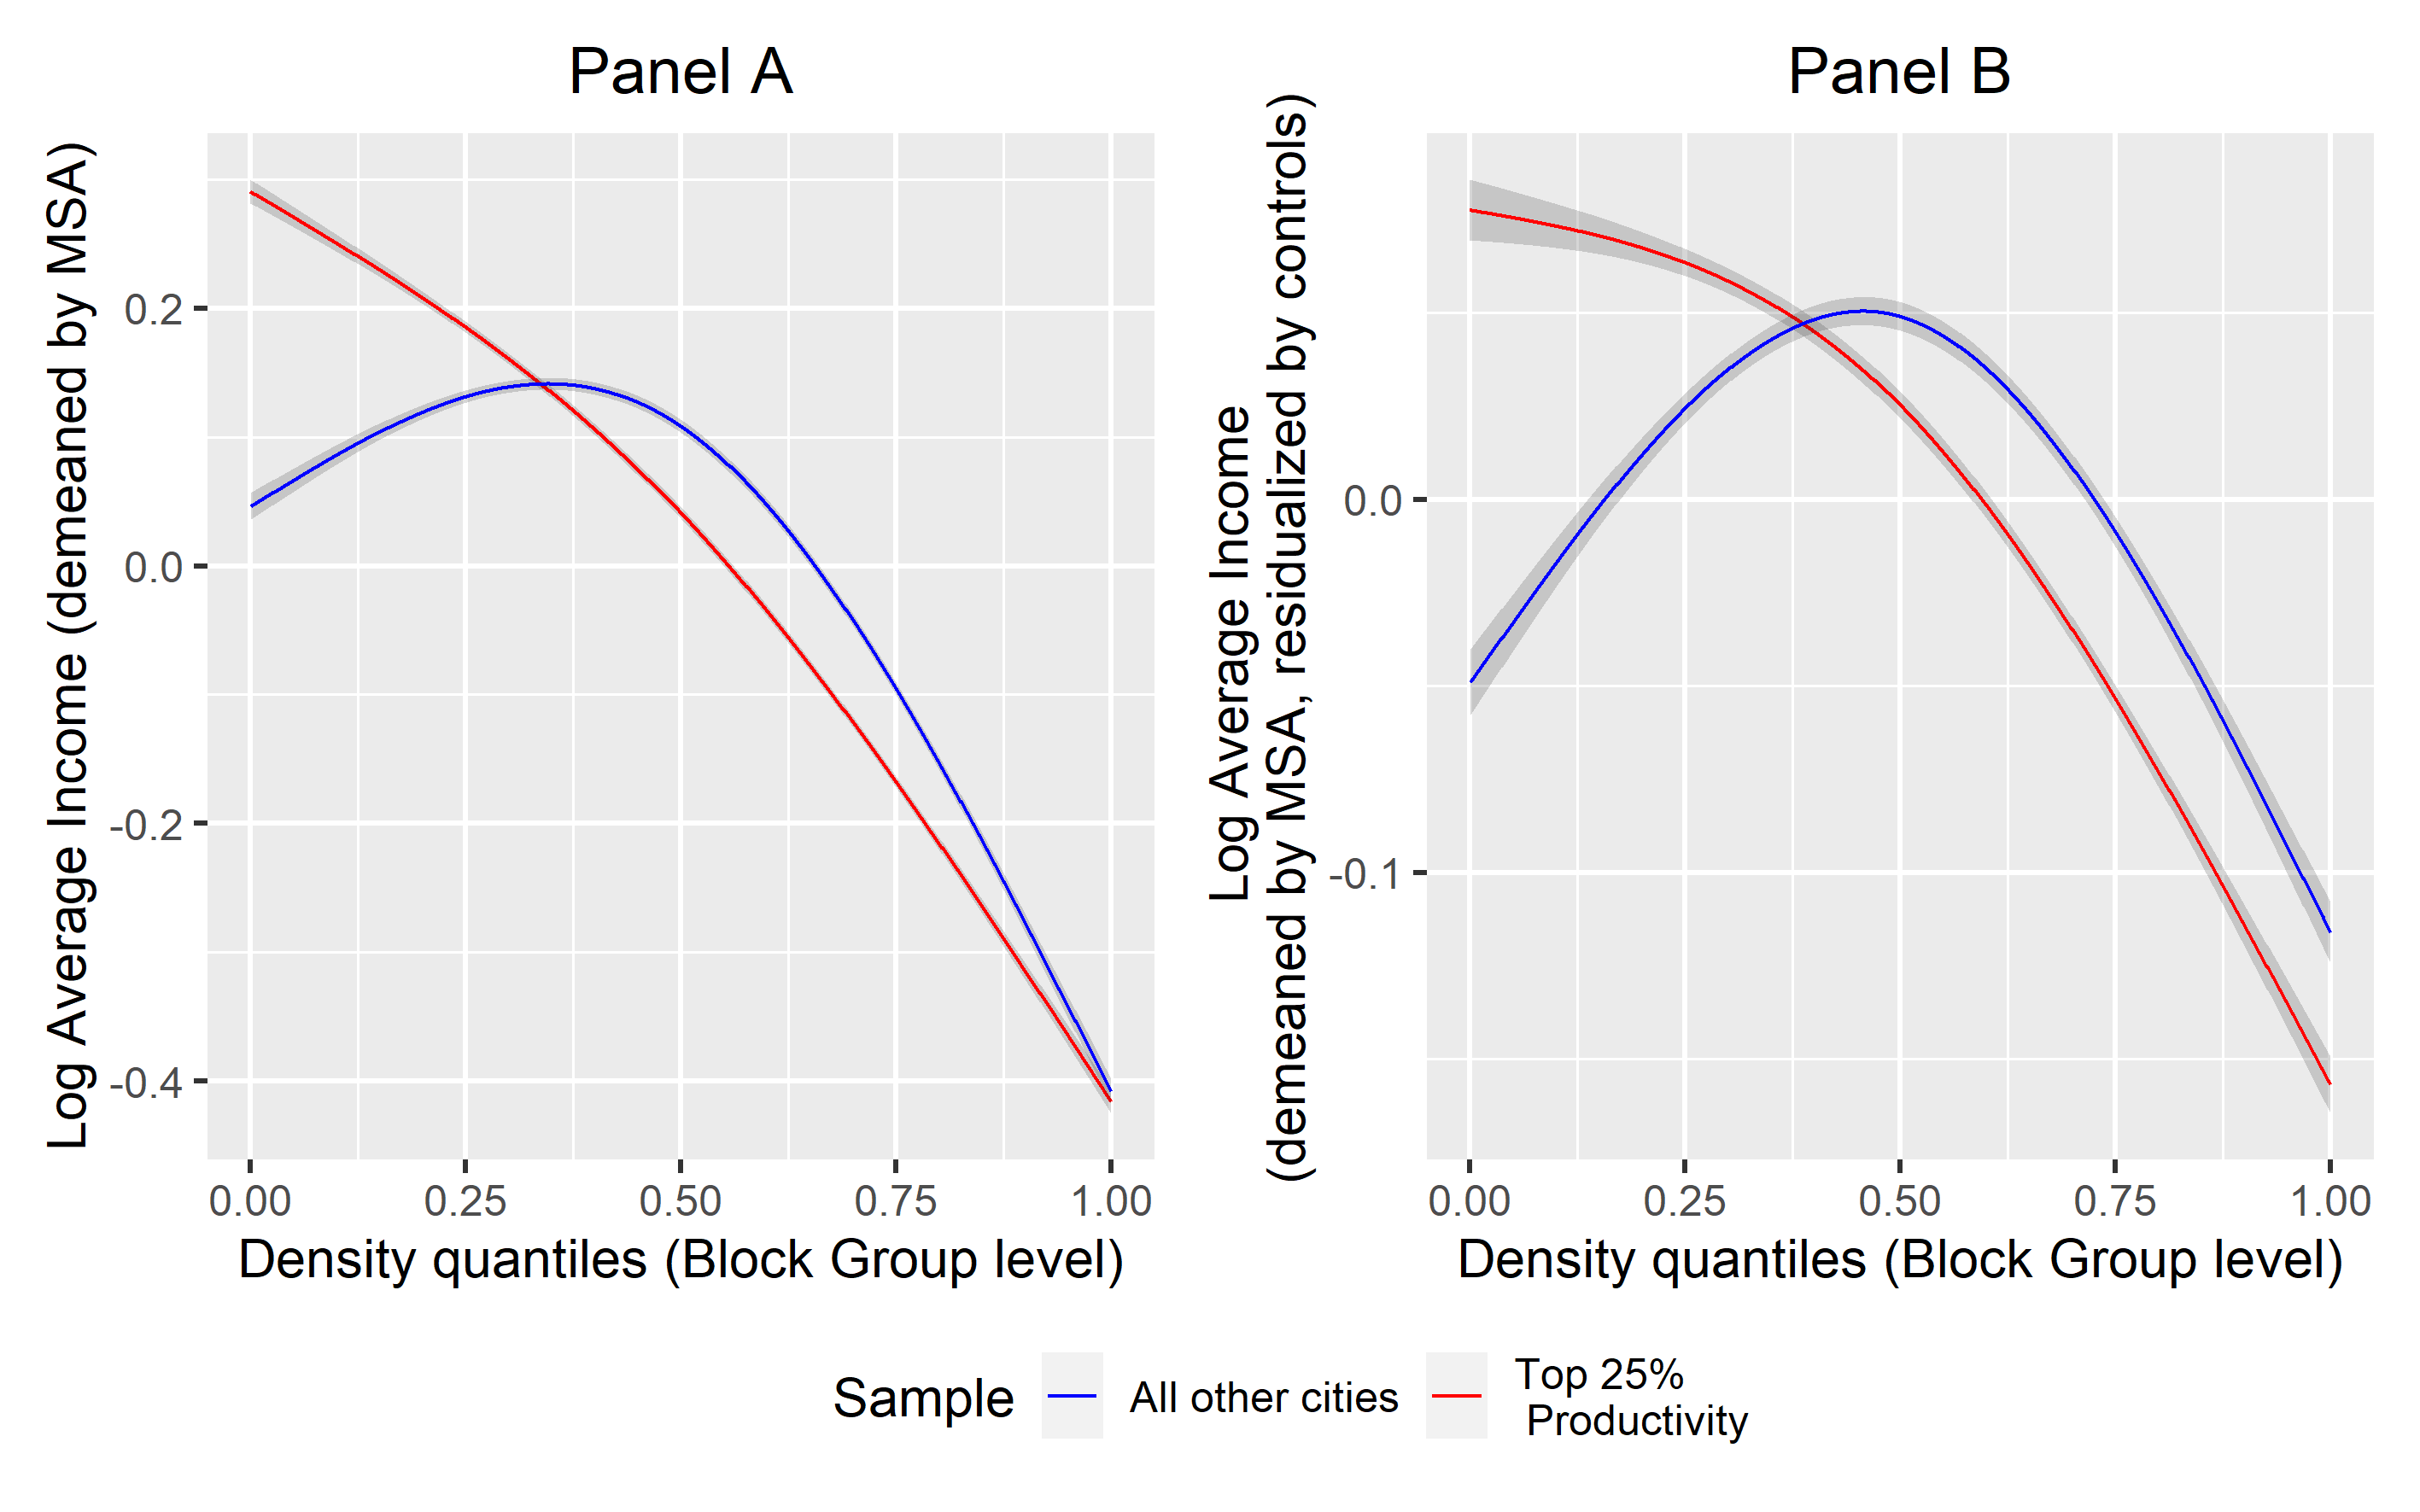
\includegraphics[width=\textwidth]{income_combined.png}
			\caption{ \\ Plot of cublic spline $\mathbf{S}$ from Equation \eqref{Specification:IncomeSortingStrong} with 5 knots, estimated with the \textit{mgcv} package in R \citep{gampackage}. 95\% confidence sets are reported. Panel A reports the model with  controls, while Panel B includes the model with the full set. The full set of controls are CBD distance, share of white households, building age, household size, share of households using public transport to commute, share of households using cars to commute, and average commuting time time from the ACS; density of performing arts, spectator sports, casinos, recreational activities, restaurants, fast food, bars and coffee shop establishments from NaNDA; and the density of EPA toxic releases and the density of public transport stops from NaNDA. All variables from the ACS vary at the block group level, and at the tract level for NaNDA.  }\label{Figure:IncomeSortingStrong}
		\end{center}
	\end{figure}
	
	\begin{figure}[htbp!]
		\begin{center}
			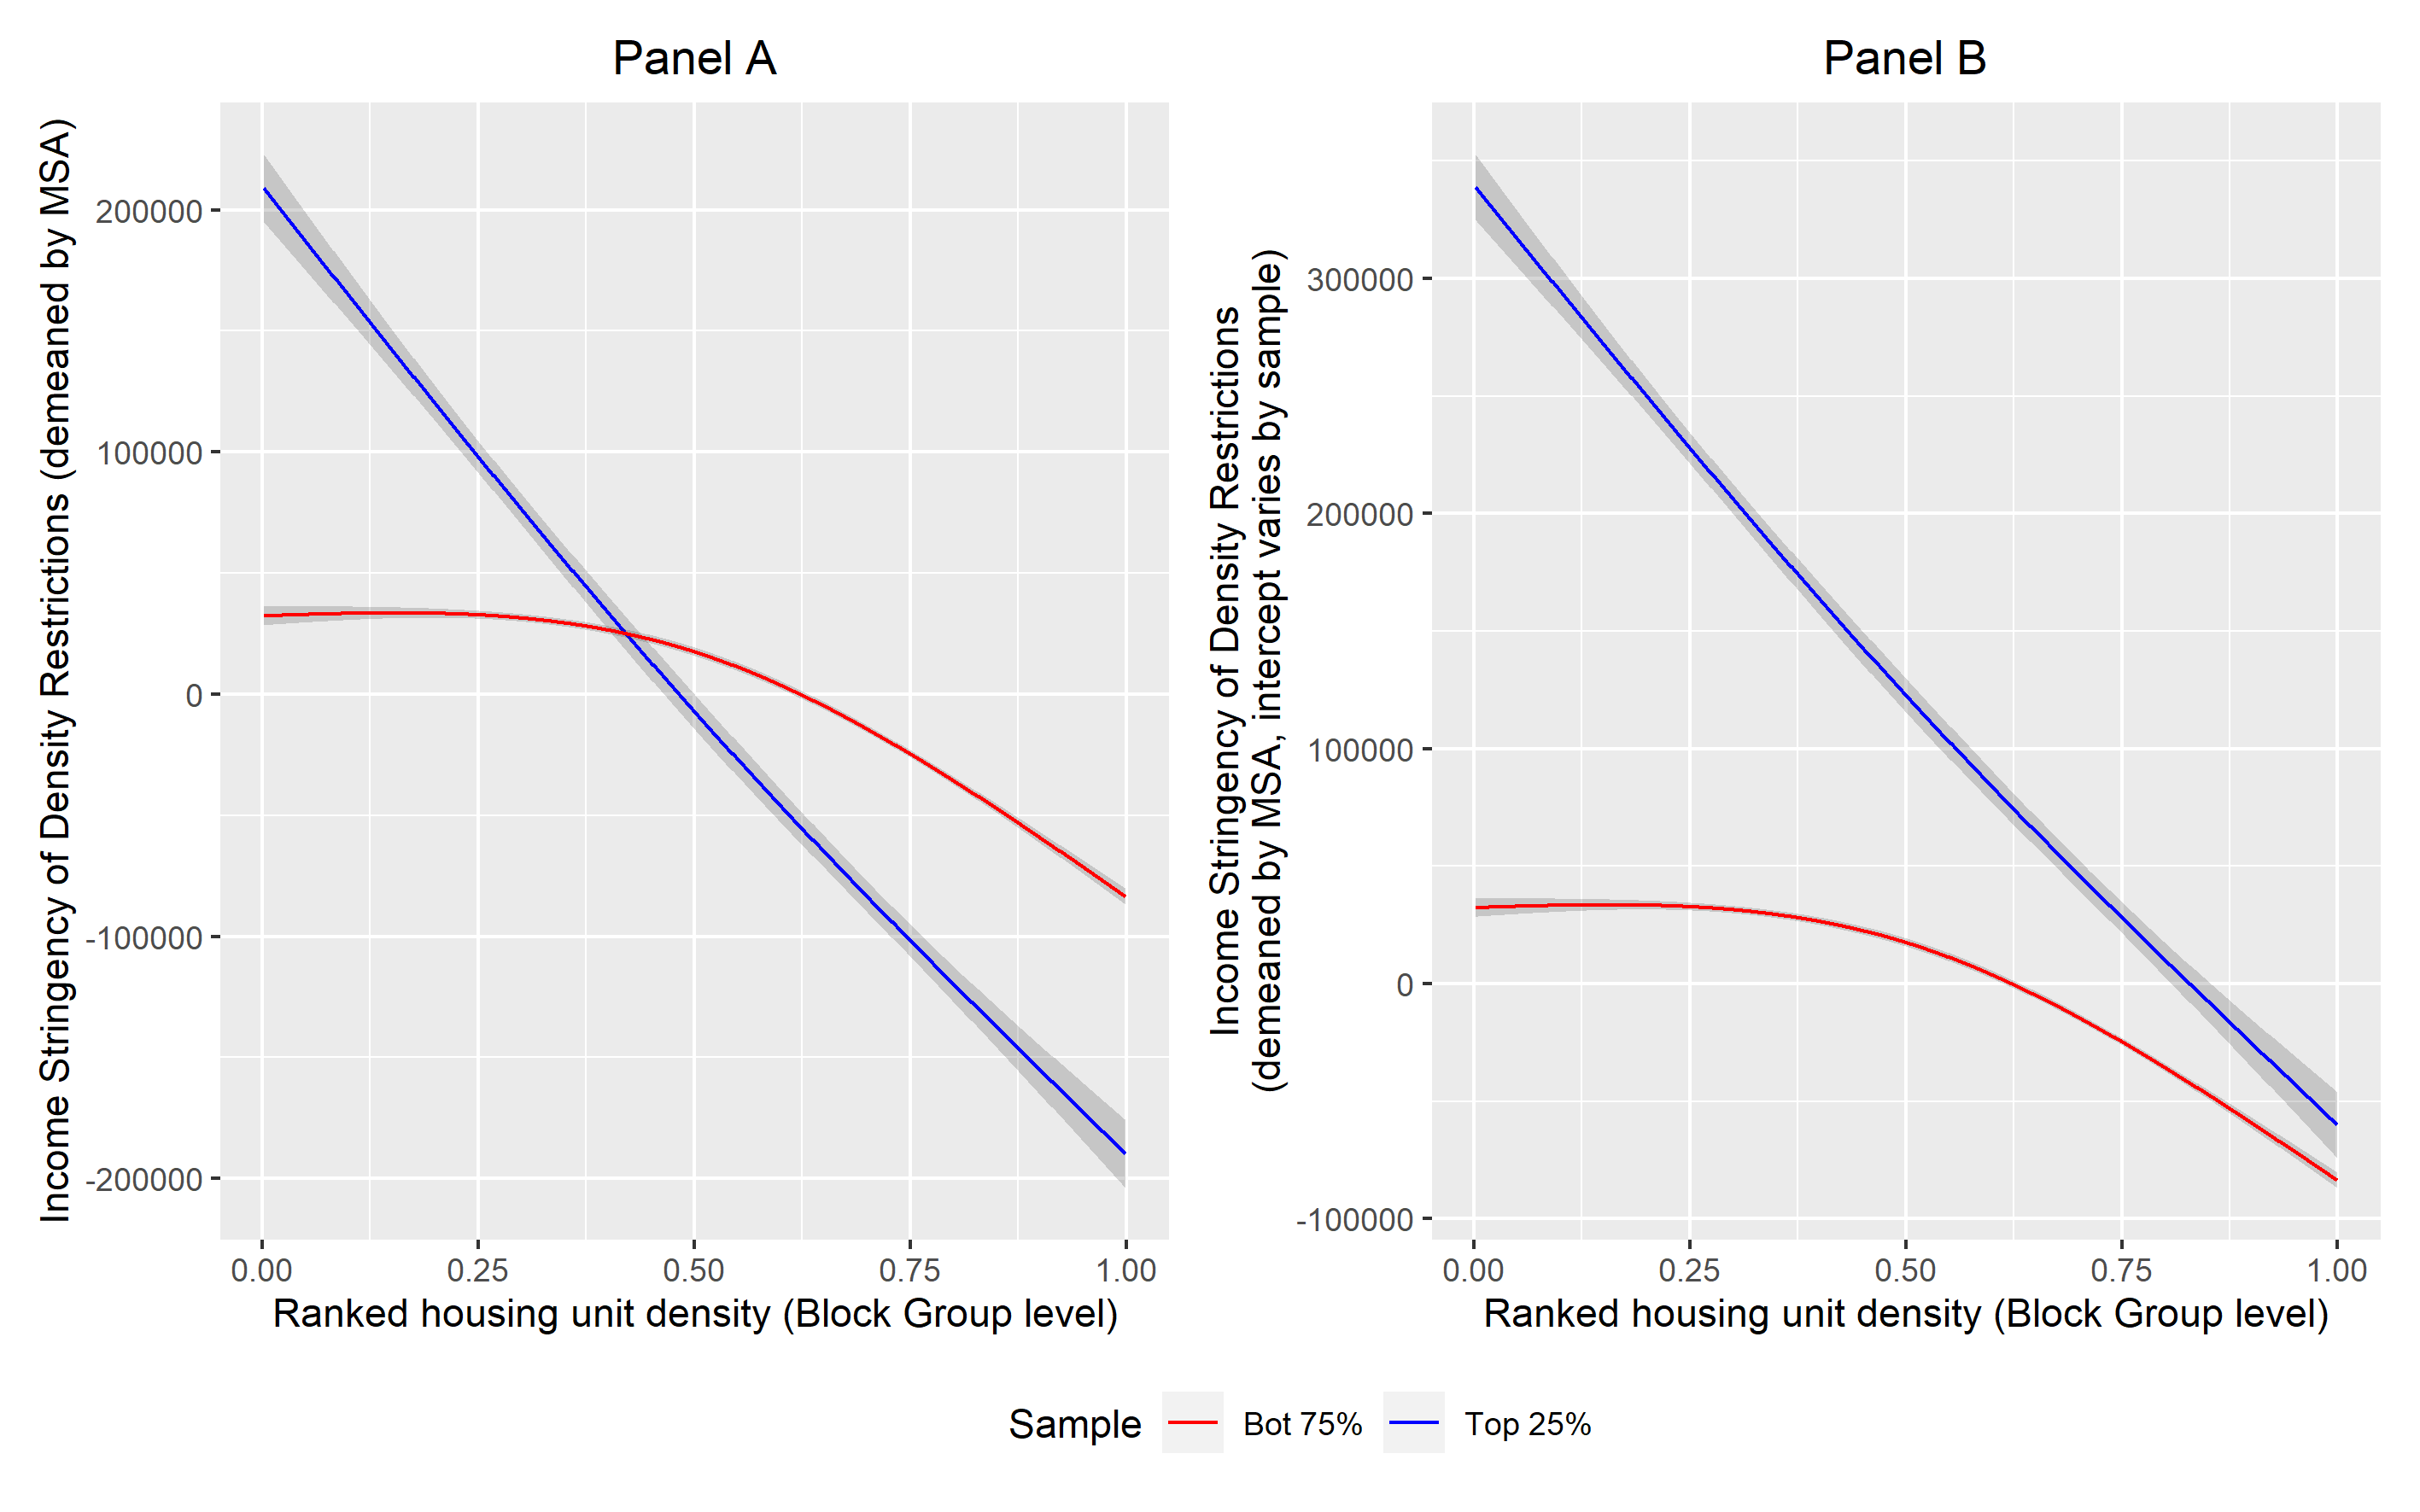
\includegraphics[width=\textwidth]{incomestringency_combined.png}
			\caption{\\ Plot of cublic spline $\mathbf{S}$ with 5 knots, estimated with the \textit{mgcv} package in R \citep{gampackage}. The specification in Panel A replaces log income in Equation \eqref{Specification:IncomeSortingStrong} with regulatory stringency in Equation \eqref{observedStringency} and \textit{excluded} controls, demeaned by city and measured in 2020 US dollars. The residualized version of this regression (mirroring Panel B of Figure \ref{Figure:IncomeSortingStrong}) is omitted as they look qualitatively identical under the same set of controls used in Figure \ref{Figure:IncomeSortingStrong}. 95 \% confidence sets are reported. Panel B repeats the same regression while allowing the average stringency to vary by sample. In other words, the blue curve is shifted upward by a constant. }\label{Figure:StringencyStrong} 
		\end{center}
	\end{figure}
	
	
	
	
	\begin{figure}[htbp!]
		\begin{center}
		\caption{ \\ Equivalent variation for deregulation by household type. }\label{figure:welfare_ctfl}
			\makebox[\textwidth]{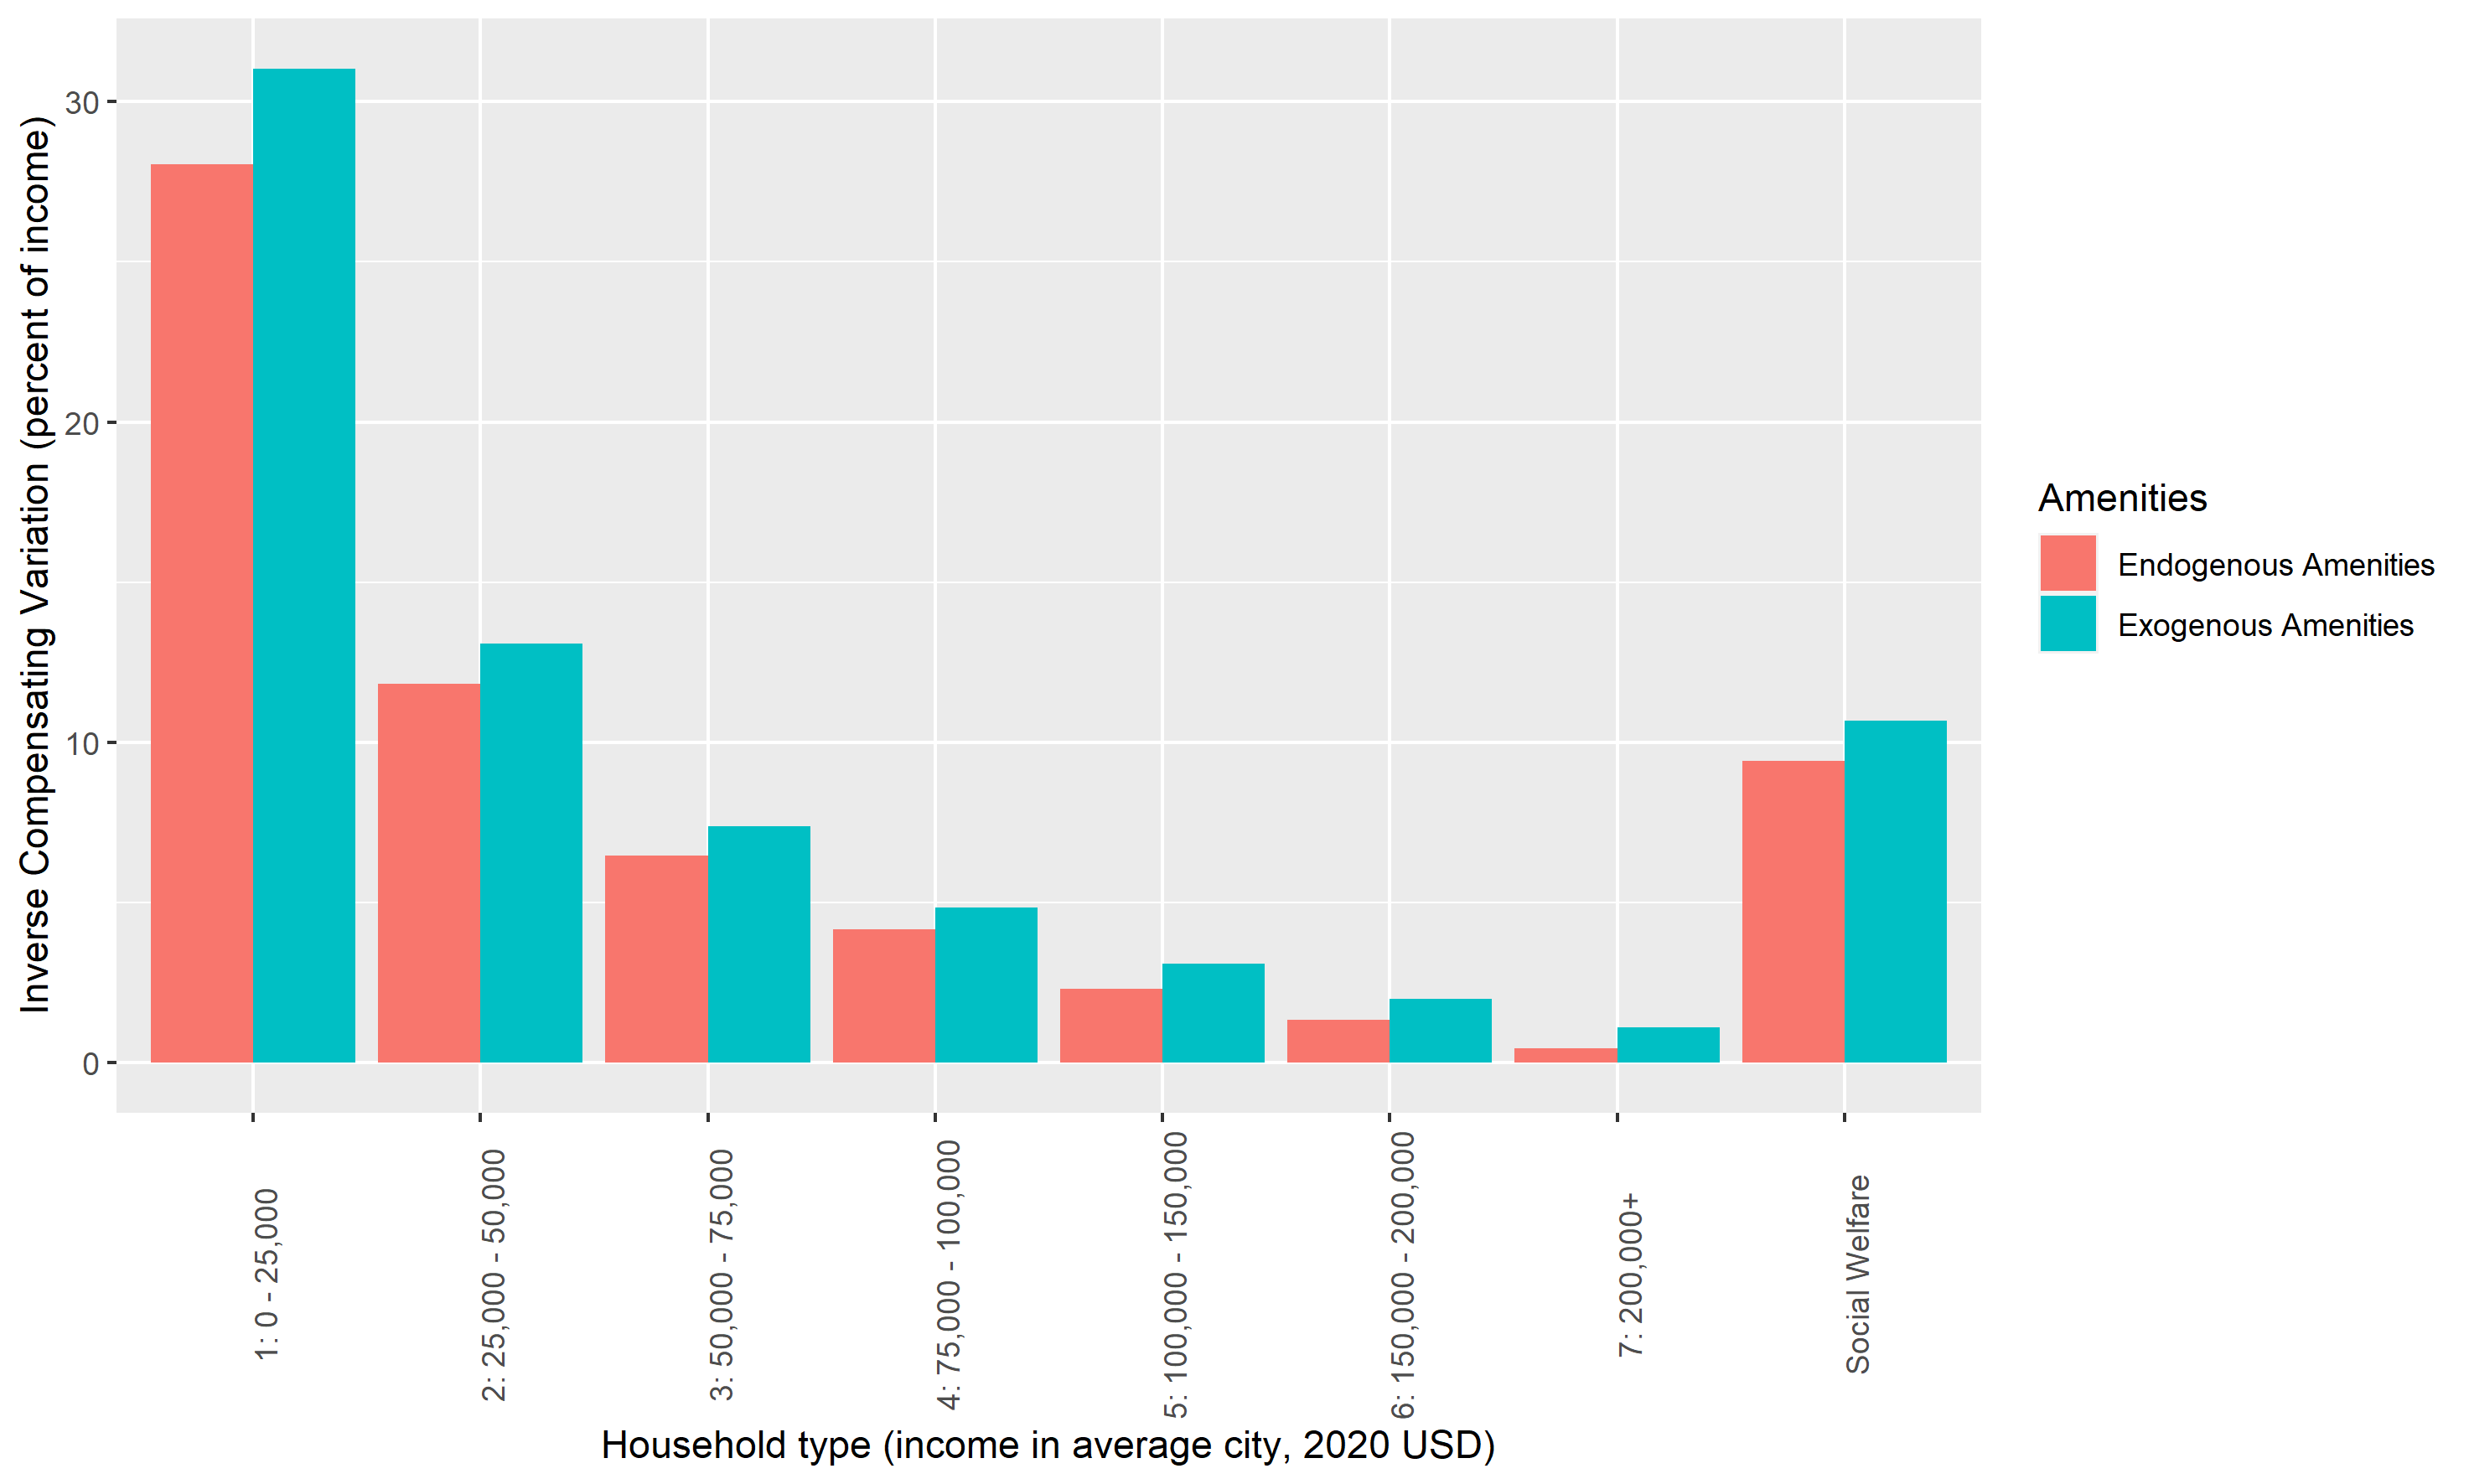
\includegraphics[width=1.1\textwidth]{Welfare.png}}
		\end{center}
		\caption*{Welfare is measured as the equivalent variation and expressed as a percentage of baseline income. Higher values mean higher welfare gains. Social welfare is the population weighted average of welfare by type. "Endogenous Amenities" refers to counterfactual outcomes under the baseline model. "Exogenous" refers to counterfactuals under the parameter restriction $\Omega(z) = 0$ for all $z$.}
	\end{figure}
	
	
	
	
	\begin{figure}[htbp!]
		\begin{center}
			\caption{ \\ Equivalent variation for deregulation by household type, \\ pooled over renters and homeowners and including capital losses. }\label{figure:welfarePooled_ctfl}
			\makebox[\textwidth]{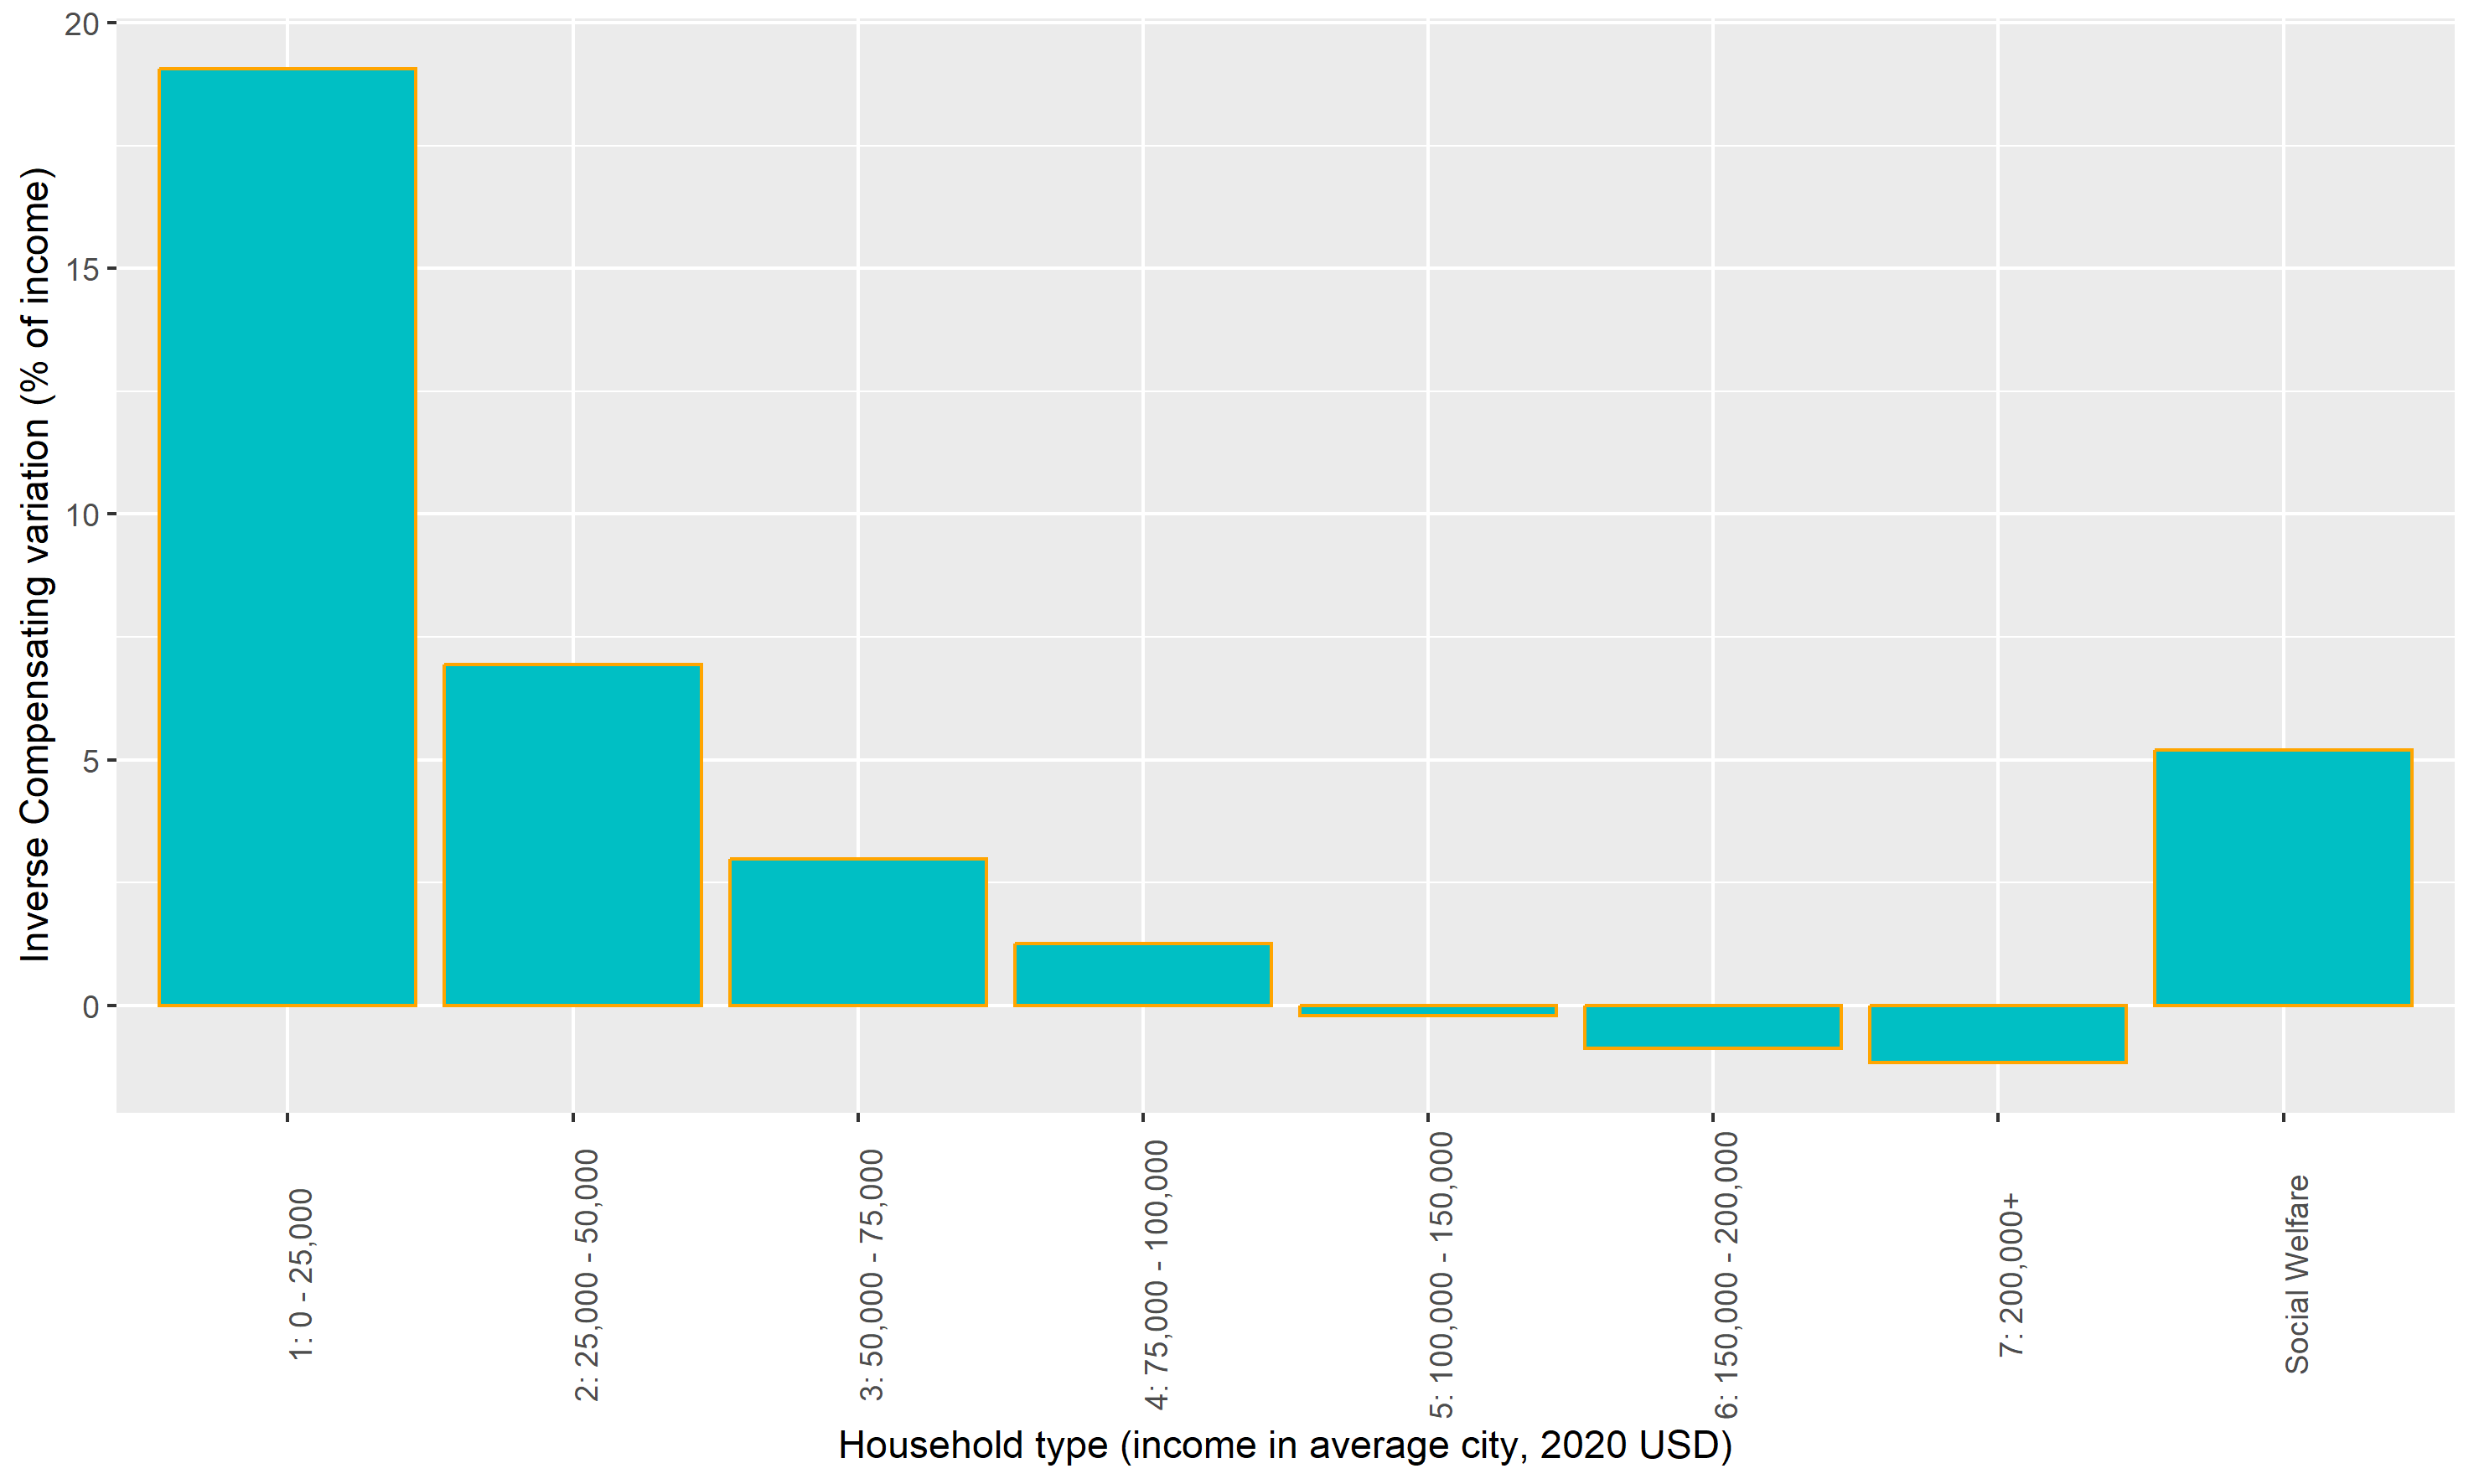
\includegraphics[width=\textwidth]{WelfarePooled.png}}
		\end{center}
		\caption*{Welfare is measured as the equivalent variation and expressed as a percentage of initial income. Higher values mean higher welfare gains. Social welfare is the population weighted average of welfare by type. Results incorporate capital losses for homeowners by income type, using a procedure outlined in Appendix \ref{Appendix:RenterLandownerWelfare}. Results include equilibrium adjustments to neighborhood amenity value as in the baseline counterfactual. Renters and homeowners are pooled by type using a population-weighted average of welfare changes.}
	\end{figure}
	
	
	
	\begin{figure}[htbp!]
		\begin{center}
			\caption{ \\ Shapely decomposition of welfare into consumption and amenities}\label{figure:welfareDecomp_ctfl}
			\makebox[\textwidth]{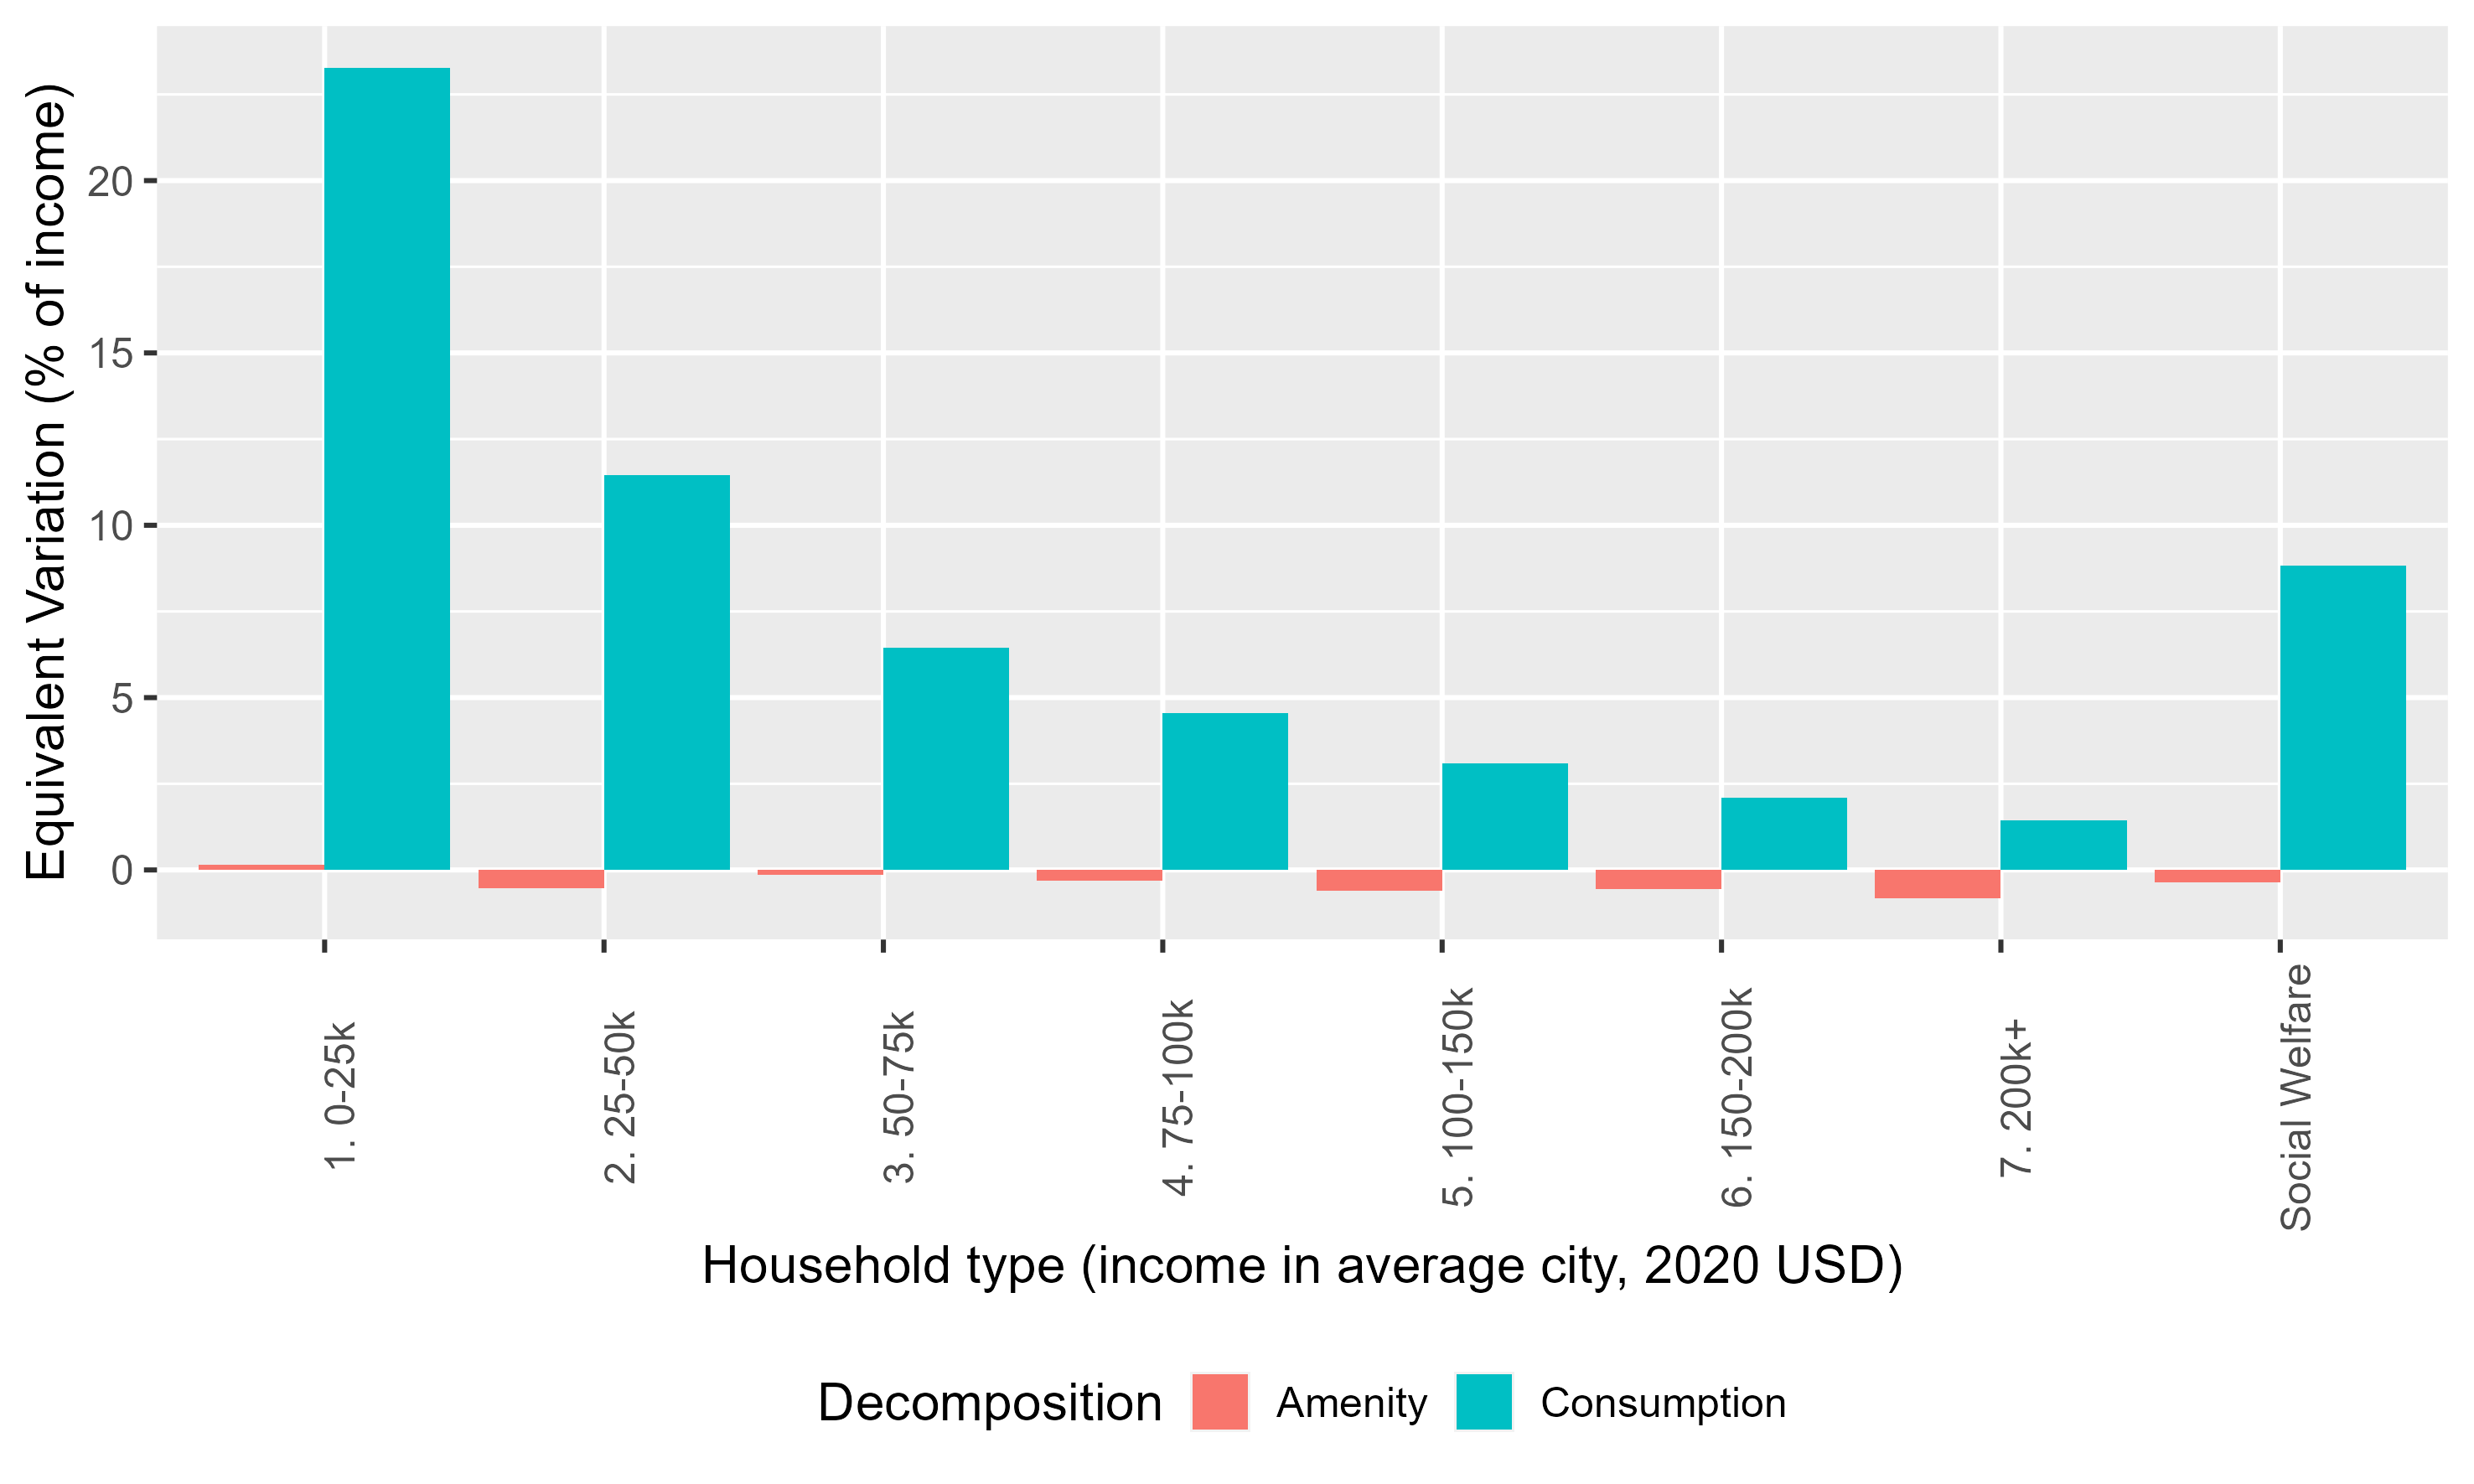
\includegraphics[width=\textwidth]{WelfareDecomp.png}}
		\end{center}
		\caption*{Welfare is measured as the equivalent variation as a percentage of baseline income. Higher values mean higher welfare gains. Social welfare is the population weighted average of welfare by type. "Amenity" and "Consumption" components are constructed using Shapely values, with a procedure outlined in Appendix \ref{Appendix:ShapeDecompDefn}. The sum of components add to the equivalent variation reported in Figure \ref{figure:welfare_ctfl}. }
	\end{figure}
	
	
	
	\begin{figure}[htbp!]
			\caption{ \\ Shapely decomposition of welfare into consumption and amenities, \\
					fundamental amenities are equal across income types}\label{figure:welfareDecompNoFund_ctfl}
					
			\makebox[\textwidth]{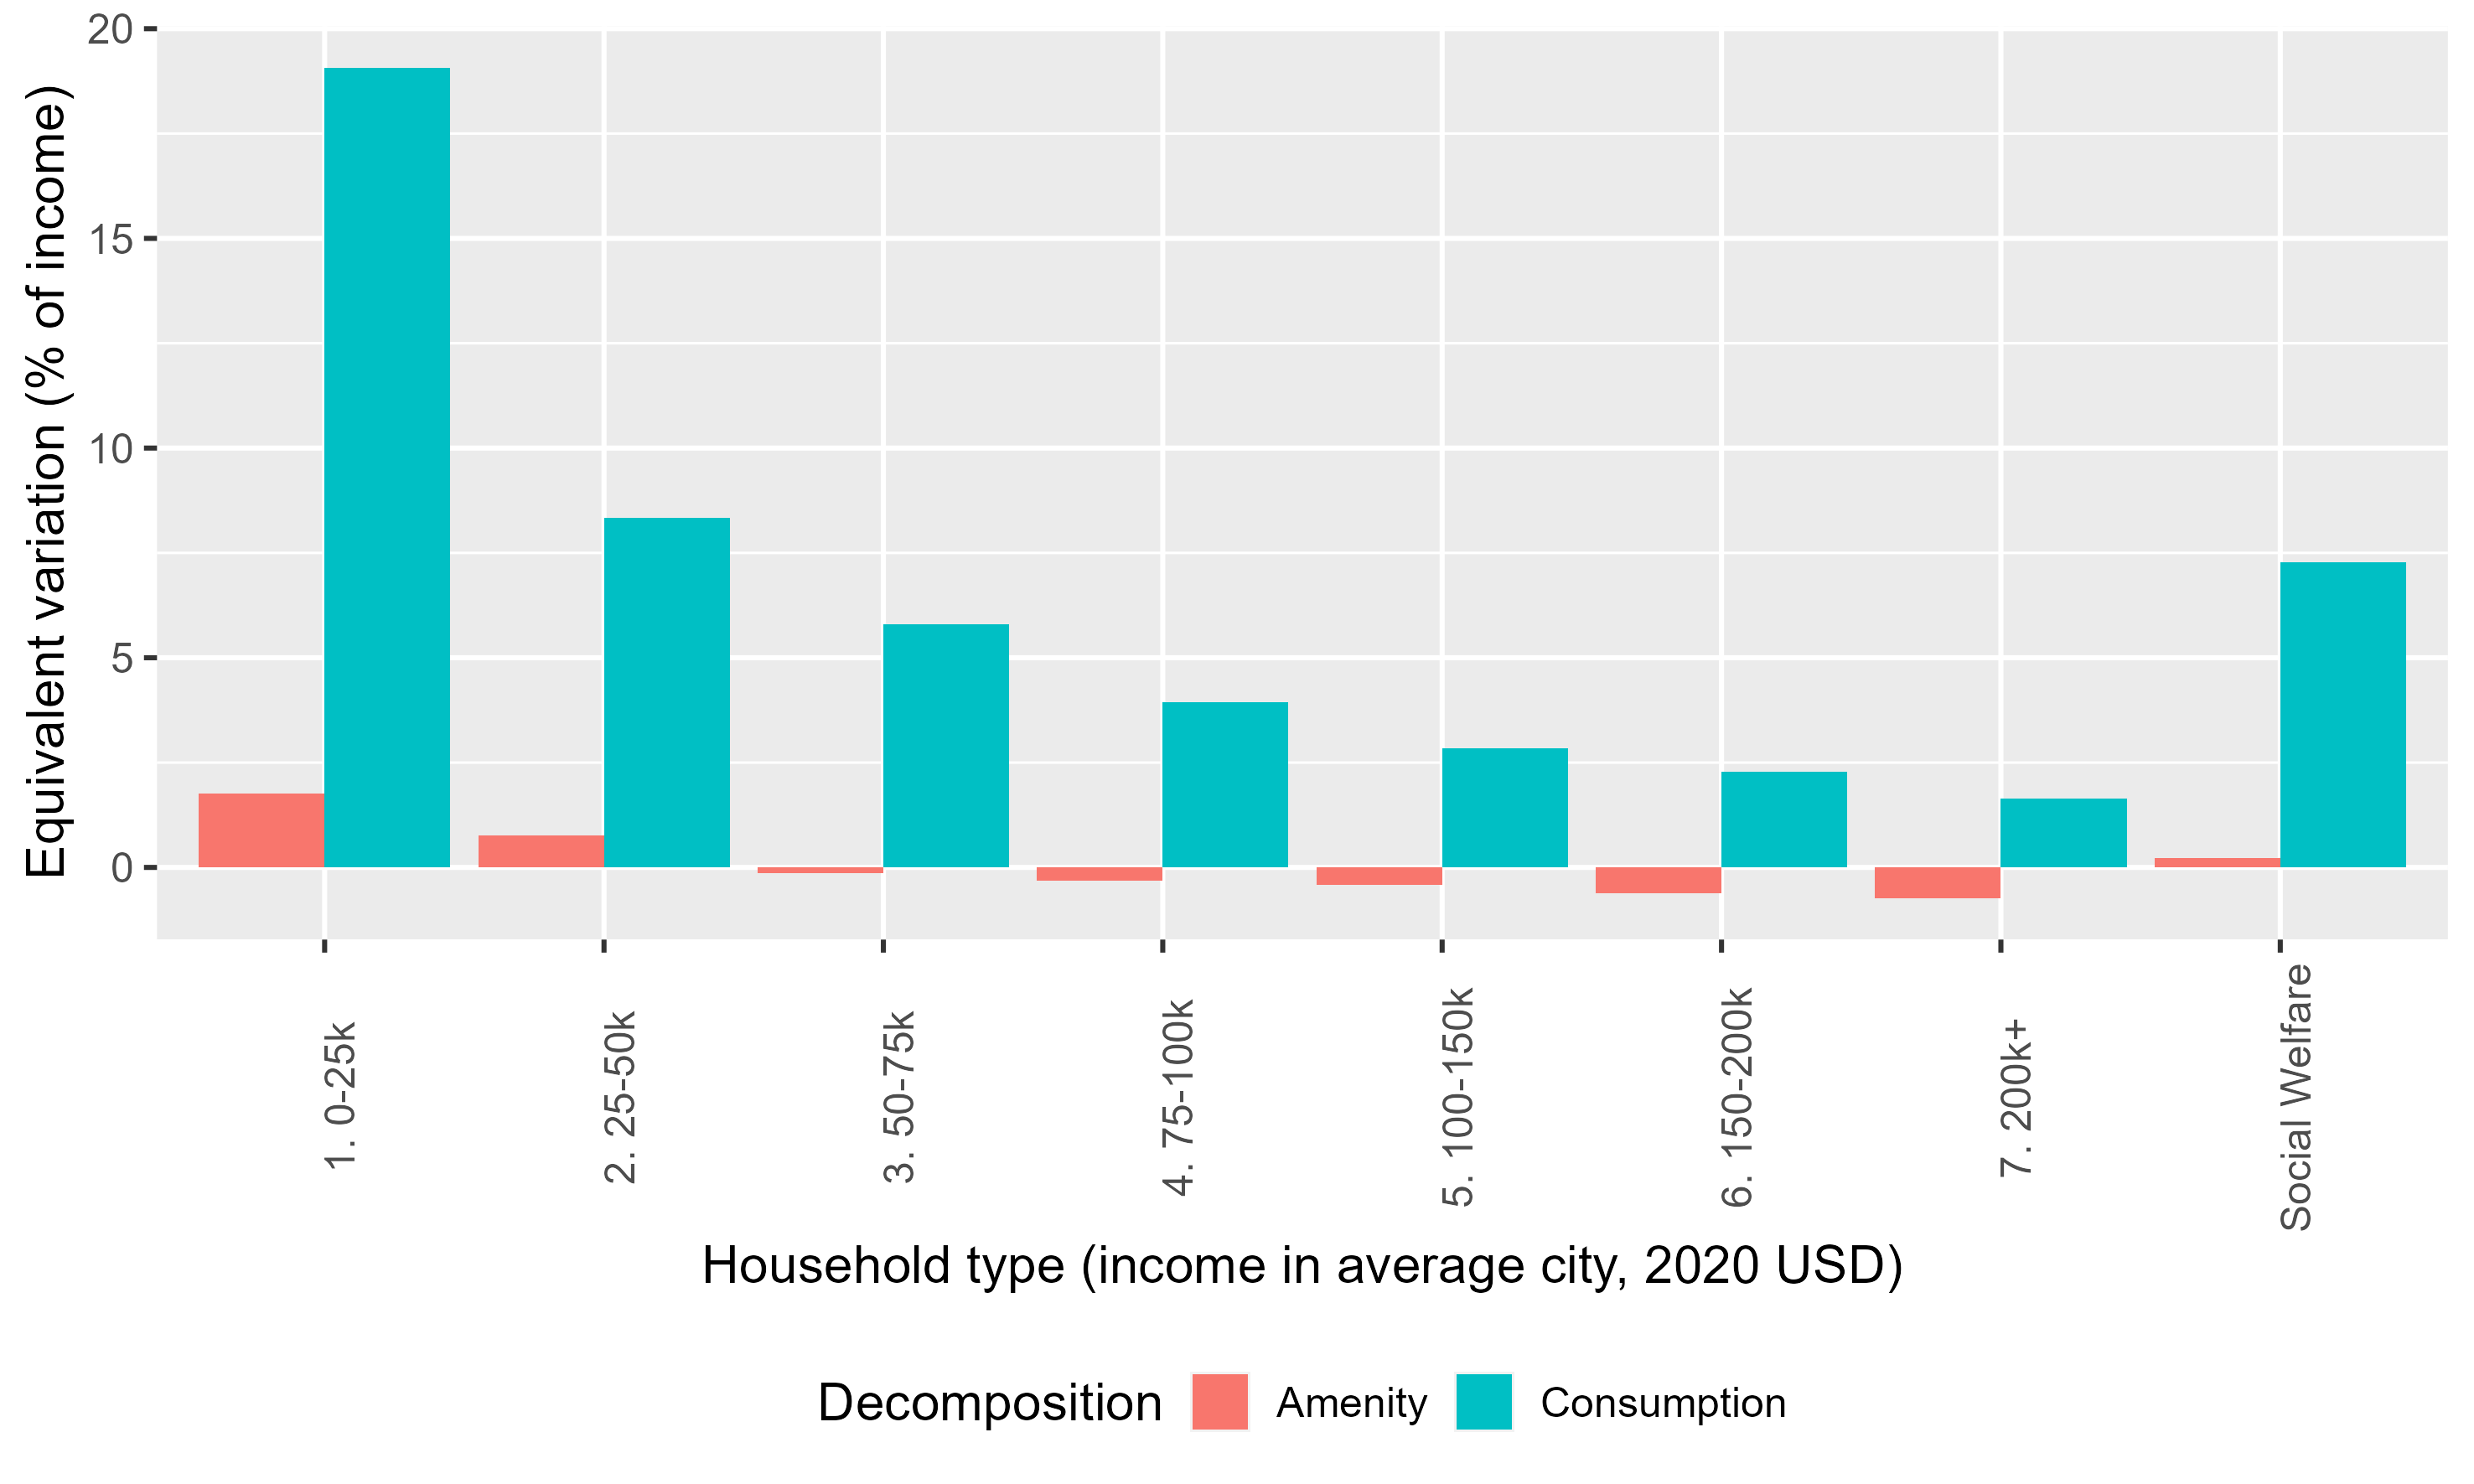
\includegraphics[width=\textwidth]{WelfareDecompNoFund.png}}
				\caption*{Welfare is measured as the equivalent variation as a percentage of baseline income. Higher values mean higher welfare gains. Social welfare is the population weighted average of welfare by type. "Amenity" and "Consumption" components are constructed using Shapely values, with a procedure outlined in Appendix \ref{Appendix:ShapeDecompDefn}. The sum of components add to the equivalent variation associated with full deregulation with no fundamental amenity differences across different income types.}
		
	\end{figure}
	
	
	
	
	\begin{figure}[htbp!]
		
		\caption{ \\ Gentrification in superstar cities post deregulation.}\label{figure:gentrification}
		\makebox[\textwidth]{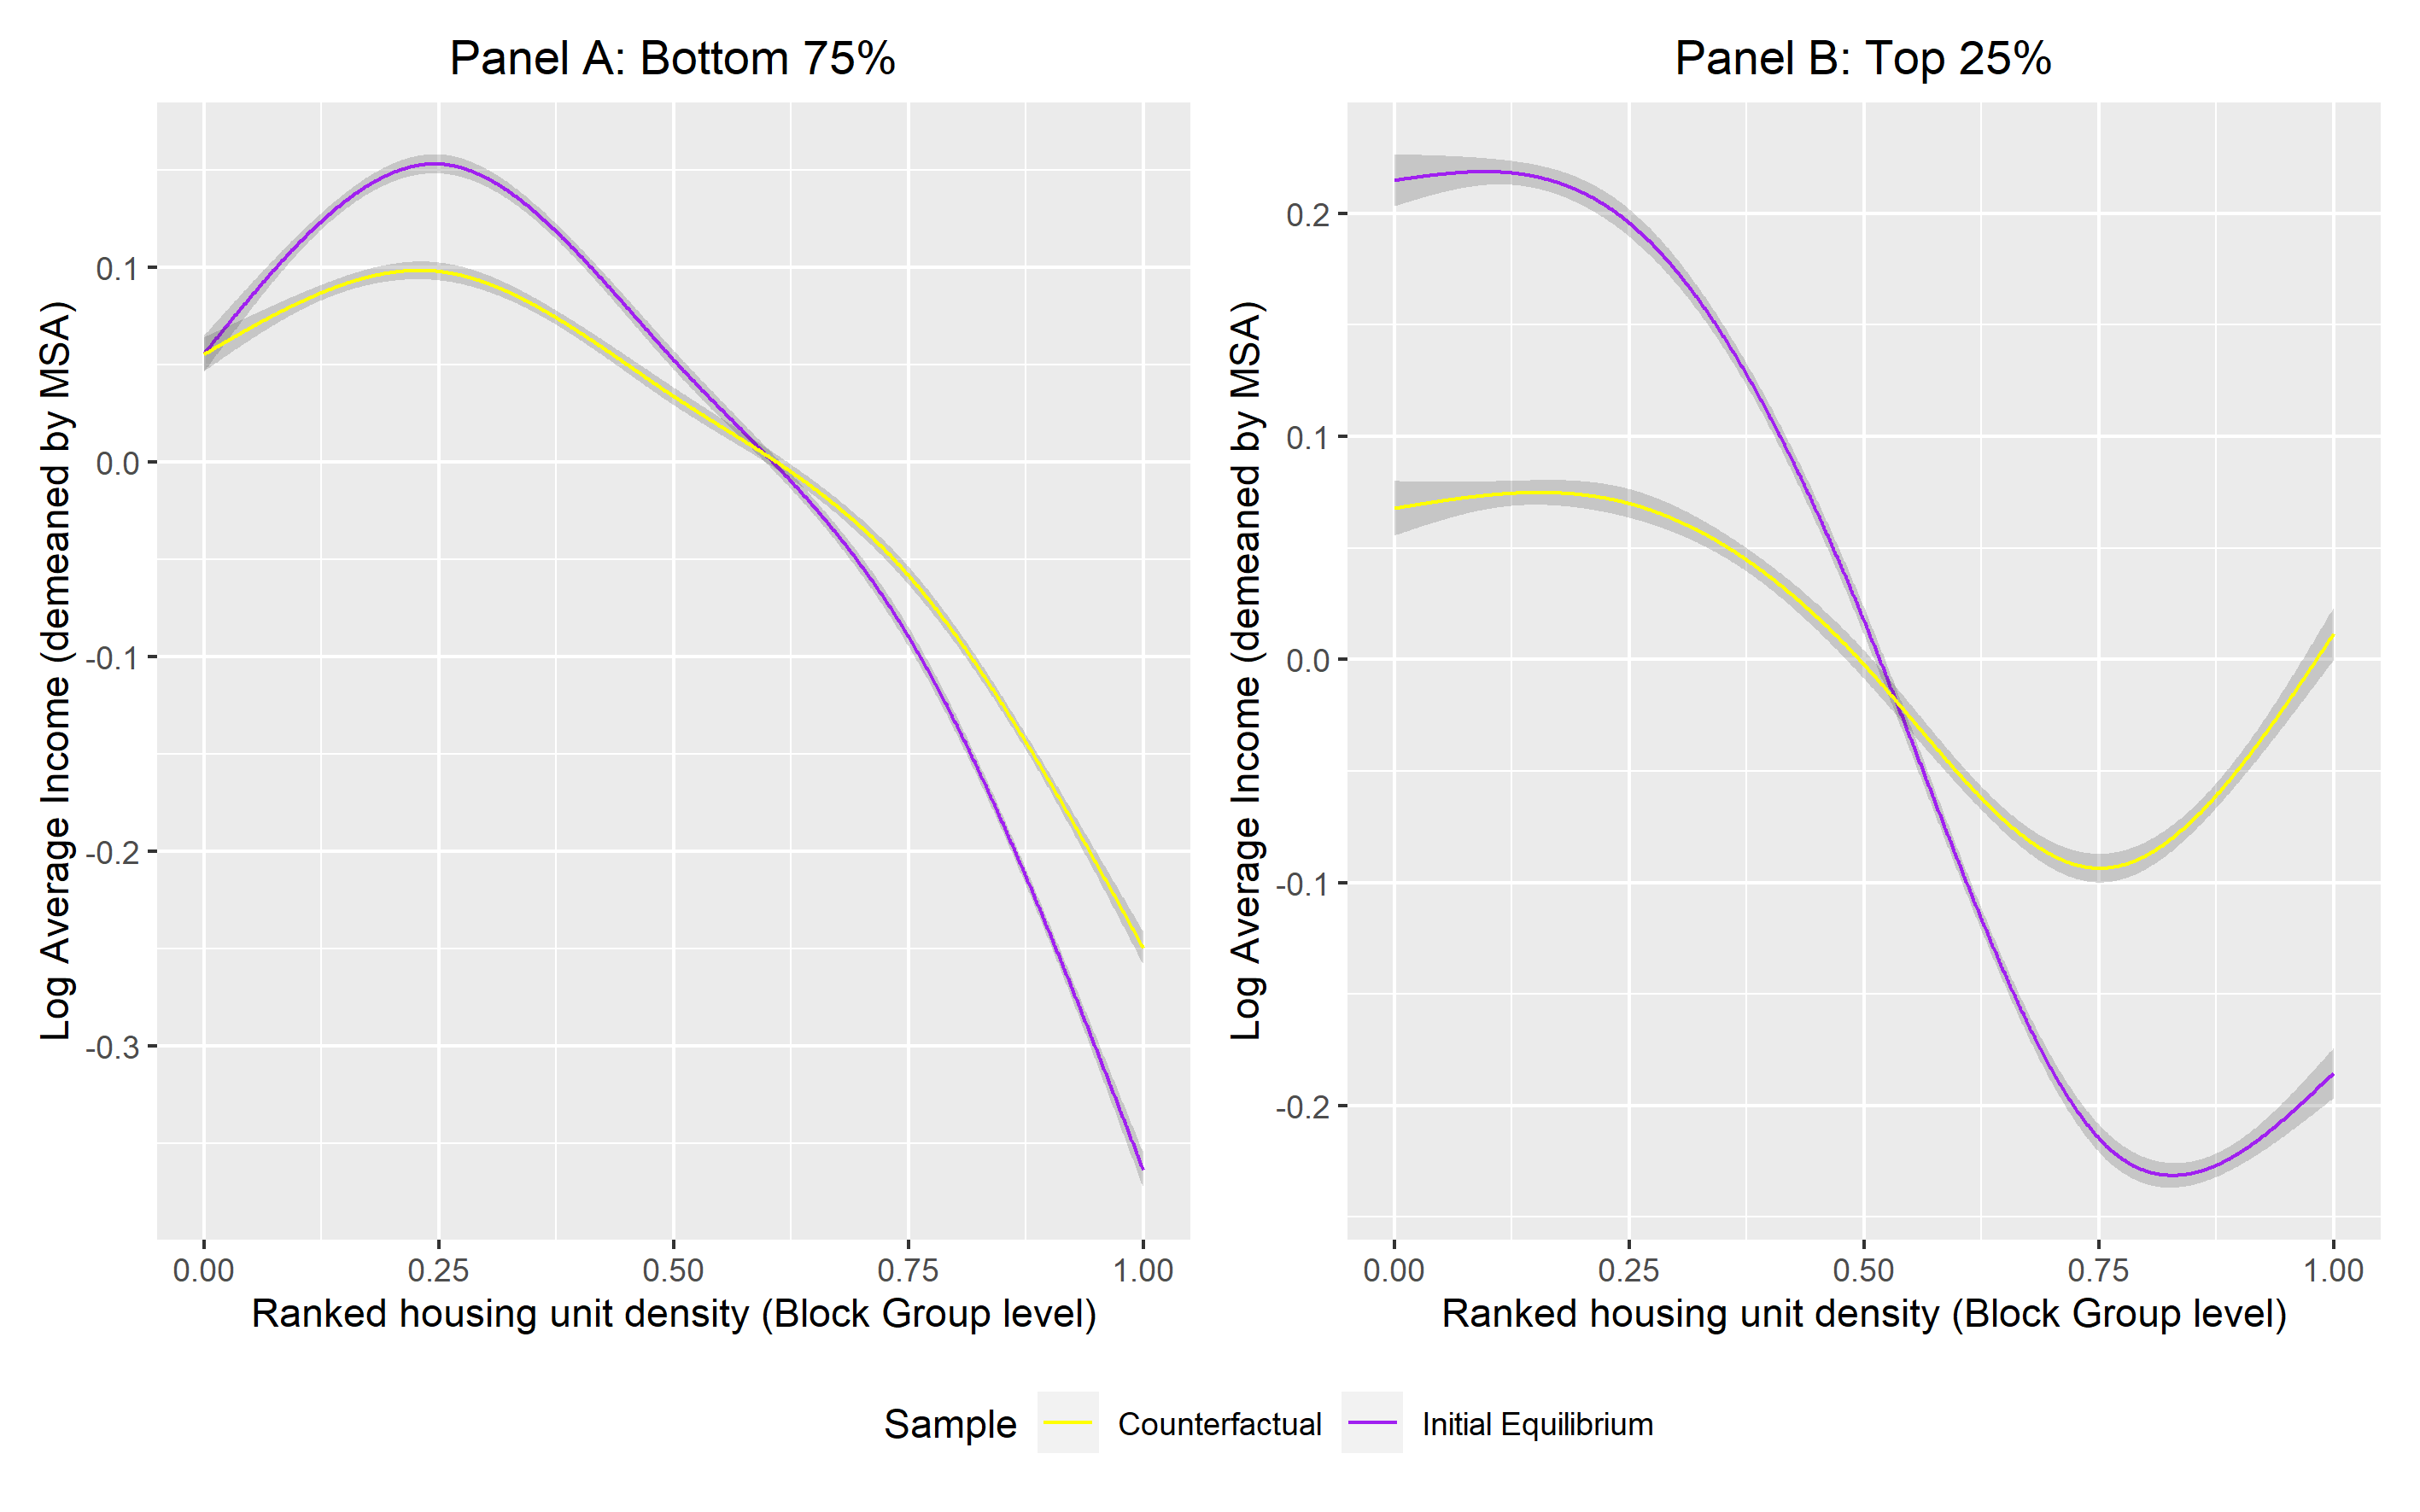
\includegraphics[width=\textwidth]{IncomeDensityGradCtfl.png}}
		
		\caption*{For each panel, demeaned log average income at the neighborhood level is regressed against the observed density ranking of neighborhoods at baseline. The purple regression uses data from the baseline equilibrium that matches data, as in Figure \ref{FIncomeDens}. The yellow regression uses data generated from the counterfactual with no minimum lot sizes. Each panel corresponds to "superstar" sample cities (Top $25 \%$) and "non-superstar" sample cities (Bottom $75 \%$), as in Figure \ref{FIncomeDens}. }
		
	\end{figure}
	
	
	\begin{landscape}
	\begin{figure}[htbp!]
		\begin{center}
		\caption{City income sorting.}\label{figure:city_inc_sorting}
		\makebox{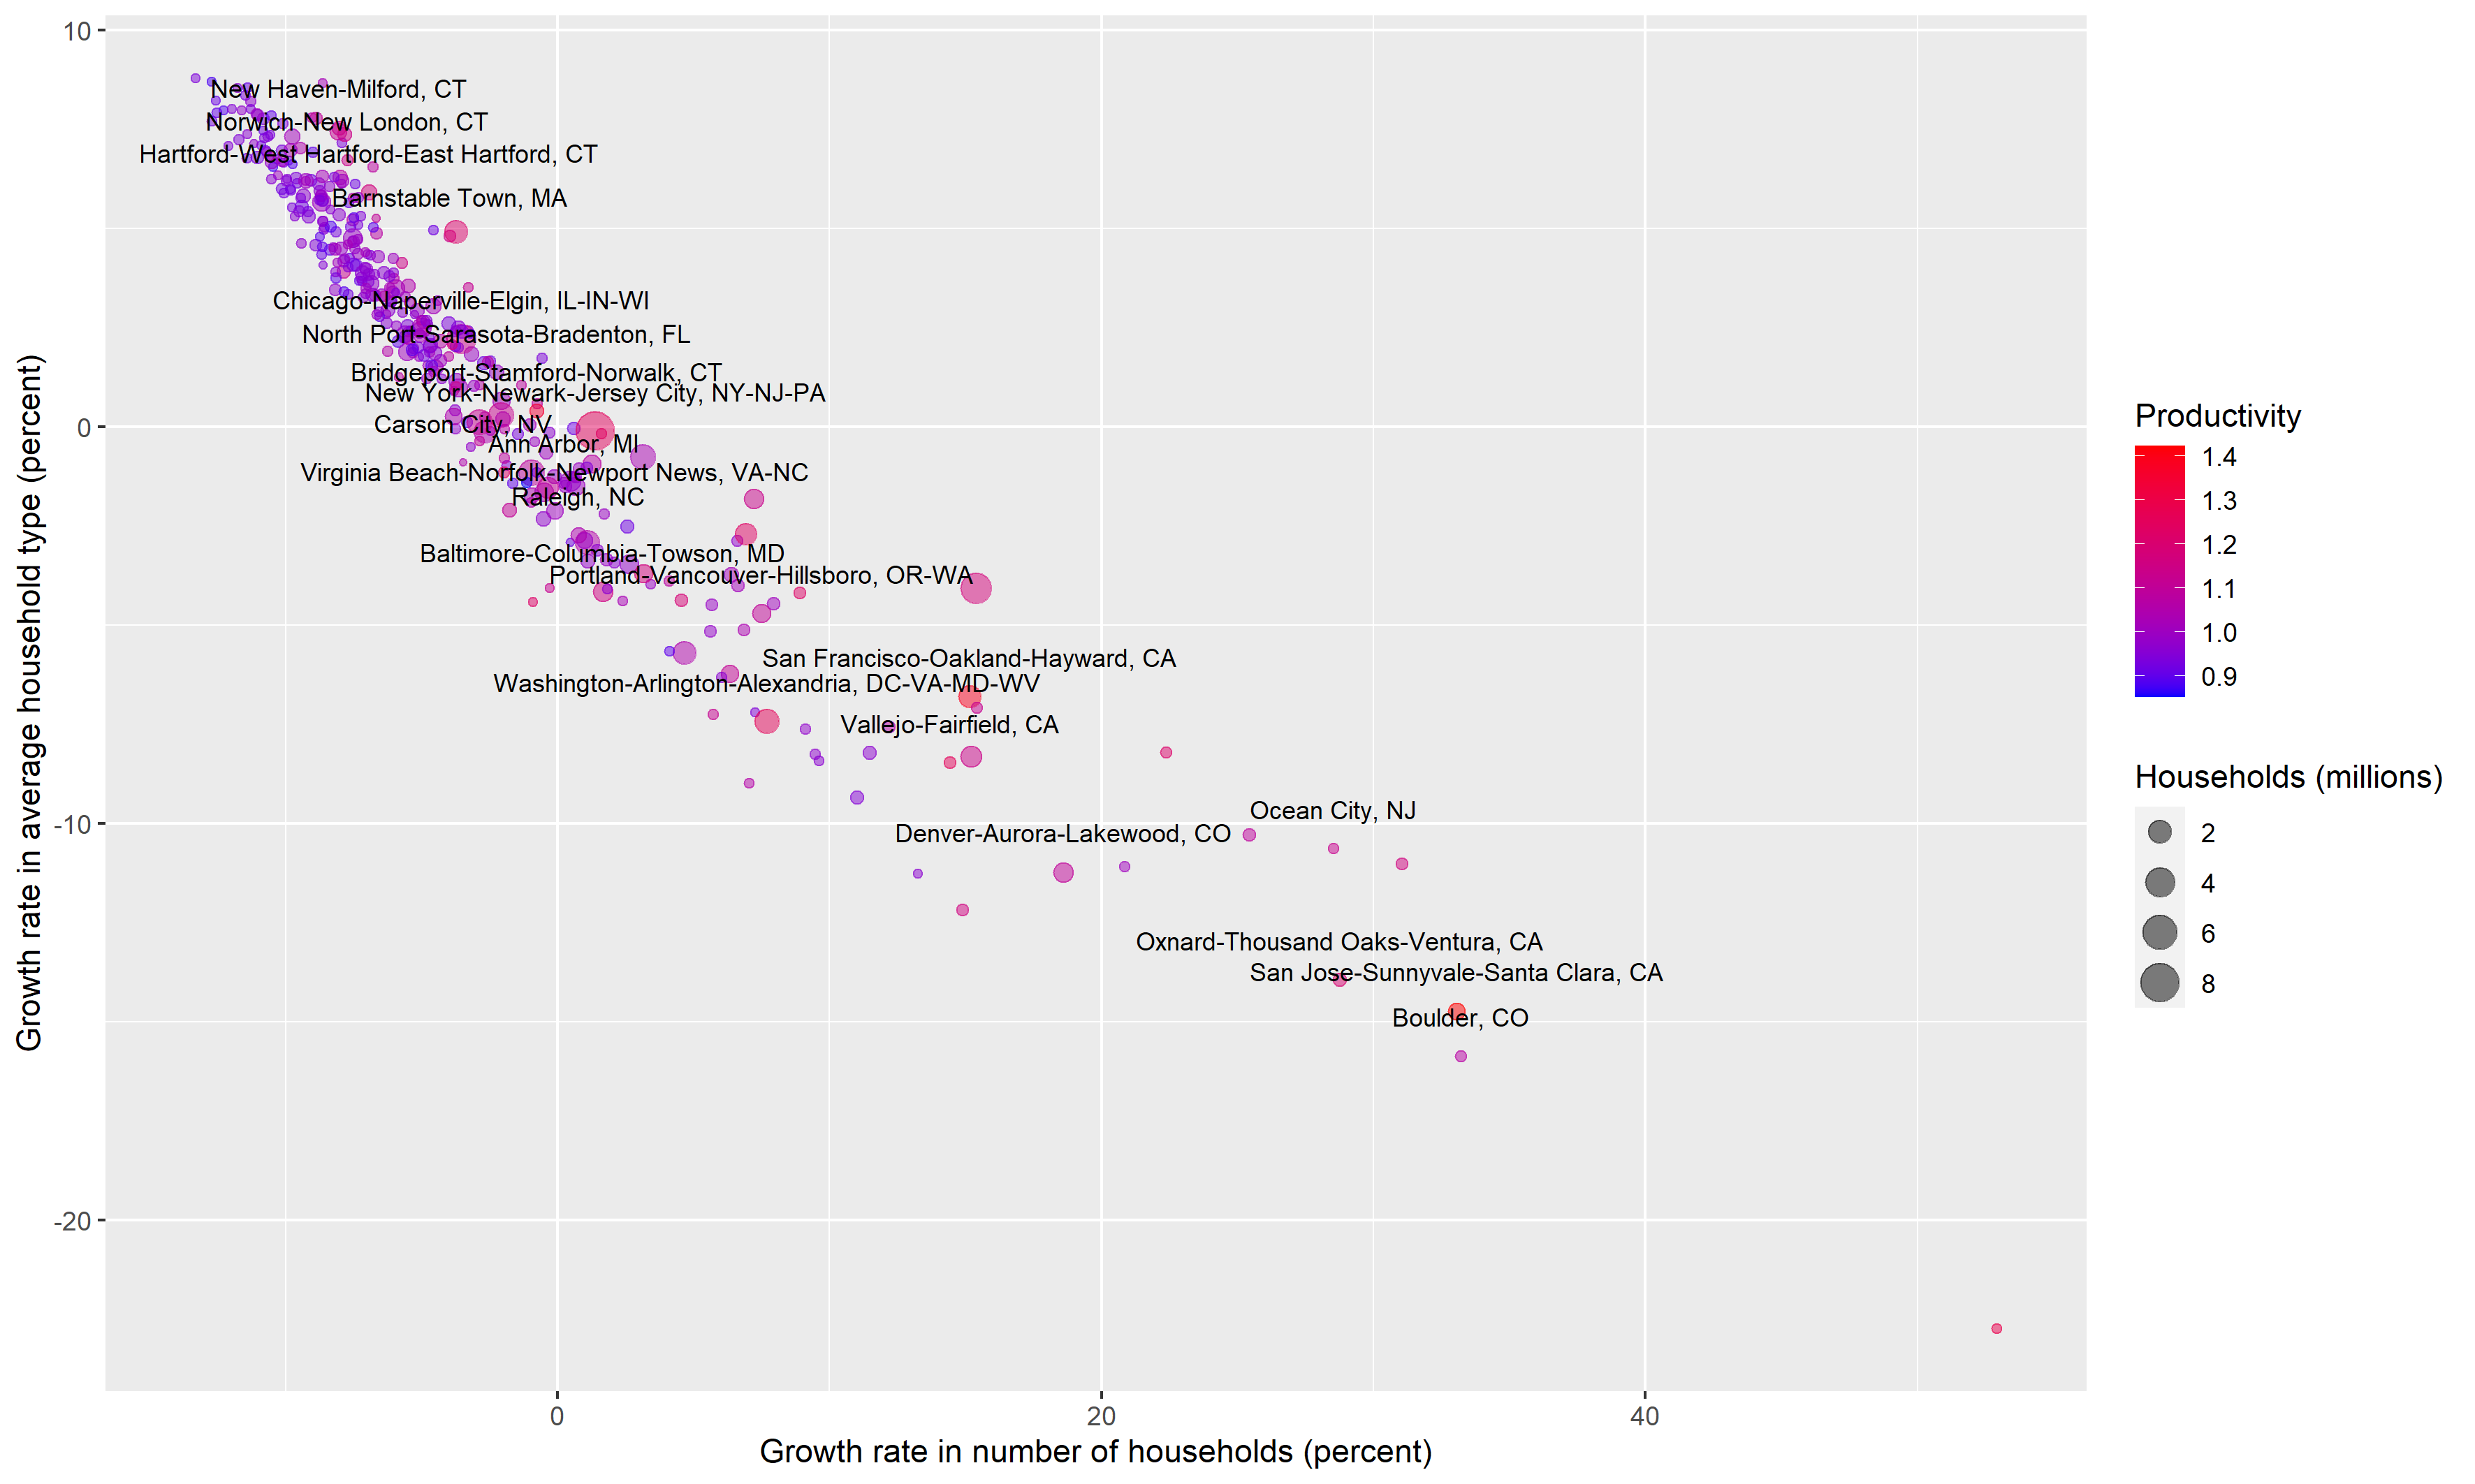
\includegraphics[width = 0.9\linewidth, height = \textheight]{IncomeSortingMovement.png}}
		
		\caption*{The $y$ axis is defined as the change in the average income that a household could earn in an average city from baseline to counterfactual. Correlation between the growth rate in the number of households productivity is approximately $50\%$, and this correlation is $70\%$ for unadjusted housing prices.  Cities on the top left (high income, negative population growth) tend to have low productivity, and cities with higher productivity tend to be in the bottom left.}
		\end{center}
	\end{figure}
	\end{landscape}
	
	
	\begin{figure}[htbp!]
		
		\caption{Changes in land values by regulatory stringency in the baseline equilibrium.}\label{figure:landlords}
		\makebox[\textwidth]{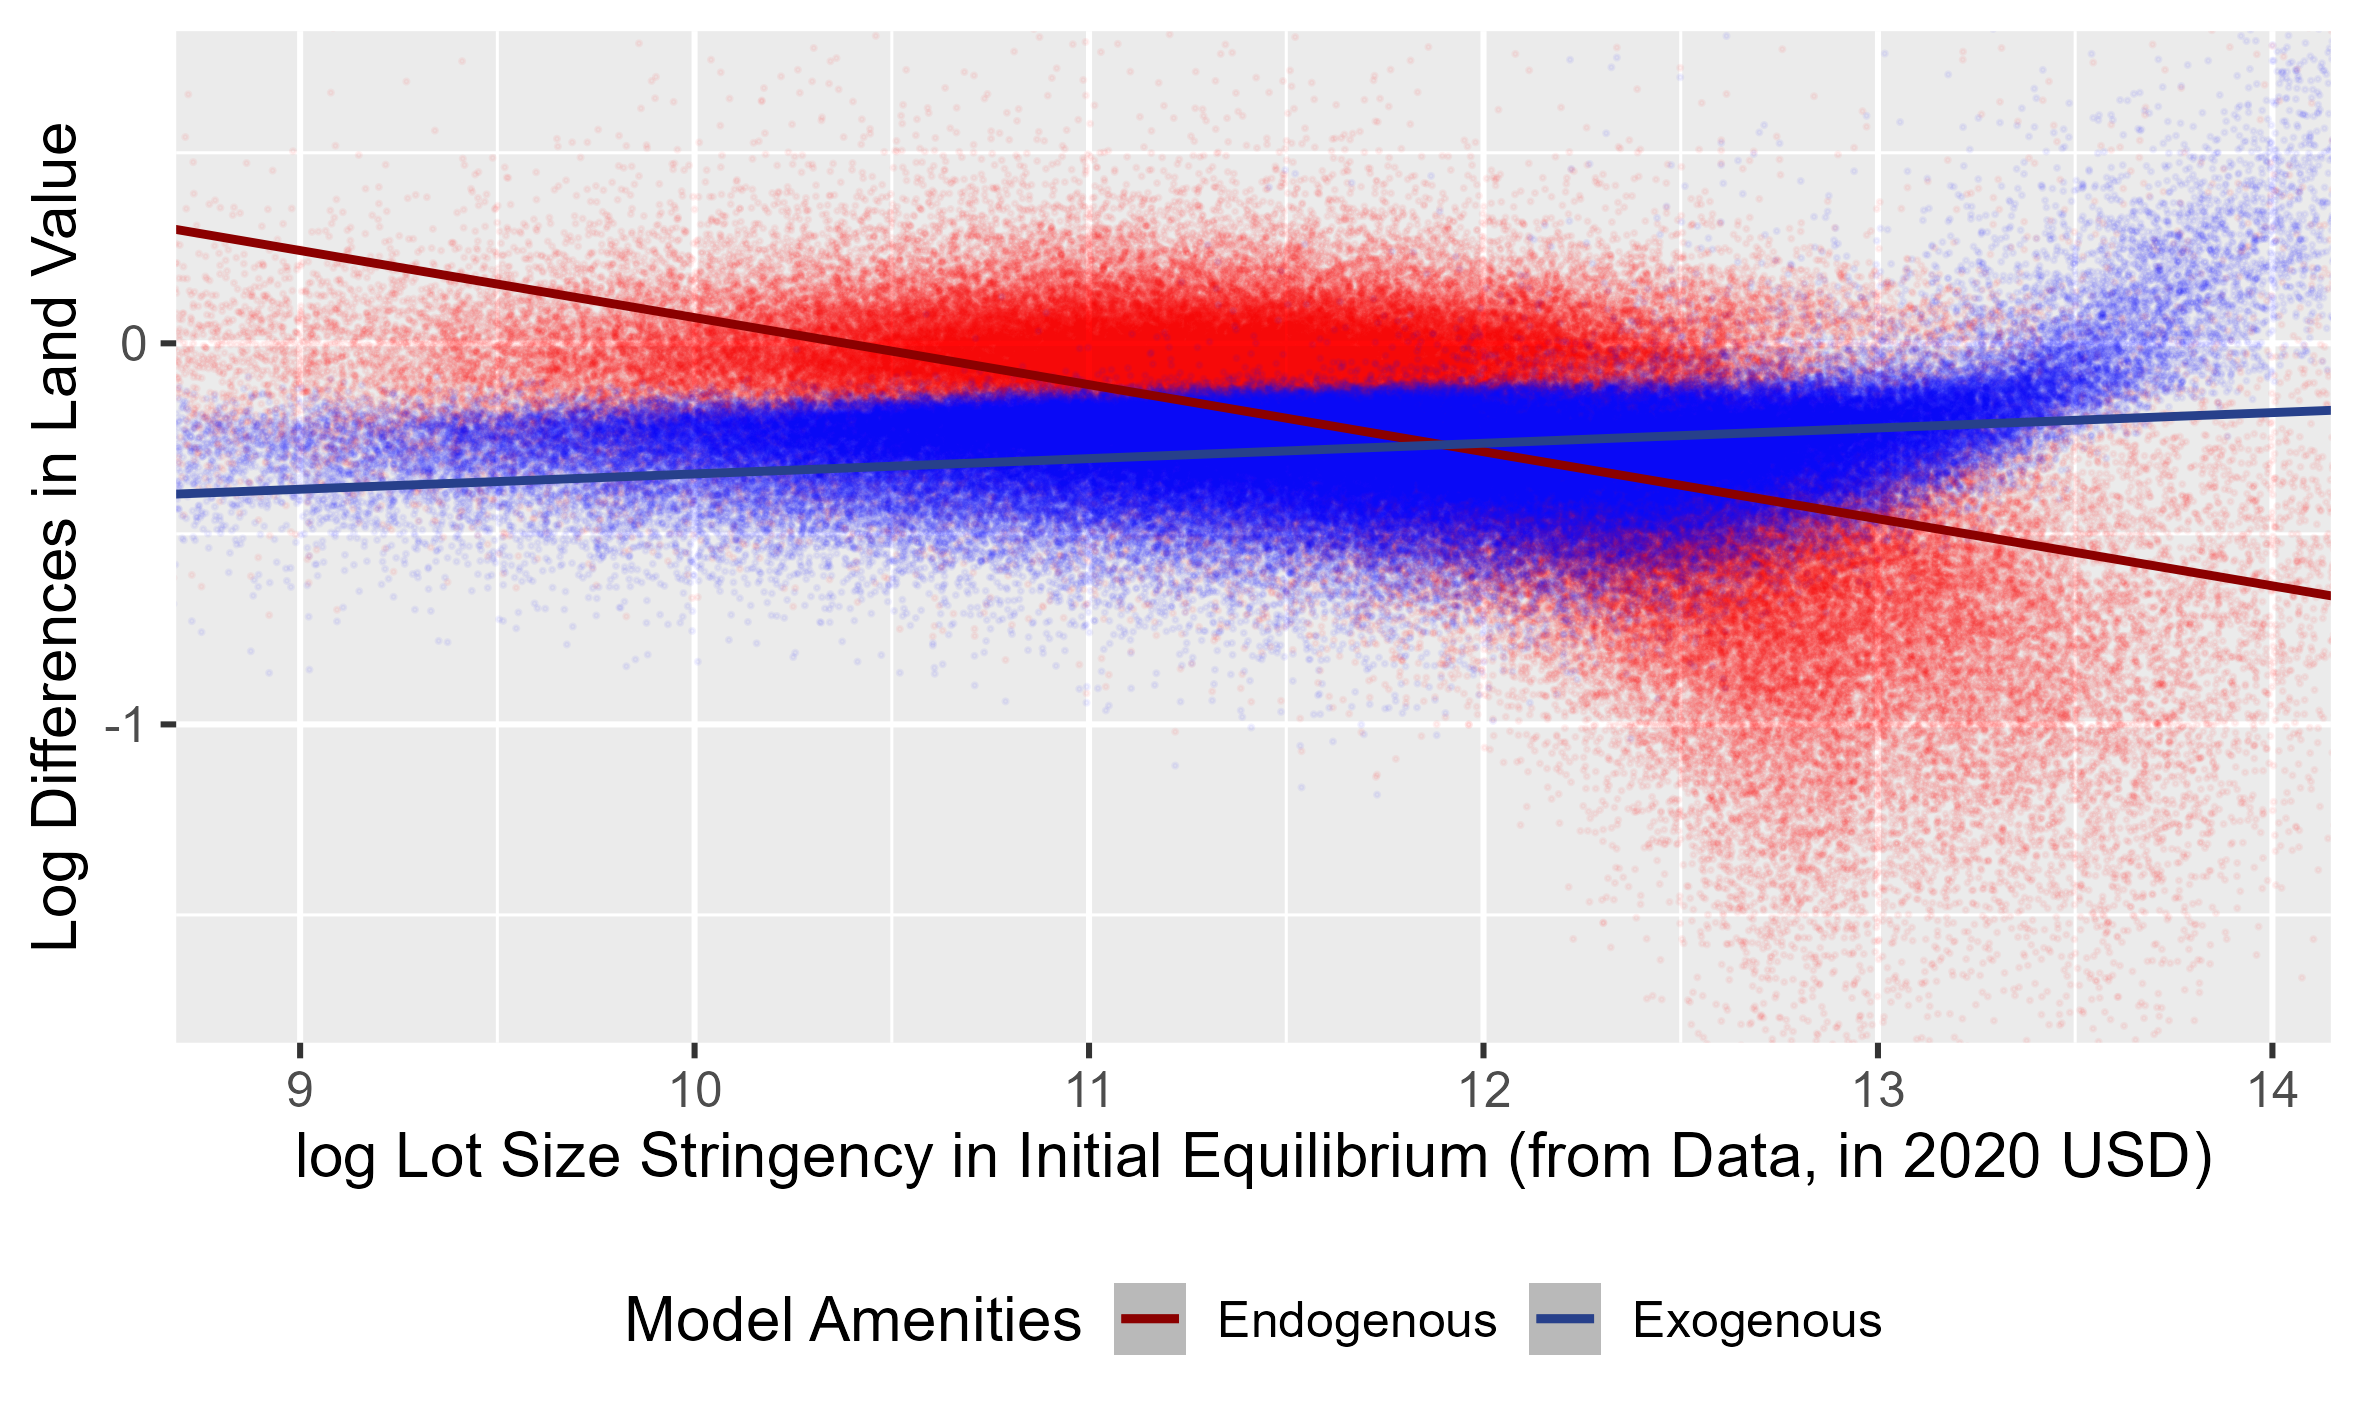
\includegraphics[width=\textwidth]{StringencyChangeLandVal.png}}
		
		\caption*{Changes in land values by regulatory stringency in the baseline equilibrium (from Equation \ref{observedStringency}). Data generated from the endogenous amenities counterfactual is scattered in black. Linear fits on data generated by endogenous and exogenous amenity counterfactuals are in red and blue, respectively.}
		
	\end{figure}
	
	\clearpage
	
	\begin{figure}\caption{ \\ San Francisco, initial data and counterfactual outcomes.}\label{figure:SF_ctfl}
	\makebox[\textwidth]{\includegraphics[width=1.2\textwidth, height = 0.7\textheight]{SF_combined.png}}
	
	\caption*{San Francisco's initial data on income and regulatory stringency, along with changes in incomes and land values after halving the minimum lot size. Values are binned by quartile for improved readability of the graph. Regulatory stringency is the empirical measure introduced in Equation \eqref{observedStringency}.}
		
	\end{figure}
	
	
	
	\begin{figure}[htbp!]
		\begin{center}
			\caption{ \\ Effects of permuted regulation scheme \\ pooled over renters and homeowners and including capital losses }\label{figure:pooledWelfare_optPolicy}
				\makebox[\textwidth]{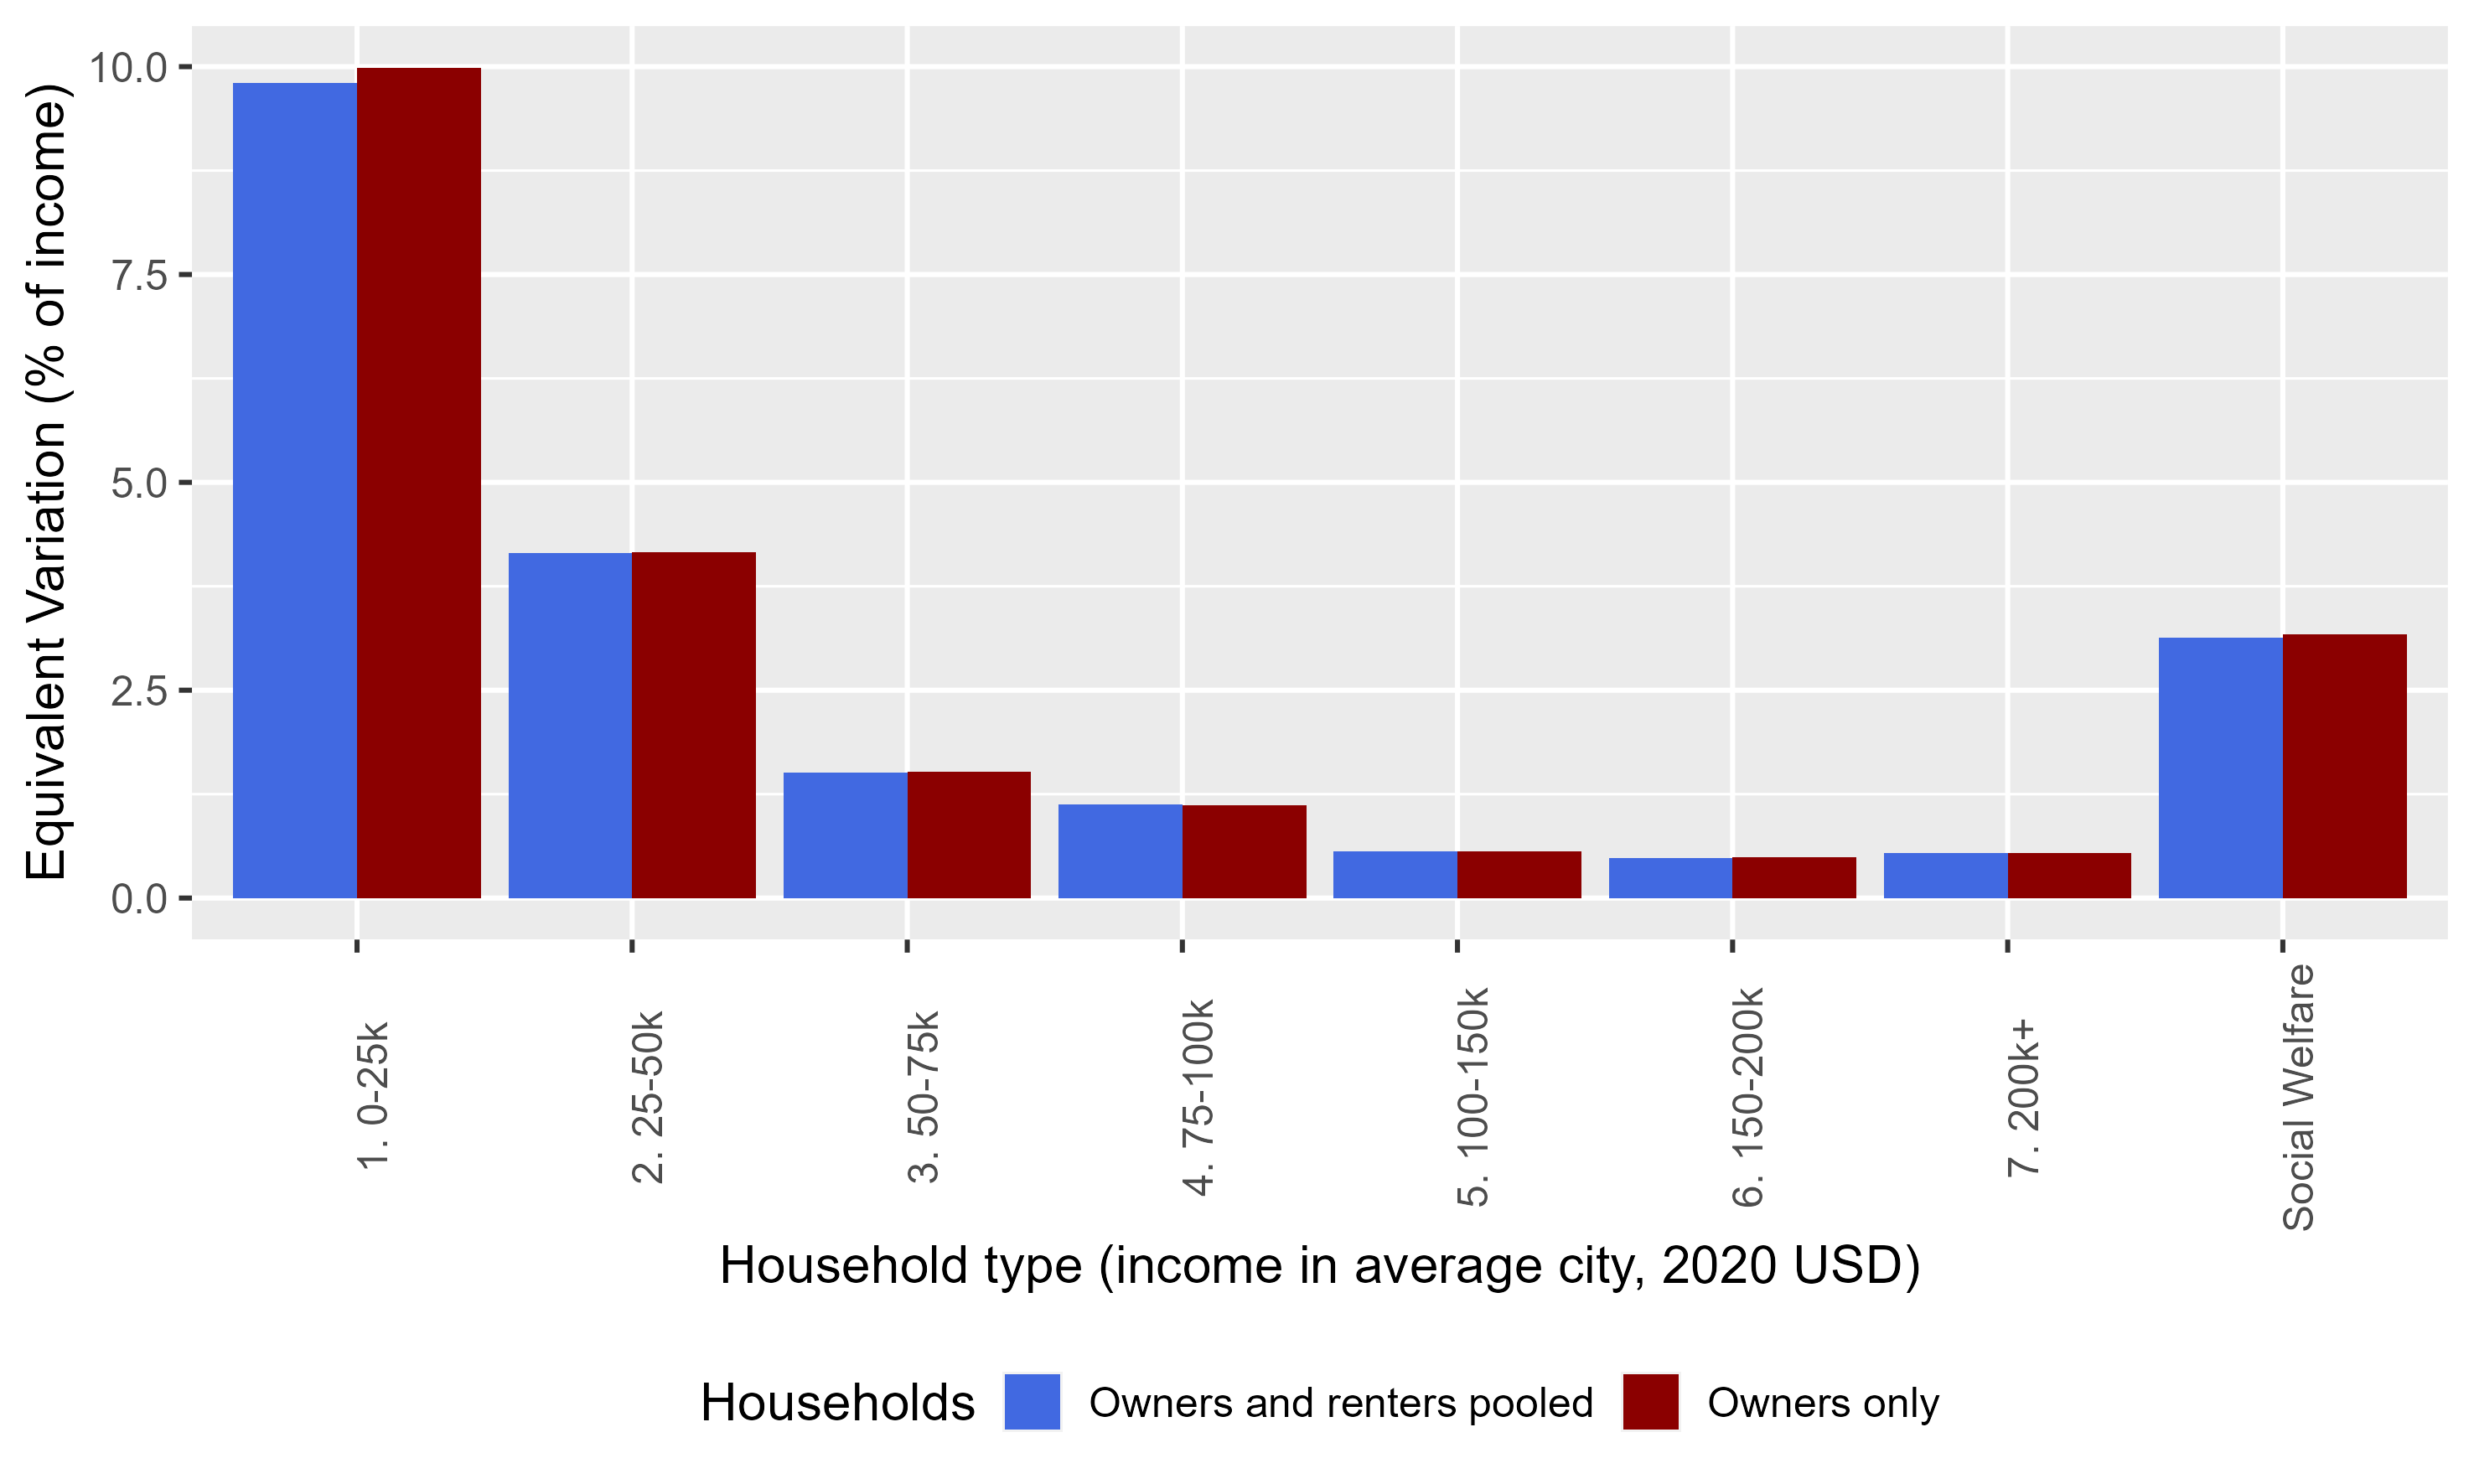
\includegraphics[width=1.1\textwidth]{WelfarePooled_optPolicy.png}}
		\end{center}
			\caption*{Welfare is measured as the equivalent variation and expressed as a percentage of initial income. Higher values mean higher welfare gains. Social welfare is the population weighted average of welfare by type. Results incorporate capital losses for homeowners by income type, using a procedure outlined in Appendix \ref{Appendix:RenterLandownerWelfare}. Results include equilibrium adjustments to neighborhood amenity value as in the baseline counterfactual. Renters and homeowners are pooled by type using a population-weighted average of welfare changes.}
		\end{figure}
		

	
	
	\clearpage
	
	\section*{Tables}
	\begin{center}
		\centering
	
		\begin{table}[htbp]
			\caption{Baseline IV Estimates by income group.}\label{table:baselineIV}
			\makebox[\textwidth]{	
\begin{tabular}{lccc} \hline
 & (1) & (2) & (3) \\
VARIABLES & ln Amenity (Low) & ln Amenity (Med) & ln Amenity (High) \\ \hline
\vspace{4pt} & \begin{footnotesize}\end{footnotesize} & \begin{footnotesize}\end{footnotesize} & \begin{footnotesize}\end{footnotesize} \\
ln Income & 0.1303*** & 0.2805*** & 0.2960*** \\
\vspace{4pt} & \begin{footnotesize}(0.0326)\end{footnotesize} & \begin{footnotesize}(0.0443)\end{footnotesize} & \begin{footnotesize}(0.0330)\end{footnotesize} \\
Slope Control & -0.0020** & -0.0029*** & -0.0015* \\
\vspace{4pt} & \begin{footnotesize}(0.0008)\end{footnotesize} & \begin{footnotesize}(0.0011)\end{footnotesize} & \begin{footnotesize}(0.0008)\end{footnotesize} \\
Local Slope Control & -0.0002 & -0.0009 & -0.0017*** \\
\vspace{4pt} & \begin{footnotesize}(0.0007)\end{footnotesize} & \begin{footnotesize}(0.0008)\end{footnotesize} & \begin{footnotesize}(0.0006)\end{footnotesize} \\
Outer Slope Control & 0.0062* & 0.0052 & 0.0038 \\
 & \begin{footnotesize}(0.0036)\end{footnotesize} & \begin{footnotesize}(0.0042)\end{footnotesize} & \begin{footnotesize}(0.0026)\end{footnotesize} \\
\vspace{4pt} & \begin{footnotesize}\end{footnotesize} & \begin{footnotesize}\end{footnotesize} & \begin{footnotesize}\end{footnotesize} \\
Observations & 170,951 & 171,045 & 165,317 \\
Specification & IV & IV & IV \\
Donut & 0.75-1.25km & 0.75-1.25km & 0.75-1.25km \\
Base Controls & Yes & Yes & Yes \\
Amen/Topo Controls & No & No & No \\
Density Control & No & No & No \\
 FStat Bart c 35 km & 63.4 & 63.4 & 58.5 \\ \hline
\multicolumn{4}{c}{\begin{footnotesize} Standard errors in parentheses\end{footnotesize}} \\
\multicolumn{4}{c}{\begin{footnotesize} *** p$<$0.01, ** p$<$0.05, * p$<$0.1\end{footnotesize}} \\
\end{tabular}

 }
			\caption*{ Columns are ordered by income group. All specifications include MSA fixed effects and standard errors are clustered using a 35km Bartlett kernel. "Donut Slope Control" is the average slope within the block group plus a buffer with length equal to $d_{1}$. "Local Slope Control" is the average slope within the block group. "Outer slope control" is the average slope from $d_{2}$ to 10km. $\ln \text{Income}$ is instrumented with the average slopes of block groups that have centroids within buffer $d_{1}$ and $d_{2}$. "Base Controls" include travel time, building age, public transport and bus shares in commuting and CBD distance. "Amen/Topo" controls include various amenities (density of coffee shops, parks, restaurants) and various topographic features (cover of different types of forest such as deciduous or evergreen, wetlands, perennial snow cover). "Density Control" is the within-MSA density ranking of the block group.}
		\end{table} 
		
	\end{center}
	
	
	\begin{landscape}
		\begin{center}
			\begin{table}[h]
			\caption{Table of calibrated parameters.}\label{table:CalibrationTable}
			\makebox[\linewidth]{\renewcommand{\arraystretch}{1.6}
	\begin{tabular}{|ll|l|l|}
		\hline 
		\textbf{Parameter} & \textbf{Description} & \textbf{Value} & \textbf{Source or Target} \\ 
		\textbf{Housing Demand} &  &  &  \\ 
		$P_{R}(i)$ & Housing prices (regulated zone) & & Hedonic regression using CoreLogic transactions (Section \ref{Calibration:HousingPrices}) \\ 
		$P_{U}(i)$ & Housing prices (unregulated zone) & & ACS fraction of households living in regulated structures (Section \ref{Calibration:HousingPrices2}) \\
		($\beta$, $\bar{A}$) & Housing preference parameters & (0.08, 6000) & ACS aggregate spending on housing services by income (Section \ref{Calibration:HousingPrices2}) \\ \hline 
		\textbf{Neighborhood Demand} &  &  &  \\ 
		$\theta$ & Across-city migration elasticity & 4 & \cite{morettihornbeck}, after rescaling $V(i,z)$ \\ 
		$\rho$ & Within-city migration elasticity & 8.5 & \cite{BSH}, after rescaling $V(i,z)$\\ 
		$b(i, z)$ & Amenity values by skill & & ACS block-group income distribution (Section \ref{Calibration:Amenities}) \\ 
		$w(c)$ & City productivity & & Mincer regression with city fixed effects on ACS household data (Section \ref{Calibration:CityProd}) \\ \hline
		\textbf{Housing Supply} &  &  &  \\ 
		$R(i)$ & Value of a minimal lot & & Data (Fact \ref{FStringency}) \\ 
		$\lambda(i)$ & Construction productivity & & Clear housing markets in each zone (Section \ref{Calibration:HousingSupply})  \\ 
		$T_{o}(i)$ & Land available for construction by zone & & Clear housing markets in each zone (Section \ref{Calibration:HousingSupply})  \\ 
		$\epsilon(i)$ & Housing supply elasticity & & \cite{BSH}  \\ 
		\hline 
	\end{tabular}
}
			\end{table}	
		\end{center}
	\end{landscape}
	
	
	\begin{center}
		\centering
		
		\begin{table}[htbp]
				\caption{Productivity changes from counterfactual by model assumptions.}\label{table:LabourProdDifCtfls}
				\makebox[\textwidth]{	\renewcommand{\arraystretch}{1.25}
\begin{tabular}{lllll}
\hline
\hline
End. Amenities & End. Productivity & Education & Prod. Growth & No income sorting \\ 
\hline
\checkmark  &  &  & 0.26\% & 1.41\% \\ 
&  &  & 0.44\% & 2.14\% \\ 
\checkmark  & \checkmark  &  & 0.5\% & 1.82\% \\ 
\checkmark  &  & \checkmark  & 0.25\% & 1.3\% \\ 
\checkmark  &\checkmark & \checkmark  & 0.46\% & 1.61\%\\ 
\hline
\hline
\end{tabular}


 }
				\caption*{Productivity changes from counterfactual by model assumptions. "Prod. Growth" refers to productivity changes from counterfactual. "No income sorting" refers to calculating what productivity growth would be if cities grew at levels determined by counterfactual, but with no compositional changes to city income or education. For the full model (last row), I ignore how city wages change when calculating the no-income-sorting counterfactual. This is because uniform city growth when productivity is endogenous by education causes income sorting, which, in turn, is due to agglomeration being education-augmenting, as in \cite{ineqincreased}.}
			
		\end{table}
		
		
	\end{center}
	
	\begin{center}
		\begin{table}[htbp]\caption{Local welfare effects of halving the minimum lot size in San Francisco.}\label{table:SF_dereg}
			\makebox[\textwidth]{	\centering \renewcommand*{\arraystretch}{1.6}
\begin{tabular}{lll}
\hline
\hline
Endogenous Amenities & Yes & No \\ 
\hline
\textbf{Renter equivalent variation ($\%$ of income)} & & \\
0-25k & 0.13 & 0.23 \\ 
25-50k & 0.16 & 0.25 \\ 
50-75k & 0.14 & 0.27 \\ 
75-100k & 0.11 & 0.19 \\ 
100-150k & 0.08 & 0.13 \\ 
150-200k & 0.04 & 0.08 \\ 
200k+ & -0.02 &  0.02 \\ 
\textbf{Change in SF Land Values ($\%$)} & -1.60 & 11.81\\ 
\hline
\hline
\end{tabular}


 }
			\caption*{Reported renter welfare is the expected welfare conditional on living in San Francisco. Due to the assumed Gumbel distribution of idiosyncratic shocks, this is also equal to the average welfare of a renter nationally. Welfare is calculated using the equivalent variation and expressed as a percentage of income for each type.}
			
		\end{table}
	\end{center}
	
	
	\clearpage
	
	
	\appendix
	\normalsize
	\section{Appendix: Data and Facts Continued}\label{DataandFactsContinued}
	
	\subsection{Data Construction} \label{Appendix:DataConstruction}
	\paragraph*{}
 In this section, I focus on data used in both the empirical work and estimation of the structural model. This paper uses two broad sources of data: 
	
	\begin{enumerate}
		\item CoreLogic:
		
		\begin{enumerate}
			\item Universe of property assessments (most current assessments as of December 2022) 
			
			\item 2008-2012 and 2015-2022 universe of transactions
		\end{enumerate} 
		
		\item Other data:
		\begin{enumerate}
			\item 2008-2012 and 2016-2020 American Community Survey (ACS) tabulations, harmonized to 2020 block group definitions
			
			\item 2010 and 2020 census housing counts harmonized to 2020 block groups.
			
			\item 2007-2010 and 2016-2017 National Neighborhood Data Archive (NaNDA) data at the tract level. 
			
			\item The US Geological survey's EDNA database (2003 version)
		\end{enumerate}
	\end{enumerate} 
	where the separated data ranges are used to construct two panels over block groups. These two sources are used to construct a block-group level panel:
	
	\begin{enumerate}
		\item \textbf{Minimum lot sizes and land value density}. I defer a discussion of how minimum lot sizes and land value densities are constructed to Appendices \ref{Appendix:ConstructZoningDistricts} and \ref{Appendix:MeasureStringency}, as this requires detail.
		
		\item \textbf{The share of housing units in regulated structures}. These enter into the stringency measure in \eqref{observedStringency}. The ACS reports housing counts for structures between 1, 2, and 3-4 housing units, labeled as \textbf{Units in Structure}. These are aggregated to arrive at household counts in regulated structures. I do not use CoreLogic data to calculate these shares as many assessments in large multifamily structures do not have information on the number of housing units. 
		
		\item \textbf{Block group level densities of housing units and incomes}.  Average incomes and shares of housing units in regulated structures are directly calculated from the ACS tabulations for each panel. Average incomes in each block group are calculated by dividing tabulated aggregate neighborhood income by the number of sampled households\footnote{These tabulations are labeled \textbf{Aggregate Household Income in the Past 12 Months} and \textbf{Housing Units}}. Housing counts used to construct density measures are from the 2020 Census.
		
		\item \textbf{Various controls used in estimation}. These include (from the ACS) median building age, household size; share of cars in commuting, buses and other public transport; shares of households that are families, average travel time, white and college shares; (from NaNDA) density of performing arts facilities, sports, casinos, recreational, transit stops, fast food, restaurants, coffee shops and bars; fraction of land area in parks, covered by perrenial snow, deciduous forest, evergreen, mixed forest, shrubs, herbaceous, woody and herbaceous wetlands. 
		
		\item \textbf{Slopes}. I use the USGS EDNA database at $30 \times 30$m resolution to create average slope measures at the block group level. This data is used solely in the estimation of the effect of income on neighborhood amenity value in Section \ref{Section:EstNeighborhoodChoice}. 
	\end{enumerate}
	
	There are roughly $196,000$ block groups in 2013-definition Metropolitan Statistical Areas (MSAs). To estimate the  regressions in \ref{Figure:IncomeSortingStrong} and \ref{Figure:StringencyStrong}, I remove block groups with less than 25 housing units per square mile, representing about $8000$ block groups ($4 \%$ of the sample). The facts are robust to censoring at a wide range of densities, including not censoring at all. Summary statistics for reported variables above given in Table \ref{table:FactsStats}.
	
	
	\clearpage
	
	\subsection{Constructing Zoning Districts}\label{Appendix:ConstructZoningDistricts} 
	\paragraph*{}
	Block groups generally do not correspond to areas by which local governments assign uniform land use regulation. To measure "bunching" of minimum lot sizes around regulatory levels, I need to take a stand on the geographic unit by which to construct lot size distributions. I call these geographic units "Zoning Districts". More often than not, zoning districts can be inferred from zoning codes reported in the CoreLogic data\footnote{However, no information on specific regulation can be extracted from these codes.}. I assign a zoning code to a block group by taking the modal code across parcels in the block group. Block groups with no populated zoning code data are assigned missing. 
	 
	 \paragraph*{}
	 For roughly $66,000$ block groups (one third of the sample), there is no data on zoning codes to apply regulation. To extend coverage of zoning districts, I cluster the remaining block groups. The fundamental challenge in doing so is a trade-off when choosing the size of these zoning districts: on one hand, large zoning districts may pool together multiple levels of regulation, and there is no way to distinguish between them. On the other hand, zoning districts that are too small may result in spurious measurements due to the lack of observations. I perform the clustering algorithm within each US municipality, as these are typically responsible for setting regulation. I assign at most one municipality to a block group by matching municipalities to geocoded parcels, and taking the modal municipality across parcels. I test the algorithm on two different definitions of a municipality: the municipality reported by CoreLogic for assessment purposes, and the municipality from the US Place Shapefiles.
	
	\paragraph*{} To aggregate block groups into zoning districts, I employ a highly flexible clustering algorithm, which I describe here. This algorithm nests the clustering algorithm of \cite{Chavent2018} and is implemented via their R package. This is useful because it allows for the weighing of two types of variables to assign clusters: geographic proximity and other non-geographic variables. I use block-group modal lot size and first decile of the lot size distribution as these variables. The algorithm allows me to consider how important geographic proximity needs to be relative to other location based characteristics that might signal similar minimum lot sizes. 
	
	\paragraph*{}
	The number of clusters to assign is a parameter in \cite{Chavent2018}'s algorithm. This governs how large zoning districts are. I provide a maximum level of a \textit{targeted average number of block groups per cluster} to as a hyperparameter in the algorithm. This parameter defines the minimum number of clusters that must appear in a municipality. For example, in a municipality with 100 block groups without zoning codes, and if I impose that the maximum cluster size is roughly 25 block groups, then the minimum number of clusters is roughly 4. Subject to this minimum number of clusters, I select the actual number of clusters to minimize the \textit{silhouette score} on non-geographic variables, which is a metric that assesses both within-cluster similarity and across-cluster dissimilarity and is typically used to assess clustering performance. I consider a range of targeted maximum cluster sizes of 5, 15, 25, 100 and 250 block groups, respectively. 
	
	\paragraph*{}
	Summarizing, my algorithm incorporates three important hyperparameters:
	
	\begin{enumerate}
		
		\item Two definitions of a municipality. The first is the municipality reported in the assessments. The second is the incoporated city taken from the US Place shapefiles. If block groups are not in a reported municipality, I treat the county as a municipality instead\footnote{Unincorporated locations typically have land use regulation set by the county they are in.}. 
		
		\item The weight of geographic proximity relative to non-geographic variables when assigning clusters \citep{Chavent2018}.
		
		\item Targeted maximum sizes (in number of block groups) for the average cluster.
	
	\end{enumerate}
	
	\paragraph*{}
	The algorithm can be roughly described as follows: 
	
	\begin{algorithm}
	\caption{Clustering}
			
			\begin{itemize}
				\item[] For all hyperparameters do:
				
				\begin{itemize}
					\item[] For all municipalities do:
					
					\begin{enumerate}
						\item Assign block groups with same non-missing zoning code to district
						
						
						\item Cluster remaining block groups choosing number of clusters between 2 and $N - 1$, where $N - 1$ is the number of block groups to be clustered
						
						\item Select desired number of clusters to minimize sillhouette score subject to the minimum number of clusters constraint. All block groups in a cluster are assigned a different zoning code from other clusters.
					\end{enumerate}
					
				\end{itemize}
			\end{itemize}
	
			
		
 	\end{algorithm}
 	
 	
 	
 	Figure \ref{figure:ZoningDistricts} shows the optimal set of zoning districts for Hayward in the San Francisco metropolitan area (optimal will be defined shortly). The optimal algorithm places largest weight on geographic proximity when assigning clusters. The algorithm also uses a maximum cluster size of 5 block groups, as well as CoreLogic's municipality definition. The average zoning district (including block groups that have missing and non-missing zoning codes) has 3.3 block groups, with a standard deviation of 11. The median size of a zoning district is one block group. Clusters are not sensitive to choices of other hyperparameters; I provide more discussion when assessing the performance of the algorithm in Appendix \ref{Appendix:ValidateStringency}.  
 	
	\begin{figure}[htbp!]
	\caption{Zoning Districts in Hayward, California}\label{figure:ZoningDistricts}
	\makebox[\textwidth]{\includegraphics[width=\textwidth]{HaywardZoningDistricts.png}}
	
	\end{figure}
 	
 	
 	\clearpage
	\subsection{Measuring Minimum Lot Sizes and Stringency}\label{Appendix:MeasureStringency}
	
	\paragraph*{}
	The zoning districts give a set of geographic boundaries for which to measure "bunching" in the lot size distribution. I use the mode of the distribution as a measure of this bunching. Within each zoning district, I take the modal lot size for single family homes, duplexes, triplexes and fourplexes, and adjust the lot size by the implied number of housing units per lot (for example, dividing the minimum lot size by 2 for duplexes). This is useful because municipalities often assign different lot size restrictions to these four different types of structures. I define the \textit{baseline unit density restriction} as the minimum of these to be as conservative as possible, as detecting bunching alone cannot measure regulations pertaining to which of these four structures are allowed to be built. This minimum is the unit density restriction that is used both in the facts and in the calibration of the model. 
	
	\paragraph*{}
	To build intuition behind why the mode is an accurate measure of bunching, consider the distribution of lot sizes in Hayward, California. The official minimum lot size for most of Hayward's zoning districts is 5000 square feet. The mode of the observed distribution of lots in Hayward is also 5000 square feet, as shown below. Mostly all block groups in Hayward are assigned the 5000 square foot minimum lot size with this measurement procedure. 
	
	\begin{figure}[htbp!]
		\caption{Lot size distribution in Hayward, California}\label{figure:Bunching}
		\makebox[\textwidth]{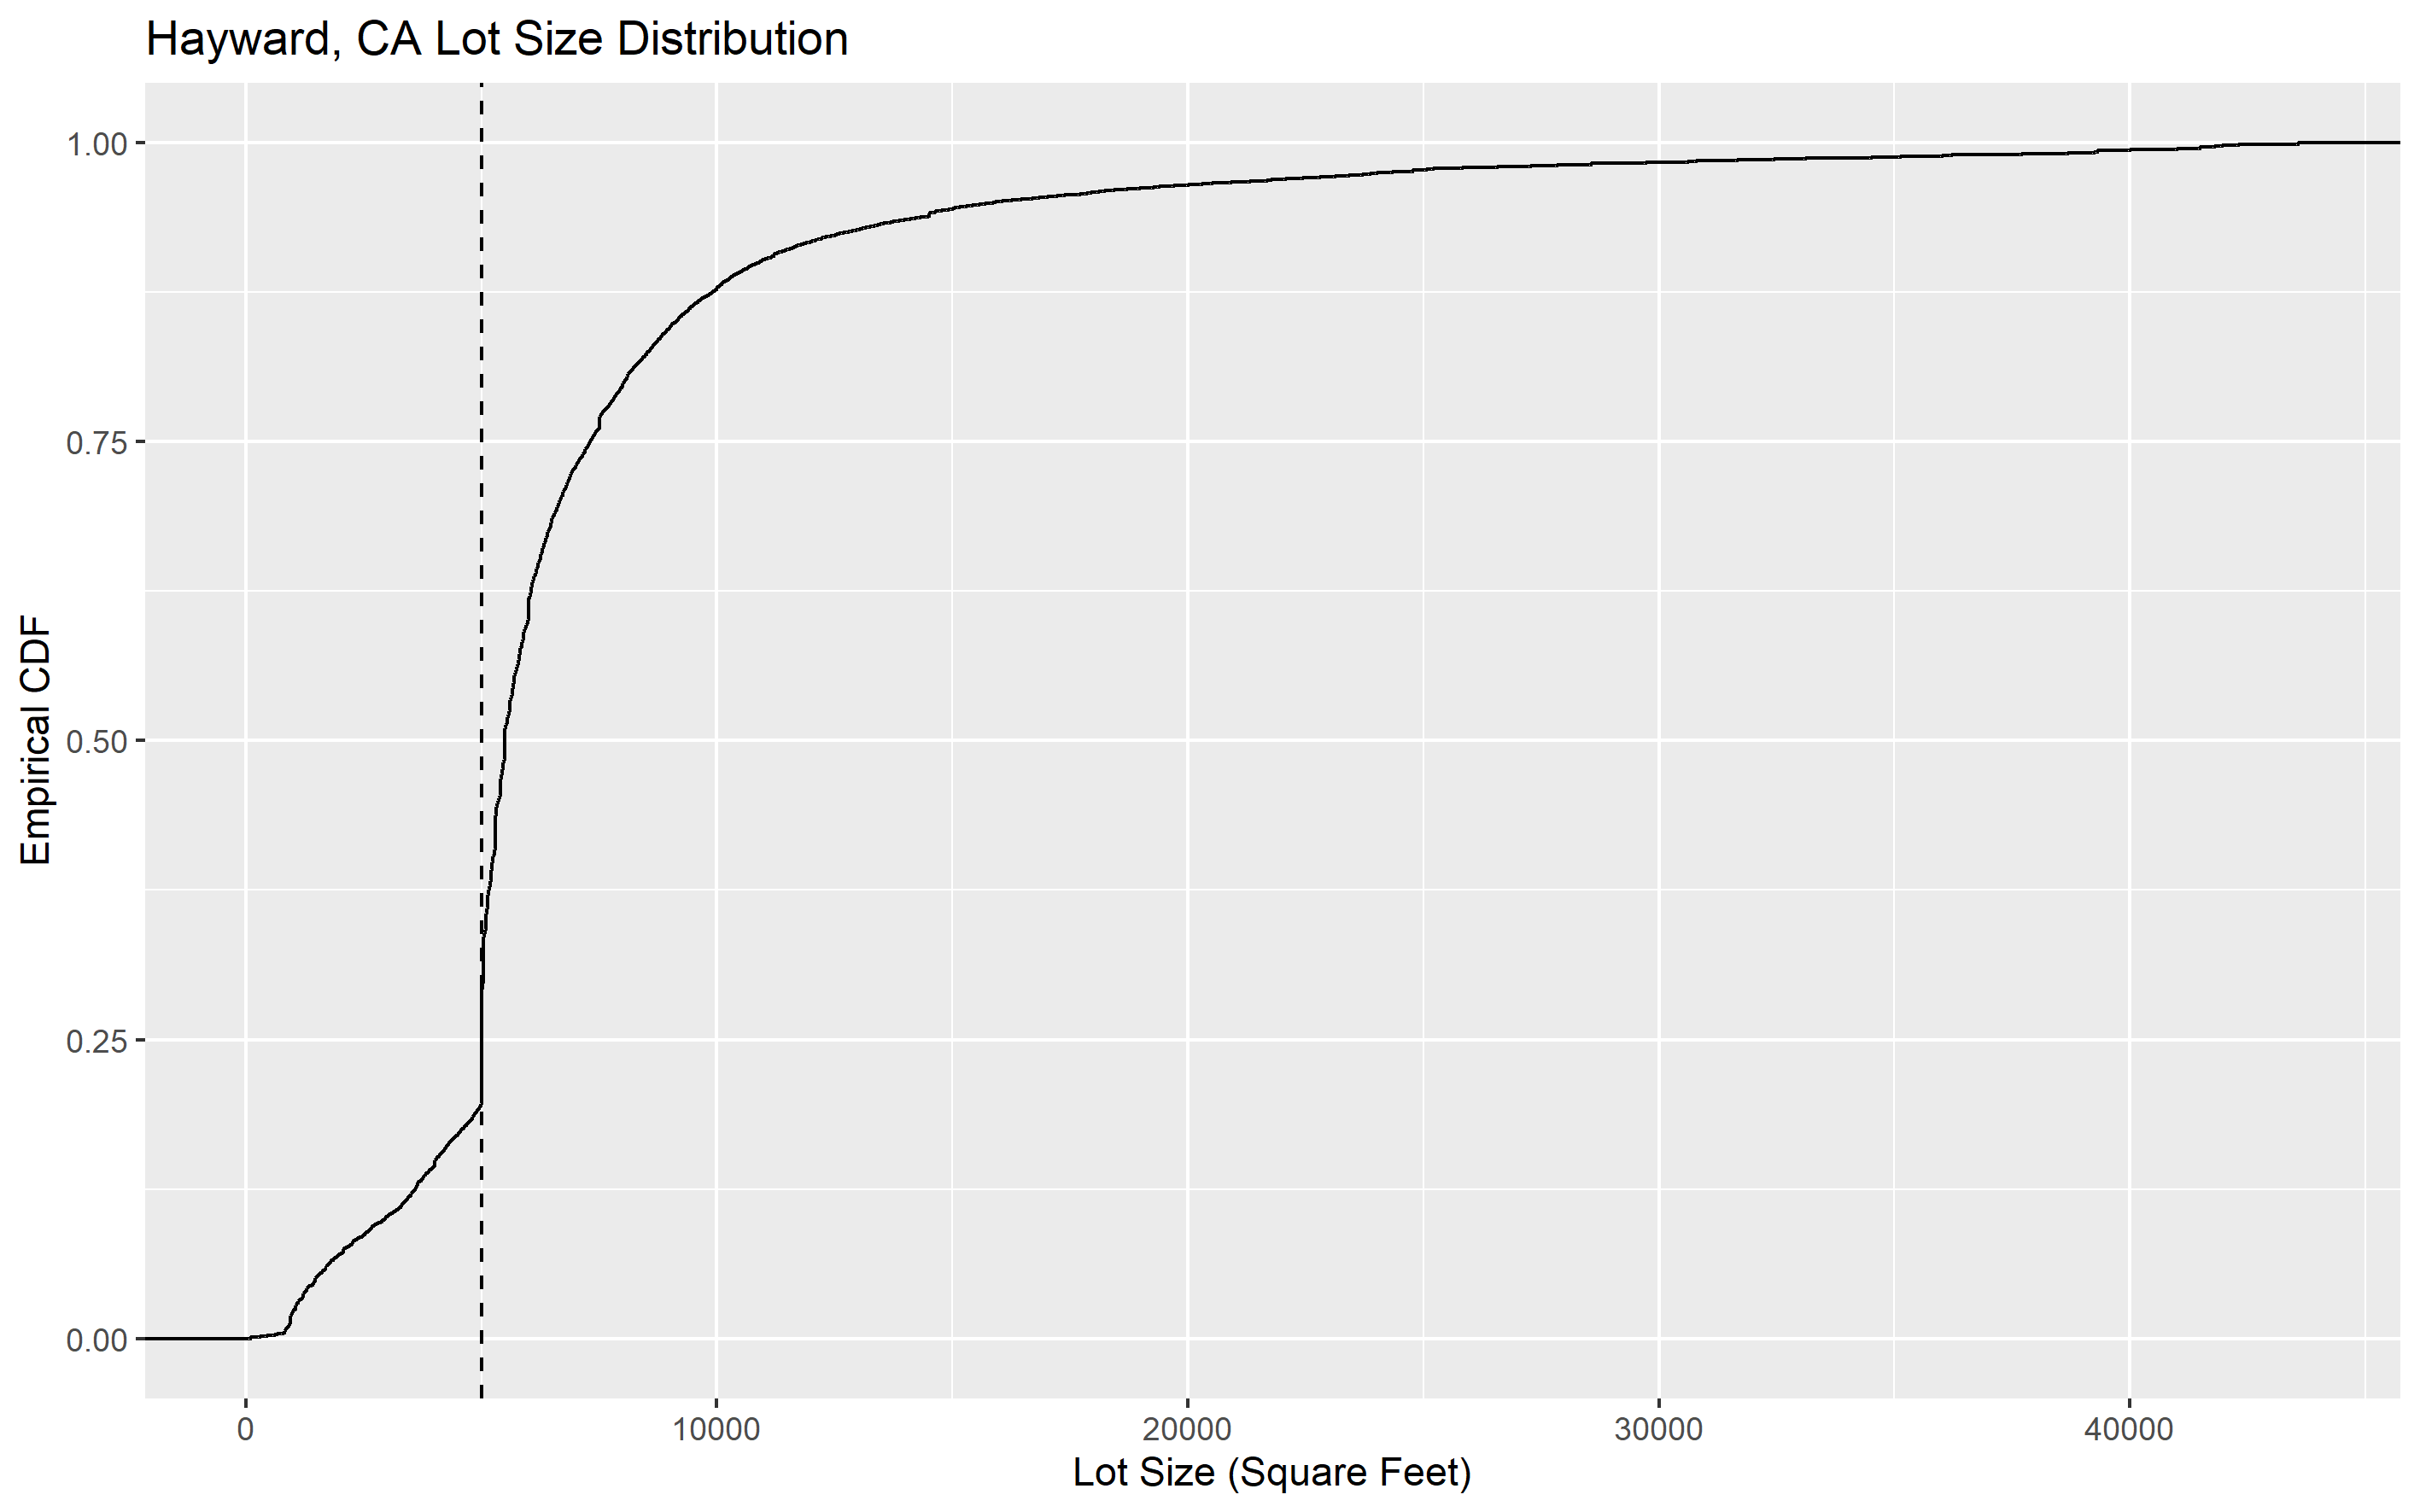
\includegraphics[width=\textwidth]{HaywardLotSizeDist.png}}
		
	\end{figure}
	
	\paragraph*{Land value density}
	Next, I outline how I measure the density of land values, which enters into the measure of regulatory stringency in Equation \eqref{observedStringency}. I limit the sample to \textit{regulated structures} (single family, duplex, triplex and fourplexes) as the only use for land value density pertains to the stringency of regulation (in both the model and the empirical work). I deviate from directly calculating the density of land values (for example, by taking the median sales value across regulated structures and dividing by the median lot size for each block group). This is because land value density varies significantly within block groups between houses with small lots and those with large lots; this leads to large measurement error in regulatory stringency when the measured minimum lot size deviates from the median lot size within a neighborhood.
	
	\paragraph*{}
	Instead, I predict land value densities \textit{at the minimal lot} using a linear model. Within each MSA, I estimate the following regression over assessments indexed by $a$ in neighborhood $i$ and city $c$
	
	\begin{equation}
		\text{LandValue}_{aic} = \beta_{0ic} + \beta_{1c}\text{LotSize}_{aic} + \epsilon_{aic}
	\end{equation}
	The slope parameter of this model informs about the relative price of houses on small lots relative to large lots within the same MSA. I then use the $\beta_{1c}$ parameters from these regressions to predict the land value of the minimal lot in every neighborhood $i$ using the formula 
	\begin{equation}
	 \text{PredLandValue}_{ic} = \text{MedianLandValue}_{ic} - \beta_{1c}\text{MedianLotSize}_{ic} + \beta_{1c}\text{MinLotSize}_{ic}
	\end{equation}
	where $\text{MinLotSize}_{ic}$ is the measured minimum lot size (ignoring implicit unit density restrictions, such as dividing by 2 if duplexes are allowed). This formula ensures that if the minimum lot size is also at the median in the lot size distribution, then its land value is also predicted to be the median land value of the neighborhood\footnote{This often occurs in neighborhoods with extreme "bunching" -- where most lots are built at the minimum.}. Finally, I measure land value densities as 
	
	\begin{equation}
		\text{LandValueDensity}_{ic} = \text{PredLandValue}_{ic}/\text{MinLotSize}_{ic}
	\end{equation}
	which enter directly into the stringency measure, Equation \eqref{observedStringency}.
	
	
	\paragraph*{Additional cleaning} I perform additional cleaning to ensure my measure of regulatory stringency is not wrought with measurement error and other pathologies. I list each procedure below:
	
	\begin{enumerate}
		\item Transactions data are particularly sparse in small and inexpensive cities. This means that there are select block groups in small cities that report massive home values relative to nearby block groups, which makes the measure of regulatory stringency large. This is driven by measurement error when using observed transactions to estimate the transaction value of a median home in these block groups. In cities that report a median transaction below 300k USD (below the US average), I impute block groups median transaction value to the MSA median if it is above 1 million USD. This imputation has the effect of limiting measurement error that compounds in model counterfactuals, making some cities look artificially more stringent then they plausibly are; driven by only a handful of block groups that appear extremely stringent for spurious reasons. Conclusions of counterfactual exercises remain the same whether or not I do this cleaning.
		
		\item Sometimes, the algorithm fails in the sense that the size of the measured minimum lot size is well above the average lot size in some block groups. This usually happens in remote locations where parcels are sparse and their size idiosyncratic. For model counterfactuals and to estimate the facts, I set the observed minimum lot size to zero if the assigned minimum lot size is twice the average. The facts and model counterfactuals are robust to different thresholds for which to perform this cleaning; including no cleaning at all. 
	\end{enumerate}
	
	
	\paragraph*{}
	In Table \ref{table:FactsStats}, I report summary statistics of the measured unit density restrictions, land value densities, and the accompanying measure of regulatory stringency from Fact \ref{FStringency}.  The average unit density restriction across block groups is 0.272 acres per housing unit with a standard deviation of 3.74. Table \ref{table:BoxplotStringency} additionally reports boxplots of stringency for select cities. Figure \ref{figure:MinLotSizeExample} shows the measured unit density restrictions for Hayward, California by zoning district. 
	
	\begin{figure}[htbp!]
		\caption{Hayward Unit density restrictions}\label{figure:MinLotSizeExample}
		\makebox[\textwidth]{\includegraphics[width=\textwidth]{HaywardMinimumLotSizes.png}}
		
	\end{figure}
	
	\clearpage
	\subsection{Validating Minimum Lot Sizes}\label{Appendix:ValidateStringency}
	\paragraph*{}
	To validate the algorithm and to select clustering hyperparameters, I introduce two sources of official data on minimum lot sizes (or more generally, unit density restrictions). The first source, which mirrors validation exercises in \cite{Song} and \cite{Cui}, is the Terner California Land Use Survey (TCLUS). This source of data is aggregated to the municipality level and cannot be used to test how well the algorithm performs on microgeographic variation in regulation. The second data source -- official zoning maps for 13 large US cities -- addresses this limitation. I address how the validation procedure works for each source below. 
	
	\paragraph*{TCLUS} The TCLUS reports minimum lot sizes for both single family homes and "multifamily homes" at the municipality level for over 200 Californian municipalities. As recognized by \cite{Song}, performing validation when the constructed measure of regulation varies within municipalities is difficult. Notwithstanding, I assume the TCLUS data reports the median minimum lot size (weighted by population) for each of these structure types (single family and multifamily). 
	\paragraph*{}
	I take, at the municipality level, the median modal lot across block groups separately for single family homes, duplexes, triplexes and fourplexes (recall that the measured unit density restriction in a neighborhood is the minimum of each of these modes after adjusting for the implied number of units per lot). In each municipality, I match the TCLUS-reported minimum lot size for single family homes with the modal single family lot. I also match the TCLUS-reported minimum lot size for multifamily structures with the closest modal lot amongst duplexes, triplexes, and fourplexes. I then calculate the \textit{error rate} for each municipality level as the smallest error between reported and observed amongst the errors calcuated for both single family and multifamily structures. On this sample of municipalities, the median error on the best set of clustering hyperparameters is $4.5\%$ of the official minimum lot size. For single family homes alone, this error rate is approximately $10\%$. This is very accurate. 
	
	\paragraph*{}
	Note that the unit density restriction actually used in the paper is the minimum across single family homes, duplexes, triplexes and fourplexes, as described in Appendix \ref{Appendix:MeasureStringency}. By definition, this is conservative relative to the minimum lot sizes used to compare to the TCLUS.  
	
	\paragraph*{Official Zoning Maps} I hand collect official zoning maps in 13 large US cities\footnote{These cities are Albany, GA, Atlanta, GA, Berkeley, CA, Cleveland, OH, Columbus, OH, Hayward, CA, Mesa, AZ, Miami, FL, Minneapolis, MN, New Orleans, LA, Oakland, CA and Scottsdale, AZ} and manually match official minimum lot sizes (from their respective online ordinances) to as many zoning codes in these maps as possible. I take into account that some codes allow multifamily structures by calculating the implied unit density restriction in the usual way.
	
	\paragraph*{}
	The difficulty with comparing the measured minimum lot sizes with those reported in the official maps is that my data varies at the zoning district level (a union of block groups), while the official zoning maps vary by official zoning code boundaries. I overlay my zoning districts on the official zoning maps. I then match the closest modal lot amongst single family homes, duplexes, triplexes and fourplexes to data, and calculate an error rate using this closest modal lot. To calcuate the error rate across the entire data, I take the median error across all intersected geography derived from the overlay (the median is weighted such that each block group receives equal weight). This error rate is $16 \%$ of the official unit density restriction at the optimal set of clustering hyperparameters, which is less accurate compared to the TCLUS exercise but still very accurate. For Hayward, California, this error rate is less than $1\%$. This suggests that the efficacy of the algorithm will vary across space, favouring municipalities where the minimum lot size is likely to bind. Reassuringly, performance of the algorithm doesn't vary much across hyperparameters, which implies we are not over-fitting the data used to test. 
	
	
	\clearpage
	
	\subsection{Summary Statistics}\label{Appendix:FactsSummaryStats}
	\begin{table}[htbp!]	
		\caption{Regulatory stringency boxplot for select cities.}\label{table:BoxplotStringency}
		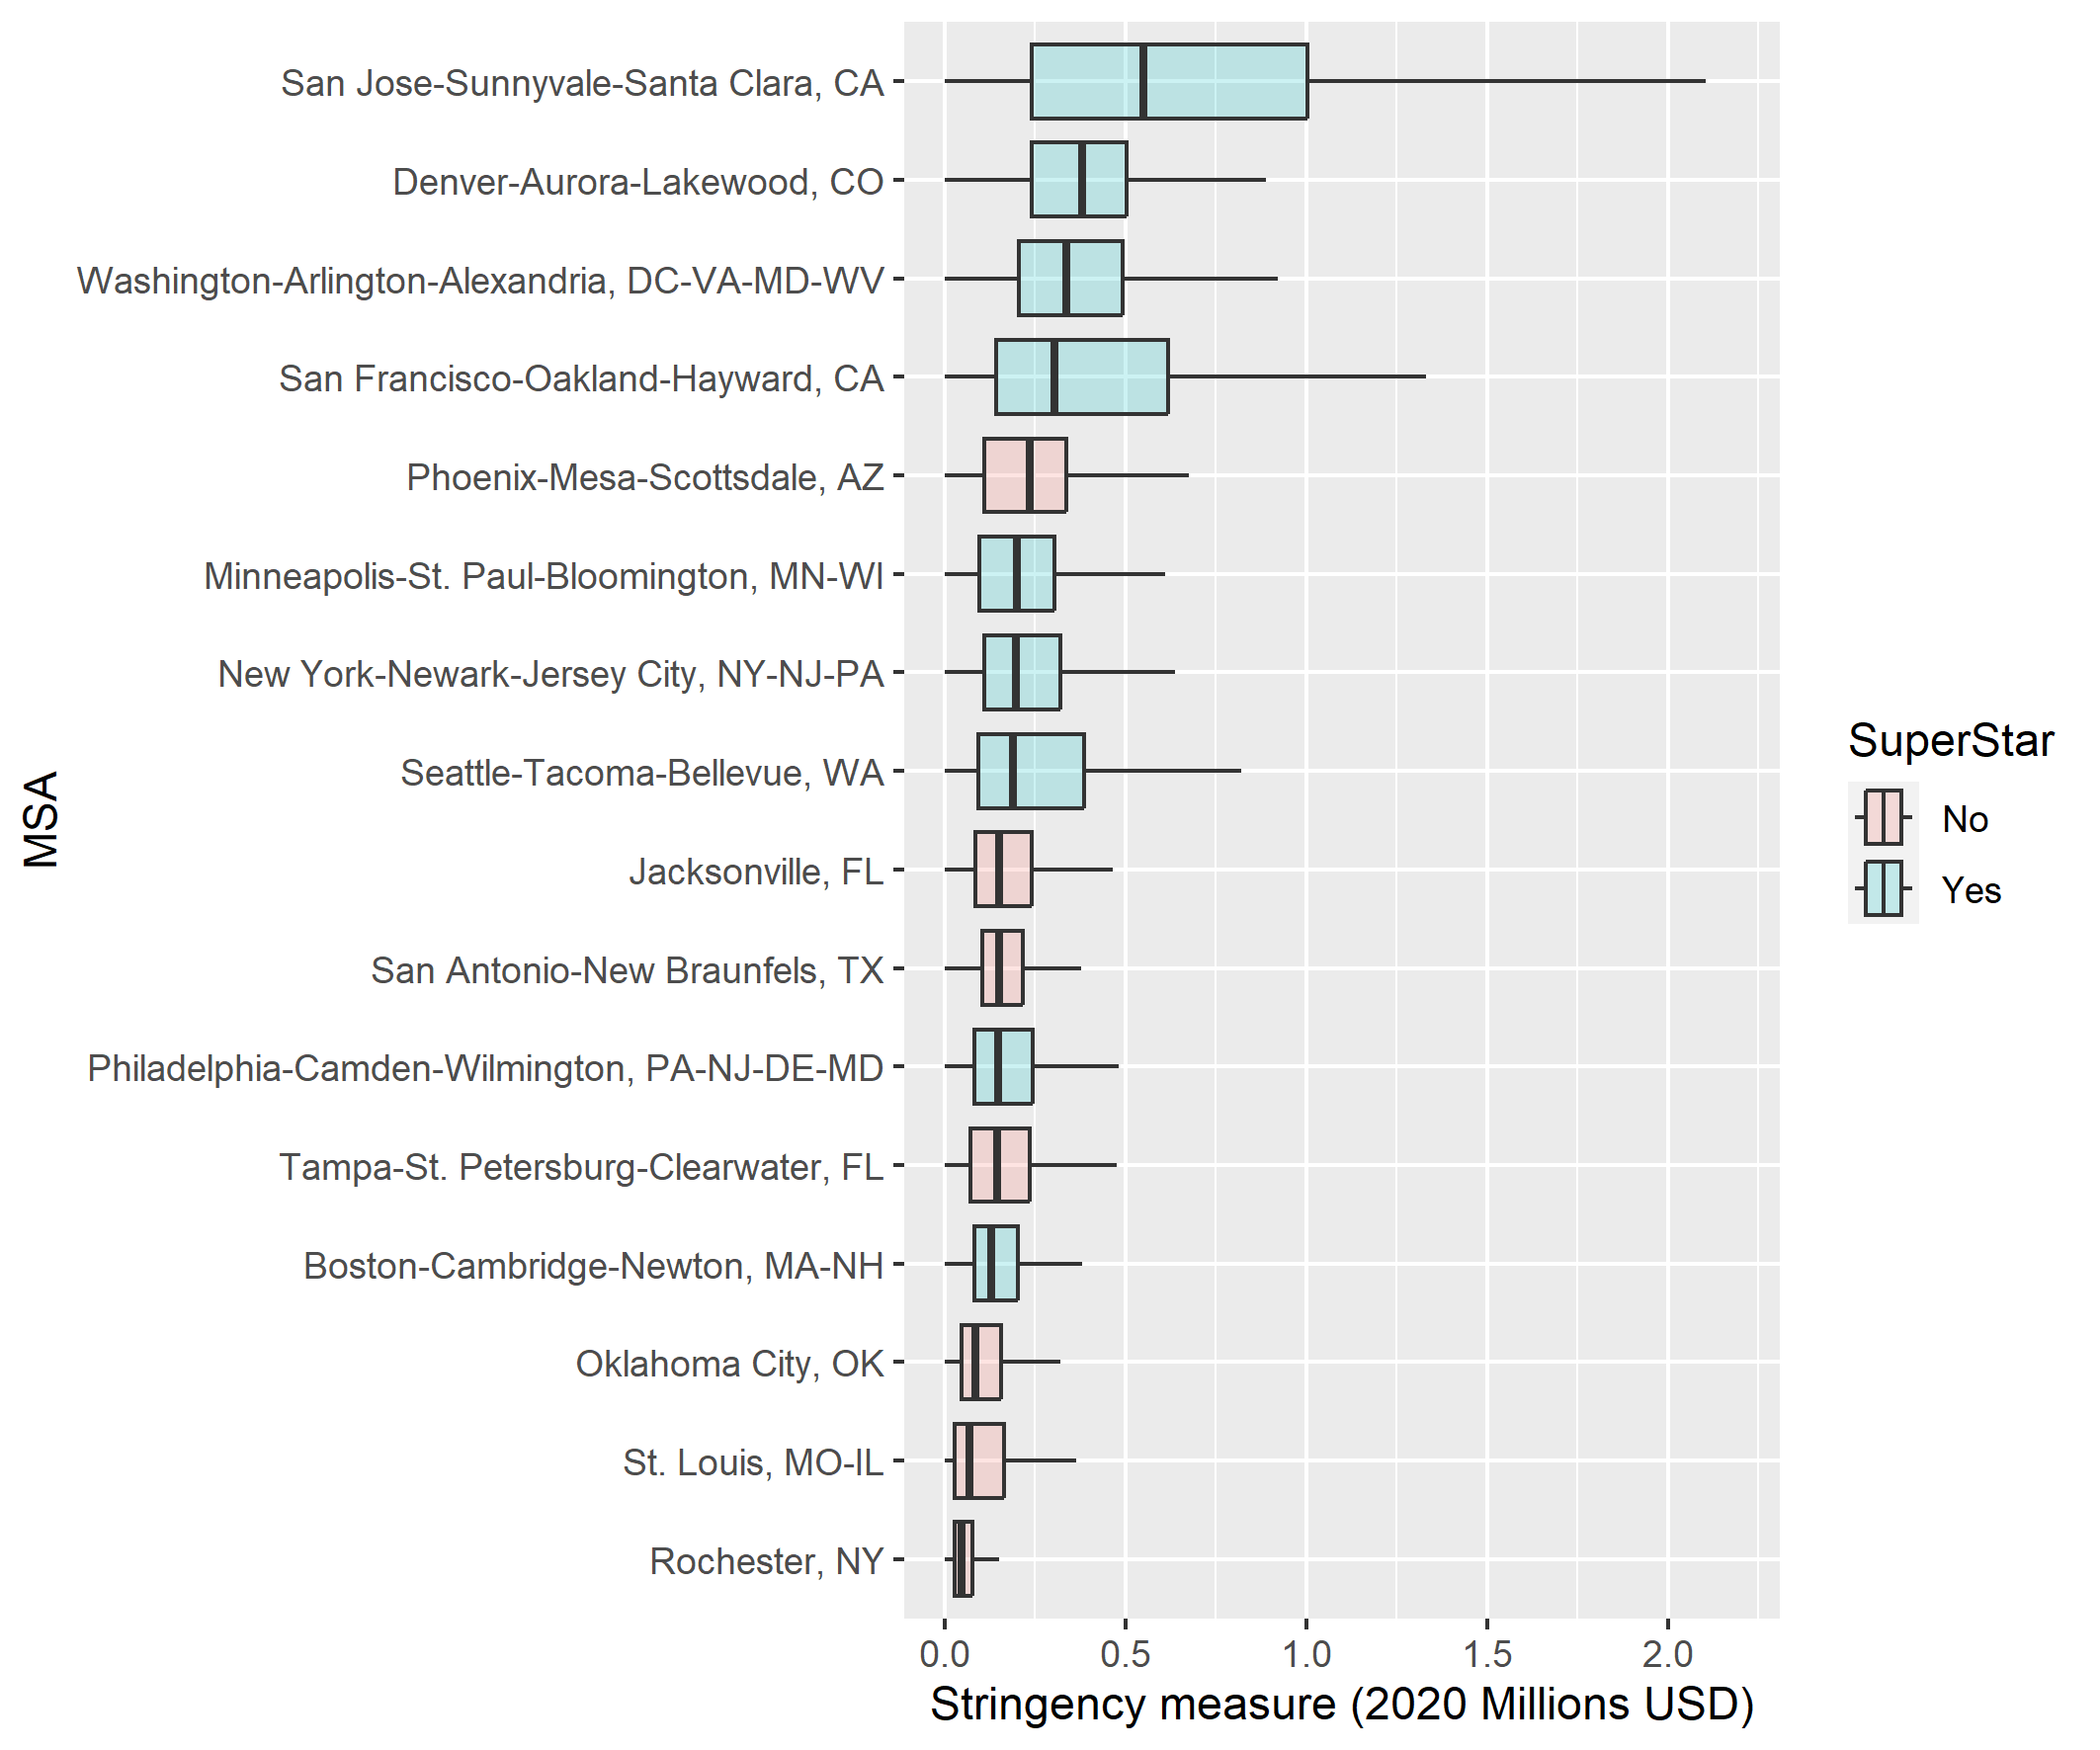
\includegraphics[width=\textwidth]{Facts_incomeStringency_boxplot.png}
		\caption*{Regulatory stringency boxplot for select cities. Reports stringency measure introduced in Equation \eqref{observedStringency} for select cities. Cities are colored based on whether they are included in the superstar sample used to construct Facts \ref{FIncomeDens} and \ref{FStringency}. }
	\end{table}
	
	\clearpage
	
	
	\begin{landscape} 
		\begin{center}
	\begin{table}[h]
		
		\caption{Summary Statistics for Key Variables, \\
					 disaggregated by superstar city status}
		
		\makebox[\linewidth]{\renewcommand{\arraystretch}{1.75}
\resizebox{0.9\textwidth}{!}{
\begin{tabular}{lrrrrrrrrrrrr}
\hline
\hline
SuperStar city & \multicolumn{4}{c}{Aggregate} & \multicolumn{4}{c}{No} & \multicolumn{4}{c}{Yes}  \\ 
 Variable & \multicolumn{1}{c}{N} & \multicolumn{1}{c}{Mean} & \multicolumn{1}{c}{Sd} & \multicolumn{1}{c}{Median} & \multicolumn{1}{c}{N} & \multicolumn{1}{c}{Mean} & \multicolumn{1}{c}{Sd} & \multicolumn{1}{c}{Median} & \multicolumn{1}{c}{N} & \multicolumn{1}{c}{Mean} & \multicolumn{1}{c}{Sd} & \multicolumn{1}{c}{Median} \\ 
\hline 
ln Average Income & 194533 & 11.2 & 0.567 & 11.2 & 83861 & 11 & 0.524 & 11 & 110672 & 11.4 & 0.556 & 11.4 \\ 
Unit Density Restriction (acres) & 182564 & 0.272 & 3.74 & 0.114 & 78743 & 0.338 & 5.18 & 0.138 & 103821 & 0.222 & 2.08 & 0.0861 \\ 
Stringency measure (2020 millions USD) & 179879 & 0.198 & 0.458 & 0.129 & 77316 & 0.124 & 0.111 & 0.0911 & 102563 & 0.254 & 0.592 & 0.172 \\ 
Land Value Density (2020 millions USD/acre) & 187654 & 4.02 & 52.7 & 1.5 & 81657 & 1.53 & 4.82 & 0.859 & 105997 & 5.94 & 70 & 2.46 \\ 
Regulated housing units (share) & 190553 & 0.793 & 0.254 & 0.899 & 82988 & 0.811 & 0.222 & 0.894 & 107565 & 0.778 & 0.275 & 0.904\\ 
\hline
\hline
\end{tabular}
}


}\label{table:FactsStats}
		\caption*{Summary statistics. "Unit Density Restriction" refers to the measured physical unit density restriction that enters into Equation \eqref{observedStringency}, and is measured in Appendix \ref{Appendix:MeasureStringency}. "Regulated Housing Units" refers to the share of housing units in single family homes, duplexes, triplexes and fourplexes. Land Value Density is measured in Appendix \ref{Appendix:MeasureStringency} and enters into \eqref{observedStringency}. "Stringency measure" is the empirical regulatory stringency measure introduced in Equation \eqref{observedStringency}.  Variation in nonmissing data are a result of either 1) incomplete transactions coverage or 2) additional cleaning procedures described in Appendix \ref{Appendix:MeasureStringency}.}
	
	\end{table}		
	\end{center}	
	\end{landscape}
	
	\clearpage

	
	\begin{table}[htbp!]	
		\caption{Relationship between regulatory stringency and productivity.}\label{table:ProductivityStringency}
		\begin{center}
		\makebox[\linewidth]{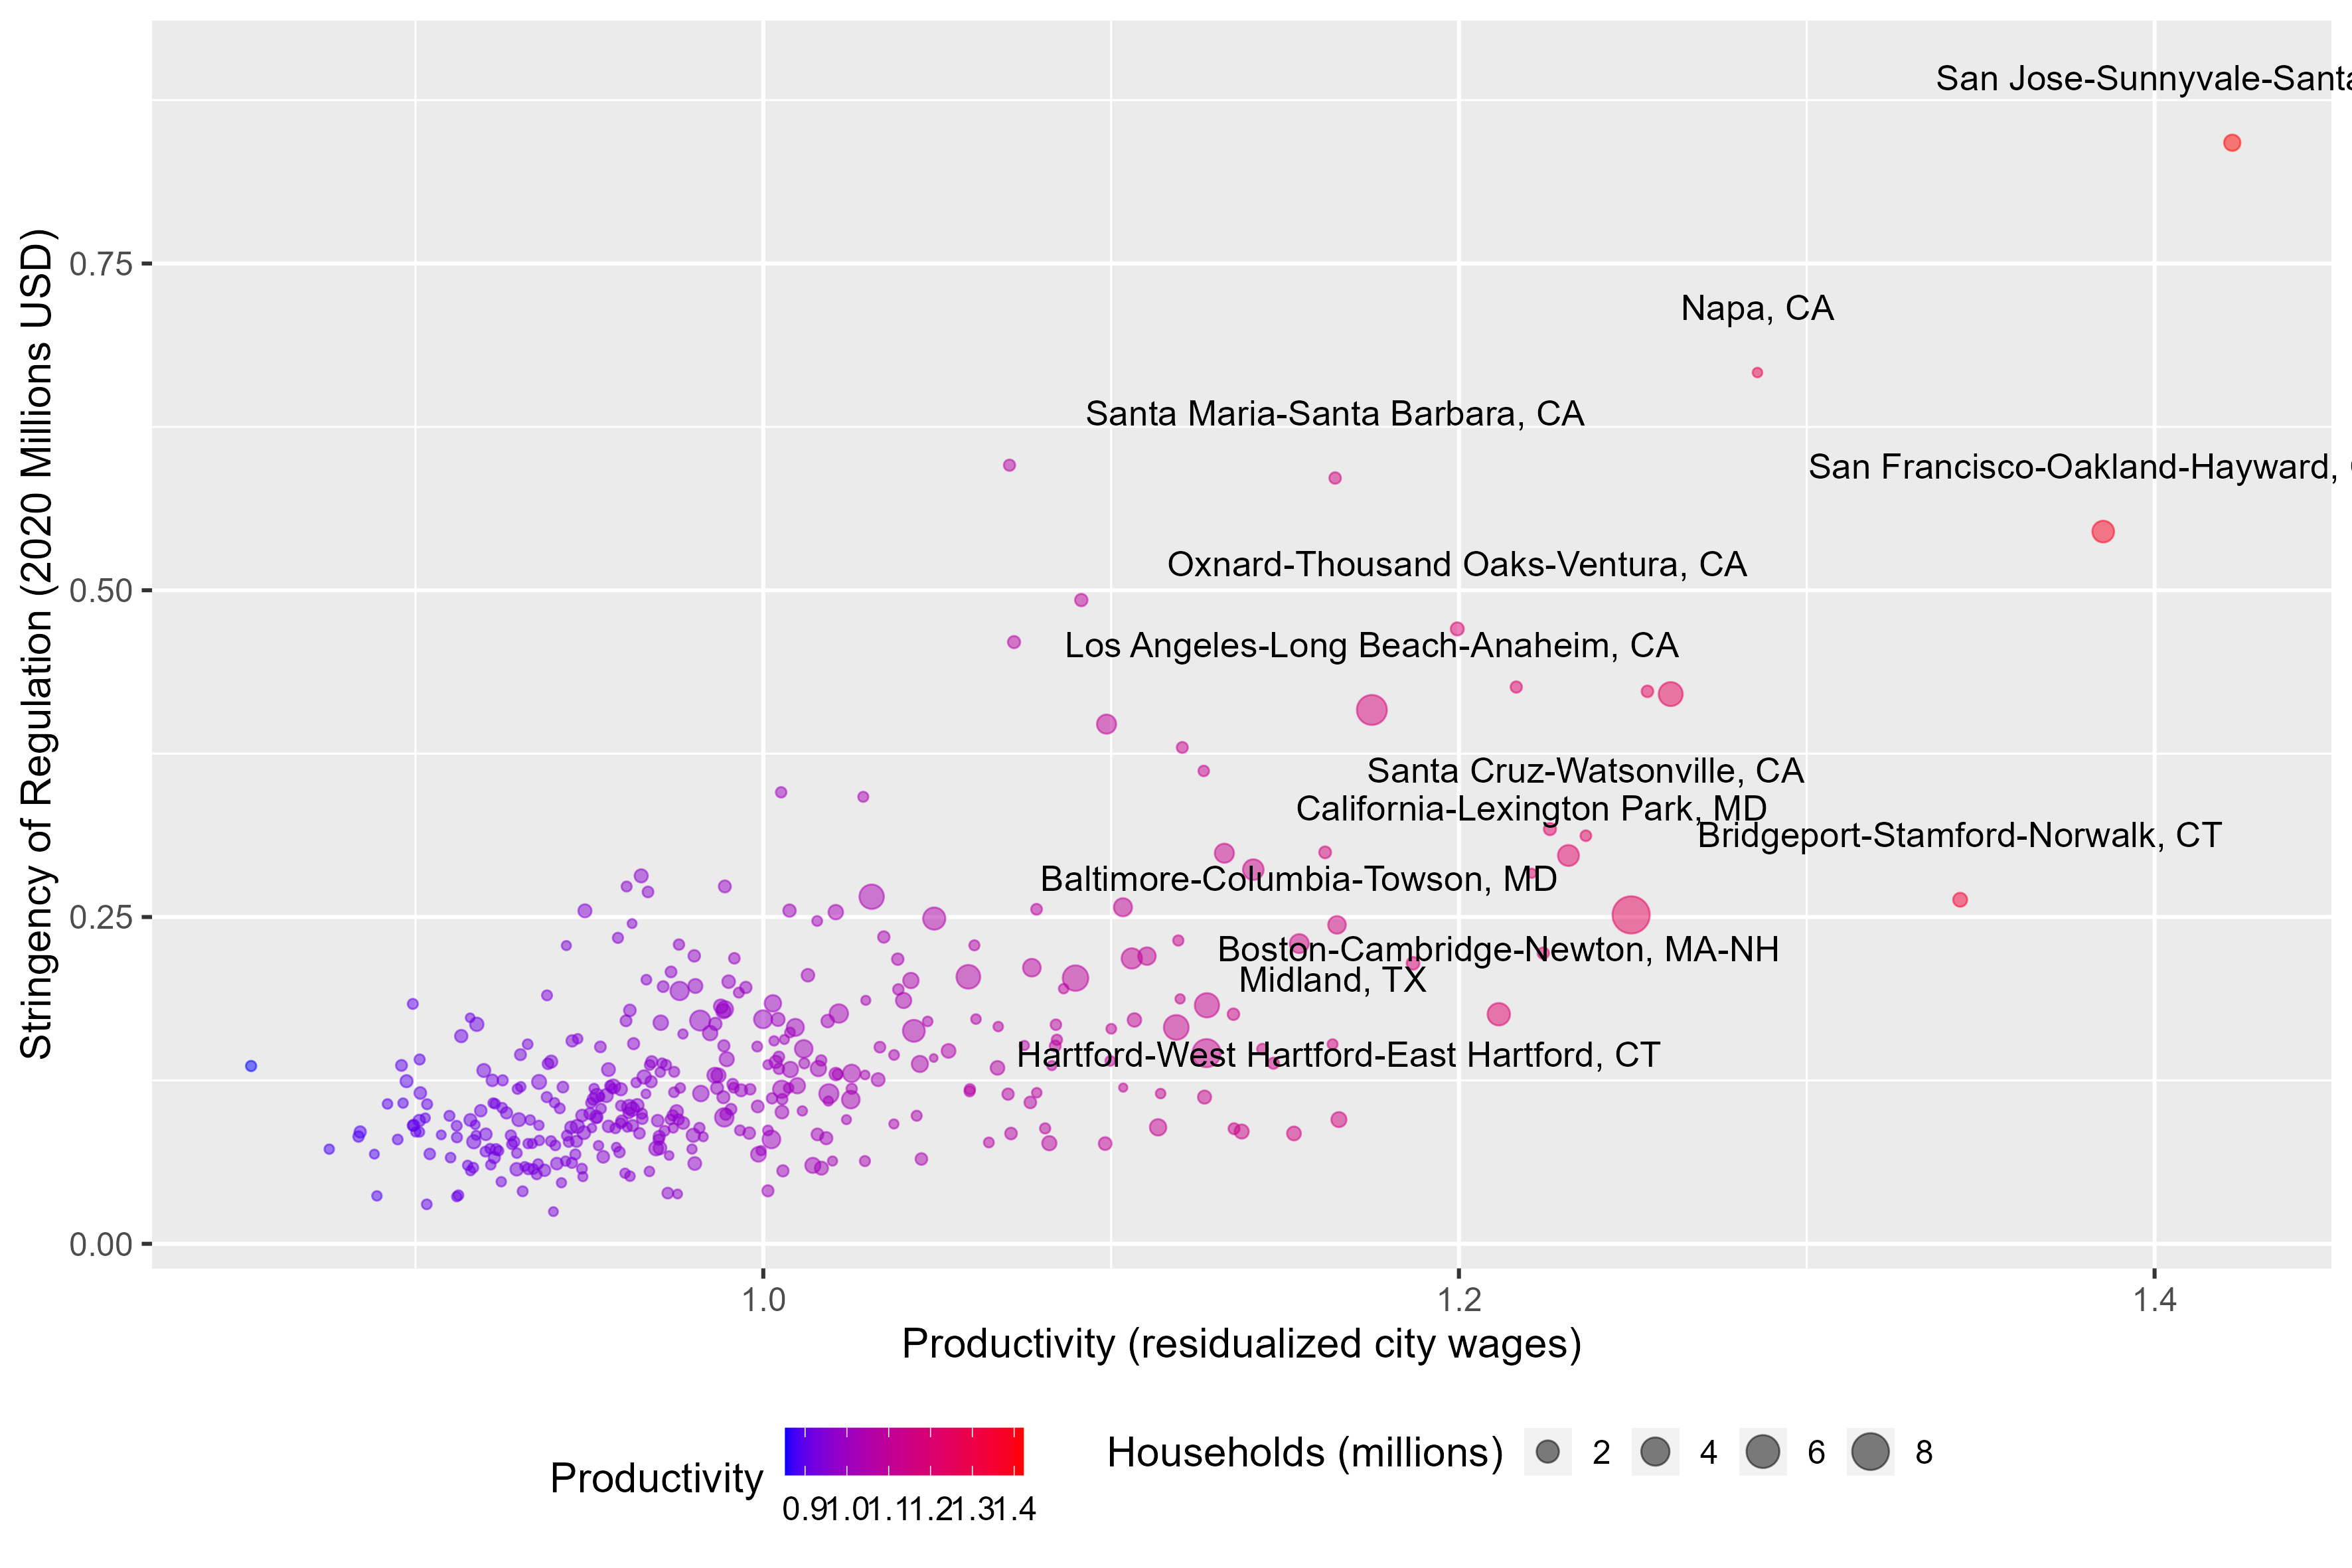
\includegraphics[width=1.1\textwidth]{ProductivityStringency.png}}
		\end{center}
		\caption*{Reports stringency measure introduced in Equation \eqref{observedStringency} plotted against residualized city wages with some additional city characteristics. For methodology behind construction of wages, see Section \ref{Section:CalibrationEstimation}. Productivity is normalized to be on average one across cities.}
	\end{table}
	
	
	
	
	\clearpage
	
	\subsection{Discussion of Alternative Specifications}\label{Appendix:Robustness}
	\paragraph*{}
	In this section, I provide additional robustness checks for the facts. I also discuss instances where Facts \ref{FIncomeDens} and \ref{FStringency} do not hold. 
	
	\paragraph*{Distance to CBD} Fact \ref{FIncomeDens} is not robust when considering distance to the CBD instead of the density ranking. In Figure \ref{figure:CBD_Facts}, I reproduce regressions of demeaned income (Panel A) and regulatory stringency (Panel B) on the distance to CBD. We observe a generally increasing relationship between income and CBD distance. Panel B shows that there is evidence that high density neighborhoods close to the CBD are less stringent in superstar cities. However, a key difference is that the relationship is not monotone for each city sample. 
	
	\begin{figure}[htbp!]
		\caption{Facts \ref{FIncomeDens} and \ref{FStringency} when considering distance to CBD}\label{figure:CBD_Facts}
		\makebox[\textwidth]{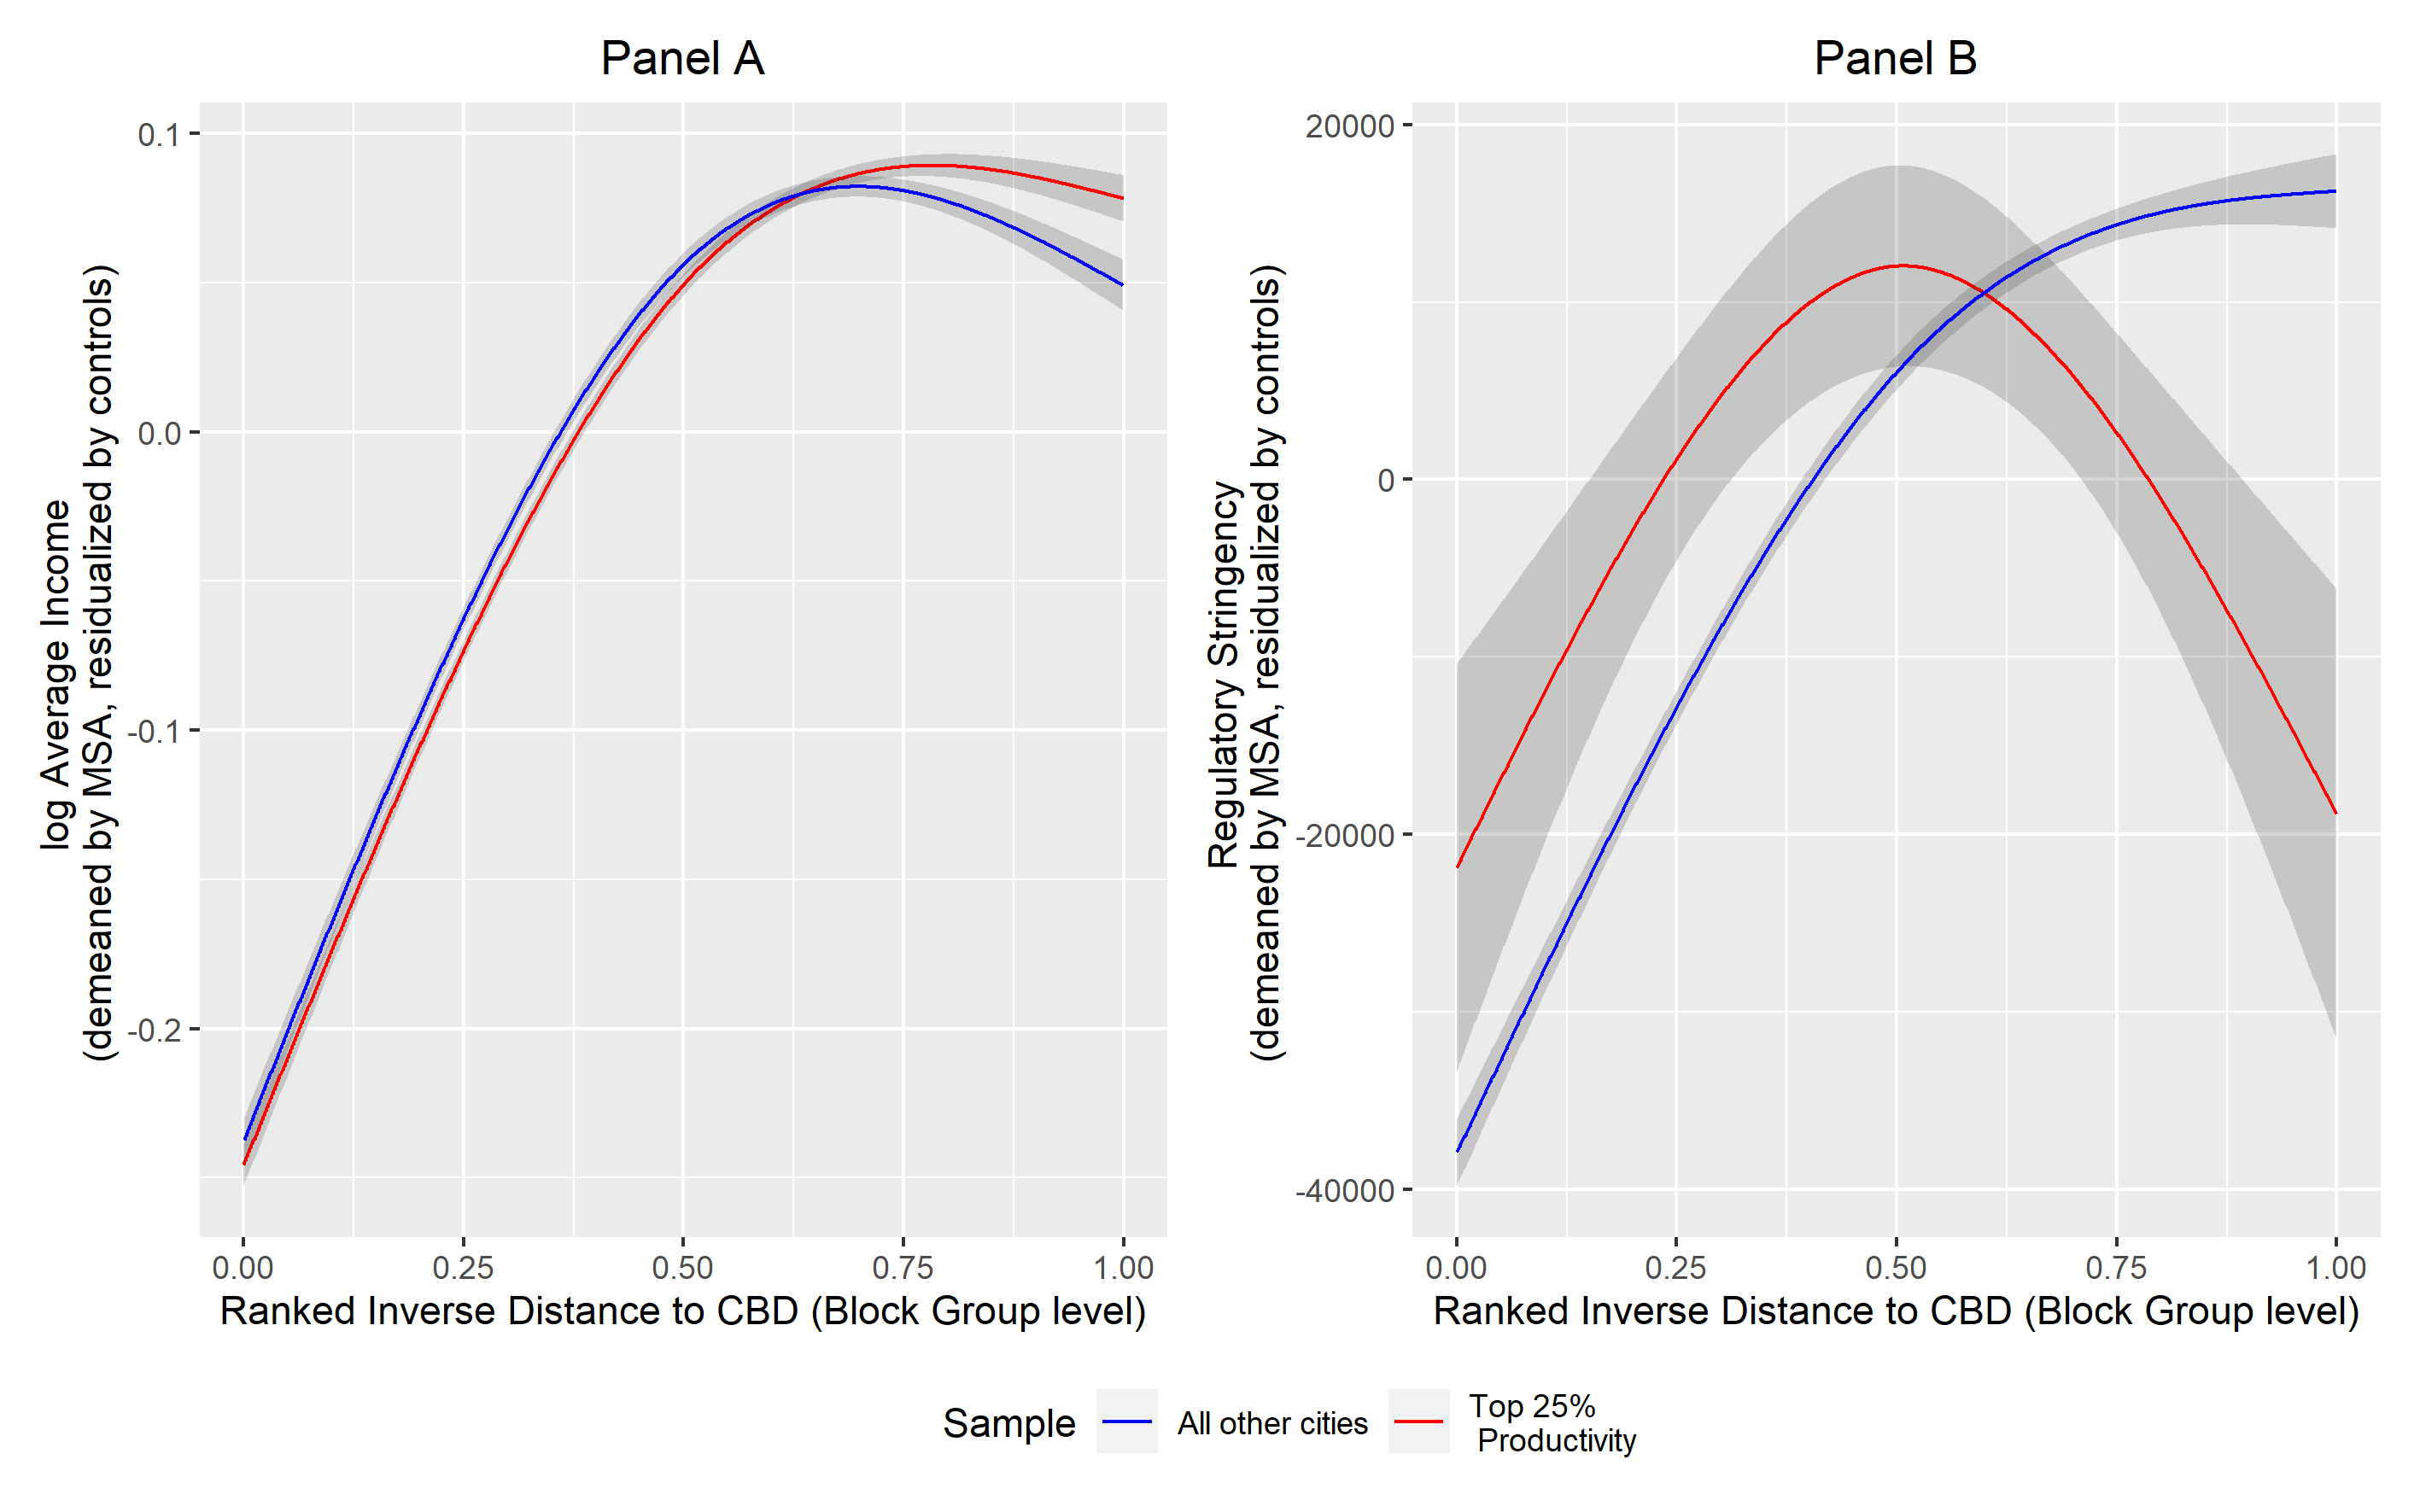
\includegraphics[width=1.1\textwidth]{CBD_combined.png}}
		
	\end{figure}
	
	
	\paragraph*{Relationship over time} Fact \ref{FIncomeDens} is robust to various time periods. I repeat the same exercise using 2008-2012 ACS data, with results reported in Figure \ref{figure:incSort_hist}. The difference in the negative income-density gradient across samples is somewhat stronger in this sample relative to the 2016-2020 ACS. This likely reflects the recent gentrification of high density neighborhoods nationwide. Results also hold when residualizing regressions by the standard set of controls. Unfortunately, my measure of regulation does not vary over time, and so Fact \ref{FStringency} cannot be checked historically. While there appears to be some recent adoption of minimum lot sizes between 2007-2020 \citep{gyourko2021},  there is probably little variation in regulatory stringency over time that could otherwise invalidate the relationship. 
	
	\begin{figure}[htbp!]
		\caption{Fact \ref{FIncomeDens} in 2008-2012 ACS sample}\label{figure:incSort_hist}
		\makebox[\textwidth]{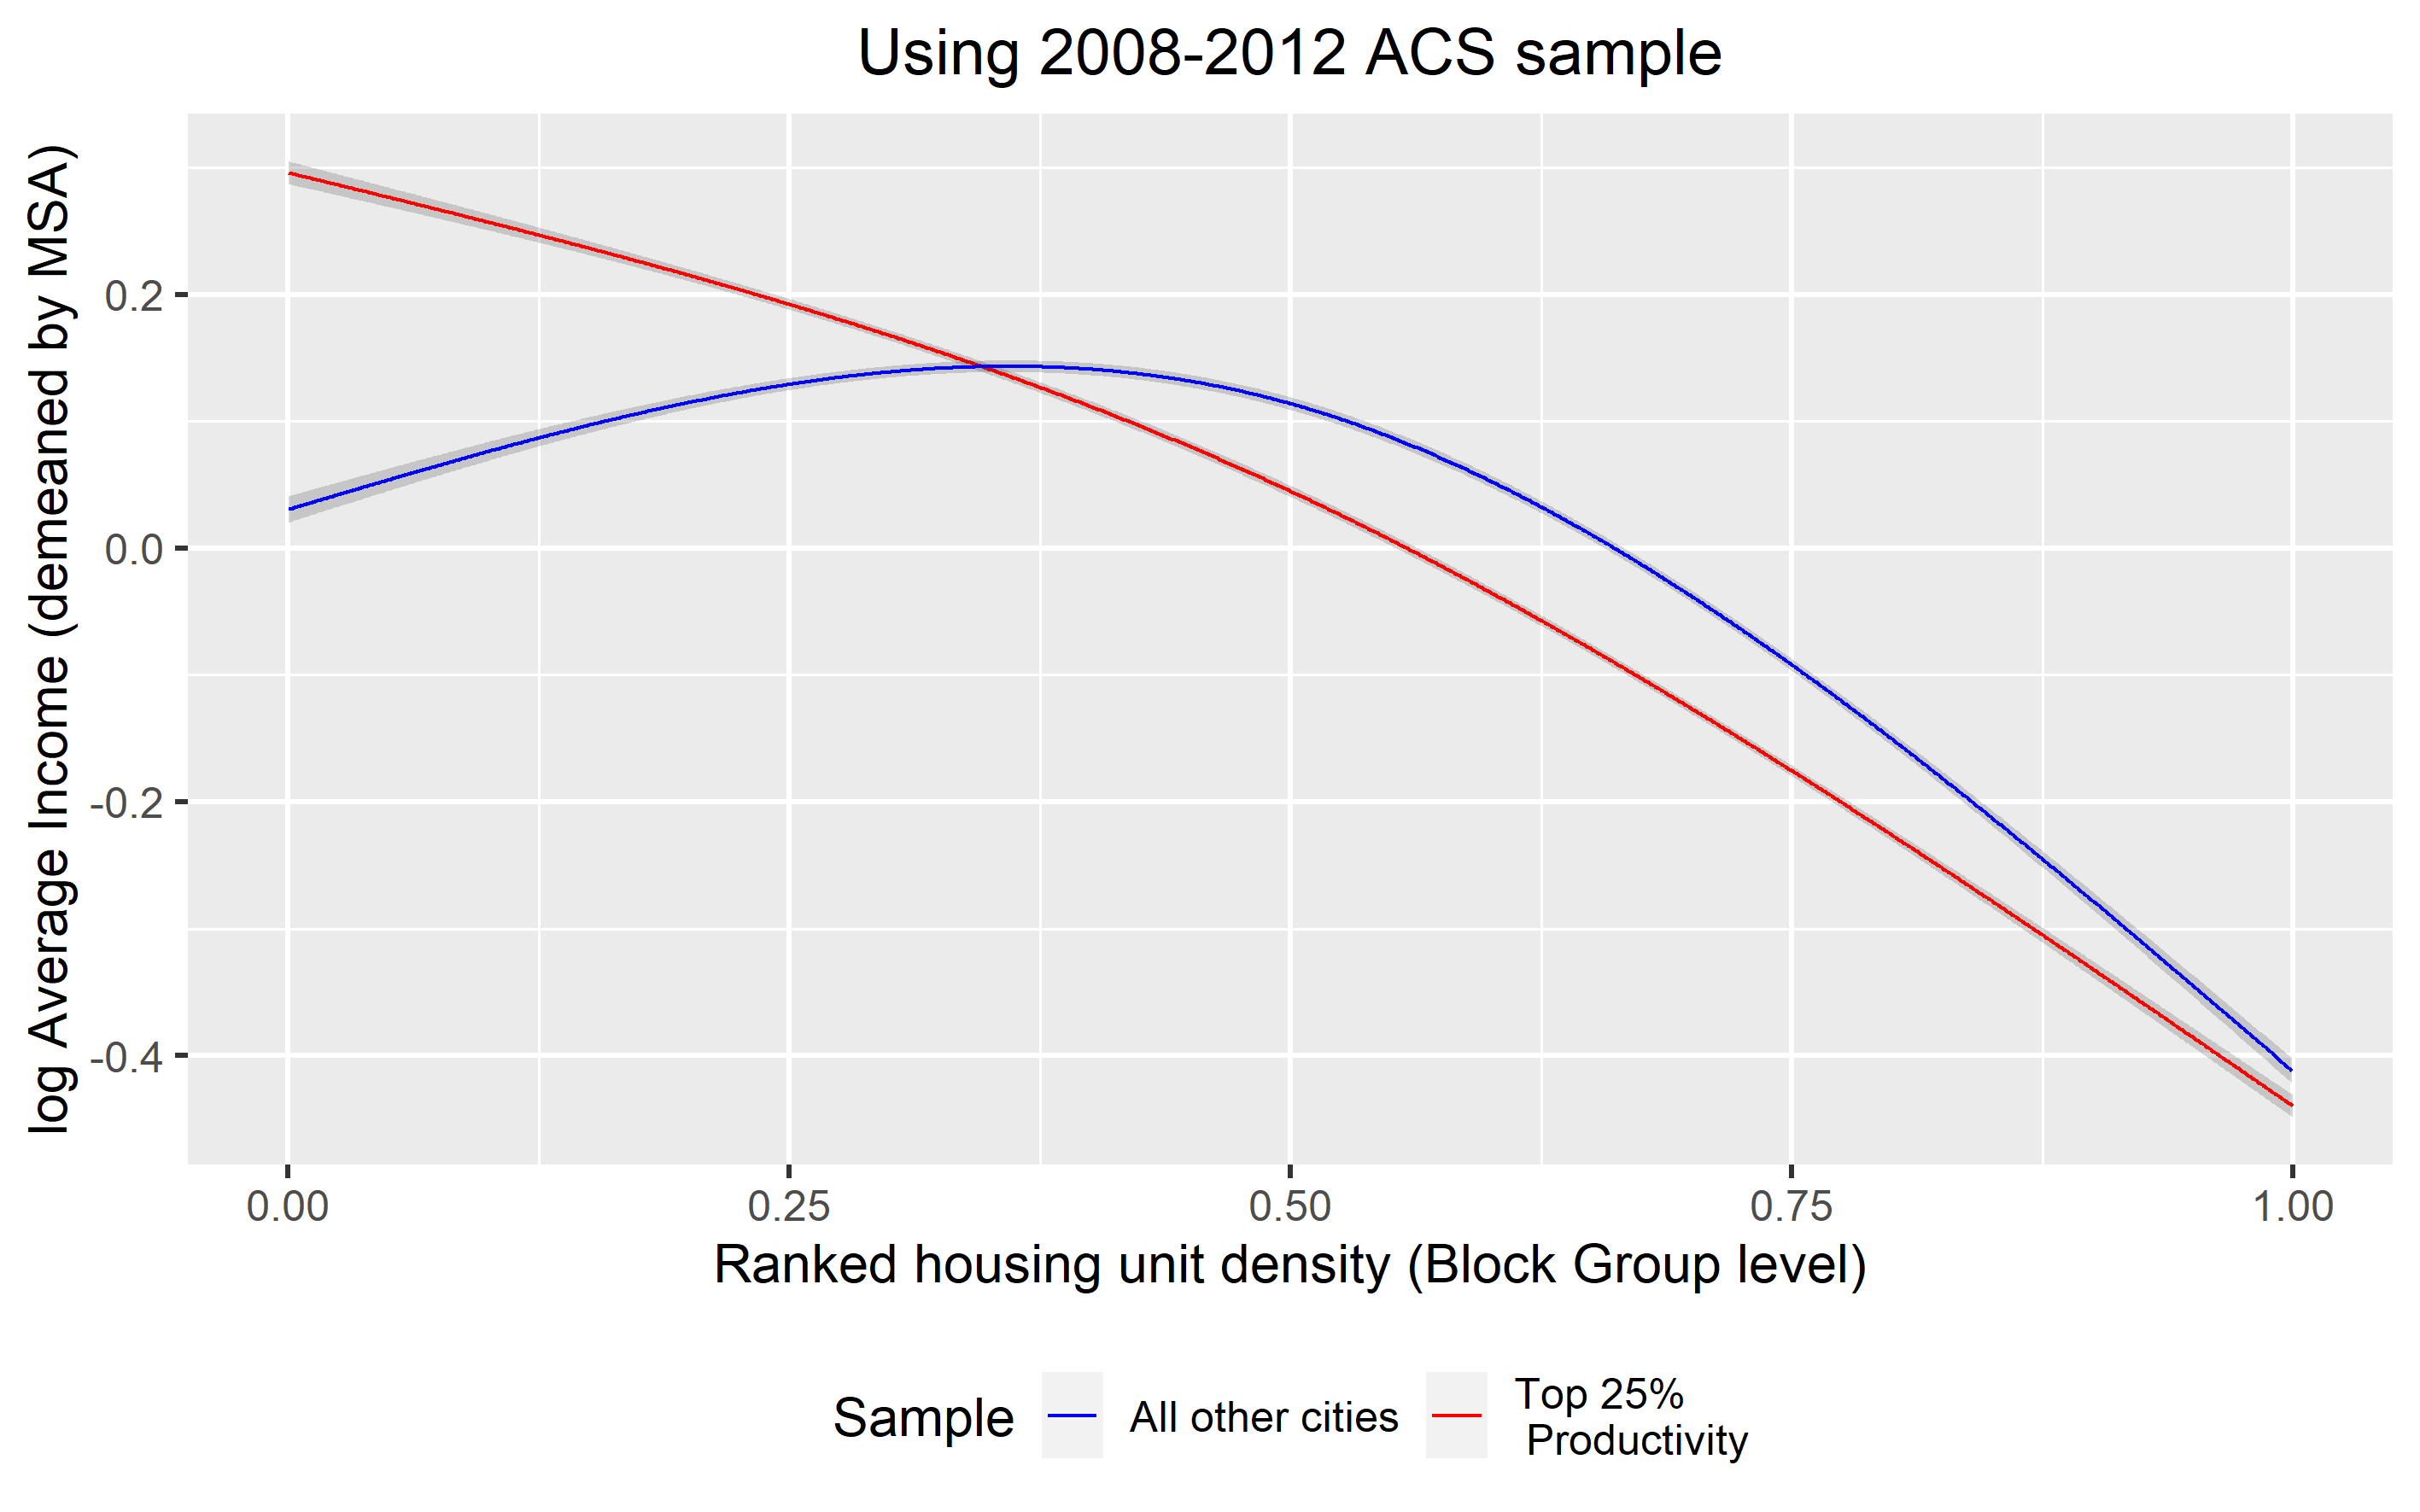
\includegraphics[width=0.9\textwidth]{income_2010.png}}
		
	\end{figure}
	
	\paragraph*{Alternative measures of superstars} Facts \ref{FIncomeDens} and \ref{FStringency} look quantitatively identical when adopting three different measures of "superstar" cities: the top $25\%$  and bottom  $75\%$ of density, housing prices, and a measure of city productivity alone (see Section \ref{Section:CalibrationEstimation} for details on productivity measurement). Moreover, these facts are robust to alternative measures of superstars that use $10 \%$ and $50 \%$ thresholds in their definition (rather than the baseline $25\%$).  
	
	\paragraph*{Weights} Facts \ref{FIncomeDens} and \ref{FStringency} use regressions that weigh block groups evenly, roughly corresponding to a population-weighted regression. Both \ref{FIncomeDens} and \ref{FStringency} are not driven by larger weights ascribed to bigger cities; they hold when each city receives equal weight. Each figure also looks identical when weighting the regression by the number of households in each block group.
	
	\paragraph*{Various hyperparameters} There are a large amount of hyperparameters that characterize zoning districts, and thus the measure of regulation used to show Fact \ref{FStringency}. Reassuringly, these facts look quantitatively identical for the entire hyperparameter space considered. This is likely driven by the fact that there are only minimal differences in clusters across hyperparameters (after all, two-thirds of all block groups are assigned regulation by populated zoning codes). 
	
	
	
	\clearpage 
	\section{Appendix: Theory}\label{TheoryAppendix}
	
	\subsection{Derivation of the distortion factor}\label{derive_distortion}
	\paragraph*{}
	For brevity, I drop zone and neighborhood subscripts for this derivation. I start with solving the households maximization problem, restated here:
	
	\begin{equation}
		V(z) := \max_{A, g} \underbrace{\kappa(z)\beta^{-\beta}(1-\beta)^{-(1-\beta)}(A - \bar{A})^{\beta}g^{1-\beta}}_{\text{Consumption value}} + \underbrace{\log b(z)}_{\text{Amenity value}}
	\end{equation} 
	subject to
	\begin{eqnarray*}
		PA \geq R \; \text{and} \\
		PA + g \leq wz
	\end{eqnarray*}
	It is instructive to first consider the case where $R = 0$ (or equivalently, when regulation is not binding). This problem has the well known solution (ignoring amenities as they do not matter for consumption decisions)
	
	\begin{equation*}
		V(z) = \kappa(z)wz\frac{(1 - \frac{P \bar{A}}{wz})}{P^{\beta}} 
	\end{equation*}
	with spending shares equal to 
	
	\begin{equation*}
		\beta + (1 - \beta)\frac{P \bar{A}}{wz}
	\end{equation*}
	This means that regulation $R$ is binding if and only if 
	\begin{equation*}
		\frac{R}{wz} > \beta + (1-\beta)\frac{P\bar{A}}{wz}
	\end{equation*} 
	If regulation is binding, consumption $g$ is $wz - R$ and housing consumption $A$ is $\frac{R}{P}$. Substituting this into the maximization problem above yields
	
	\begin{equation*}
		V(z) = \kappa(z)\beta^{-\beta}(1-\beta)^{-(1-\beta)}(R - P\bar{A})^{\beta}P^{-\beta}(wz - R)^{1-\beta}
	\end{equation*}
	
	
	
	\paragraph*{}
	Multiplying and dividing $V(z)$ by the value $wz(1 - \frac{P\bar{A}}{wz})$ and rearranging allows us to express this indirect utility as a product of the utility if minimum lot sizes were not binding and a distortion factor, as is suggested in the text:
	
	\begin{equation}\label{appendix:completeDistortionfactor}
		V(z) = \underbrace{k(z)wz\bigg[\frac{1-\frac{P\bar{A}}{wz}}{P^{\beta}}\bigg]}_{\text{Undistorted utility}} \underbrace{\bigg[\frac{\big(1 - \frac{R}{wz}\big)\big(1 - \frac{P\bar{A}}{wz}\big)^{-1}}{1-\beta}\bigg]^{1-\beta}\bigg[\frac{\big(R - P\bar{A}\big)\big(wz - P\bar{A}\big)^{-1}}{\beta}\bigg]^{\beta}}_{\text{Distortion Factor}}
	\end{equation}
	Assuming $\bar{A} = 0$ (Cobb-Douglas preferences), Equation \eqref{appendix:completeDistortionfactor} reduces down to what is reported in the text: 
	
	\begin{equation*}
	\underbrace{\kappa(z)\frac{w(i)z}{P_{R}(i)^{\beta}}}_{\text{Undistorted utility}}  \times \underbrace{\biggl[\frac{\frac{R(i)}{w(i)z}}{\beta}\biggl]^{\beta}\biggl[\frac{1- \frac{R(i)}{w(i)z}}{1-\beta}\biggl]^{1 - \beta}}_{\text{Distortion factor}}
	\end{equation*}
	where neighborhood and zone indicators are reintroduced in the equation for comparison.
	
	\clearpage
	\subsection{Derivation of Equation \eqref{supermodularity}}\label{derive_supermodularity} 
	
	\paragraph*{}
	Recall the household's problem \eqref{utility}, dropping neighborhood and zone subscripts. The objective is to prove that 
	\begin{equation}
		\frac{\partial}{\partial z}\bigg[\frac{\partial V(z)}{\partial R}/\frac{\partial V(z)}{\partial P}\bigg] < 0
	\end{equation}
	Whenever regulation is binding at $z$. To do this, we use the formula $V(z) = \kappa(z)\beta^{-\beta}(1-\beta)^{-(1-\beta)}(R - P\bar{A})^{\beta}P^{-\beta}(wz - R)^{1-\beta}$ from Appendix \ref{derive_distortion}. It can be easily shown that 
	
	\begin{equation*}
		\frac{\partial V(z)}{\partial R} = V(z)\bigg(\beta\frac{1}{R - P\bar{A}} - (1-\beta)\frac{1}{wz - R} \bigg)
	\end{equation*}
	and 
	\begin{equation*}
		\frac{\partial V(z)}{\partial P} = -V(z)\beta\bigg(\beta\frac{1}{P} + (1-\beta)\frac{\bar{A}}{R - P\bar{A}}  \bigg)
	\end{equation*}
	so that
	\begin{equation}
		\frac{\partial V(z)}{\partial R}/\frac{\partial V(z)}{\partial P} = -\frac{\beta\frac{1}{R - P\bar{A}} - (1-\beta)\frac{1}{wz - R} }{\beta\frac{1}{P} + (1-\beta)\frac{\bar{A}}{R - P\bar{A}} }
	\end{equation}
	Differentiating this expression with respect to $z$ yields 
	\begin{equation}
		\frac{\partial}{\partial z}\bigg[\frac{\partial V(z)}{\partial R}/\frac{\partial V(z)}{\partial P}\bigg] = -\bigg[\beta\frac{1}{P} + (1-\beta)\frac{\bar{A}}{R - P\bar{A}}\bigg]^{-1}(1-\beta)\frac{w}{wz - R}
	\end{equation}
	Since regulation is binding ($\frac{R}{wz} > \beta + (1 - \beta)\frac{P \bar{A}}{wz}$ from \ref{derive_distortion}) we know that $R > P\bar{A}$. Then, for all $wz > R$, the above expression is strictly negative.  This proves the result.
	
	\clearpage
	
	\subsection{Microfoundations for endogenous amenities channel}\label{microfoundations}
	
	\paragraph*{}
	In this section, I provide an approximate microfoundations for the relationship in Equation \eqref{endoamen}. I abstract away from different zones within a neighborhood $i$.

	\paragraph*{Local public goods financed through income taxes} Suppose each neighborhood implements a property tax rate $t(i)$ on the value of a home (in terms of numeraire consumption). The revenue from this tax is rebated equally to all residents. Let $S(i)$ be total spending on housing in neighborhood $i$ by all residents. The average value of a home (which is equal to average spending on a home) from the housing market clearing condition is $$\frac{S(i)}{L(i)}$$ where $L(i)$ is the neighborhood population and so the consumption rebate is $t_{i}\frac{S(i)}{L(i)}$ for each household irrespective of income. Suppose households amenity value $b(i, z)$ is a composite of the public good $K$ and fundamential amenities $\nu(i, z)$, or $b(i, z) = K^{\Omega(z)}\nu(i, z)$. Then provision of the public good $K$ is $t_{i}\frac{S(i)}{L(i)}$. Then, amenity values are $b(i, z) = t_{i}^{\Omega(z)}\bigg[\frac{S(i)}{L(i)}\bigg]^{\Omega(z)}\nu(i, z)$. When housing consumption is Cobb-Douglas and no minimum lot sizes are binding, this means that $S(i) = \beta Y(i)$, where $Y(i)$ is total income in neighborhood $i$. Putting this all together, $$b(i, z) = \beta^{\Omega(z)}t_{i}^{\Omega(z)}\bigg[\frac{Y(i)}{L(i)}\bigg]^{\Omega(z)}\nu(i, z)$$ where $\frac{Y(i)}{L(i)}$ property tax rate terms $t(i)^{\Omega(z)}$ and spending shares $\beta^{\Omega(z)}$ are absorbed into the fundamental amenities term $\nu(i, z)$ (if they can reasonably be taken as exogenous). Obviously, property tax rates are endogenous in the local public finance literature, and respond to the changing income composition of the neighborhood to facilitate Tiebout sorting \citep{calabresetal, ineffTiebout}. Since I take a broad view of this neighborhood choice externality and include many reasons for why it occurs, I abstract away from these specific concerns. 
	
	\paragraph*{Local love of variety and a disutility of density} Suppose preferences over housing is Cobb-Douglas ($\bar{A} = 0$) and suppose the amenity component can be written as $b(i, z) = c^{\Omega'(z)}L(i)^{-\Omega(z)}\nu(i, z)$ where $L(i)$ is the population of neighborhood $i$ and $c$ is a composite consumption good (separate from the numeraire) that is produced in a Dixit-Stiglitz style market with some elasticity of substitution over varieties $\sigma_{\text{Variety}}$. This Dixit-Stiglitz style market only operates within the neighborhood $i$ (these goods are untraded across neighborhoods). I assume each variety that comprises the consumption good has an equilibrium price of 1 (the numeraire).
	
	\paragraph*{}
	Let $S(i)$ be the total spending in neighborhood $i$ on the consumption good $c$. Then, the number of varieties is proportional to total spending. The utility value of an additional variety is then $S(i)^{\frac{\sigma_{\text{Variety}}}{\sigma_{\text{Variety}}} - 1}$. Hence, we can write 
	$$b(i, z) = S(i)^{\Omega'(z)\frac{\sigma_{\text{Variety}}}{\sigma_{\text{Variety}}-1}}L(i)^{-\Omega(z)}\nu(i,z)$$ Also note that preferences over the numeraire, housing and amenities can be described as (taking a log transformation) $$A^{\beta}g^{1-\beta} + \log b(i, z) = A^{\beta}g^{1-\beta} +  \Omega'(z)\log c - \Omega(z)\log L(i) + \log \nu(i, z) $$ so that preferences are quasilinear in amenities $b(i, z)$. Consider a consumers problem to choose spending to maximize utility over $A$, $g$ and $c$, assuming consumption $c$ has a price of 1. Spending on $c$ is then pinned down via the first order condition (assuming no corner solution) $$\Omega'(z)\frac{1}{c} = 1 \implies c = \Omega'(z)$$ Suppose $\Omega'(z) \propto z$. This means that $S(i)$ is proportional to total neighborhood income (and thus average income) in each neighborhood $i$\footnote{I empirically estimate a positive relationship between $\Omega(z)$ and $z$ in the data, though it is less-than-proportional to income. See Table \ref{table:baselineIV}. }. Let $Y(i)$ be this total neighborhood income, with $Y(i) = \alpha S(i)$ for some constant $\alpha$. Finally, $b(i, z)$ can be written as $b(i, z) = (\alpha Y(i))^{\Omega(z)}L(i)^{-\Omega(z)}\nu(i, z)$. If we assume $\Omega'(z)\frac{\sigma_{\text{Variety}}}{\sigma_{\text{Variety}} - 1} = \Omega(z)$, we can lastly write
	$$b(i, z) =  \big[\frac{Y(i)}{L(i)}\big]^{\Omega(z)}\tilde{\nu}(i, z)$$ where $\alpha$ is absorbed in the unobserved amenities component. $\frac{Y(i)}{L(i)}$ is average income in $i$.
	
	\clearpage
	\subsection{Proof of Proposition \ref{Prop:ReproduceFacts}}\label{Proof:ReproduceFacts}
	\paragraph*{}
	Proposition \ref{Prop:ReproduceFacts} has three parts. First, it says that cities with higher productivity are relatively more affluent because of variation in regulatory stringency. Second, it says that, within cities, neighborhoods that have higher regulatory stringency in equilibrium also have lower density. Thirdly, regulation generates a negative income-density gradient that is stronger in more productive cities. For this proof only, I adopt a separate index for cities and neighborhoods -- $c$ and $i$, respectively. In what follows, note that we assume a perfect mobility equilibrium for this proof and thus a spatial equilibrium is a set of allocations across neighborhoods $L(i, c, z)$ such that $V(i, c, z) \leq V(z)$ for some $V(z)$ and $V(i, c, z) < V(z) \implies L(i, c, z) = 0$ for all $(i, c)$ pairs. Also note that preferences are Cobb-Douglas, $\bar{A} = 0$ and $\Omega(z) = 0$ for every $z$, each neighborhood provides unit amenity value and has an identical production technology for housing. Lastly, recall that I make no distinction between regulated and unregulated zones to make the exposition as simple as necessary. 
	
	\paragraph*{}
	For simplicity, I assume $i$ and $c$ and $z$ are continuous which will directly imply all results on discrete space. For a location with regulatory stringency $R(i, c)$ that offers wage $w(c)$, let $s(i, c, z) := \frac{R(i, c)}{w(c)z}$. I start with two lemmas. The first lemma characterizes the bid rent curve -- the maximal rent willing to be paid to live in an arbitrary neighborhood offering wages $w$ and regulation levels $R$. 
	
	\begin{Lemma}
		The bid rent curve $\theta$ satisfies 
		$\theta(i, c, z) = V(z)^{-\frac{1}{\beta}}w(c)^{\frac{1}{\beta}}s(i, c, z)\big(1-s(i, c, z)\big)^{\frac{1 - \beta}{\beta}} $ if $s(i, c, z) \in [\beta, 1)$, $\theta(i, c, z) = V(z)^{-\frac{1}{\beta}}w(c)^{\frac{1}{\beta}}$ if $s(i, c, z) < \beta$. If $s(i, c, z) \geq 1$ then $\theta(i, c, z) = 0$
	\end{Lemma}
	\begin{proof}
		This follows directly from rearranging Equation \eqref{utilitydecomp} to determine what the price of housing services must be to rationalize utility $V(z)$ at wages $w$ and regulation $I$. In addition, recall that we set utility to zero if the price of a minimal lot exceeds income.  
	\end{proof}
	
	\paragraph*{}
	The second lemma says that the slope of the bid rent curve across cities is strictly increasing income, all else equal, which will eventually imply income sorting on regulation. This result is essentially implied by the supermodularity property of \eqref{supermodularity} combined with regulatory stringency increasing faster than wages in $c$. 
	
	\begin{Lemma}
		If $V(i, c, z) = V(z)$ then $\frac{\partial \theta}{\partial c}$ is strictly increasing in $z$ when $s(i, c, z) \in (\beta, 1)$ or is constant when $s(i, c, z) < \beta$ or $s(i, c, z) \geq 1$. 
	\end{Lemma}
	\begin{proof}
		 The slope of the bid rent curve when $\beta < s(I, w, z) < 1$ can be expressed as $$\frac{\partial \theta}{\partial c} = \theta(i, c, z)\bigg[\frac{1}{\beta}\frac{w'(c)}{w(c)} + \frac{\partial s}{\partial c}s(i, c, z)^{-1} - \frac{1 - \beta}{\beta}\frac{\partial s}{\partial c}(1 - s(i, c, z))^{-1}\bigg]$$
		
		 Recall that $s(i, c, z) = \frac{R(i, c)}{w(c)z} = \frac{\alpha(c)i}{w(c)z}$ which is strictly increasing in $c$ by one of the Proposition's assumptions. This can be used to show $\frac{\partial \theta}{\partial c}$ is increasing in $z$ using similar arguments from Appendix \ref{derive_supermodularity}. 
		 
		 \paragraph*{}
		 Lastly, if $s(i, c, z) < \beta$ then  $\theta(i, c, z) = V(z)^{-\frac{1}{\beta}}w(c)^{\frac{1}{\beta}}$ which is constant in $z$ because of the assumption $V(z) = \max_{i, c}V(i, c, z) =  \frac{w(c)}{P(i)^{\beta}}$. The case where $s(i, c, z) \geq 1$ is trivial.
		  
	\end{proof} 
	
	\paragraph*{}
	The third lemma deals with across-neighborhood comparisons of the bid rent function. 
	\begin{Lemma}
		If $V(i, c, z) = V(z)$ then $\frac{\partial \theta}{\partial i}$ is strictly increasing in $z$ when $s(i, c, z) \in (\beta, 1)$ or is constant when $s(i, c, z) < \beta$ or $s(i, c, z) \geq 1$. 
		
		\begin{proof}
			Follows directly from the derivation in Appendix \ref{derive_supermodularity}. 
		\end{proof}
	\end{Lemma}
	
	\paragraph*{}
	Using these three lemmas will help with proving the three statements in Proposition \ref{Prop:ReproduceFacts}.
	
	\begin{enumerate}
		\item High productivity cities are (weakly) more affluent: \\
		
		\begin{proof}
			Recall that there are two income types $z_{1} > z_{0}$. Fix any two cities $c_{0}$ and $c_{1}$ with $c_{0} < c_{1}$. This result can be shown if one can prove that, for all neighborhoods $i$ where the minimum lot size in either city is binding for at least one agent
			
			\begin{equation*}
			\text{If} \; L(i, c_{0}, z_{1}) > 0 \; \text{then} \; L(i, c_{1}, z_{1}) > 0 \; \text{and} \; L(i, c_{1}, z_{0}) = 0
			\end{equation*}
			
			I will prove this. $L(i, c_{0}, z_{1}) > 0$ implies that type $z_{1}$ can successfully bid in the neighborhood, so that $\theta(i, c_{0}, z_{1}) = \max_{z} \theta(i, c_{0}, z)$. Suppose for contradiction that $L(i, c_{1}, z_{1}) = 0$ or $L(i, c_{1}, z_{0}) > 0$. Then, in either case, $\theta(i, c_{1}, z_{0}) = \max_{z} \theta(i, c_{1}, z)$. But this is impossible, since Lemma 2\footnote{Since we assume the minimum lot size is binding for at least one agent \textit{and} not all agents observe the value of a minimal that exceeding income, Lemma 2 implies strict supermodularity.} and  $\theta(i, c_{0}, z_{1}) = \max_{z} \theta(i, c_{0}, z)$ implies that $\theta(i, c_{1}, z_{1}) > \theta(i, c_{1}, z_{0})$. 
			
		\end{proof}
		
		\item (Weakly) stronger income density gradient in productive cities. 
		
		\begin{proof}
			Fix two cities with $c_{0}  < c_{1}$. It is sufficient to show that, If $L(i_{1}, c_{0}, z_{1}) > 0$ and the minimum lot size is binding for at least one type in at least one city, then the following hold
			
			\begin{enumerate}
				\item $L(i_{1}, c_{1}, z_{1}) > 0, \; \text{and} \;  L(i_{1}, c_{1}, z_{0}) = 0 \; \text{with}$
				
				\item $L(i_{0}, c_{1}, z_{1}) = 0, \; \text{or} \;  L(i_{0}, c_{1}, z_{0}) > 0$ 
			\end{enumerate}
			
			I prove this. a) $L(i, c_{1}, z_{1}) > 0$ and $L(i, c_{1}, z_{0}) = 0$ follows from the same argument in the proof of Statement 1. 
			\paragraph*{}
			
			It remains to show $b)$. Suppose, for contradiction, that $L(i_{0}, c_{1}, z_{1}) > 0$ and $L(i_{0}, c_{1}, z_{0}) = 0$; that is, high income types strictly outbid low income in the low regulation neighborhood of the productive city. Then $\theta(i_{0}, c_{1}, z_{1}) > \theta(i_{0}, c_{1}, z_{0})$. However, this immediately implies that $\theta(i_{0}, c, z_{1}) > \theta(i_{0}, c, z_{0})$ for every $c$ because $i_{0}$ neighborhoods are unregulated and thus the bid rents have the same slopes across income types (Lemma 2). However, this also then implies $\theta(i_{1}, c, z_{1}) > \theta(i_{1}, c, z_{0})$ for all $c$ because Lemma 3 ensures that the slope of the bid rent across neighborhoods is nondecreasing in $z$. Hence, $z_{0}$ types are outbid from all neighborhoods and cities, which cannot be an equilibrium. 
			
		\end{proof}
		
		
			
		\item  The density of housing units is (weakly) decreasing in $i$. 
		
		\begin{proof}
			It is sufficient to fix a city $c$ and show for any $i_{0}$ and $i_{1}$ such that $i_{0} < i_{1}$, $\sum_{z}L(i_{1}, c, z) \leq \sum_{z}L(i_{0}, c, z)$\footnote{Recall that all neighborhoods have identical land mass.}. Since $\theta(i, c, z)$ is decreasing in $i$ (regulation decreases utility when binding, thus maximal rent willing to pay), we must have that the equilibrium rent curve $\theta(i, c) = \max_{z}\theta(i, c, z)$ is also decreasing in $i$. 
			
			\paragraph*{} I prove that this is only commesurate with a population that is decreasing in $i$. Lemma 3 ensures that there are (weakly) relatively more $z_{1}$ types in $i_{1}$, and, for both $z$ types, housing expenditure per capita is weakly larger in $i_{1}$ than $i_{0}$ (strict if regulation is binding). Suppose for contradiction that the population is higher in $i_{1}$. This \textit{must} imply that total housing expenditure in $i_{1}$ is strictly higher than $i_{0}$. This implies strictly higher rents in $i_{1}$ than $i_{0}$ because we assume they have the same production technology for housing, contradicting the fact that  $\theta(i, c) = \max_{z}\theta(i, c, z)$ is decreasing in $i$. 
			
		\end{proof}
		
	\end{enumerate}
	
	
	\clearpage
	
	
	
	%%%%%%%%%%%%%%%%%%
	\subsection{A simple model showing why income heterogeneity matters for aggregate productivity}\label{Appendix:SimpleModelHeteroProd}
	
	\paragraph*{}
	In this section, I provide a simple model to explain why the presence of income heterogeneity can attenuate the productivity benefits of deregulating productive cities. This model does not depend on assumptions about endogenous amenities, though they may exacerbate this attenuation effect. To this end, consider a \textit{productive city} indexed by $c$ and an \textit{outside option} indexed by $o$. The outside option (representing the entire US economy not including the city $c$) offers an exogenous wage $\iota_{o}$ per unit of skill and utility level $V_{0}z$, proportional to skill level $z$ (as is the case with the Cobb-Douglas utility function).  
	The city $c$ offers an exogenous wage $\iota(c) > \iota_{o}$, and households pay endogenous rents $P(c)$ to live in the city. Preferences are Cobb-Douglas with parameter $\beta$. Assume total land supply in the city is fixed at $T(c)$, and there is an exogenous density of one housing unit per unit of land (i.e. the housing supply elasticity is zero). 
	
	
	\paragraph*{}
	First, consider the case where this city has no minimum lot size regulation. Housing market clearing in city $c$ implies a unique price $P(c)$ such that 
	
	\begin{equation}
		\beta \sum_{z \in Z} \frac{[\frac{\iota(c)z}{P(c)^{\beta}}]^{\theta}}{[\frac{\iota(c)z}{P(c)^{\beta}}]^{\theta} + [V_{0}z]^{\theta}}zL(z) = P(c)T(c)
	\end{equation}
	where there are Frechet idiosyncratic preference shocks with migration elasticity $\theta$\footnote{This assumption deviates from Gumbel shocks and is not important for the exposition. In the model, I introduce Gumbel preferences to help the model rationalize location choices of households by which observed income cannot cover the costs to rent a minimal lot. } and $L(z)$ is the mass of $z$ households in the economy. The assumptions about Cobb-Douglas preferences mean that location choice fractions $\frac{[\frac{\iota(c)z}{P(c)^{\beta}}]^{\theta}}{[\frac{\iota(c)z}{P(c)^{\beta}}]^{\theta} + [V_{0}z]^{\theta}}$ are independent of skill $z$. That is, all skills choose the production city in the same proportion. This means that we can compare two models where the support of the skill distribution $Z$ differs in an unregulated equilibrium. In fact, equilibria under any skill distributions $L(z)$ with the same total skill levels $\sum_{z}zL(z)$ will have equivalent prices $P(c)$ and aggregate productivity (population-weighted average wages) given in equilibrium
	
	\begin{equation}
		f(c)\iota(c)\sum_{z}zL(z) + (1-f(c))\iota_{0}\sum_{z}zL(z)
	\end{equation}
	where $f(c)$ is the $z$-independent share of households who choose city $c$. This logic is is synthesized by the lemma:
	
	\begin{Lemma}
		Suppose the above assumptions hold and there is no regulation. Then, with any arbitrary skill distribution with the same total income $\sum_{z}zL(z)$ results in the same equilibrium prices and relative skill levels across cities. This implies that aggregate productivity is invariant to any of these distributions.
	\end{Lemma}
	
	\paragraph*{}
	Having established this, I seek to show that a regulated equilibrium in a model with skill dispersion exhibits higher aggregate productivity than a model with only one skill level. With the logic above, this implies that complete deregulation leads to smaller productivity growth with skill heterogeneity relative to a model with homogeneity, which is the goal of the exercise. To this end, compare two distinct aggregate skill distributions indexed by $L_{d}$ for $d \in \{0, 1\}$ with the following properties:
	
	\begin{eqnarray}
		\sum_{z \in Z}zL_{0}(z) = 	\sum_{z \in Z}zL_{1}(z) \quad \text{and} \\
		\sum_{z \in Z}L_{0}(z) = 	\sum_{z \in Z}L_{1}(z)
	\end{eqnarray}
	
	\paragraph*{}
	Next, assume $L_{0}(z)$ has a support over only one $z$ value (no income heterogeneity), and that $L_{1}(z)$ has skill heterogeneity (a support of size 2 or more). The idea is to compare $L_{1}(z)$ with $L_{2}(z)$. Let $l(c)$ be the physical minimum lot size in the city. This means that there is an effective cap on the population of $\frac{T(c)}{l(c)}$, with this cap being reached exactly if every household faces binding regulation in conjunction with housing market clearing. This leads to the following statement:
	
	\begin{Lemma}
		Suppose all assumptions above hold and $l(c)$ is sufficiently large. Then, aggregate productivity with under regulation $l(c)$ is higher in the economy with the skill distribution $L_{1}$ relative to $L_{0}$. 
	\end{Lemma}
	
	The proof relies on constructing an equilibrium with $l(c)$ large enough so that regulation binds for all skill levels in the support of both $L_{0}$ and $L_{1}$\footnote{Such a finite regulation level must exist for finite support of a skill distribution as an equilibrium outcome. }. In a high-regulation environment, this means that equilibrium populations are identical under these skill distributions and equal to this population cap. However, because of income sorting driven by regulation differences, there will be relatively more high skill people in city $c$ relative to low-skill people under distribution $L_{1}$. With the assumed similarities between distributions above, numeraire good output in city $c$ will be higher with skill dispersion relative to no skill dispersion, and thus the same holds for aggregate productivity. 
		
	\paragraph*{}
	Setting $l(c)$ large enough to bind all households is unlikely to be borne in the data. However, this is a sufficient condition and not a necessary one. The main takeaway is that, if regulation is highly binding, increased skill dispersion manifests through skill sorting into productive cities and does not cause changes to equilibrium city size (in terms of the number of households). 
	
	
	
	\clearpage
	\subsection{Proof of Proposition \ref{Prop:NeighborhoodChoiceExt}}\label{Proof:NeighborhoodChoiceExt}
	
	\paragraph*{}
	Before proceeding with the proof, I start with some preliminary definitions. I define $s(i, z) = \frac{R(i)}{wz}$ and $\text{Inc}(i)$ to be the average income in $i$. Utility of neighborhood $i$ for type $z$ is $$V(i, z) := \frac{w}{P(i)^{\beta}}\bigg[\frac{s(i, z)}{\beta}\bigg]^{\beta}\bigg[\frac{1 - s(i, z)}{1 - \beta}\bigg]^{1 - \beta} + \Omega(z)\log \text{Inc}(i) + \log \nu(i, z)$$ when $s(i, z) \in (\beta, 1)$ and $\frac{w}{P(i)^{\beta}} + \Omega(z)\log \text{Inc}(i) + \nu(i, z)$ in an equilibrium where regulation is nonbinding. For each statement, I consider an equilibrium that is non-binding for all income types, but marginal changes would induce binding regulation (the special case where $s(i, z) = \beta$ for some type $z$). With imperfect labour mobility ($\rho < \infty$), an interior\footnote{An interior equilibrium is one where all types live in all locations where fundamental amenities are strictly positive. } equilibrium in this model can be expressed as 
	\begin{equation}\label{AppendixEq:EquilibriumPropNCE}
		e^{V(i, z)}L(i, z)^{-\frac{1}{\rho}} = V(z)
	\end{equation}
	for some $V(z)$, and for every type $z$ and neighborhood $i$. $L(i, z)^{-\frac{1}{\rho}}$ governs the additional selection effect from the idiosyncratic taste shocks over neighborhoods, which unsurprisingly vanishes as the variance of the taste shocks goes to zero $(\rho \to \infty)$. 
	
	\paragraph*{}
	Lastly, recall that I assume $\Omega(z)$ is increasing in $z$, which is commensurate with the empirical evidence of Section \ref{Section:EstNeighborhoodChoice}. Also, I need to assume $\Omega(z)$ for every $z$ is sufficiently small so as to guarantee equilibrium uniqueness, which in turn allows for comparisons across equilibria of different model parameterizations to make sense\footnote{For $\Omega$ sufficiently small, the equilibrium is likely stable because the disutility of a marginal increase in rents for small changes in population dominates any endogenous amenity response that could occur. Obviously, this is not in line with the empirical evidence on unstable neighborhood preferences, e.g. \citep{davisetalracepref}. I ignore these concerns here.}.
	
	\begin{enumerate}
		%\item Statement 1: For an unregulated equilibrium, the variation in income across neighborhoods is strictly increasing in $t$. 
		
		%\begin{proof}
		% \item Fix any $t \in (0, 1)$ and consider how a marginal change in $t$ alters the equilibrium. Totally differentiating \eqref{AppendixEq:EquilibriumPropNCE} for an arbitrary $i$ and $z$ yields an equation governing changes in equilibrium:
		 
		% \begin{equation}\label{AppendixEq:EqChanges}
		% 	 \frac{\partial L(i, z)}{L(i, z)} = -\rho \beta \frac{w}{P(i)^{\beta}}\frac{\partial P(i)}{P(i)} + \rho\Omega(z) \frac{\partial \text{Inc}(i)}{\text{Inc}(i)} + \rho\frac{\partial \nu(i, z)}{\nu(i, z)}  - \rho \frac{\partial V(z)}{V(z)}
		% \end{equation}
		 
		% Define $\Delta \text{Inc} := \frac{\partial \text{Inc}(1)}{\text{Inc}(1)} - \frac{\partial \text{Inc}(0)}{\text{Inc}(0)}$, $\Delta C = -\beta\frac{w}{P(1)^{\beta}}\frac{\partial P(1)}{P(1)} + \beta\frac{w}{P(0)^{\beta}}\frac{\partial P(0)}{P(0)}$, and $\Delta \nu(z) := \frac{\partial \nu(1, z)}{\nu(1, z)} - \frac{\partial \nu(0, z)}{\nu(0, z)}$. The objective is to show that $\Delta \text{Inc} > 0$ in equilibrium, which means that neighborhood incomes diverge and thus segregation increases. Equation \eqref{AppendixEq:EqChanges} can be expressed using the following formula by substituting the definition of $\frac{\partial V(z)}{V(z)}$
		
		% \begin{equation}\label{AppendixEq:PopulationFormula}
		 	%\frac{\partial L(1, z)}{L(1, z)} = \rho[1 - \tilde{f}(1, z)]\big[ \Delta C + %\Omega(z)\Delta \text{Inc} + \Delta \nu(z) \big]
%		 \end{equation}
		 %where $\tilde{f}(i, z)$ is the fraction of type $z$ households who choose $i$. 
		 
		 %\paragraph*{}
		 %I use this formula extensively for the proof. Define $\Delta Y_{1} = \frac{\partial Y(1)}{Y(1)} =  \frac{\partial (\sum_{z}zL(1, z))}{\sum_{z}zL(1, z)}$, the total income growth in location $1$. Moreover, since preferences are Cobb-Douglas, we know that $\frac{\partial P(i)}{P(i)} = \frac{1}{1 + \epsilon}\frac{\partial Y(i)}{Y(i)}$ and so 
		 
%		 \begin{equation*}
%		 	\Delta C = -\frac{\beta}{1 + \epsilon}\frac{w}{P(1)^{\beta}}\frac{\partial Y(1)}{Y(1)} + \frac{\beta}{1 + \epsilon}\frac{w}{P(0)^{\beta}}\frac{\partial Y(0)}{Y(0)} = \tilde{c}\Delta Y_{1}
%		 \end{equation*}
%		 where $\tilde{c} = -\frac{\beta}{1 + \epsilon}\frac{w}{P(1)^{\beta}} - \frac{\beta}{1 + \epsilon}\frac{w}{P(0)^{\beta}}\frac{Y(1)}{Y(0)}$ and exploiting the fact that $\partial Y(1) = -\partial Y(0)$ (total income is exogenous because wages are exogenous). We know that $\tilde{c} < 0$. 
		
%		\paragraph*{}
%		 On the other hand, the using the definition of $\Delta I$, we have that  $\Delta \text{Inc} = \sum_{z}[o(1, z) - f(1, z)]\frac{\partial L(1, z)}{L(1, z)} - \sum_{z}[o(0, z) - f(0, z)]\frac{\partial L(0, z)}{L(0, z)}$, where $o(i, z)$ is the share of income in $i$ payed to $z$ households, and $f(i, z)$ is the fraction of households in $i$ who are type $z$. Using \eqref{AppendixEq:PopulationFormula}, this can be greatly simplified
		
%		 \begin{equation*}
%		 	\Delta \text{Inc} = \rho \sum_{z}\phi_{z}[\Delta C + \Omega(z) \Delta \text{Inc} + \Delta \nu(z)]
%		 \end{equation*}
%		 where $\phi_{z} = [o(1,z) - f(1, z)]\tilde{f}(0, z) + [o(0,z) - f(0, z)]\tilde{f}(1, z)$. Finally, this means (after some algebra and substituting in the above expression for $\Delta C$)
		 
%		 \begin{equation}\label{AppendixEq:IncomeEquilibrium}
%		 	\Delta \text{Inc} = \rho \sum_{z}\phi^{I}_{z}[\tilde{c} \Delta_{1} Y + \Delta \nu(z)]
%		 \end{equation}
%		 where $\phi^{I}_{iz} = \frac{\phi_{z}}{1 - \rho\sum_{z}\phi_{z}\Omega(z)}$. Assuming $\Omega(z)$ is sufficiently small for every $z$, one can easily show that $1 - \rho\sum_{z}\phi_{z}\Omega(z) > 0$ for any possible allocation of types in each neighborhood, which we assume thus far. 
		 
%		 \paragraph*{}
%		 Finally,  we know that, by the definition of $\Delta_{1}Y$, 
		 
%		 $$\Delta_{1}Y = \sum_{z}o(1, z)\frac{\partial L(1, z)}{L(1, z)}$$
		 
%		and hence, 
		 
%		 \begin{equation}
%		 	\Delta_{1}Y =  \rho \sum_{z}\phi^{L}_{z}[ \tilde{c} \Delta_{1} Y + \Omega(z) \Delta \text{Inc} +  \Delta \nu(z)]
%		 \end{equation}
%		with $\phi^{L}_{z} := o(1, z)(1 - \tilde{f}(1, z))$. Suppose that $\Delta \nu(z_{h}) = \frac{1}{1 - t}\frac{1}{\phi^{L}_{z_{h}}} > 0$ and $\Delta \nu(z_{l}) = -\frac{1}{1 - t}\frac{1}{\phi^{L}_{z_{l}}} < 0$ and $\Delta \nu(z_{m}) = 0$, which defines the parameterization functions $\kappa_{z}(t)$ defining how fundamental amenities vary by $t$\footnote{This parameterization of fundamental amenities is consistent with $\kappa_{z}(0) = 0$ and $\kappa_{z}(1) = 1$ for every $z$. The functions that achieves this are $\kappa_{z}(t) = e^{-\int^{1}_{t}\frac{1}{\phi^{L}_{z}(1 - \tilde{t})}\frac{1}{\tilde{t}}d\tilde{t}}$, which depend on equilibrium allocations as a function of $t$ and is continuous for $t \in (0, 1)$.}. Substituting in this parameterization into the equation above implies that
		
%		\begin{equation}\label{AppendixEq:PopulationEquilibrium}
%			\Delta_{1}Y =  \rho \sum_{z}\phi^{L}_{z}[ \tilde{c} \Delta_{1} Y + \Omega(z) \Delta \text{Inc}]
%		\end{equation}
%		That is, output in $i = 1$ (and thus $i = 0$) is not a function of changing fundamental amenities, which greatly simplifies the analysis. Equations \eqref{AppendixEq:IncomeEquilibrium} and \eqref{AppendixEq:PopulationEquilibrium} define a $2 \times 2$ linear system that can be used to solve for $\Delta \text{Inc}$ in equilibrium. This, in turn, means that 
		
%		\begin{equation*}
%			\Delta_{1}Y =  \rho \sum_{z}\phi^{L'}_{z}\Omega(z) \Delta \text{Inc}
%		\end{equation*}
		
%		for $\phi^{L'}_{z} := \frac{\phi^{L}_{z}}{1 - \rho\tilde{c}\sum_{z}\phi^{L}_{z}}$ which is strictly positive since $\phi^{L}_{z} > 0$ for all $z$ and $\tilde{c} < 0$. Finally, substituting this expression for equilibrium output into \eqref{AppendixEq:IncomeEquilibrium} and simplifying yields a closed form expression for $\Delta \text{Inc}$ in equilibrium 
		
%		\begin{equation}
%			\Delta \text{Inc} = \rho \sum_{z}\frac{\phi^{I}_{z}}{\phi^{L''}(z)} \Delta \nu(z)
%		\end{equation}
%		 where $\phi^{L''}(z) = 1 - \rho^{2}\tilde{c}\sum_{z}\phi^{I}_{z}\sum_{z'}\phi^{L'}_{z'}\Omega(z')$, which is also strictly positive for $\Omega(z)$ small in any equilibrium allocation.
		 
%		 \paragraph*{}
%		 To complete the proof, we need to show that $\Delta \text{Inc} > 0$. We know that $\phi^{I}_{z_{h}} > 0$ since the output share of the highest income types is always larger than their fraction of the population. Moreover, $\phi^{I}_{z_{l}} < 0$ for the opposite reason. Since $\Delta \nu(z_{h}) > 0$, $\Delta \nu(z_{h}) < 0$ and $\Delta \nu(z_{m}) = 0$, this is all sufficient to show that $\Delta \text{Inc} > 0$. Hence, neighborhood incomes diverge strictly in $t$. 
		 
%		\end{proof}
		
		\item Statement 1: \textbf{Inclusionary Zoning}: For the $t = 1$ economy, a small increase in regulation in $i = 1$ increases average income in all locations.
		
		\begin{proof}
		Recall that, at $t = 1$, we have $\nu(1, z_{l}) = 0$ and $\nu(0, z_{h}) = 0$, so these types are fixed in their respective neighborhoods. It is then sufficient to show that a marginal change in regulation in $i = 1$ that is \textit{just binding} for $z_{m}$ types, captured through changes in $I(1)$, causes a reallocation of these households from neighborhood $i = 1$ to $i = 0$. This must increase income in all neighborhoods. 
		
		\paragraph*{} I start with some preliminaries. Fix any $t \in (0, 1)$ and consider how a marginal change in $t$ alters the equilibrium, ignoring the direct effect of regulation. Totally differentiating \eqref{AppendixEq:EquilibriumPropNCE} for an arbitrary $i$ and $z$ yields an equation governing changes in equilibrium:
		
		 \begin{equation}\label{AppendixEq:EqChanges}
			 	 \frac{\partial L(i, z)}{L(i, z)} = -\rho \beta \frac{w}{P(i)^{\beta}}\frac{\partial P(i)}{P(i)} + \rho\Omega(z) \frac{\partial \text{Inc}(i)}{\text{Inc}(i)} + \rho\frac{\partial \nu(i, z)}{\nu(i, z)}  - \rho \frac{\partial V(z)}{V(z)}
		 \end{equation}
		
		 Define $\Delta \text{Inc} := \frac{\partial \text{Inc}(1)}{\text{Inc}(1)} - \frac{\partial \text{Inc}(0)}{\text{Inc}(0)}$, $\Delta C = -\beta\frac{w}{P(1)^{\beta}}\frac{\partial P(1)}{P(1)} + \beta\frac{w}{P(0)^{\beta}}\frac{\partial P(0)}{P(0)}$, and $\Delta \nu(z) := \frac{\partial \nu(1, z)}{\nu(1, z)} - \frac{\partial \nu(0, z)}{\nu(0, z)}$. Equation \eqref{AppendixEq:EqChanges} can be expressed using the following formula by substituting the definition of $\frac{\partial V(z)}{V(z)}$
		
		 \begin{equation}\label{AppendixEq:PopulationFormula}
			\frac{\partial L(1, z)}{L(1, z)} = \rho[1 - \tilde{f}(1, z)]\big[ \Delta C + \Omega(z)\Delta \text{Inc} + \Delta \nu(z) \big]
					 \end{equation}
		where $\tilde{f}(i, z)$ is the fraction of type $z$ households who choose $i$. 
		
		\paragraph*{}
		I use this formula extensively for the proof. Define $\Delta Y_{1} = \frac{\partial Y(1)}{Y(1)} =  \frac{\partial (\sum_{z}zL(1, z))}{\sum_{z}zL(1, z)}$, the total income growth in location $1$. Moreover, since preferences are Cobb-Douglas, we know that $\frac{\partial P(i)}{P(i)} = \frac{1}{1 + \epsilon}\frac{\partial Y(i)}{Y(i)}$ and so 
		
		   \begin{equation*}
					 	\Delta C = -\frac{\beta}{1 + \epsilon}\frac{w}{P(1)^{\beta}}\frac{\partial Y(1)}{Y(1)} + \frac{\beta}{1 + \epsilon}\frac{w}{P(0)^{\beta}}\frac{\partial Y(0)}{Y(0)} = \tilde{c}\Delta Y_{1}
			\end{equation*}
			where $\tilde{c} = -\frac{\beta}{1 + \epsilon}\frac{w}{P(1)^{\beta}} - \frac{\beta}{1 + \epsilon}\frac{w}{P(0)^{\beta}}\frac{Y(1)}{Y(0)}$ and exploiting the fact that $\partial Y(1) = -\partial Y(0)$ (total income is exogenous because wages are exogenous). We know that $\tilde{c} < 0$. 
			
			
			\paragraph*{}
			Consider how $z_{h}$ types move in response to a marginal increase in regulation in $i=1$ about an equilibrium that is just about binding for $z_{m}$ types (i.e. $s(i, z_{m}) = \beta$). Define $\Delta L = \frac{\partial L(1, z_{m})}{L(1, z_{m})}$. 
			
			\begin{equation*}
					\Delta L = \rho[1 - \tilde{f}(1, z_{m})]\big[ \Delta C + \Omega(z_{m})\Delta \text{Inc} \big]
			\end{equation*}
			where $\Delta C$ retains its definition as the relative log change in consumption values. $\Delta C$ must equal
			
			\begin{equation*}
				\Delta C = \tilde{c}\Delta_{1}Y + \frac{w}{P(1)^{\beta}}\partial D(1, z_{m})
			\end{equation*}
			
			where $D(1, z) = \bigg[\frac{s(i, z)}{\beta}\bigg]^{\beta}\bigg[\frac{1 - s(i, z)}{1 - \beta}\bigg]^{1 - \beta} $ is the \textit{distortion factor} due to regulation (which is changed by $I(1)$), as well as $\tilde{c}$ and $\Delta_{1}Y$ retaining their definition above. $D(1, z) = 1$ in an equilibrium where regulation is just binding ($s(i, z) = \beta$). The idea is to show $\Delta L < 0$, which will then imply that average incomes in both locations increase.
			
			\paragraph*{}
			 Using the definition of $\Delta \text{Inc}$ and the fact that $\partial L(i, z_{h}) = \partial L(i, z_{l}) = 0$,
			 
			 \begin{equation*}
			 	\Delta \text{Inc} = [o(1, z_{m}) - f(1, z_{m})]\frac{\partial L(1, z_{m})}{L(1, z_{m})} - [o(0, z_{m}) - f(0, z_{m})]\frac{\partial L(0, z_{m})}{L(0, z_{m})}
			 \end{equation*} 
			which means we can express $\Delta \text{Inc} = \tilde{I}\Delta L$ where $\tilde{I} = o(1, z_{m}) - f(1, z_{m}) + [o(0, z_{m}) - f(0, z_{m})]\frac{L(1, z_{m})}{L(0, z_{m})}$. Moreover, $\Delta_{1}Y = o(1, z_{m})\Delta L$ by definition. Putting this all together, the change in population in equilibrium can be solved:
			
			\begin{equation}\label{AppendixEq:EquilibriumPopMTypes}
					\Delta L = \rho[1 - \tilde{f}(1, z_{m})]\big[ \tilde{c}o(1, z_{m})\Delta L + \frac{w}{P(1)^{\beta}}\partial D(1, z_{m})  + \Omega(z_{m})\tilde{I}\Delta L \big]
			\end{equation}
			
			This simple linear equation can be solved in $\Delta L$. The sign of $\Delta L$ in equilibrium retains the same sign as $\frac{w}{P(1)^{\beta}}\partial D(1, z_{m}) < 0$ provided $1 - \rho(1-\tilde{f}(1, z_{m}))[\tilde{c}o(1, z_{m}) + \Omega(z_{m})\tilde{I}] > 0$, which is guaranteed for $\Omega(z_{m})$ small enough. Hence, $\Delta L < 0$. As a consequence, incomes in both locations increase, since $\frac{\partial \text{Inc}(i)}{\text{Inc}(i)} = [o(i, z_{m}) - f(i, z_{m})]\Delta L$, which is positive for $i = 1$ and for $i = 0$ because $z_{m}$ types are below average income in $i = 1$ and above average in $i = 0$.  
			
			
		\end{proof}
		
		
		\item Statement 2: \textbf{Exclusionary Zoning}: In the $t = 0$ economy, increasing regulation in any neighborhood(s) does not increase average income in all locations. Instead, average income across neighborhoods weighted by the population of $z_{h}$ types increases. 
		
		\begin{proof}
			I consider a marginal change in $R(i)$ in some neighborhood (without loss of generality assume it is $i = 1$, since both neighborhoods are identical at $t = 0$). This marginal change is around an equilibrium that is just binding for $z_{l}$ types, i.e. exactly at the point where $s(1, z_{l}) = \beta$. Using a similar set of equations derived in Statement 1, we can express equilibrium in terms of $\Delta_{1}Y$ and $\Delta \text{Inc}$ as follows:
			
			\begin{equation}\label{AppendixEq:IncomeEquilibriumtZero}
				\Delta \text{Inc} = \rho \sum_{z}\phi^{I}_{z}[\tilde{c} \Delta_{1} Y + \frac{w}{P(1)^{\beta}}\partial D(1, z_{l})1_{z = z_{l}}] 
			\end{equation}
			
			where $1_{z = z_{l}}$ is the indicator function if $z = z_{l}$, and $\phi^{I}_{z}$ is defined above. Moreover, since each neighborhood is the same in this equilibrium (that is, all types are split evenly across neighborhoods), then it is easy to show that $\sum_{z}\phi^{I}_{z} = 0$. This means that Equation \eqref{AppendixEq:IncomeEquilibriumtZero} can be expressed as 
			
			\begin{equation*}
				\Delta \text{Inc} = \rho\phi^{I}_{z_{l}}\frac{w}{P(1)^{\beta}}\partial D(1, z_{l}) > 0
			\end{equation*}
			
			since $\partial D(1, z_{l}) < 0$ and $\phi^{I}_{z_{l}} < 0$. Hence, neighborhood incomes are diverging for marginal changes in regulation. We can use this fact to show that $\frac{\partial \text{Inc}(1)}{\text{Inc}(1)} >0$ (and the opposite in $i= 0$), completing the proof. 
			
			\paragraph*{}
			$\frac{\partial \text{Inc}(1)}{\text{Inc}(1)}$ can be written as 
			
			\begin{equation*}
				\frac{\partial \text{Inc}(1)}{\text{Inc}(1)} = \rho \sum_{z}\kappa(z)[\tilde{c}\Delta_{1}Y + \Omega(z)\Delta \text{Inc} + \frac{w}{P(1)^{\beta}}\partial D(1, z_{l})]
			\end{equation*}
			
			where $\kappa(z) = [o(1, z) - f(1, z)[1-\tilde{f}(1, z)]$. $\kappa(z)$ also has the property that $\sum_{z}\kappa(z) = 0$ when neighborhoods are identical. Substituting in the derivation of $\Delta \text{Inc}$ above and simplifying yields
			
			\begin{equation*}
				\frac{\partial \text{Inc}(1)}{\text{Inc}(1)} = [\rho \sum_{z}\kappa(z)\Omega(z)][\rho\phi^{I}_{z_{l}}\frac{w}{P(1)^{\beta}}\partial D(1, z_{l})] + \rho\kappa(z_{l})\frac{w}{P(1)^{\beta}}\partial D(1, z_{l})
			\end{equation*} 
			
			both terms are strictly positive, since $\kappa(z_{h}) > 0$ and $\kappa(z_{l}) < 0$ (along with $\phi^{I}_{z_{l}}$), and $\Omega(z)$ is nondecreasing in $z$ (by assumption). Hence, we have that incomes in $1$ increase in response to regulation. Moreover, an identical expression can be derived for $\frac{\partial \text{Inc}(0)}{\text{Inc}(0)}$ to show that it is strictly negative. Hence, one neighborhood must increase in income and the other decrease. 
		
		\end{proof}
		
	\end{enumerate}
	
	 
	%\clearpage
	%\subsection{Examining the welfare and distributional consequences in the \\ $t = 0$ and $t = 1$ economies.}\label{Proof:WelfareDistConsequences}
	%\paragraph*{}
	%Proposition \ref{Prop:NeighborhoodChoiceExt} has two parts. First, if income sorting is strong, it says that imposing a marginal increase in a minimum lot size from an unregulated equilibrium in the rich neighborhood $i_{1}$ such that it is binding for type $z_{m}$ causes a Pareto improvement for all renters. Second, if income sorting is weak, it says that imposing a marginal increase in a minimum lot size from a symmetric unregulated equilibrium in the rich neighborhood $i_{1}$ makes the low income types worse off and all other types better off. In what follows, we define utility derived from neighborhood $i$ for type $z$ as $\tilde{V}(i, z) := e^{V(i, z)}b(i, z)$ and note that we assume a perfect mobility equilibrium (that is, in the limit where the migration elasticities $\theta$ and $\rho$ are infinite). This means that a spatial equilibrium is defined as a set of allocations $L(i, z)$ such that $\tilde{V}(i, z) \leq \tilde{V}(z)$ for some $\tilde{V}(z)$ and all $i$ such that $\tilde{V}(i, z) < \tilde{V}(z) \implies L(i, z) = 0$. 
	
	%\paragraph*{Inclusionary Zoning}
	
	% I start by showing that, under strong income sorting absent regulation, renters of all incomes can benefit. Consider a marginal change in the rent on a minimal lot $R(i)$ in $i_{1}$ around an unregulated equilibrium that causes regulation to be binding for $z_{m}$ types who may choose to live there, but not for $z_{h}$ types\footnote{This marginal change is possible because high income types $z_{h}$ have strictly higher income.}. I show that this marginal change induces population flows that are Pareto improving for all renters if and only if $k \Omega > \frac{\beta}{1 + \epsilon}$ for some $k > 0$ that may depend on endogenous objects in the unregulated equilibrium. The effect of this reallocation on utility offered in neighborhood $i_{0}$ for an arbitrary income type $z$ satisfies $$\partial \tilde{V}(i_{0}, z) = \tilde{V}(i_{0}, z)\bigg(V(i, z)\beta \partial \log P(i_{0}) + \Omega \partial \log Inc(i_{0}) \bigg)$$
  	%where $Inc(i)$ is defined as the average income in neighborhood $i$. This holds because we %assume preferences are Cobb-Douglas, or $\bar{A} = 0$ in Equation \eqref{utility}. We can decompose the expression above. Housing prices in equilibrium are isoelastic in total spending on housing (this can be derived easily by manipulating the housing market clearing condition noting that neighborhood $i_{0}$ is unregulated). This means that 
	%$$\partial \log P(i_{0}) = \frac{1}{1 + \epsilon}\partial \log Y(i_{0})$$	
	%where $Y(i)$ is total income in $i$, $\sum_{z}zL(i, z)$. Moreover, the expression for $\partial \log Y(i)$ satisfies $\partial \log Inc(i) = \partial \log Y(i) - \partial \log L(i)$ where $L(i)$ is total population $L(i) = \sum_{z}L(i, z)$. Combining these expressions gets us $$\partial \tilde{V}(i_{0}, z) = \tilde{V}(i_{0}, z)\bigg( (\Omega - V(i, z)\frac{\beta}{1 + \epsilon}) \partial \log Y(i_{0}) - \Omega \partial \log L(i_{0})  \bigg) $$
	
	%\paragraph*{}
	%We can break down this expression even further. We know that $\partial \log L(i_{0}) = \frac{\partial L(i_{0}, z_{m})}{L(i_{0})}$ and $\partial \log Y(i_{0}) = \frac{z_{m}\partial L(i_{0}, z_{m})}{Y(i_{0})}$ and can substitute this into the equation above. So, to show that $\partial \tilde{V}(i_{0}, z) > 0$ it suffices to show that $\tilde{V}(i, z) \geq 0$ and $$(\Omega - V(i, z)\frac{\beta}{1 + \epsilon}) z_{m}L(i_{0}) - \Omega Y(i_{0}) \geq 0$$ 
	%which is true if and only if $$k(z)\Omega \geq \frac{\beta}{1 + \epsilon}$$ where $k(z) := V(i, z)^{-1}(1 - \frac{Y(i_{0})}{z_{m}L(i_{0})})$. Note that $k(z) > 0$ for all $z$ since $Y(i_{0}) < z_{m}L(i_{0})$ at the initial unregulated equilibrium. Define $k := \max_{z}k(z)$. 
	
	%\paragraph*{}
	%I will use the derivation above as a lemma to complete the proof. If  $k\Omega \geq \frac{\beta}{1 + \epsilon}$ for the $k$ defined above, then reallocations of the middle income types to $i_{0}$ in transition to the new spatial equilibrium increase $\tilde{V}(i, z)$ for both types $z_{l}$ and $z_{m}$ agents who live in $i_{0}$. This is because $L(i_{0}, z) > 0$ in the new regulated equilibrium for $z \in \{z_{l}, z_{m}\}$, and so it must be the case that $\tilde{V}(i_{0}, z) = \max_{i}\tilde{V}(i, z)$ for each $z \in \{z_{l}, z_{m}\}$. Finally, we know that $\tilde{V}(i_{1}, z_{h})$ increases in transition to the new equilibrium because rents fall, average residential income increases and regulation is not binding for high types in $i_{1}$. Hence, we have that a marginal change in minimum lot sizes $\partial l$ induces changes in utility such that $$\partial \max_{i}\tilde{V}(i, z) \geq 0$$ for every income type $z$. Moreover, $\partial \max_{i}\tilde{V}(i, z_{h}) > 0$. This is the definition of a Pareto improvement (for renters only). 
	
	%\paragraph*{Exclusionary Zoning} I turn toward welfare analysis when fundamental amenities are equal for all types. Consider a marginal change in the rent on a minimal lot $R(i)$ in $i_{1}$ around the symmetric equilibrium that causes regulation to be binding for $z_{l}$ types who may choose to live there, but not for $z_{m}$ or $z_{h}$ types. A marginal change in populations by type $\partial L(i, z)$ is induced by this minimum lot size cause changes in welfare of those living in $i_{0}$ (via a similar calculation made in Statement 1) 
	%$$\partial \tilde{V}(i, z) = \tilde{V}(i, z)\bigg( (\Omega - V(i, z)\frac{\beta}{1 + \epsilon}) \partial \log Y(i) - \Omega \partial \log L(i)  \bigg) $$ with  $\partial \log L(i) = \frac{\sum_{z} \partial L(i, z)}{L(i)}$ and $\partial \log Y(i) = \frac{\sum_{z}z\partial L(i, z)}{Y(i)}$. Substituting this into the welfare expression gets us 
	%$$\partial \tilde{V}(i, z) = \tilde{V}(i, z)\sum_{z' \in Z}\bigg( (\Omega - V(i, z)\frac{\beta}{1 + \epsilon})z\partial L(i, z')Y(i)^{-1} - \Omega \partial L(i, z)L(i)^{-1}   \bigg) $$
	%fix any income type $z'$ and consider the expression $$(\Omega - V(i, z)\frac{\beta}{1 + %\epsilon})zY(i)^{-1} - \Omega L(i)^{-1}$$
	%which is positive (or negative) iff $$k(z)\Omega > \frac{\beta}{1 + \epsilon} \quad \text{or} %\quad k(z)\Omega <\frac{\beta}{1 + \epsilon} $$
	%with $k(z) := V(i, z)^{-1}(1 - \frac{Y(i)}{z'L(i)})$. This term is which is always negative %when $z' = z_{l}$ since $z_{l}L(i) < Y(i)$ for every $i$ ($l$ types are always below average income). Moreover, for $z' = z_{m}$ types are above the average income $\frac{Y(i)}{L(i)}$, then this term is positive provided $\Omega$ is large relative to the spending share on housing $\beta$ downweighted by the housing supply elasticity $\epsilon$. It is also then positive when $z' = z_{h}$. 
	%\paragraph*{}
	%Define $k = \max_{z \in \{z_{m}, z_{h}\}} k(z)$. Then regulation inducing the movement of low types to $i_{0}$ ($\partial L(i_{0}, z) < 0$) increases utility in $i_{1}$ and decreases in $i_{0}$ for both $z_{m}$ and $z_{h}$ types. To maintain spatial equilibrium, this requires that $\partial  L(i_{1}, z) > 0$ for both $z_{m}$ and $z_{h}$ types. These movements are commensurate with increasing utility in $i_{1}$ neighborhoods for middle and high income types, and decreasing utility in $i_{0}$ for low income types. In spatial equilibrium, we have 
	%\begin{eqnarray*}
	%	\partial \max_{i}V(i, z_{l}) < 0 \\
	%	\partial \max_{i}V(i, z_{m}) > 0 \\
%	\partial \max_{i}V(i, z_{h}) > 0
%	\end{eqnarray*}  
%	which completes the proof. 

	
	
	\clearpage
	
	\subsection{Social planning problem and proof of Proposition \ref{Prop:OptimalPolicy}}\label{Appendix:SocialPlanningModel}
	
	\paragraph*{}
	I start by restating the problem for convenience. The \textbf{Social planner's problem} for a set of household weights $\{\alpha(z)\}_{z \in Z}$ and absentee landowner weights $\alpha^{L}$ is defined as the choice of numeraire consumption allocations $g^{C}(i, z)$ and $g^{L}(i, z)$ for households and landowners respectively, housing consumption allocations $A(i, z)$, and total capital inputs into housing production $g^{A}(i)$, and welfare values $\boldsymbol{W}(z)$ to solve
	\begin{equation}
		\max   \sum_{z \in \boldsymbol{Z}}\alpha(z)\log \boldsymbol{W}(z) +\alpha^{L}\Pi
	\end{equation}
	where  $\Pi:= \sum_{i \in N}g^{L}(i)$ is the total numeraire consumption paid to landowners. Maximization is done subject to the following resource, free mobility and population balancing constraints:
	
	
	\begin{align}
		\sum_{i \in \cup_{c \in \mathbb{C}}N(c)}\big[\sum_{z \in Z}g^{C}(i, z)L(i, z)\big] + g^{A}(i) + g^{L}(i)& = & \underbrace{\sum_{c \in C}\bigg[\iota(c)\sum_{i \in N(c), z \in Z}zL(i, z) \bigg]}_{\text{Total production of numeraire}} \label{OptPolicy:BalancedGBudgetAppendix} \\
		\forall i, \; \; \sum_{z \in Z}A(i, z)L(i, z) & = & \underbrace{\lambda(i)^{\frac{1}{1 + \epsilon(i)}}g^{A}(i)^{\frac{\epsilon(i)}{1 + \epsilon(i)}}T(i)^{\frac{1}{1 + \epsilon(i)}}}_{\text{Local production of housing services}} \label{OptPolicy:BalancedHBudgetAppendix} \\
		\forall i, z,	\; \; V(i, z) - \frac{1}{\theta} \log \bigg[\frac{L(i, z)}{L(z)}\bigg]	 & = & \log \boldsymbol{W}(z) \label{OptPolicy:FreeMobilityAppendix} 	\\
		\forall z,	\; \;\sum_{i \in \cup_{c \in C}N(c)}L(i, z) & = & L(z) \label{OptPolicy:PopulationBalanceAppendix}
	\end{align}
	 where 
	 
	 \begin{equation*}
	 	V(i, z) = \kappa(z)(A(i, z) - \bar{A})^{\beta}\big[g(i, z)\big]^{1-\beta} + \Omega(z) \log \text{Inc}(i) + \log \nu(i, z)
	 \end{equation*}
	 In what follows, let $\Lambda^{C}$ be the lagrange multiplier for the constraint Equation \eqref{OptPolicy:BalancedGBudgetAppendix}, $\Lambda^{A}(i)$ for \eqref{OptPolicy:BalancedHBudgetAppendix},  $\Lambda^{FM}(i, z)$ for \eqref{OptPolicy:FreeMobilityAppendix} and $\Lambda^{L}(z)$ for \eqref{OptPolicy:PopulationBalanceAppendix}. In addition, let $V_{g}(i, z)$ and $V_{A}(i, z)$ be the marginal utility of numeraire and housing consumption, respectively, for a household of skill $z$ in neighborhood $i$. 
		
	\paragraph*{}
	For use with derivations,  I list important first order conditions associated with this problem:
	
		\begin{enumerate}
		\item FOC w.r.t $g^{C}(i, z)$ for fixed $z, i$
		
		\begin{equation}\label{Appendix:FOC_g}
			-\underbrace{\Lambda^{FM}(i, z)V_{g}(i, z)}_{\text{Weighted marginal utility of numeraire}}  = \Lambda^{C}L(i, z)
		\end{equation}
		
		\item FOC w.r.t. $L(i, z)$ 
		
		\begin{align}\label{Appendix:FOC_L}
			\begin{split}
			\sum_{z' \in Z}-\Lambda^{FM}(i, z')\Omega(z')\frac{\partial \log \text{Inc}(i)}{\partial L(i, z)} + \Lambda^{FM}(i, z)\frac{1}{\theta}\frac{1}{L(i, z)} + \Lambda^{C}\iota(i)z  = \\ \Lambda^{L}(z) + \Lambda^{C}g^{C}(i, z) + \Lambda^{A}(i)A(i, z)
			\end{split}
		\end{align}
	
		\item FOC w.r.t $A(i, z)$ for fixed $z, i$
		
		\begin{equation}\label{Appendix:FOC_A}
		-	\underbrace{\Lambda^{FM}(i, z)V_{A}(i, z)}_{\text{Weighted marginal utility of housing services}} = \Lambda^{A}(i)L(i, z)
		\end{equation}
		
		\item FOC w.r.t. $g^{A}(i)$ 
		\begin{equation}\label{Appendix:FOC_A_cap}
			\underbrace{ \tilde{\lambda}(i)\frac{\epsilon(i)}{1 + \epsilon(i)} \bigg[\frac{g^{A}(i)}{T(i)} \bigg]^{-\frac{1}{1 + \epsilon(i)}}}_{\text{Marginal product of capital in $i$'s housing sector }} = \frac{\Lambda^{C}}{\Lambda^{A}(i)}
		\end{equation}
		
	\end{enumerate}
	
	
	\paragraph*{}
	I emphasized two conditions that partially characterize the solution to this problem. 
	
	\paragraph*{Condition 1} The first condition concerns how a social planner trades off numeraire and housing consumption in each location:
	\begin{equation}\label{Equation:housingConsOpt_appendix_planner}
		\underbrace{\frac{V_{g}(i, z)}{V_{A}(i, z)}}_{\text{-MRS of housing for numeraire}} = 	\underbrace{\frac{\epsilon(i)}{1 + \epsilon(i)} \bigg[\frac{g^{A}(i)}{\lambda(i)T(i)} \bigg]^{-\frac{1}{1 + \epsilon(i)}}}_{\text{Marginal product of capital in $i$'s housing sector }}
	\end{equation}
	This is the standard MRS = MRTS condition that characterizes general equilibrium in the neoclassical model. This cannot be achieved with minimum lot size regulation because it necessarily distorts housing consumption for a given set of equilibrium prices, and more so for low income households.
	
	\paragraph*{}
	I use the first order conditions above to derive this equation. Rearranging and substituting Equation \eqref{Appendix:FOC_A} into Equation \eqref{Appendix:FOC_g} yields the following expression
	
	\begin{equation}\label{Appendix:MRS_lgrange_condition}
		\frac{V_{g}(i, z)}{V_{A}(i, z)} = \frac{\Lambda^{C}}{\Lambda^{A}(i)}
	\end{equation}
	
	and substituting Equation \eqref{Appendix:FOC_A_cap} into this yields the desired Condition 1.
	
	
	\paragraph*{Condition 2} The second concerns an efficient spatial allocation of households:
	
	\begin{equation}
		\sum_{z' \in Z}\Omega(z')\frac{\partial \log \text{Inc}(i)}{\partial L(i, z)}V_{g}(i, z')^{-1}L(i, z') + \iota(c)z - \frac{1}{\theta}V_{g}(i, z)^{-1}= \Xi(z) + g^{C}(i, z) + \frac{V_{A}(i, z)}{V_{g}(i, z)}A(i, z)
	\end{equation}
	for some constants $\Xi(z)$ I derive below. This equation ensures that the positive and negative externalities from amenity spillovers are balanced with aggregate productivity benefits of packing households in productive cities as well as the costs to the social planner to induce this movement. 
	
	\paragraph*{}
	I use the first order conditions to derive this. Substitute the expression for $\Lambda^{FM}(i, z)$ from Equation \eqref{Appendix:FOC_g} into Equation \eqref{Appendix:FOC_L}, as well as the expression for $\Lambda^{A}(i)$ from \eqref{Appendix:MRS_lgrange_condition} to get
	
	\begin{align}
		\begin{split}
			\Lambda^{C}\sum_{z' \in Z}\Omega(z')\frac{\partial \log \text{Inc}(i)}{\partial L(i, z)}V_{g}(i, z)^{-1}L(i, z) + -\Lambda^{C}\frac{1}{\theta}V_{g}(i, z)^{-1} + \Lambda^{C}\iota(i)z  = \\ \Lambda^{L}(z) + \Lambda^{C}g^{C}(i, z) + \Lambda^{C}\frac{V_{g}(i, z)}{V_{A}(i, z)}A(i, z)
		\end{split}
	\end{align}
	
	Divide both sides of the equality by $\Lambda^{C}$ to obtain
	
	\begin{align}
		\begin{split}
		\sum_{z' \in Z}\Omega(z')\frac{\partial \log \text{Inc}(i)}{\partial L(i, z)}V_{g}(i, z)^{-1}L(i, z) + -\frac{1}{\theta}V_{g}(i, z)^{-1} + \iota(i)z  = \\ 
		\frac{\Lambda^{L}(z)}{\Lambda^{C}} + g^{C}(i, z) + \frac{V_{g}(i, z)}{V_{A}(i, z)}A(i, z)
		\end{split}
	\end{align}
	
	and define $\Xi(z) := \frac{\Lambda^{L}(z)}{\Lambda^{C}}$, which completes the derivation.
	
	\clearpage
	
	
	\section{Appendix: Calibration}\label{Appendix:Calibration}	
	
	\subsection{The complete calibration algorithm}
	\paragraph*{}
	In this section, I detail the full algorithm that calibrates the model. I omit details of the calculations of hedonic prices, residualized wages, and other parameters because they are straightforward and explained with detail in Section \ref{Section:CalibrationEstimation}. This calibration starts with preference parameters $\beta$ and $\bar{A}$, which were calculated in a previously to match aggregate spending on housing for a random sample of $5,000$ block groups.  
	
	\begin{algorithm}
		\caption{Calibration}
		
		
			\begin{itemize}
			\item[] (Consumption values and supply parameters)
			\item[] For all block groups do
			
				\begin{enumerate}
					\item[] If Partially Regulated\footnote{}
					
					\begin{itemize}
						\item[] Uniquely solve equation \eqref{CalibrateUnregulated} for unregulated prices $P_{U}(i)$ given all other parameters, including regulated prices $P_{R}(i)$ and observed value of a minimal lot $R(i)$. Defines consumption value $C(i, z)$ and aggregate housing expenditure for each zone.
					\end{itemize}
					
					\item[]Else 
					
					\begin{itemize}
						\item[] Directly calculate $C(i, z)$ and housing expenditure given some housing price $P(i)$ and the value of a minimal lot $R(i)$. 
					\end{itemize}
									
				\end{enumerate}
				
				\begin{enumerate}
					\item[] If Fully or Partially Regulated
					\begin{itemize}
						\item[] Calculate $\lambda(i)$ to uniquely solve solve $\lambda(i)P_{R}(i)^{1 + \epsilon(i)}l(i) = R(i)$ for all partially or fully regulated block groups.
						
						\item[] Choose $T_{\boldsymbol{o}}(i)$ for each $\boldsymbol{o}$ to clear housing markets by zone. If Fully Regulated, $T_{\boldsymbol{U}}(i) = 0$.
						
					\end{itemize}
					
					\item[] Else
					\begin{itemize}
						\item[] Set $T_{U}(i)$ to some observed land mass of the block group and $T_{R}(i) = 0$. 
						
						\item[] Calculate $\lambda(i)$ to clear housing markets\footnote{}.
					\end{itemize}
					
					
				\end{enumerate}
				
				
	
			
			
			\item[] (Amenities)
			\item[] For all block groups do
			
			\begin{enumerate}
				\item  Choose amenities to uniquely solve \eqref{RosenRobackCalibrate} given $C(i, z)$ and populations $L(i, z)$ (up to a normalization) for each type. 
			\end{enumerate}
			
			
			\end{itemize}
		
		
	\end{algorithm}
	\footnotetext{A neighborhood is partially regulated if a block group is 1) assigned regulation previously, 2) has a positive fraction of housing units in regulated structures observed in the ACS, but this fraction is less than one. Fully regulated neigborhoods are identical to partially regulated neighborhoods except that the fraction of housing units in regulated structures is 1. Unregulated neighborhoods are all neighborhoods not satisfying one of the definitions above.}
	\footnotetext{In an unregulated neighborhood, $T_{R}(i)$ and $\lambda(i)$ are not separately identifiable parameters, so this allocation has no impact on counterfactual outcomes.}
	
		
	\clearpage
	\subsection{Calibration when households differ on education}\label{Appendix:CEdu}
	\paragraph*{}
	Extending the model to allow for households to differ by education requires some additional calibration methodology, which I detail here.
	
	\paragraph*{Wages by Education} Since households of differing education levels are not perfect substitutes in production (Equation \ref{prod_byskill}), they require a separate measure of wages. I regress log hourly wages in a set of occupation, sex, race, ancestry, year, quadratic in age and years of education, including MSA fixed effects separately for both college and non-college educated workers. These MSA fixed effects for both education groups form city and education specific wages per unit of effective labour, each normalized to be one in an average city. Productivity $\iota(c, s)$ by education $s$ is then derived to uniquely rationalize employment by education in each city and this city wage under the technology in Equation \eqref{prod_byskill} after specifying a value of $\sigma = 1.3$ \citep{card}.
	
	\paragraph*{Local education-skill distributions} The ACS block group tabulations do not report the joint distribution of households by skill $z$ and education status. I impute the joint distribution of neighborhood income and education by calculating the share of college workers by income type at the city level using the ACS microdata sample. I assume that this share by type applies uniformly over all neighborhoods within a given city. 
	
	\paragraph*{}
	All other calibration methodology when households differ on education is precisely the same as the baseline model where they do not (a type is redefined to be an income-education pair). I also assume that the support of the type distribution and spending shares on housing are the same across education levels within household income types. 
	
	
	\subsection{Summary Statistics for key calibrated parameters}\label{Appendix:CalibPara}
	
	\begin{landscape}
	\begin{table}[h]
		\caption{Summary Statistics for Key Calibrated Parameters, \\ disaggregated by SuperStar city sample}\label{table:CalibParaSuperstar}
		\makebox[\linewidth]{\resizebox{\textwidth}{!}{
\begin{tabular}{lrrrrrrrr}
\hline
\hline
SuperStar city & \multicolumn{4}{c}{No} & \multicolumn{4}{c}{Yes}  \\ 
 Variable & \multicolumn{1}{c}{N} & \multicolumn{1}{c}{Mean} & \multicolumn{1}{c}{Sd} & \multicolumn{1}{c}{Median} & \multicolumn{1}{c}{N} & \multicolumn{1}{c}{Mean} & \multicolumn{1}{c}{Sd} & \multicolumn{1}{c}{Median} \\ 
\hline
Housing price (Regulated zone) & 117078 & 0.58 & 0.4 & 0.49 & 76727 & 1.6 & 1.4 & 1.2 \\ 
Housing price (Unregulated zone) & 117078 & 0.87 & 0.91 & 0.6 & 76727 & 2.2 & 2 & 1.5 \\ 
\hline
ln Amenity value (0-25k) & 116199 & -0.093 & 0.19 & -0.09 & 75512 & 0.11 & 0.21 & 0.11 \\ 
ln Amenity value (25-50k) & 116199 & -0.075 & 0.18 & -0.074 & 75512 & 0.09 & 0.2 & 0.086 \\ 
ln Amenity value (50-75k) & 115939 & -0.08 & 0.19 & -0.073 & 75917 & 0.091 & 0.2 & 0.086 \\ 
ln Amenity value (75-100k) & 115939 & -0.086 & 0.2 & -0.075 & 75917 & 0.096 & 0.21 & 0.093 \\ 
ln Amenity value (100-150k) & 110697 & -0.075 & 0.22 & -0.062 & 75218 & 0.14 & 0.21 & 0.15 \\ 
ln Amenity value (150-200k) & 110697 & -0.087 & 0.23 & -0.079 & 75218 & 0.15 & 0.21 & 0.16 \\ 
ln Amenity value (200k+) & 110697 & -0.1 & 0.24 & -0.1 & 75218 & 0.17 & 0.23 & 0.17 \\ 
\hline
Consumption value (0-25k) & 117078 & 0.23 & 0.099 & 0.26 & 76727 & 0.16 & 0.12 & 0.19 \\ 
Consumption value (25-50k) & 117078 & 0.46 & 0.082 & 0.47 & 76727 & 0.42 & 0.14 & 0.46 \\ 
Consumption value (50-75k) & 117078 & 0.71 & 0.077 & 0.72 & 76727 & 0.7 & 0.15 & 0.73 \\ 
Consumption value (75-100k) & 117078 & 0.94 & 0.079 & 0.94 & 76727 & 0.95 & 0.15 & 0.98 \\ 
Consumption value (100-150k) & 117078 & 1.2 & 0.084 & 1.2 & 76727 & 1.2 & 0.14 & 1.2 \\ 
Consumption value (150-200k) & 117078 & 1.3 & 0.087 & 1.3 & 76727 & 1.4 & 0.13 & 1.4 \\ 
Consumption value (200k+) & 117078 & 1.4 & 0.088 & 1.4 & 76727 & 1.5 & 0.11 & 1.5\\ 
\hline
\hline
\end{tabular}
}


}
		\caption*{Summary statistics for calibrated (and estimated) housing prices, consumption values, and amenity values by income type. These statistics are broken down by the SuperStar and non-SuperStar sample used to construct Facts \ref{FIncomeDens} and \ref{FStringency} (top quartile of density and ACS reported housing prices). They are also reported for the entire sample. Amenity values $b(i, z)$ are normalized to have a mean of 1 (in levels, not logs). Differences in observation counts for amenity values are in block groups with no counts of the corresponding type. Consumption values $C(i, z)$ are rescaled so that they have the same standard deviation as a log Cobb-Douglas index with housing expenditure parameter $\beta = 0.2$.}
	\end{table}
	\end{landscape}

	
	\section{Appendix: Estimating $\Omega(z)$}\label{Appendix:Estimation}
	
	\subsection{Econometric model}\label{Appendix:EconometricModel}
	\paragraph*{}
	In this section, I specify a data generating process that justifies the use of the donut instrument to estimate each $\Omega(z)$. Consider a closed city with $N$ neighborhoods; these constitute the observed data. The structural equation for amenity value is, as in Equation \eqref{omega_estimation},
	
	\begin{equation*}
		\log b(i, z) = \Omega(z) \log \text{Inc}(i) + \beta_{1}(z)S\big[d_{1}(i)\big] + \log \nu(i, z)
	\end{equation*}
	where neighborhood income is determined by the neighborhood choice equation \eqref{laboursupply} subject to prices clearing housing markets. I specify that fundamental amenities $\log \nu(i, z)$ are a sum of two components:
	
	\begin{equation*}
		\log \nu(i, z) = \underbrace{\Upsilon(i,z)}_{\text{Unobserved demand factors}} +  \underbrace{\xi(i, z)}_{\text{Noise}}
	\end{equation*}
	where $\xi(i, z)$ is random noise that may be spatially correlated. $\Upsilon(i, z)$ contain unobserved demand factors that are not themselves slopes but can be correlated with slopes, i.e. weather, climate, views and ecetera. Note that if there were no unobserved demand factors\footnote{That is, $\Upsilon(i, z) = 0$ with probability $1$ for every $i$ and $z$.}, an instrument is still required because $\text{Inc}(i)$ will be endogenously determined by the shocks $\xi(i, z)$.  
	
	\paragraph*{}
	I allow for slopes in the buffer region to be cause unobserved local demand factors (or be correlated through some underlying latent variable). Structurally,
	
	\begin{equation}\label{Appendix:Slopes_and_demand_factors}
		\Upsilon(i,z) = \tilde{\gamma}(z)S\big[d_{1}(i)\big] + \sigma(i, z)
	\end{equation}
	for some $\sigma(i, z)$ capturing other demand unobservables orthogonal to slopes in the buffer region $d_{1}$. This term may have arbitrary spatial correlation. The identification assumption is that slopes outside the buffer region cannot be correlated with any unobserved demand factors, or
	
	\begin{equation}
		S\big[d_{2}(i)\big] \; \perp \; \sigma(i, z)
	\end{equation}
	which in turn requires that $S\big[d_{2}(i)\big]$ be "excluded" as a demand factor in Equation \eqref{Appendix:Slopes_and_demand_factors}. That is, slopes outside of the buffer cannot provide any additional information to predict unobserved demand factors beyond its ability to predict slopes within the buffer region $d_{1}$. Note that this allows for the possibility that slopes have an arbitrary spatial correlation. This identification assumption is equivalent to saying $$S\big[d_{2}(i)\big] \; \perp \; \log \tilde{\nu}(i, z) \; |  \; S\big[d_{1}(i)\big]$$
	which is the assumption reported in the paper.
	
	\clearpage
	
	\subsection{First Stage Regression}\label{Appendix:FirstStage}
	
	\begin{table}[htbp]
		\caption{First Stage Regressions pooled across income types.}\label{table:FirstStage}
		
		\makebox[\textwidth]{
\begin{tabular}{lcccc} \hline
 & (1) & (2) & (3) & (4) \\
VARIABLES & ln Income & ln Income & ln Income & ln Income \\ \hline
\vspace{4pt} & \begin{footnotesize}\end{footnotesize} & \begin{footnotesize}\end{footnotesize} & \begin{footnotesize}\end{footnotesize} & \begin{footnotesize}\end{footnotesize} \\
Slope Control & 0.0146*** & 0.0158*** & 0.0163*** & 0.0173*** \\
\vspace{4pt} & \begin{footnotesize}(0.0038)\end{footnotesize} & \begin{footnotesize}(0.0035)\end{footnotesize} & \begin{footnotesize}(0.0032)\end{footnotesize} & \begin{footnotesize}(0.0030)\end{footnotesize} \\
Local Slope Control & 0.0086*** & 0.0099*** & 0.0124*** & 0.0125*** \\
\vspace{4pt} & \begin{footnotesize}(0.0028)\end{footnotesize} & \begin{footnotesize}(0.0023)\end{footnotesize} & \begin{footnotesize}(0.0020)\end{footnotesize} & \begin{footnotesize}(0.0018)\end{footnotesize} \\
Slope Donut (0.75-1.25km) & 0.0218*** & 0.0195*** & 0.0194*** & 0.0173*** \\
\vspace{4pt} & \begin{footnotesize}(0.0035)\end{footnotesize} & \begin{footnotesize}(0.0025)\end{footnotesize} & \begin{footnotesize}(0.0024)\end{footnotesize} & \begin{footnotesize}(0.0023)\end{footnotesize} \\
Outer Slope Control & -0.0486*** & -0.0433*** & -0.0406*** & -0.0367*** \\
 & \begin{footnotesize}(0.0109)\end{footnotesize} & \begin{footnotesize}(0.0103)\end{footnotesize} & \begin{footnotesize}(0.0103)\end{footnotesize} & \begin{footnotesize}(0.0097)\end{footnotesize} \\
\vspace{4pt} & \begin{footnotesize}\end{footnotesize} & \begin{footnotesize}\end{footnotesize} & \begin{footnotesize}\end{footnotesize} & \begin{footnotesize}\end{footnotesize} \\
Observations & 174,926 & 172,522 & 172,285 & 172,285 \\
Specification & IV & IV & IV & IV \\
Donut & 0.75-1.25km & 0.75-1.25km & 0.75-1.25km & 0.75-1.25km \\
Base Controls & No & Yes & Yes & Yes \\
Amen/Topo Controls & No & No & Yes & Yes \\
Density Control & No & No & No & Yes \\
KP-FStat & 38.3 & 59.3 & 63.5 & 55.1 \\
 Cluster & MSA & MSA & MSA & MSA \\ \hline
\multicolumn{5}{c}{\begin{footnotesize} Robust standard errors in parentheses\end{footnotesize}} \\
\multicolumn{5}{c}{\begin{footnotesize} *** p$<$0.01, ** p$<$0.05, * p$<$0.1\end{footnotesize}} \\
\end{tabular}

}
		\caption*{Columns are ordered by income group. "Donut Slope Control" is the average slope within the block group plus a buffer with length equal to $d_{1}$. All specifications include MSA fixed effects and standard errors are clustered using a 35km Bartlett kernel. "Local Slope Control" is the average slope within the block group. "Outer slope control" is the average slope from $d_{2}$ to 10km. $\ln \text{Income}$ is instrumented with the average slopes of block groups that have centroids within buffer $d_{1}$ and $d_{2}$. "Base Controls" include travel time, building age, public transport and bus shares in commuting and CBD distance. "Amen/Topo" controls include various amenities (density of coffee shops, parks, restaurants) and various topographic features (cover of different types of forest such as deciduous or evergreen, wetlands, perennial snow cover). "Density Control" is the within-MSA density ranking of the block group.}
		
	\end{table}
	
	\clearpage
	
	
	\subsection{OLS}\label{Appendix:OLS_estimation}
	
	\begin{table}[htbp]
		\caption{Baseline OLS Specifications by income group.}\label{table:OLS}
		\makebox[\textwidth]{
\begin{tabular}{lccc} \hline
 & (1) & (2) & (3) \\
VARIABLES & ln Amenity (Low) & ln Amenity (Med) & ln Amenity (High) \\ \hline
\vspace{4pt} & \begin{footnotesize}\end{footnotesize} & \begin{footnotesize}\end{footnotesize} & \begin{footnotesize}\end{footnotesize} \\
ln Income & -0.0458*** & 0.0499*** & 0.1628*** \\
\vspace{4pt} & \begin{footnotesize}(0.0033)\end{footnotesize} & \begin{footnotesize}(0.0046)\end{footnotesize} & \begin{footnotesize}(0.0048)\end{footnotesize} \\
Slope Control & 0.0033*** & 0.0041*** & 0.0025*** \\
\vspace{4pt} & \begin{footnotesize}(0.0012)\end{footnotesize} & \begin{footnotesize}(0.0013)\end{footnotesize} & \begin{footnotesize}(0.0008)\end{footnotesize} \\
Local Slope Control & 0.0013*** & 0.0011** & -0.0005 \\
\vspace{4pt} & \begin{footnotesize}(0.0004)\end{footnotesize} & \begin{footnotesize}(0.0004)\end{footnotesize} & \begin{footnotesize}(0.0006)\end{footnotesize} \\
Outer Slope Control & -0.0004 & -0.0033 & -0.0009 \\
 & \begin{footnotesize}(0.0028)\end{footnotesize} & \begin{footnotesize}(0.0031)\end{footnotesize} & \begin{footnotesize}(0.0034)\end{footnotesize} \\
\vspace{4pt} & \begin{footnotesize}\end{footnotesize} & \begin{footnotesize}\end{footnotesize} & \begin{footnotesize}\end{footnotesize} \\
Observations & 170,951 & 171,045 & 165,317 \\
Specification & OLS & OLS & OLS \\
Donut & 0.75-1.25km & 0.75-1.25km & 0.75-1.25km \\
Base Controls & Yes & Yes & Yes \\
Amen/Topo Controls & No & No & No \\
 Density Control & No & No & No \\ \hline
\multicolumn{4}{c}{\begin{footnotesize} Robust standard errors in parentheses\end{footnotesize}} \\
\multicolumn{4}{c}{\begin{footnotesize} *** p$<$0.01, ** p$<$0.05, * p$<$0.1\end{footnotesize}} \\
\end{tabular}

}
		\caption*{ \\  Columns are ordered by income group. "Donut Slope Control" is the average slope within the block group plus a buffer with length equal to $d_{1}$. All specifications include MSA fixed effects and standard errors are clustered using a 35km Bartlett kernel. "Outer slope control" is the average slope from $d_{2}$ to 10km. $\ln \text{Income}$ is instrumented with the average slopes of block groups that have centroids within buffer $d_{1}$ and $d_{2}$. "Local Slope Control" is the average slope within the block group. "Slope Donut" is the instrument. "Base Controls" include travel time, building age, public transport and bus shares in commuting and CBD distance. "Amen/Topo" controls include various amenities (density of coffee shops, parks, restaurants) and various topographic features (cover of different types of forest such as deciduous or evergreen, wetlands, perennial snow cover). "Density Control" is the within-MSA density ranking of the block group.}
	\end{table}
	
	
	\clearpage 
	
	\subsection{Robustness} \label{Appendix:EstimateRobustnessOmega}
	
	\paragraph*{Various controls} Table \ref{table:IV_with_controls} compares estimates pooled over each income type with various controls. Column (1) is the OLS estimate controlling only for block group land mass. Column (2) introduces the IV estimate with the same set of controls as (1), showing downward bias. Column (3) adds and additional a set of "base" controls: commuting time, median building age, share of public and bus transport in commuting, and CBD distance rankings. Including these controls increases the estimate, which I confirm is entirely driven by non-bus public transportation use. Column (4) adds additional topographic characteristics (such as forest cover) and observed amenities (density of coffee shops, bars, parks) from NaNDA with little changes to the estimate. This is the pooled version of the baseline IV estimates in Table \ref{table:baselineIV}.  Lastly, Column (5) additionally controls for housing unit density and this causes a large increase in estimates. This is not surprising given the negative relationship between income and density within cities (Fact \ref{FIncomeDens}). I prefer not to use this estimate as density and amenity value are very similar equilibrium objects, and so density is likely a bad control. 
	\begin{table}[htbp]
		\caption{Pooled IV Specification with various controls}\label{table:IV_with_controls}
		\makebox[\textwidth]{
\begin{tabular}{lccccc} \hline
 & (1) & (2) & (3) & (4) & (5) \\
VARIABLES & ln Amenity & ln Amenity & ln Amenity & ln Amenity & ln Amenity \\ \hline
\vspace{4pt} & \begin{footnotesize}\end{footnotesize} & \begin{footnotesize}\end{footnotesize} & \begin{footnotesize}\end{footnotesize} & \begin{footnotesize}\end{footnotesize} & \begin{footnotesize}\end{footnotesize} \\
ln Income & 0.0550*** & 0.1990*** & 0.2243*** & 0.2414*** & 0.3242*** \\
\vspace{4pt} & \begin{footnotesize}(0.0029)\end{footnotesize} & \begin{footnotesize}(0.0300)\end{footnotesize} & \begin{footnotesize}(0.0318)\end{footnotesize} & \begin{footnotesize}(0.0318)\end{footnotesize} & \begin{footnotesize}(0.0415)\end{footnotesize} \\
Slope Control & 0.0030*** & -0.0014* & -0.0018** & -0.0016** & -0.0041*** \\
\vspace{4pt} & \begin{footnotesize}(0.0010)\end{footnotesize} & \begin{footnotesize}(0.0008)\end{footnotesize} & \begin{footnotesize}(0.0008)\end{footnotesize} & \begin{footnotesize}(0.0008)\end{footnotesize} & \begin{footnotesize}(0.0010)\end{footnotesize} \\
Local Slope Control & 0.0016*** & 0.0005 & -0.0008 & -0.0012* & -0.0015* \\
\vspace{4pt} & \begin{footnotesize}(0.0005)\end{footnotesize} & \begin{footnotesize}(0.0006)\end{footnotesize} & \begin{footnotesize}(0.0006)\end{footnotesize} & \begin{footnotesize}(0.0007)\end{footnotesize} & \begin{footnotesize}(0.0008)\end{footnotesize} \\
Outer Slope Control & -0.0052 & 0.0009 & 0.0050 & 0.0053* & 0.0063* \\
 & \begin{footnotesize}(0.0038)\end{footnotesize} & \begin{footnotesize}(0.0039)\end{footnotesize} & \begin{footnotesize}(0.0033)\end{footnotesize} & \begin{footnotesize}(0.0031)\end{footnotesize} & \begin{footnotesize}(0.0036)\end{footnotesize} \\
\vspace{4pt} & \begin{footnotesize}\end{footnotesize} & \begin{footnotesize}\end{footnotesize} & \begin{footnotesize}\end{footnotesize} & \begin{footnotesize}\end{footnotesize} & \begin{footnotesize}\end{footnotesize} \\
Observations & 174,926 & 174,926 & 172,522 & 172,285 & 172,285 \\
Specification & OLS & IV & IV & IV & IV \\
Donut & . & 0.75-1.25km & 0.75-1.25km & 0.75-1.25km & 0.75-1.25km \\
Base Controls & No & No & Yes & Yes & Yes \\
Amen/Topo Controls & No & No & No & Yes & Yes \\
Density Control & No & No & No & No & Yes \\
 FStat Bart c 35 km & . & 55.7 & 65.3 & 69.2 & 57.7 \\ \hline
\multicolumn{6}{c}{\begin{footnotesize} Standard errors in parentheses\end{footnotesize}} \\
\multicolumn{6}{c}{\begin{footnotesize} *** p$<$0.01, ** p$<$0.05, * p$<$0.1\end{footnotesize}} \\
\end{tabular}

}
		\caption*{Pooled IV Specification with various controls, using the average amenity across low, medium and high income groups. "Donut Slope Control" is the average slope within the block group plus a buffer with length equal to $d_{1}$. All specifications include MSA fixed effects and standard errors are clustered using a 35km Bartlett kernel. "Local Slope Control" is the average slope within the block group. "Outer slope control" is the average slope from $d_{2}$ to 10km. $\ln \text{Income}$ is instrumented with the average slopes of block groups that have centroids within buffer $d_{1}$ and $d_{2}$. "Base Controls" include travel time, building age, public transport and bus shares in commuting and CBD distance. "Amen/Topo" controls include various amenities (density of coffee shops, parks, restaurants) and various topographic features (cover of different types of forest such as deciduous or evergreen, wetlands, perennial snow cover). "Density Control" is the within-MSA density ranking of the block group. }
	\end{table}
	
	\clearpage
		\paragraph{Different donuts} The distances used for the donut instrument in Table \ref{table:baselineIV} may seem small. To test how estimates vary by donut size, I compare various pooled estimates in Table \ref{table:IV_with_donuts}. Each column is ordered by increasing radii, and I find that larger radii correspond to significantly larger estimates in some cases. This is further evidence that the instrument is correcting for downward bias that is not a product of measurement error. Column (3) corresponds to the baseline pooled estimate. Estimates in Column (2) are considerably smaller than in (3). Column (4) is the farthest donut that maintains decent instrument relevancy, with similar estimates to (3). Donuts beyond column (4) are very weak instruments with either implausibly large or negative point estimates. These don't fit with reasonable priors.
	
	\begin{landscape}
	\begin{table}[h]
		\caption{Pooled IV Specification with various donuts}\label{table:IV_with_donuts}
		\makebox[\linewidth]{

\begin{tabular}{lccccccc} \hline
 & (1) & (2) & (3) & (4) & (5) & (6) & (7) \\
VARIABLES & ln Amenity & ln Amenity & ln Amenity & ln Amenity & ln Amenity & ln Amenity & ln Amenity \\ \hline
\vspace{4pt} & \begin{footnotesize}\end{footnotesize} & \begin{footnotesize}\end{footnotesize} & \begin{footnotesize}\end{footnotesize} & \begin{footnotesize}\end{footnotesize} & \begin{footnotesize}\end{footnotesize} & \begin{footnotesize}\end{footnotesize} & \begin{footnotesize}\end{footnotesize} \\
ln Income & 0.1550*** & 0.1826*** & 0.2243*** & 0.2432*** & 0.5985* & -0.0707 & -0.1912 \\
\vspace{4pt} & \begin{footnotesize}(0.0204)\end{footnotesize} & \begin{footnotesize}(0.0243)\end{footnotesize} & \begin{footnotesize}(0.0318)\end{footnotesize} & \begin{footnotesize}(0.0487)\end{footnotesize} & \begin{footnotesize}(0.3593)\end{footnotesize} & \begin{footnotesize}(0.0888)\end{footnotesize} & \begin{footnotesize}(0.2863)\end{footnotesize} \\
Slope Control & 0.0003 & -0.0009 & -0.0018** & -0.0015 & -0.0049 & 0.0049*** & 0.0037** \\
\vspace{4pt} & \begin{footnotesize}(0.0006)\end{footnotesize} & \begin{footnotesize}(0.0006)\end{footnotesize} & \begin{footnotesize}(0.0008)\end{footnotesize} & \begin{footnotesize}(0.0012)\end{footnotesize} & \begin{footnotesize}(0.0051)\end{footnotesize} & \begin{footnotesize}(0.0014)\end{footnotesize} & \begin{footnotesize}(0.0017)\end{footnotesize} \\
Local Slope Control & -0.0002 & -0.0001 & -0.0008 & -0.0014* & -0.0079 & 0.0033* & 0.0069 \\
\vspace{4pt} & \begin{footnotesize}(0.0006)\end{footnotesize} & \begin{footnotesize}(0.0005)\end{footnotesize} & \begin{footnotesize}(0.0006)\end{footnotesize} & \begin{footnotesize}(0.0007)\end{footnotesize} & \begin{footnotesize}(0.0058)\end{footnotesize} & \begin{footnotesize}(0.0018)\end{footnotesize} & \begin{footnotesize}(0.0067)\end{footnotesize} \\
Outer Slope Control & 0.0026 & 0.0034 & 0.0050 & 0.0055 & 0.0223 & -0.0086** & -0.0130 \\
 & \begin{footnotesize}(0.0029)\end{footnotesize} & \begin{footnotesize}(0.0031)\end{footnotesize} & \begin{footnotesize}(0.0033)\end{footnotesize} & \begin{footnotesize}(0.0037)\end{footnotesize} & \begin{footnotesize}(0.0166)\end{footnotesize} & \begin{footnotesize}(0.0041)\end{footnotesize} & \begin{footnotesize}(0.0105)\end{footnotesize} \\
\vspace{4pt} & \begin{footnotesize}\end{footnotesize} & \begin{footnotesize}\end{footnotesize} & \begin{footnotesize}\end{footnotesize} & \begin{footnotesize}\end{footnotesize} & \begin{footnotesize}\end{footnotesize} & \begin{footnotesize}\end{footnotesize} & \begin{footnotesize}\end{footnotesize} \\
Observations & 175,080 & 170,704 & 172,522 & 172,855 & 186,945 & 189,590 & 188,145 \\
Specification & IV & IV & IV & IV & IV & IV & IV \\
Donut & 0.2-1km & 0.5-1km & 0.75-1.25km & 1-1.5km & 1.5-3km & 3-6km & 6-8km \\
Base Controls & Yes & Yes & Yes & Yes & Yes & Yes & Yes \\
Amen/Topo Controls & No & No & No & No & No & No & No \\
Density Control & No & No & No & No & No & No & No \\
 FStat Bart c 35 km & 118.8 & 95.0 & 65.3 & 31.1 & 2.3 & 12.6 & 2.2 \\ \hline
\multicolumn{8}{c}{\begin{footnotesize} Standard errors in parentheses\end{footnotesize}} \\
\multicolumn{8}{c}{\begin{footnotesize} *** p$<$0.01, ** p$<$0.05, * p$<$0.1\end{footnotesize}} \\
\end{tabular}

}
		\caption*{Pooled IV Specification with various donuts, using the average amenity across low, medium and high income groups. "Donut Slope Control" is the average slope within the block group plus a buffer with length equal to $d_{1}$. All specifications include MSA fixed effects and standard errors are clustered using a 35km Bartlett kernel. "Local Slope Control" is the average slope within the block group. $\ln \text{Income}$ is instrumented with the average slopes of block groups that have centroids within buffer $d_{1}$ and $d_{2}$. "Base Controls" include travel time, building age, public transport and bus shares in commuting and CBD distance. "Amen/Topo" controls include various amenities (density of coffee shops, parks, restaurants) and various topographic features (cover of different types of forest such as deciduous or evergreen, wetlands, perennial snow cover). "Density Control" is the within-MSA density ranking of the block group.}
	\end{table}
	\end{landscape}
	
		\paragraph*{Additional checks} The calibrated amenity values used in estimation depend on the calibration of consumption values $C(i, z)$ and the choice of within-city migration elasticities $\rho$. The estimates are robust to a host of alternative calibrations. First, results remain virtually unchanged for high and low values of $\rho$ based on confidence intervals in \cite{BSH}. Second, controlling for the hedonic price index derived from Equation \eqref{hedonicIndex} only changes estimates by a few percentage points. Third, estimation results are similar when preferences are assumed Cobb-Douglas rather than Stone-Geary. 
	
	\clearpage
	
	\begin{landscape}
	\begin{table}[h]
		\caption{Placebo tests, pooled and by income type}\label{table:PlaceboTest}
		\makebox[\linewidth]{\input{Placebo_baseline.tex}}
		\caption*{Placebo tests. Column (1) reports the estimate of a pooled specification of \eqref{PlaceboTest}. Column (2) estimates \eqref{PlaceboTest} with OLS under the assumption that the pooled baseline estimate of $\Omega(z)$ is identified. The remaining columns estimate \eqref{PlaceboTest} with IV disaggregated by low, medium and high income types. All specifications include MSA fixed effects and standard errors are clustered using a 35km Bartlett kernel. "Local Slope Control" is the average slope within the block group. $\ln \text{Income}$ is instrumented with the average slopes of block groups that have centroids within buffer $d_{1}$ and $d_{2}$. "Base Controls" include travel time, building age, public transport and bus shares in commuting and CBD distance. "Amen/Topo" controls include various amenities (density of coffee shops, parks, restaurants) and various topographic features (cover of different types of forest such as deciduous or evergreen, wetlands, perennial snow cover). "Density Control" is the within-MSA density ranking of the block group.}
	\end{table}
	\end{landscape}
	
	
	\clearpage
	
	
	\section{Appendix: Counterfactuals}
	
	\subsection{Algorithm for computing counterfactuals}\label{Appendix:CounterfactualComputation}
	
	\paragraph*{}
	In this section, I detail the algorithm used to compute counterfactual outcomes. There are two main sets of state variables in this algorithm: 1) Populations (by neighborhood, zone and type) and 2) Spending shares on housing (by neighborhood, zone and type) that are iterated on to solve for an equilibrium both across neighborhoods and for housing markets within neighborhoods.
	
	\begin{algorithm}
		\caption{Counterfactuals}
		
		
		\begin{itemize}
			\item[] Initialize error on populations (with tolerance $\epsilon_{L}$) and spending shares (tolerance $\epsilon_{S}$)
			
			\item[] While Population Error $> \epsilon_{L}$ or Spending Share Error $ > \epsilon_{S}$ do
			
			\begin{itemize}
				\item[] For each neighborhood $i$, zone $\boldsymbol{o}$
			\begin{enumerate}			
					\item Solve for housing prices $P_{\boldsymbol{o}}(i)$ to clear markets given current neighborhood-zone allocation $L_{\boldsymbol{o}}(i, z)$ and spending shares $\beta_{\boldsymbol{o}}(i, z)$
				
				
					\item Update wages, amenities and/or productivity given current neighborhood allocation (when applicable)
				
				
					\item Given wages, amenities, productivity and housing prices from above, do for each $z$: 
				\begin{enumerate}
						\item Calculate what the desired neighborhood allocation $\tilde{L}_{\boldsymbol{o}}(i, z)$ would be (Equation \ref{laboursupply})
					
					
						\item Calculate what the desired spending share on housing $\tilde{\beta}_{\boldsymbol{o}}(i, z)$ would be (using the solution to Equation \ref{utility})
										
				\end{enumerate}
				

				
			\end{enumerate}
			\item[] Update Population Error $ = \max_{i, \boldsymbol{o}, z}|\tilde{L}_{\boldsymbol{o}}(i, z) - L_{\boldsymbol{o}}(i, z)|$ and Spending Share Error $ = \max_{i, \boldsymbol{o}, z}|\tilde{\beta}_{\boldsymbol{o}}(i, z) - \beta_{\boldsymbol{o}}(i, z)|$
			
			
			\item[] Set $L_{\boldsymbol{o}}(i, z) = L_{\boldsymbol{o}}(i, z) + \kappa [\tilde{L}_{\boldsymbol{o}}(i, z) - L_{\boldsymbol{o}}(i, z)]$ and $\beta_{\boldsymbol{o}}(i, z) = \beta_{\boldsymbol{o}}(i, z)  + \kappa[\tilde{\beta}_{\boldsymbol{o}}(i, z) - \beta_{\boldsymbol{o}}(i, z)]$ for some parameter $\kappa < 1$. 
			
		\end{itemize}	
			
		\end{itemize}
		
		
	\end{algorithm}
	
	\clearpage
	\subsection{Defining the equivalent variation}\label{Appendix:EquivalentVariation}
	
	\paragraph*{}
	
	This section defines the equivalent variation measure of welfare: defined as the percentage change in income recieved uniformly across locations that makes the average household as well off under baseline prices and amenities when compared to the counterfactual equilibrium. Let $\boldsymbol{W}_{t}(z)$ be the welfare measure \eqref{Welfare} evaluated for model $t$ a household of skill $z$. $t = 1$ denotes the welfare under the counterfactual equilibrium; and $t = 0$ is the baseline.
	
	\paragraph*{}
	Next, let $V_{0}(i, z, \tau)$ be the indirect utility associated with a neighborhood $i$ for skill $z$ under the baseline calibration prices and amenity values, and for a level of \textit{equivalent variation} $ \tau $ that scales wages in the indirect utility equation \eqref{utility}. That is, 
	
	\begin{equation}
		V_{0}(i, z, \tau) := \max_{A, g, \boldsymbol{o}} \underbrace{\kappa(z)\beta^{-\beta}(1-\beta)^{-(1-\beta)}(A - \bar{A})^{\beta}g^{1-\beta}}_{\text{Consumption value}} + \underbrace{\log b(i, z)}_{\text{Amenity value}}
	\end{equation} 
	subject to
	\begin{eqnarray*}
		P_{\boldsymbol{o}}(i)A \geq R(i) \; \text{if} \; \boldsymbol{o} = R \; 	\text{and} \\	
		P_{\boldsymbol{o}}(i)A + g \leq \underbrace{w(i)(1 + \tau)}_{\text{Cash injection}} z
	\end{eqnarray*}
	
	
	\paragraph*{}
	
	 $V_{0}(i, z, \tau)$ defines the location utility after a cash injection of $100 \times \tau \%$ of income in that location. I define this equivalent variation measure $\tau$ that uniquely solves the equation 
	
	\begin{equation}\label{Welfare}
	 \bigg[\sum_{c \in \mathbb{C}} \bigg[\sum_{i' \in N(c)}\big[e^{V_{0}(i, z, \tau )}\big]^{\rho}\bigg]^{\frac{\theta}{\rho}}\bigg]^{\frac{1}{\theta}}	= \boldsymbol{W}_{1}(z)
	\end{equation}
	
	\paragraph*{}
	The interpretation of $\tau$ is the amount of cash (expressed as a percentage of income in location $i$) delivered to $z$ households in all locations simultaneously to make them as well off in the baseline equilibrium with regulation as in the counterfactual equilibrium with complete deregulation. Importantly, this measure ignores the general equilibrium effects of this cash injection on housing prices and amenities arising from new location choices.
	
	
	
	\clearpage
	
	\subsection{Weighing renters and landowners welfare: continued}\label{Appendix:RenterLandownerWelfare}
	
	\paragraph*{}
	In this appendix, I outline exactly how portfolio weights $s(z)$ are calculated and how welfare measurement is done without re-calibrating or re-simulating the model and incorporating homeownership status. 
	
	\paragraph*{Welfare weights}
	In the baseline model, households have an implied amount spending on housing services, which we denote by $S_{\boldsymbol{o}}(i, z)$ and depends on the household type (spending shares by household are targeted in calibration), as well as the neighborhood and the zone of residence. I define total spending by type $z$ homeowners as 
	
	\begin{equation*}
		\boldsymbol{S}(z) := H(z)\sum_{i \in \cup_{c \in \mathbb{C}}N(c); \; \boldsymbol{o} \in \{R, U\}} S_{\boldsymbol{o}}(i, z)L_{\boldsymbol{o}}(i, z)
	\end{equation*}
	where $H(z)$ is the national share of homeowners conditional on being a type $z$ household (from the data), and $L_{\boldsymbol{o}}(i, z)$ is the model-based population choosing neighborhood $i$ and zone $\boldsymbol{o}$. The normalized share of total spending $$ \frac{\boldsymbol{S}(z)}{\sum_{z' \in Z}\boldsymbol{S}(z')} $$ from this procedure is $0.04$ for households making between $0-25k$, $0.09$ for $25-50k$, $0.12$ for households making $50-75$ and $75-100k$, $0.2$ for households making $100-150k$, $0.14$ for $150-200k$, and $0.29$ for households making $200k+$. Finally, I define the weight $s(z)$ as 
	
	\begin{equation*}
		s(z) = \frac{1}{H(z')L(z')}\frac{\boldsymbol{S}(z)}{\sum_{z \in Z}\boldsymbol{S}(z)}.
	\end{equation*}
	where $L(z)$ is the total mass of $z$ households.
	
	
	\paragraph*{Calculating welfare for homeowners and renters}
	Next, I detail how welfare calculation is performed. Importantly, I do not re-calibrate or re-simulate the model with this new dimension of household heterogeneity. This means I assume prices, land values and amenities change after deregulation in the same way as the baseline model with absentee landowners.
	
	\paragraph*{}
	To define the equivalent variation of a homeowner, I consider the definition from Section \ref{Appendix:EquivalentVariation} and make two changes. First, I add income on land to the measure of location indirect utility for homeowners of type $z$. In the counterfactual equilibrium, I enter land income after complete deregulation into the calculation of indirect utility. Then, I calculate the equivalent variation in the exact same way as in Section \ref{Appendix:EquivalentVariation}, with the exception of baseline and counterfactual land incomes for homeowners.
	
	

	\clearpage
	
	\subsection{Shapely value decomposition}\label{Appendix:ShapeDecompDefn}
		\paragraph*{}
		This appendix briefly explains the Shapely decomposition to isolate the roles of changing consumption and amenity values performed in Section \ref{Section:Counterfactuals}. Consider any the two equilibrium outcome vectors $C_{t}(z)$ (consumption value) and $b_{t}(z)$ (amenity value), where $t = 0$ denotes pre-counterfactual and $t = 1$ counterfactual outcomes, and vector components represent individual neighborhoods. Let $\boldsymbol{W}(C_{t}, b_{t})$ be the renter welfare measure from Equation \eqref{Welfare} evaluated at some vector of consumption values $C_{t}$ and amenity values $b_{t}$. 
		
		\paragraph*{}
		I define an \textit{effect} of changing consumption as
		
		\begin{equation}
			\tilde{\boldsymbol{W}}_{C, t}(z) = \log \boldsymbol{W}(C_{1}(z), b_{t}(z)) - \log \boldsymbol{W}(C_{0}(z), b_{t}(z))
		\end{equation}
		and similarly an \textit{effect} of changing amenities as 
		
		\begin{equation*}
			\tilde{\boldsymbol{W}}_{b, t}(z) = \log \boldsymbol{W}(C_{t}(z), b_{1}(z)) - \log \boldsymbol{W}(C_{t}(z), b_{1}(z))
		\end{equation*}
		for some $t \in \{0, 1\}$. A \textit{Shapely effect} $S_{C}(z)$ for the consumption is the unweighted average of consumption effects over $t$. That is, 
		
		\begin{equation}
			S_{C}(z) = \frac{1}{2}\sum_{t \in \{0, 1\}}	\tilde{\boldsymbol{W}}_{C, t}(z)
		\end{equation}
		with an analogous definition for amenities. By definition, 	$S_{C}(z) + S_{b}(z) = \log \boldsymbol{W}(C_{1}(z), b_{1}(z)) - \log \boldsymbol{W}(C_{0}(z), b_{0}(z))$, which is the total welfare effect of a counterfactual. In Table \ref{figure:welfareDecomp_ctfl} (and other tables) I report this Shapely decomposition with the total effect $S_{C}(z) + S_{b}(z)$ rescaled to match the equivalent variation associated with the counterfactual. 
		
	\clearpage
	
	\subsection{Supplementary figures and tables}\label{Appendix:CounterfactualSupplmentaryFigures}
	
	
	\begin{figure}[htbp!]
		\begin{center}
			\caption{ \\ Equivalent variation for deregulation by household type, \\ pooled over renters and homeowners and including capital losses. }\label{figure:welfarePooled_nopercent_ctfl}
			\makebox[\textwidth]{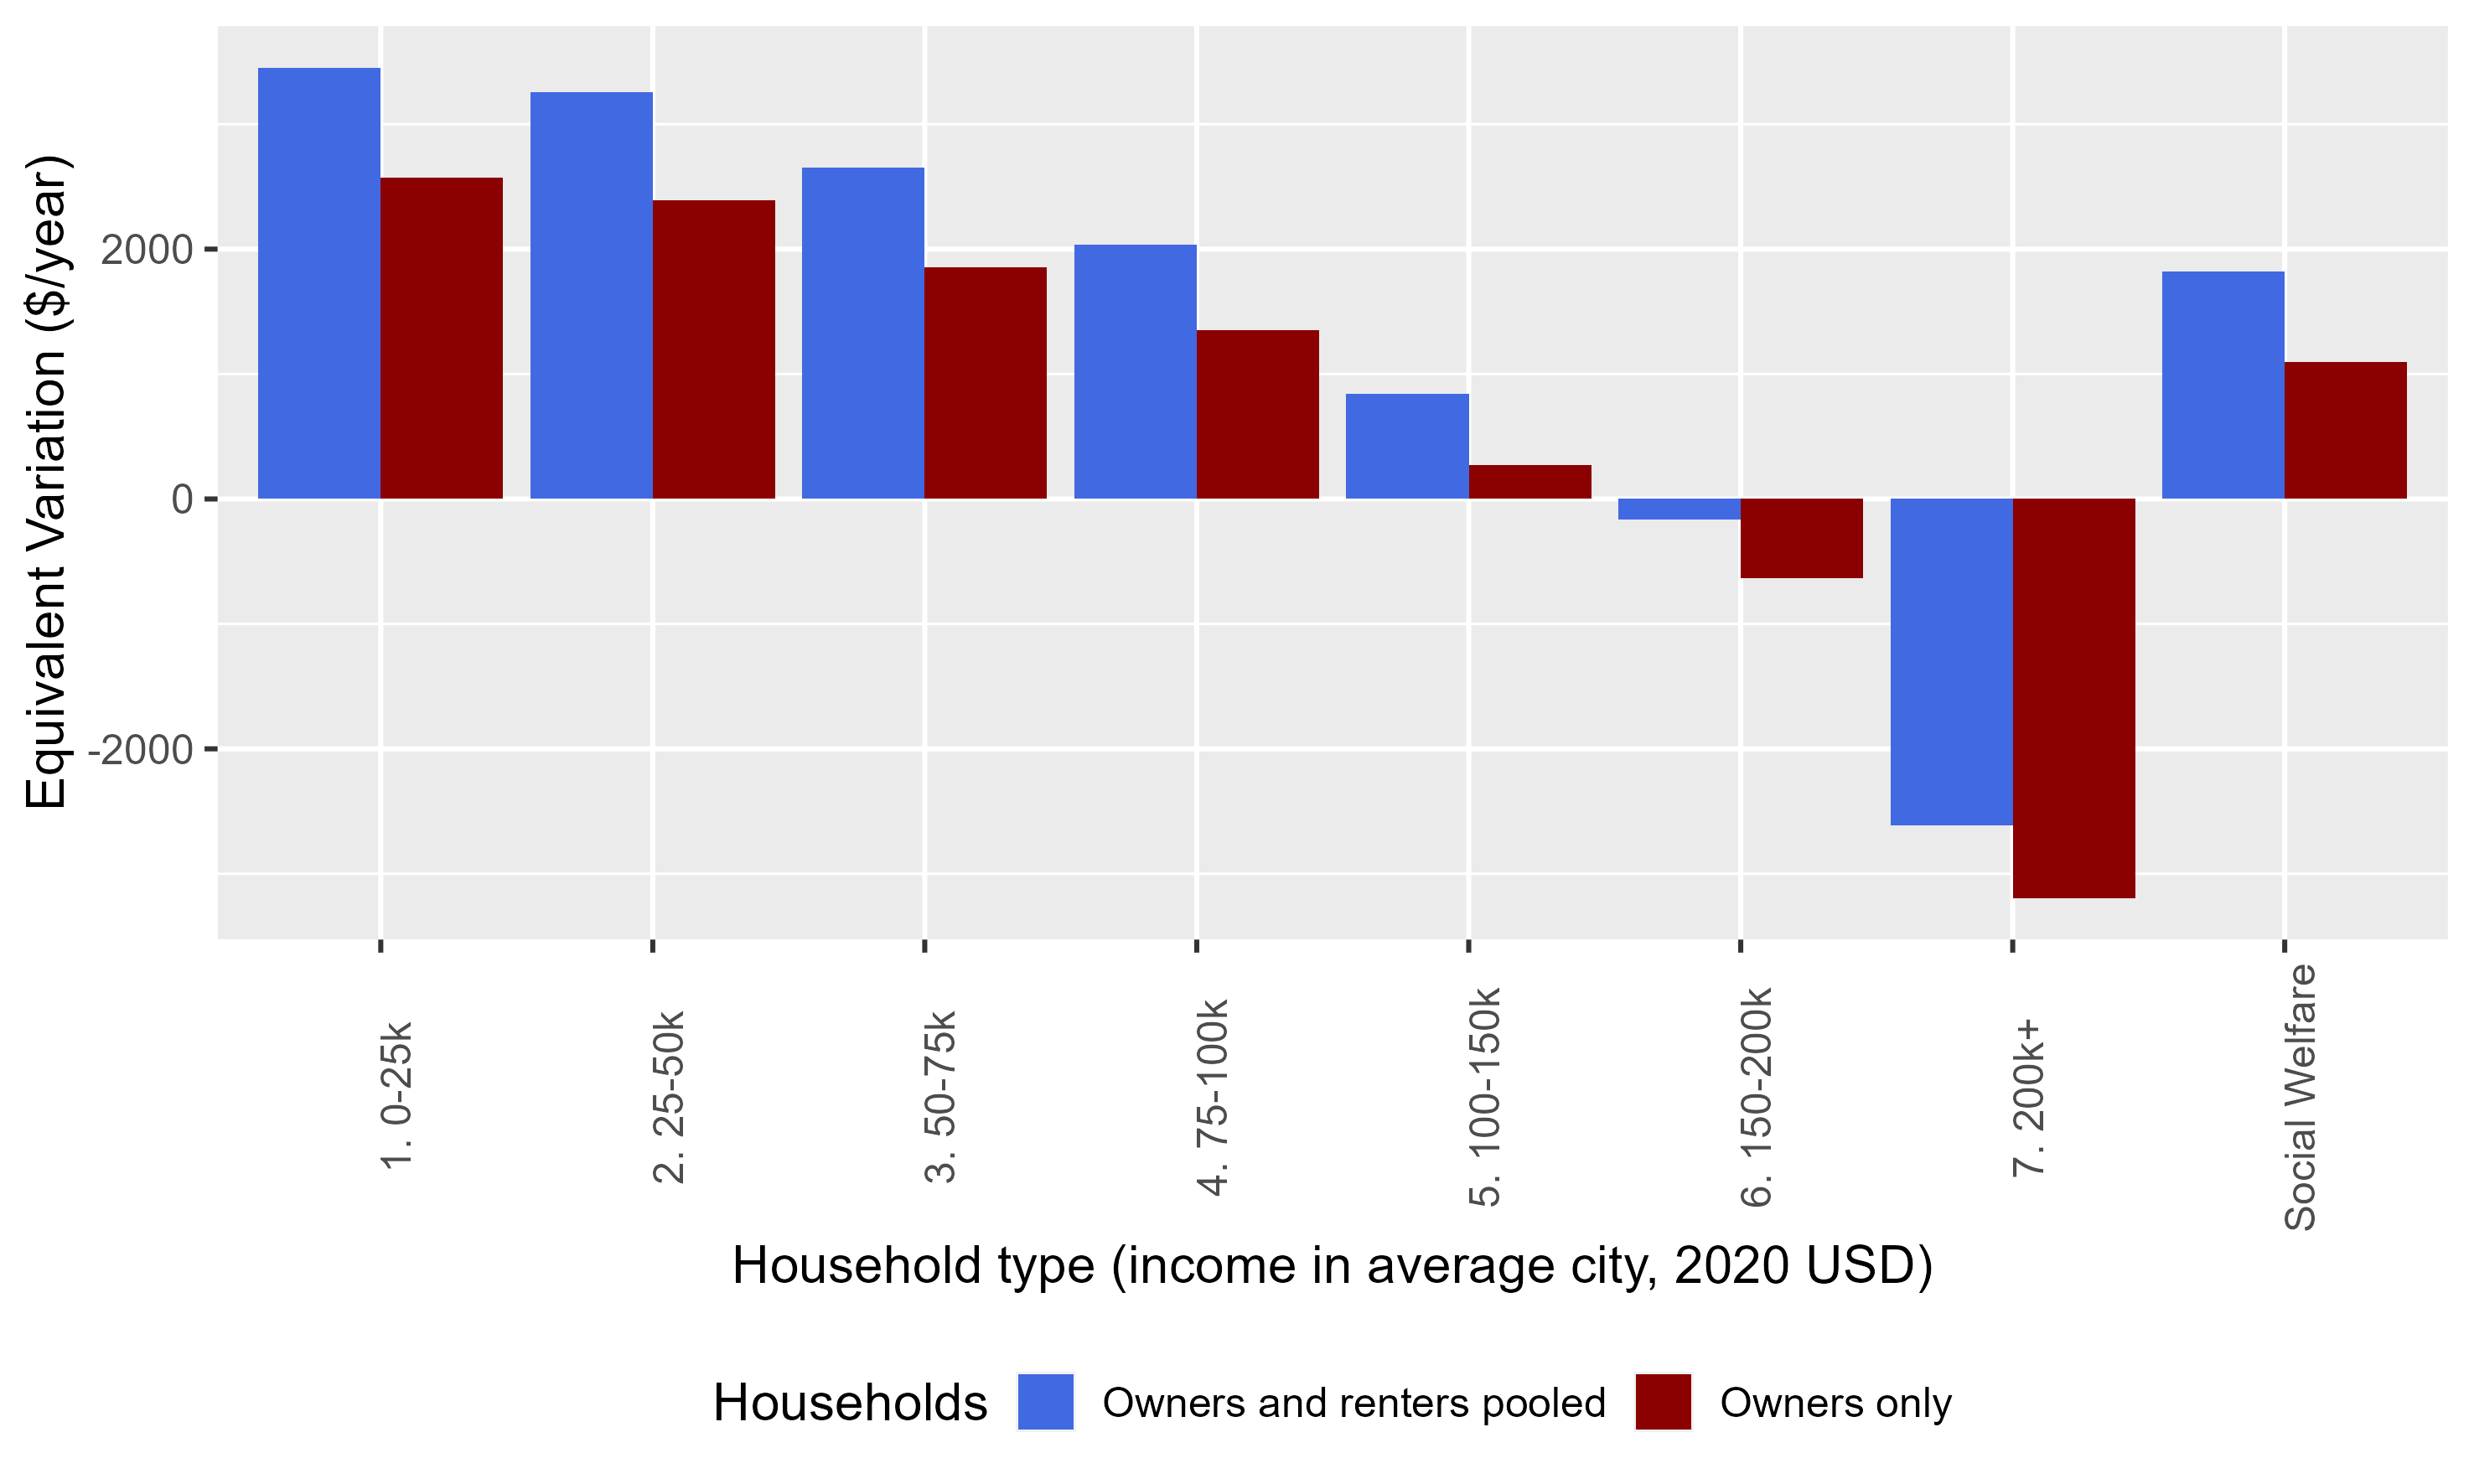
\includegraphics[width=\textwidth]{WelfarePooled_nopercent.png}}
		\end{center}
		\caption*{Welfare is measured as the equivalent variation. Higher values mean higher welfare gains. Social welfare is the population weighted average of welfare by type. Results incorporate capital losses for homeowners by income type, using a procedure outlined in Appendix \ref{Appendix:RenterLandownerWelfare}. Results include equilibrium adjustments to neighborhood amenity value as in the baseline counterfactual. Renters and homeowners are pooled by type using a population-weighted average of welfare changes.}
	\end{figure}
	
	
	\begin{figure}[htbp!]
		
		\caption{Income-Density Gradients in baseline and counterfactual after complete deregulation.}\label{figure:gentrification_alternate}
		\makebox[\textwidth]{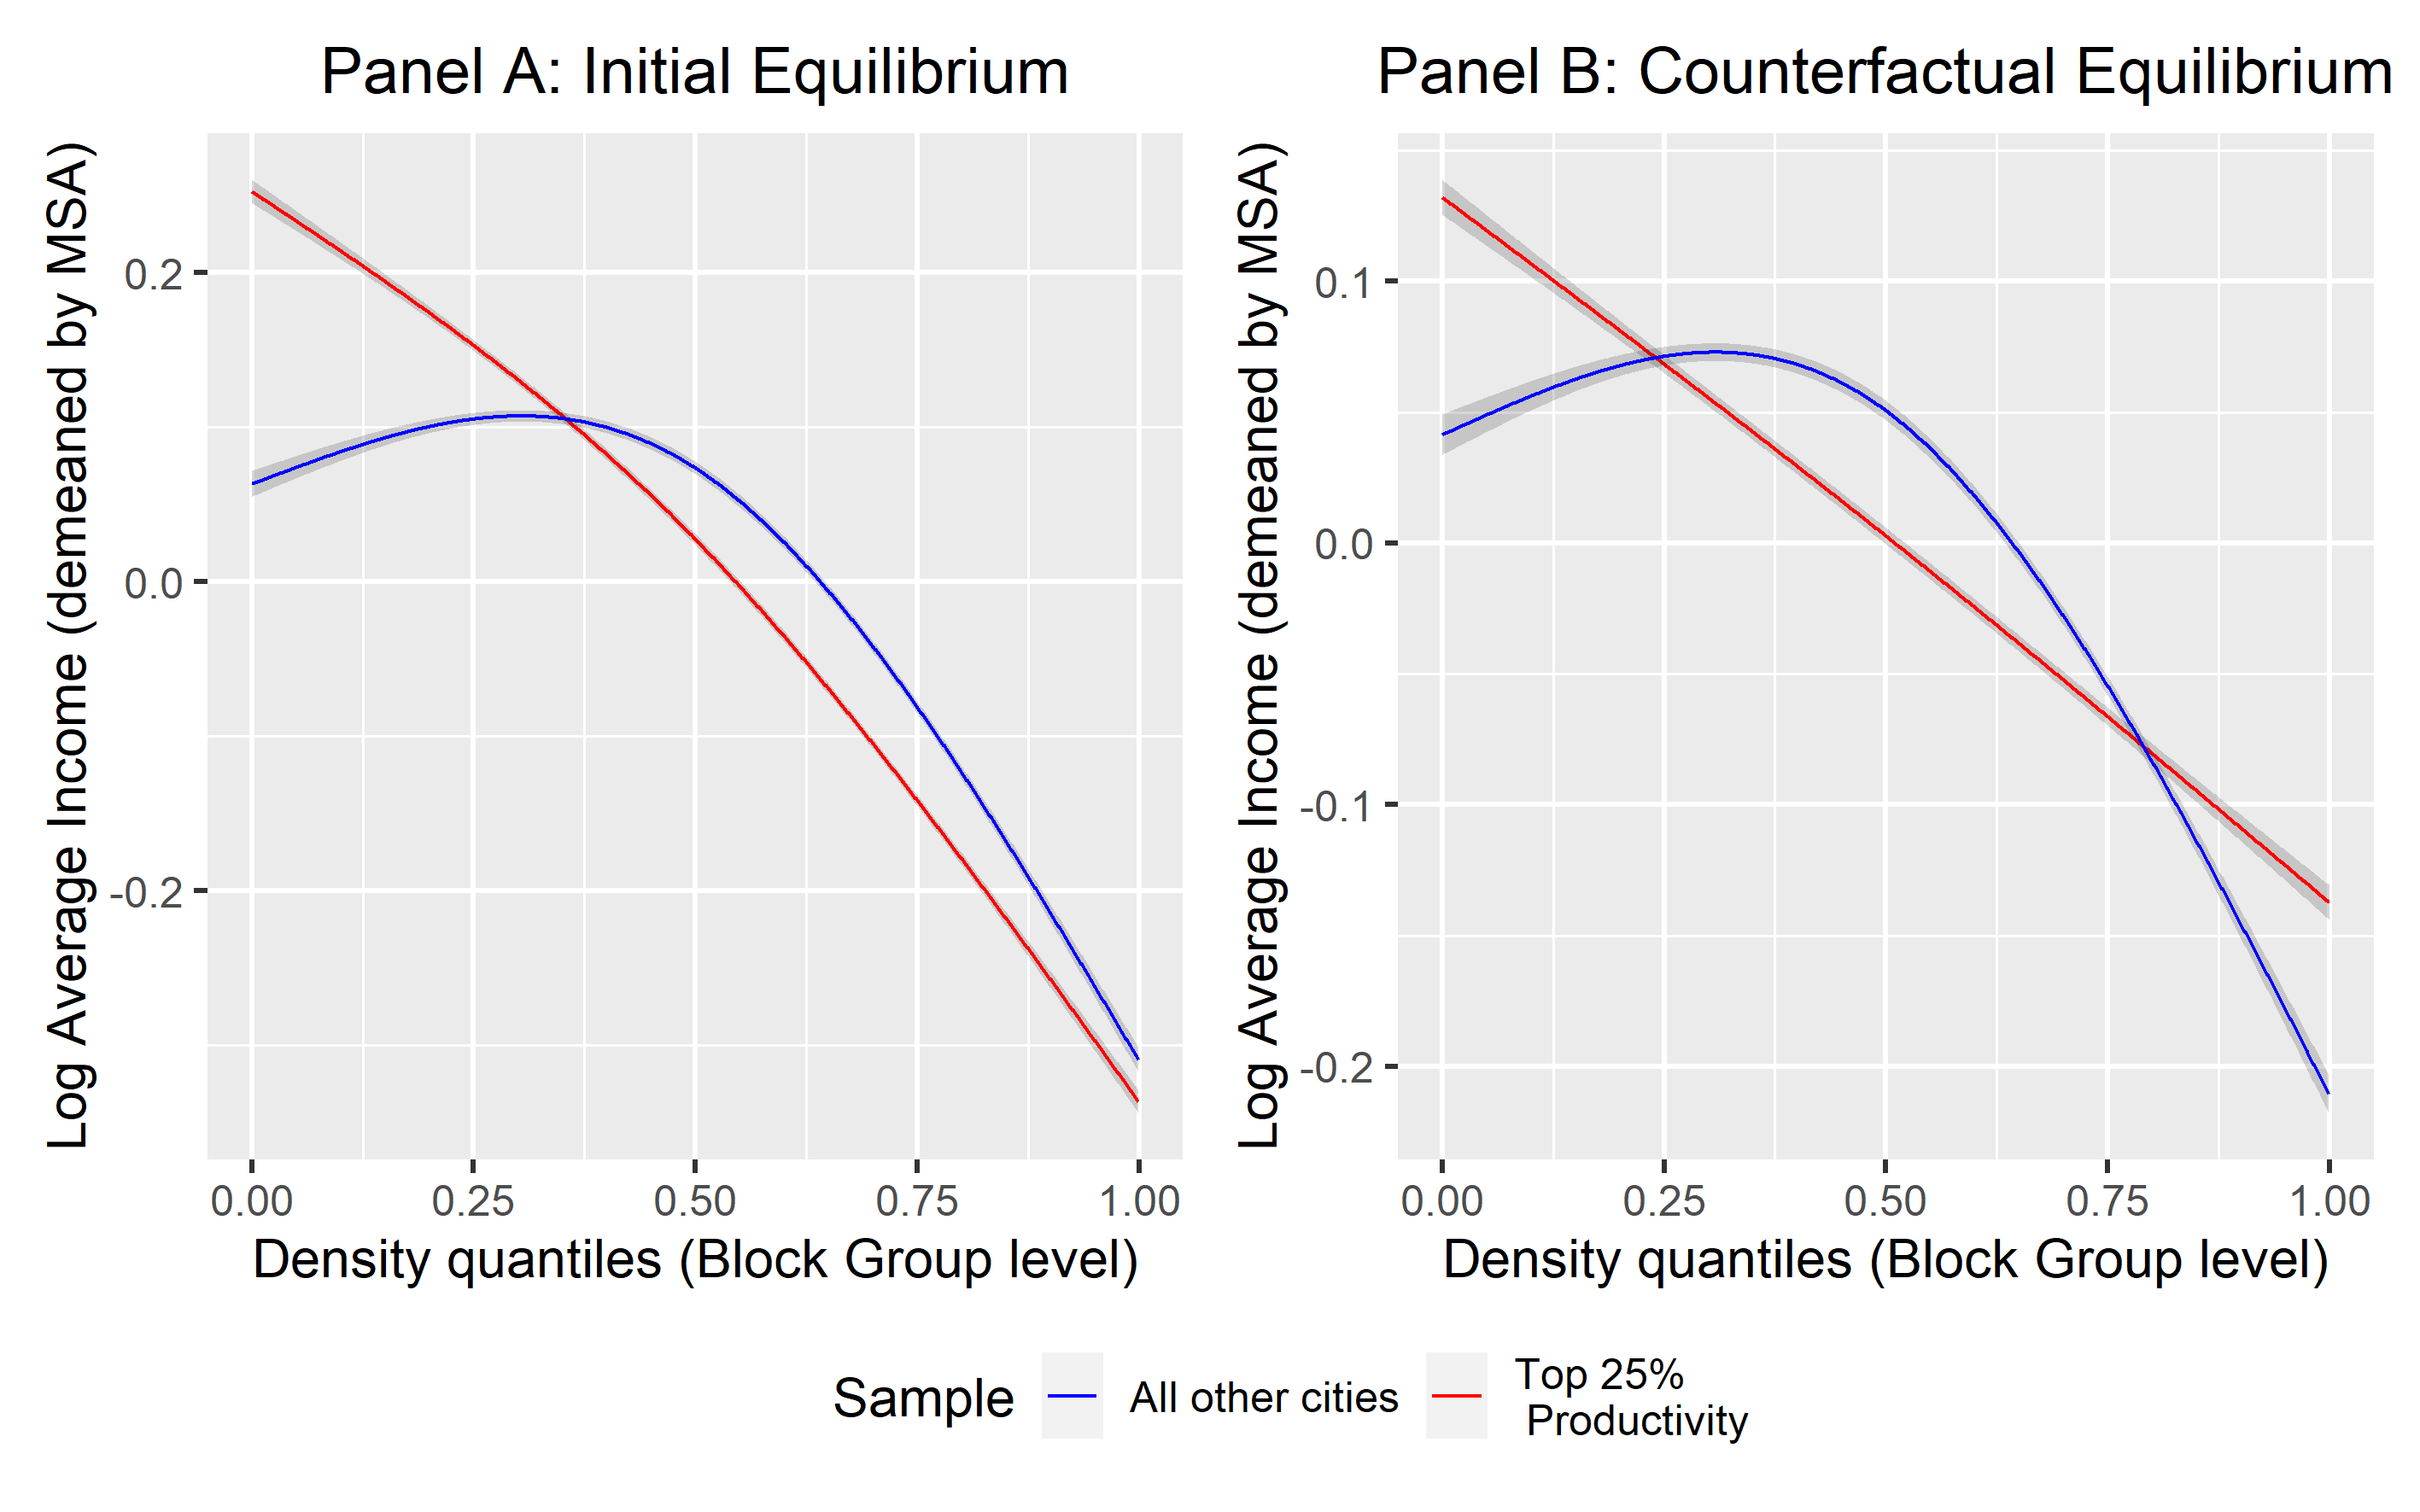
\includegraphics[width=\textwidth]{IncomeDensityGradCtfl_alternate.png}}
		
		\caption*{Panel B corresponds to the same estimates of Panel A of Figure \ref{FIncomeDens}. Panel A compares the income density gradient across "superstar" sample cities and "non-superstar" cities that is generated in an equilibrium without minimum lot sizes. The gentrification of high density neighborhoods is apparent. Differences in the income density gradient across samples disappear when transitioning from the initial equilibrium to the counterfactual equilibrium.}
		
	\end{figure}
	
	
	\begin{landscape}
			\begin{table}[h]
			
			\centering
			\caption{Effects of unilaterally halving minimum lot sizes in select cities.}\label{table:ctfl_dereg_in_cities}
			\makebox[\textwidth]{	 \centering \renewcommand*{\arraystretch}{1.4}
\begin{tabular}{lllllllllll}
\hline
\hline
City & Superstar? & Endogenous Amenities & 0-25k & 25-50k & 50-75k & 75-100k & 100-150k & 150-200k & 200k+ & Land Values \\ 
\hline
San Francisco & Yes & Yes & 0.13 & 0.16 & 0.14 & 0.11 & 0.08 & 0.04 & -0.02 & -1.6 \\ 
 &  & No & 0.23 & 0.25 & 0.27 & 0.19 & 0.13 & 0.08 & 0.02 & 11.81 \\ 
Washington & Yes & Yes & 0.39 & 0.24 & 0.16 & 0.12 & 0.07 & 0.03 & -0.03 & -10.08 \\ 
 &  & No & 0.49 & 0.29 & 0.21 & 0.16 & 0.12 & 0.08 & 0.03 & -0.51 \\ 
Denver & Yes & Yes & 0.26 & 0.21 & 0.13 & 0.09 & 0.06 & 0.03 & 0 & -14.71 \\ 
 &  & No & 0.32 & 0.25 & 0.17 & 0.12 & 0.09 & 0.05 & 0.02 & -1.76 \\ 
Los Angeles & Yes & Yes & 0.37 & 0.5 & 0.34 & 0.32 & 0.2 & 0.09 & 0 & -0.31 \\ 
 &  & No & 0.61 & 0.73 & 0.58 & 0.52 & 0.32 & 0.17 & 0.05 & 14.74 \\ 
New York City & Yes & Yes & 1.09 & 0.46 & 0.27 & 0.19 & 0.1 & 0.05 & -0.02 & -3.67 \\ 
 &  & No & 1.47 & 0.62 & 0.36 & 0.24 & 0.16 & 0.1 & 0.05 & 0.1 \\ 
Tampa Bay & No & Yes & 0.31 & 0.13 & 0.06 & 0.04 & 0.02 & 0.01 & 0.01 & -14.65 \\ 
 &  & No & 0.35 & 0.15 & 0.07 & 0.04 & 0.03 & 0.02 & 0.01 & -8.93 \\ 
San Antonio & No & Yes & 0.22 & 0.09 & 0.05 & 0.03 & 0.02 & 0.01 & 0.01 & -17.31 \\ 
 &  & No & 0.24 & 0.09 & 0.05 & 0.03 & 0.02 & 0.01 & 0.01 & -11.12 \\ 
Rochester & No & Yes & 0.02 & 0.01 & 0 & 0 & 0 & 0 & 0 & -3.95 \\ 
 &  & No & 0.02 & 0.01 & 0 & 0 & 0 & 0 & 0 & -2.23 \\ 
Tucson & No & Yes & 0.08 & 0.04 & 0.02 & 0.01 & 0.01 & 0 & 0 & -15.51 \\ 
 &  & No & 0.1 & 0.05 & 0.03 & 0.02 & 0.01 & 0.01 & 0 & -7.03 \\ 
St. Louis & No & Yes & 0.11 & 0.05 & 0.03 & 0.02 & 0.01 & 0 & 0 & -10.06 \\ 
 &  & No & 0.12 & 0.06 & 0.03 & 0.02 & 0.01 & 0.01 & 0.01 & -4.02\\ 
\hline
\hline
\multicolumn{11}{l}{}\\ 
\end{tabular}


 }
			
			\caption*{Changes in renter welfare are measured using the equivalent variation measure and conditional on living in the respective city post deregulation (expressed as \% of income). Because of the assumption of Gumbel preference shocks, the average utility of households that choose these cities is the same as an average household nationally. Changes in land values are expressed in \% of initial land value within the deregulating city.}
			
		\end{table}
	\end{landscape}
	
	
	
	%%%%%%%%%%%%%%%%%%%%%%%%%%%% OPTIMAL POLICY
		\begin{figure}[htbp!]
		
		\caption{Shapely decomposition of welfare effects from permuted policy}\label{figure:WelfareDecomp_optPolicy}
		\makebox[\textwidth]{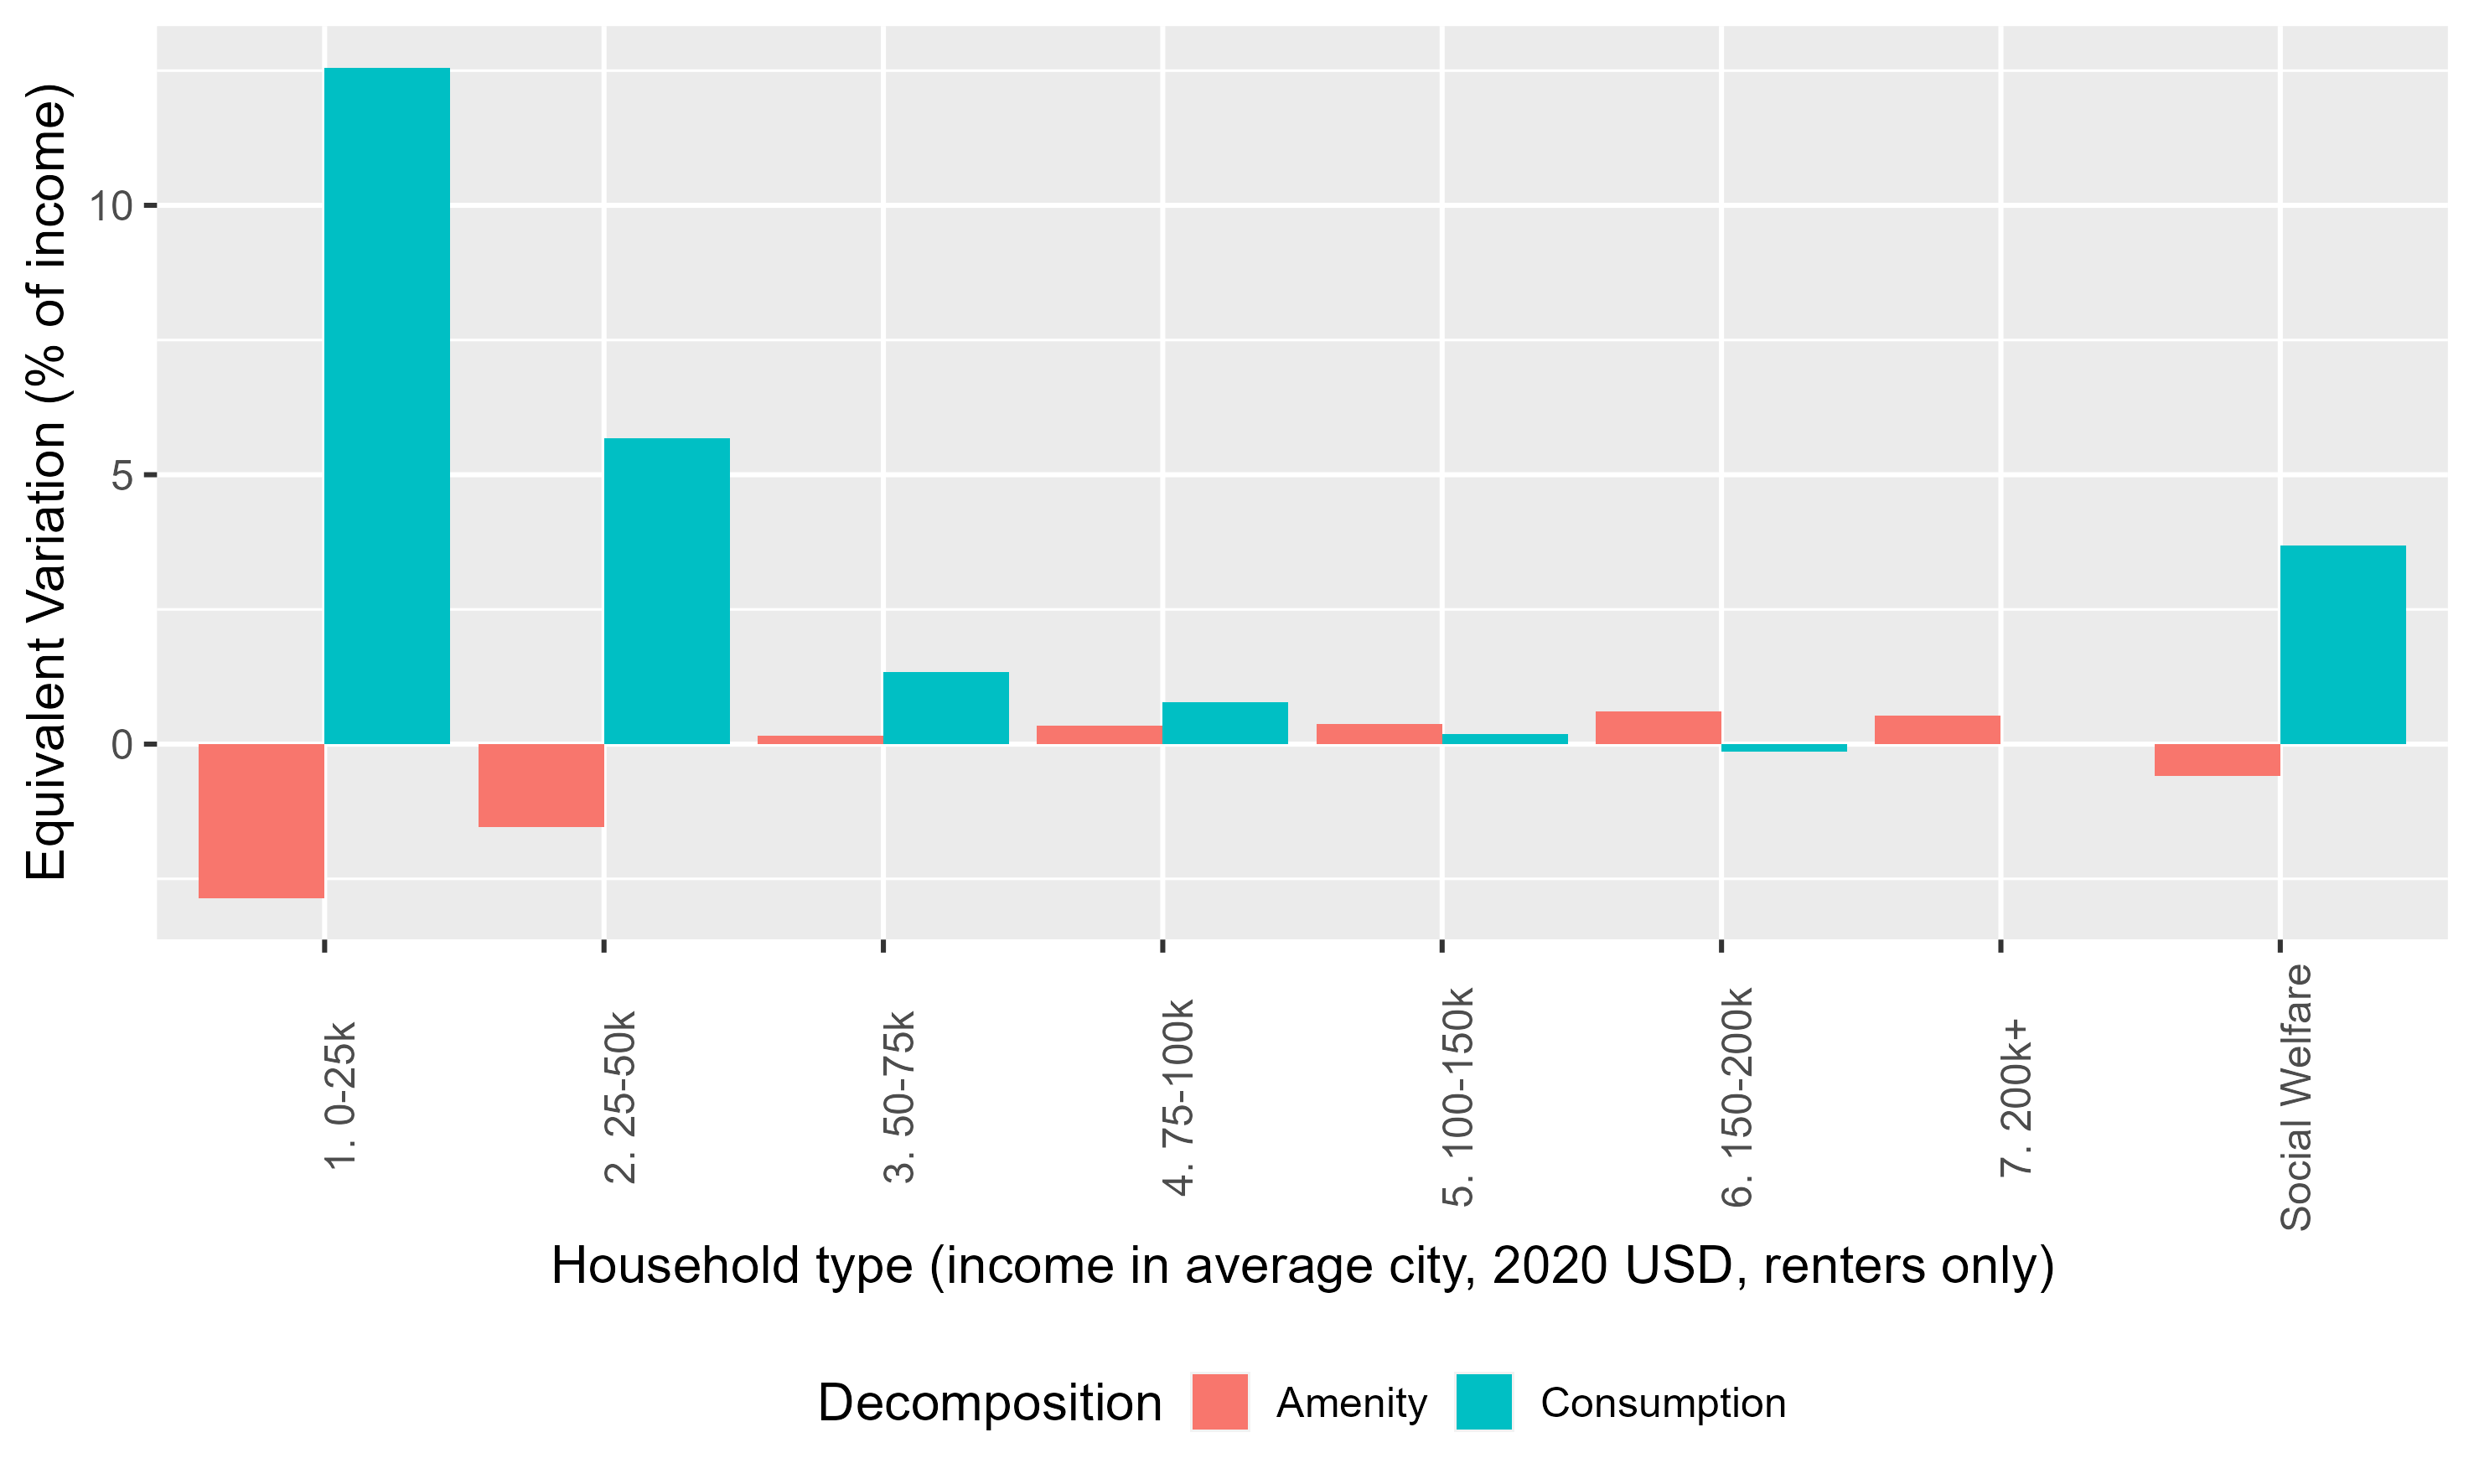
\includegraphics[width=\textwidth]{WelfareDecomp_optPolicy.png}}
		
		\caption*{Welfare is measured as the equivalent variation as a percentage of baseline income. Higher values mean higher welfare gains. Social welfare is the population weighted average of welfare by type. "Amenity" and "Consumption" components are constructed using Shapely values, with a procedure outlined in Appendix \ref{Appendix:ShapeDecompDefn}. The sum of components add to the equivalent variation associated with the policy that permutes regulation to target rich neighborhoods.}
		
	\end{figure}
	
	
	%%%%%%%%%%%%%%
	
	\begin{figure}[htbp!]
		
		\caption{Shapely decomposition of welfare effects from permuted policy, in \$}\label{figure:WelfareDecomp_optPolicy_nopercent}
		\makebox[\textwidth]{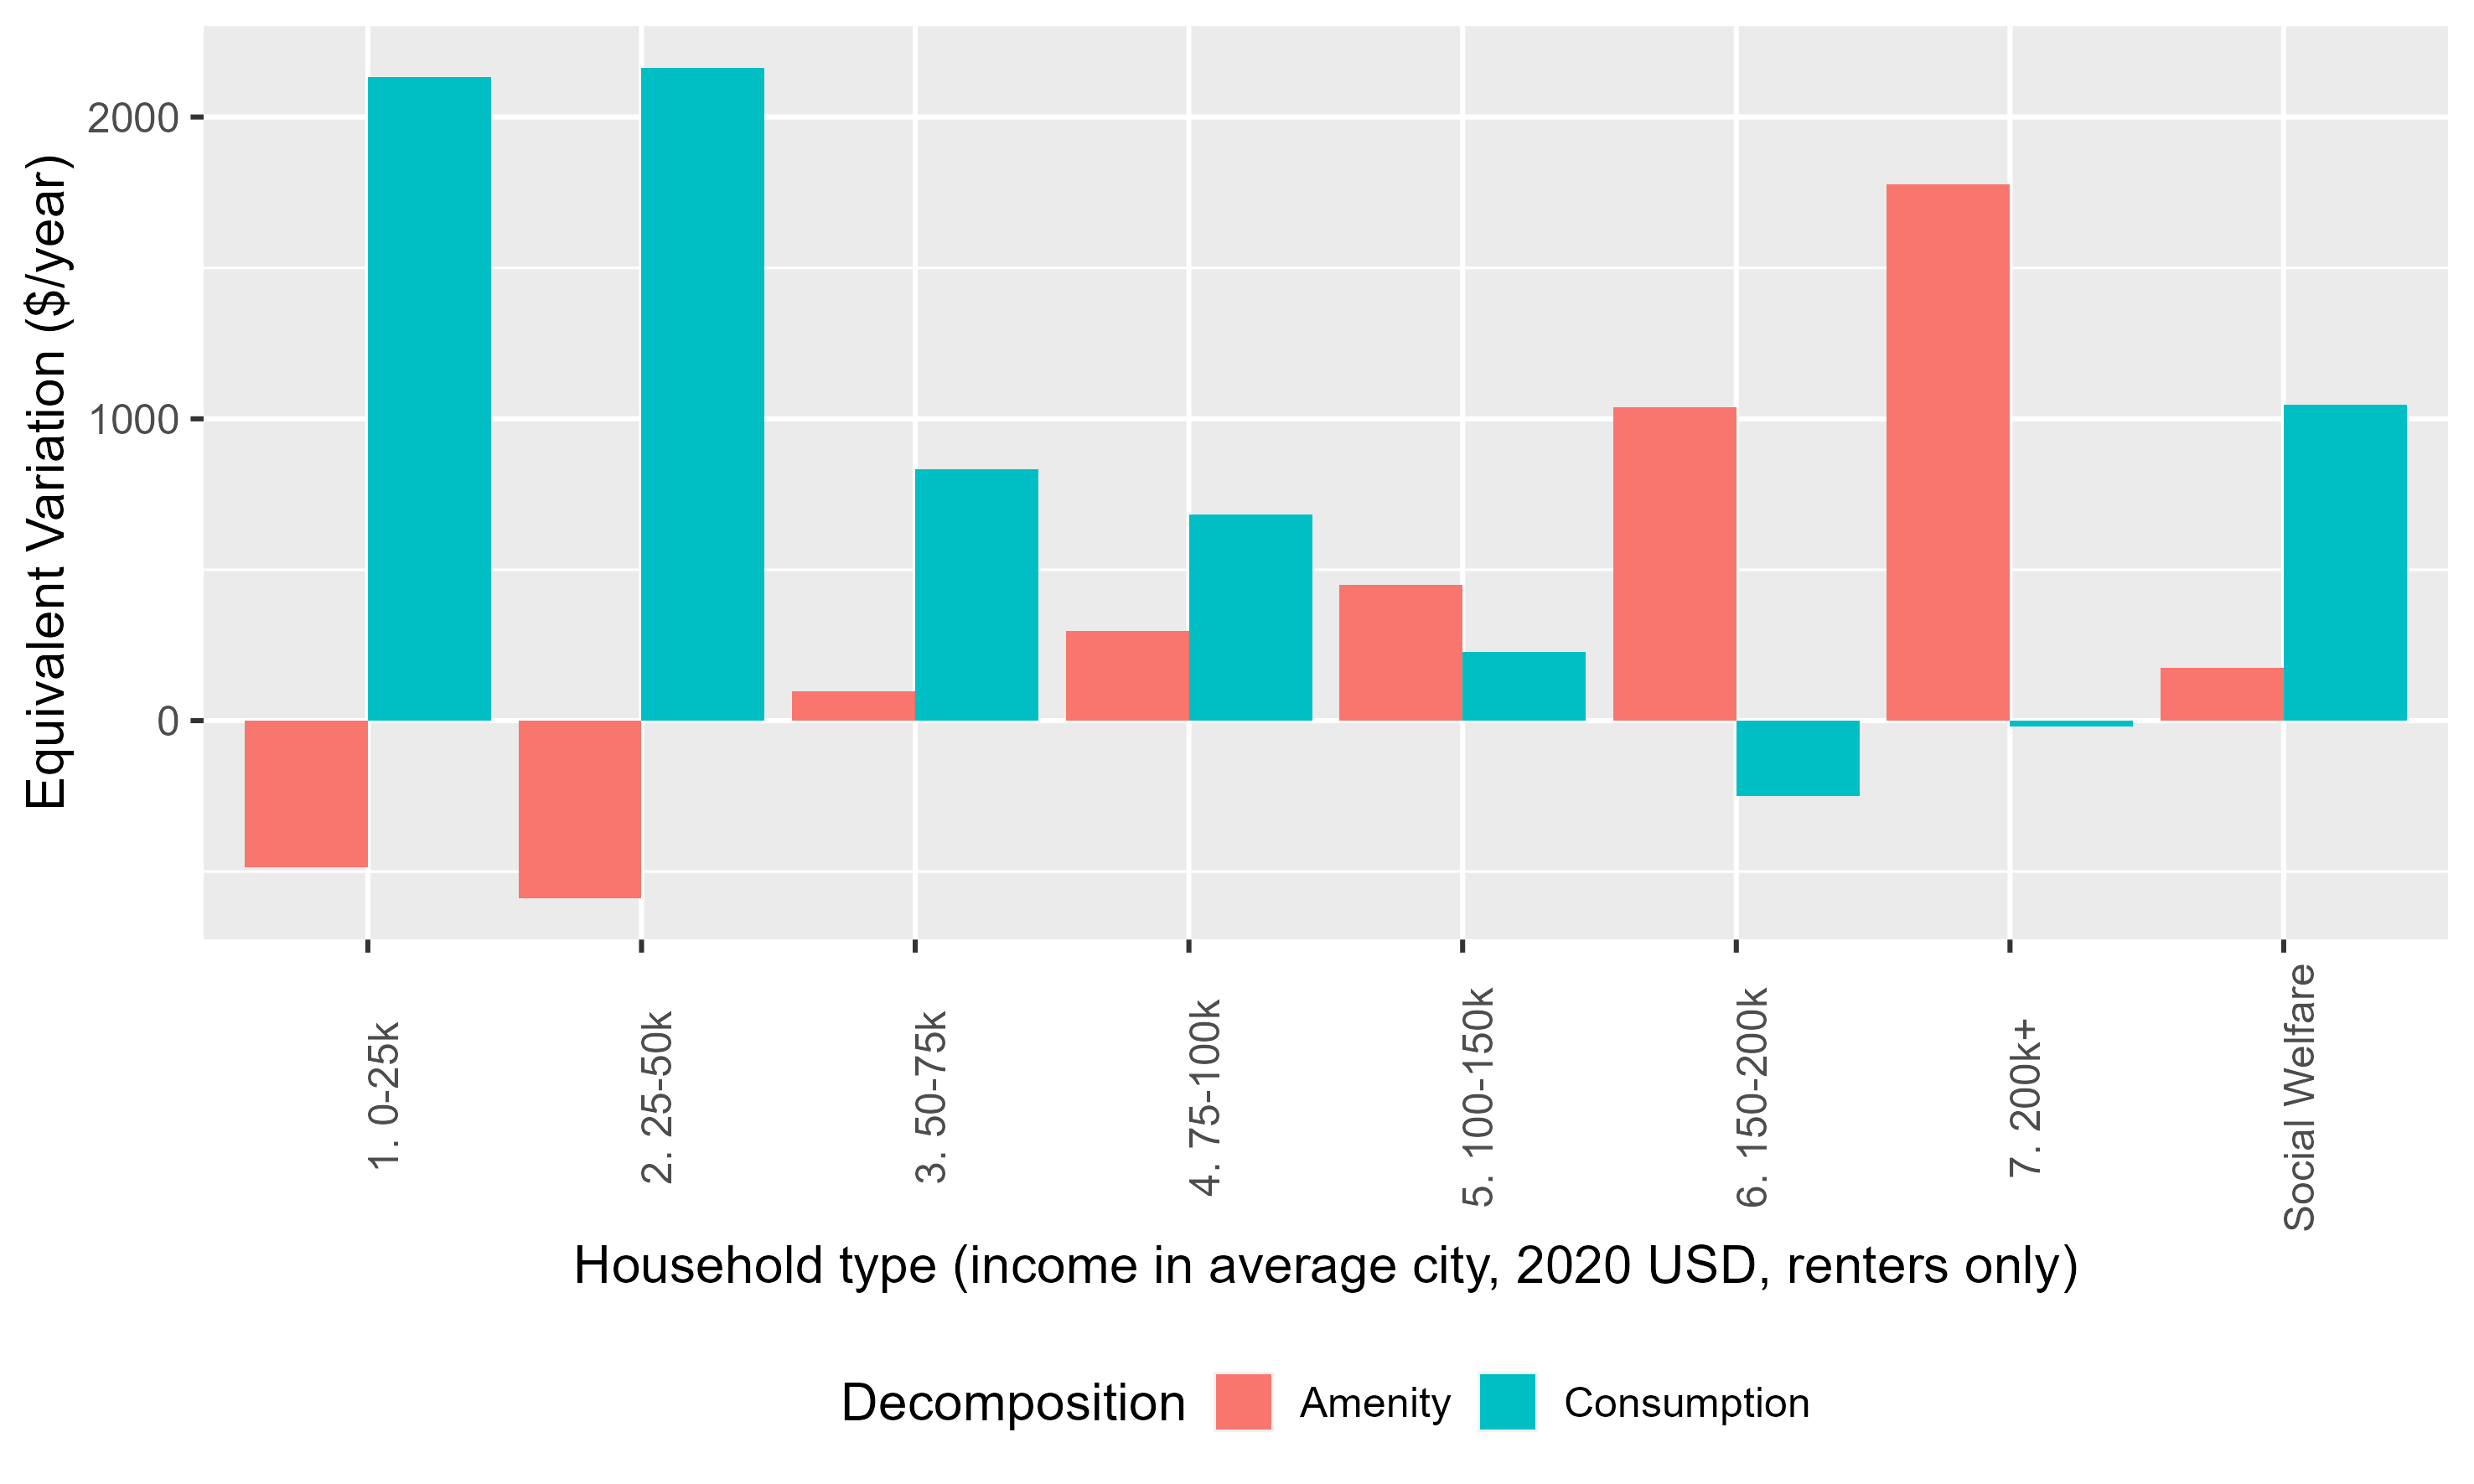
\includegraphics[width=\textwidth]{WelfareDecomp_nopercent_optPolicy.png}}
		
		\caption*{Welfare is measured as the equivalent variation. Higher values mean higher welfare gains. Social welfare is the population weighted average of welfare by type. "Amenity" and "Consumption" components are constructed using Shapely values, with a procedure outlined in Appendix \ref{Appendix:ShapeDecompDefn}. The sum of components add to the equivalent variation associated with the policy that permutes regulation to target rich neighborhoods.}
		
	\end{figure}
	
	
	\begin{landscape}
	\begin{figure}[htbp!]
		\begin{center}
			\caption{City income sorting after permuting regulation.}\label{figure:city_inc_sorting_optPolicy}
			\makebox{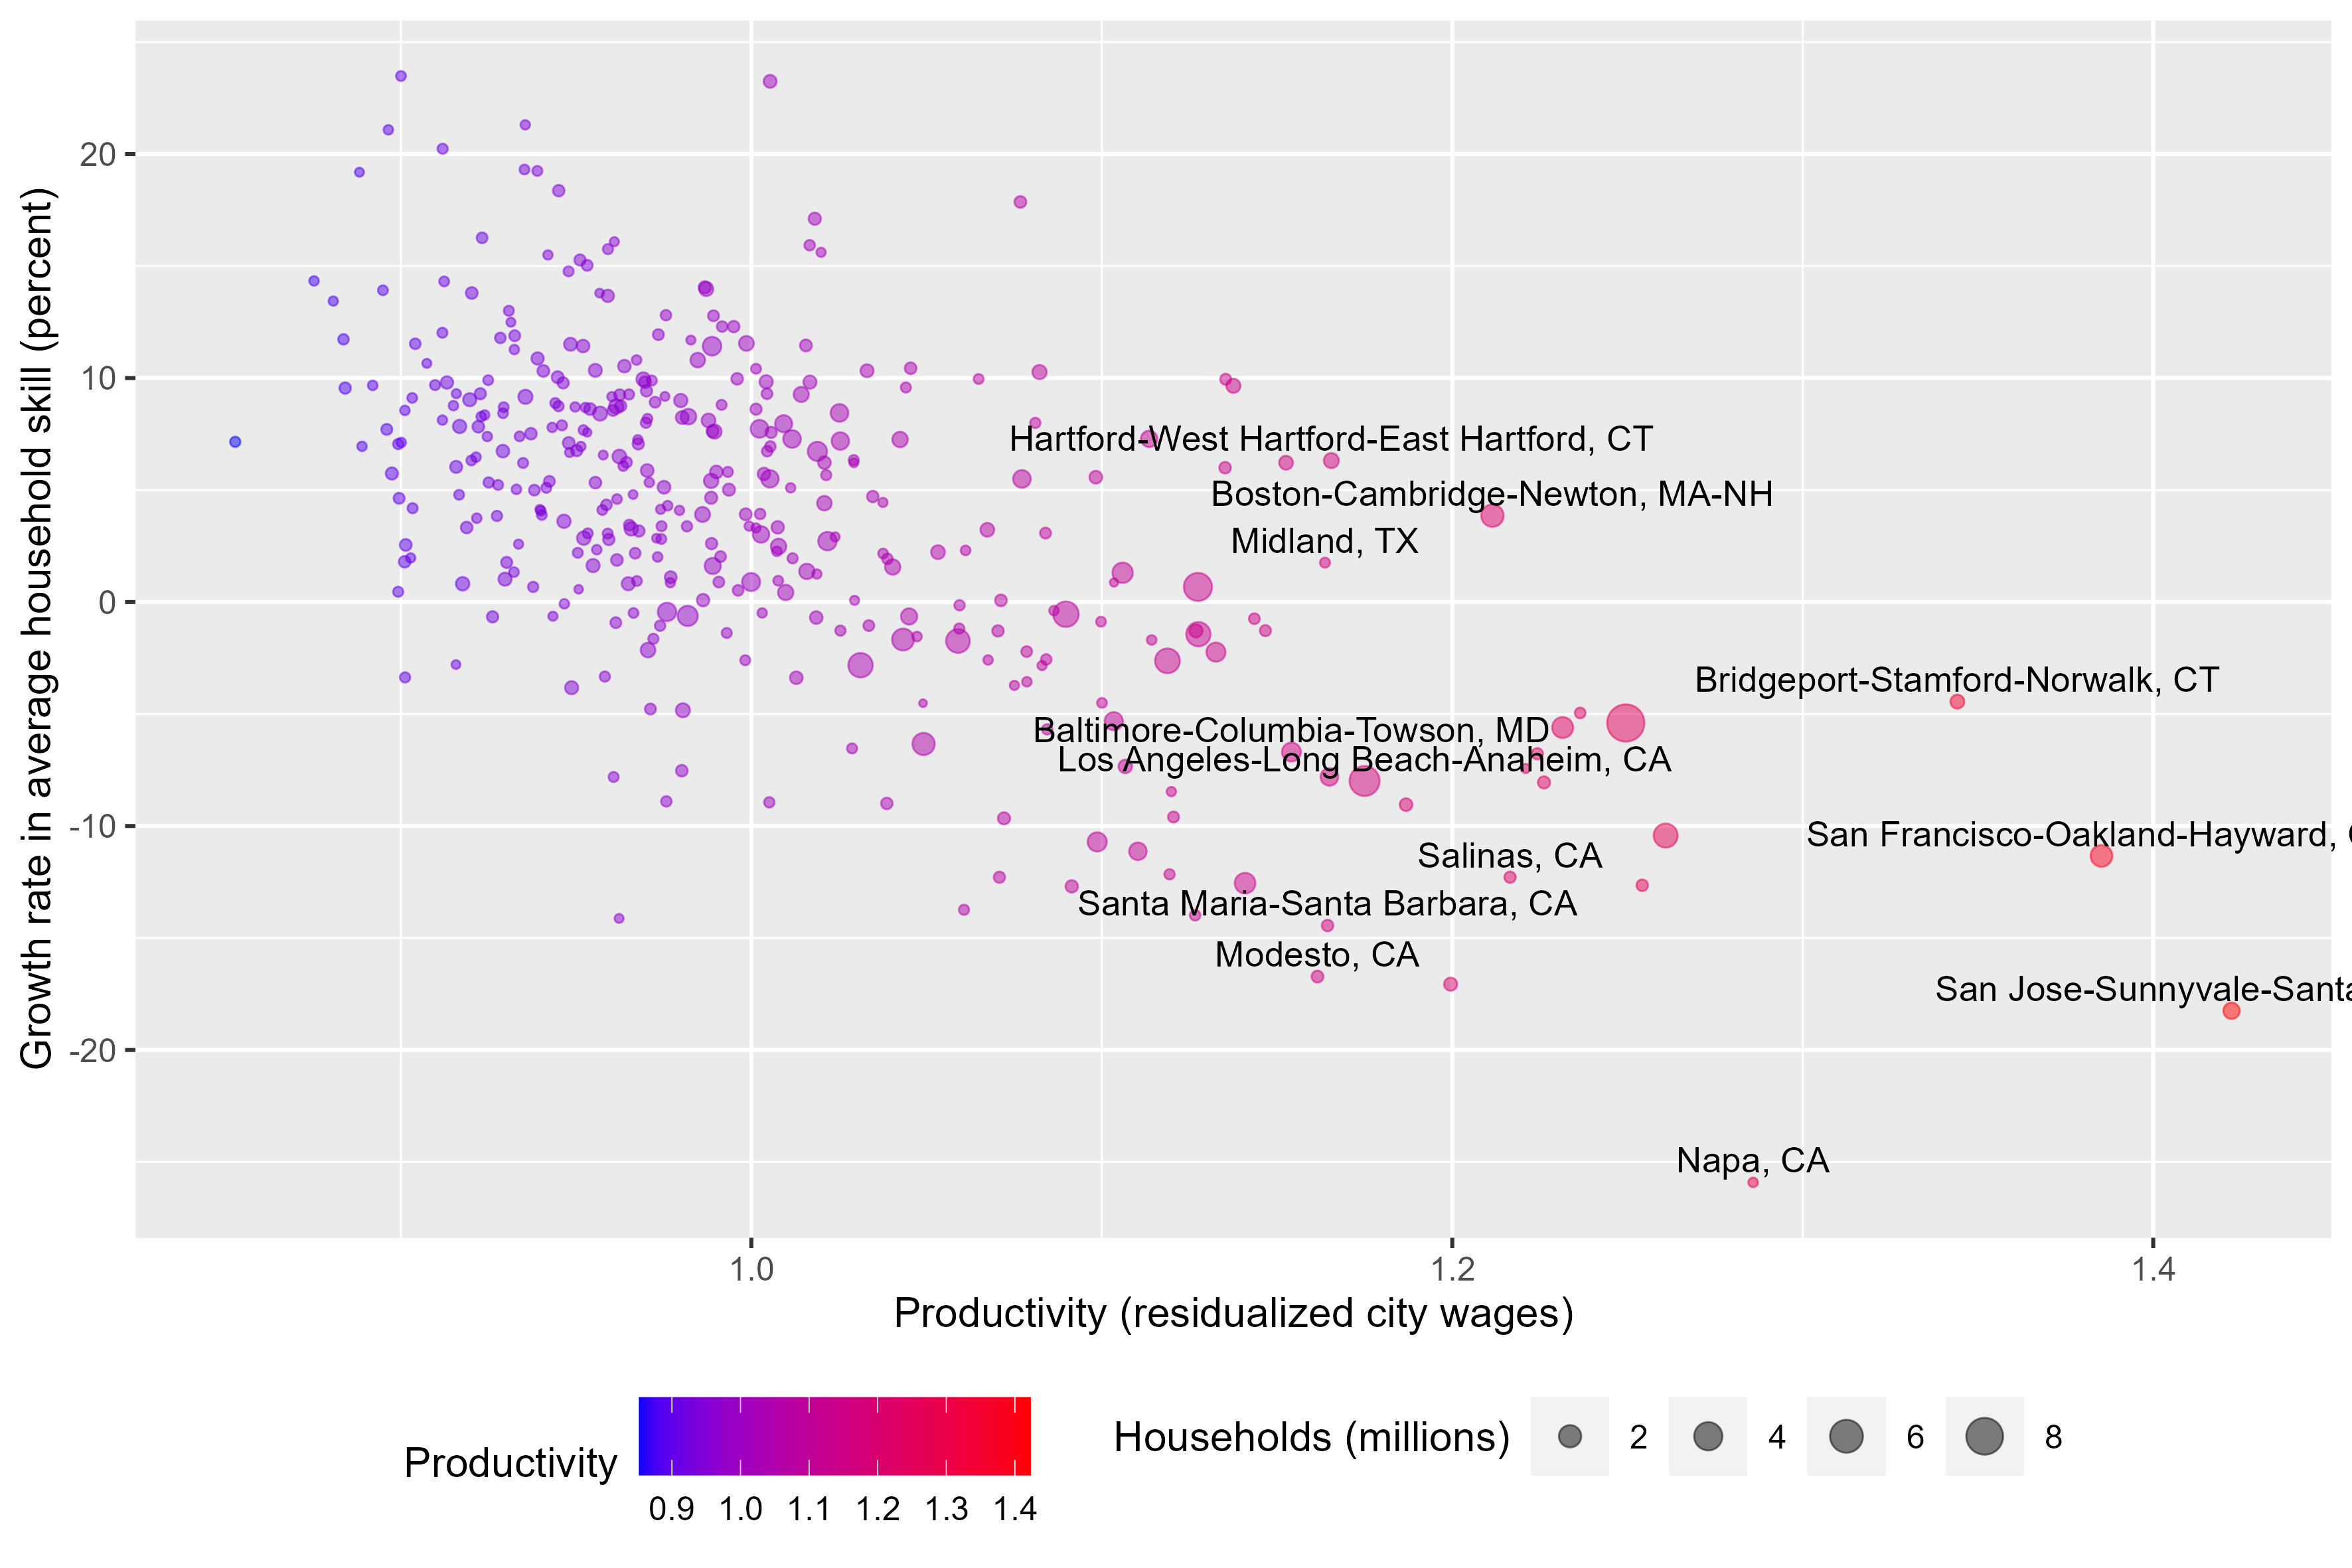
\includegraphics[width = 0.9\linewidth, height = \textheight]{IncomeSortingMovement_optPolicy.png}}
			
			\caption*{The $y$ axis is defined as the change in the average income that a household could earn in an average city from baseline to counterfactual. The $x$ axis measures city productivity (residualized wages from the data). The permuted policy disproportionately deregulates productive cities, suggesting that the amenity valuation of productive cities for high skill people is not high enough to justify regulation. }
		\end{center}
	\end{figure}
\end{landscape}
	
	
	
	
	
	\begin{figure}[htbp!]
	
	\caption{ \\ Gentrification in superstar cities after permuting regulation.}\label{figure:gentrification_optPolicy}
	\makebox[\textwidth]{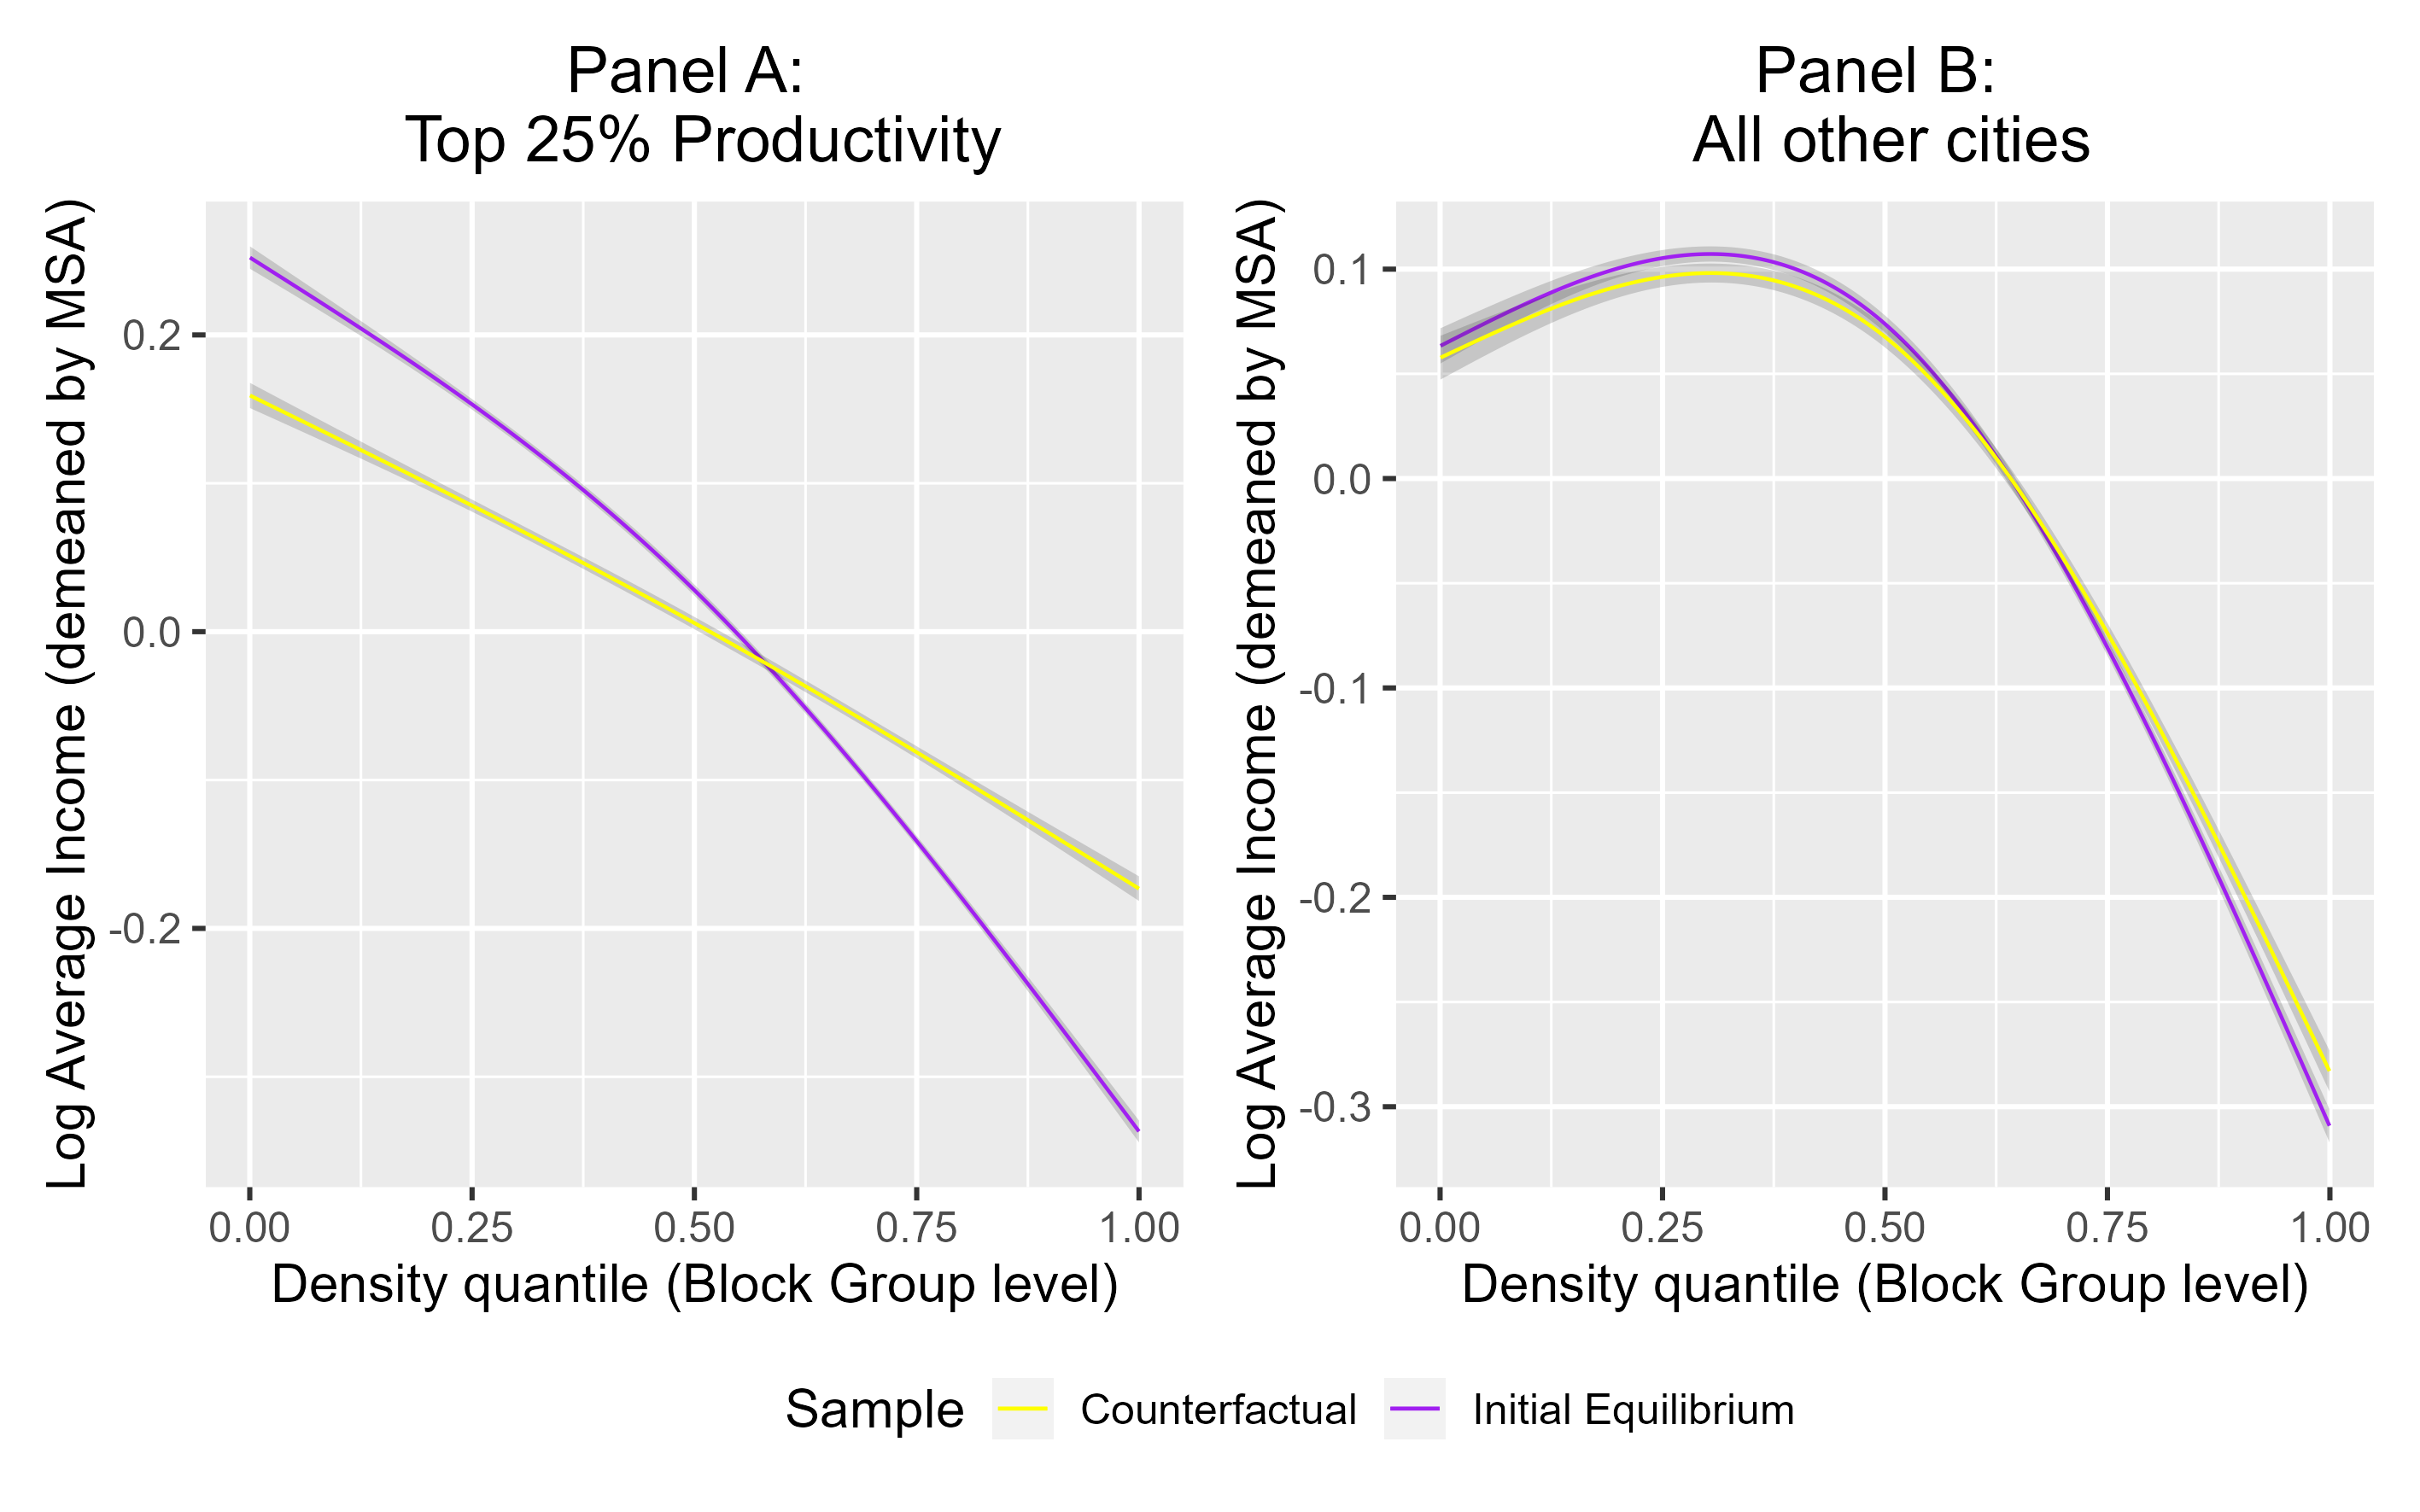
\includegraphics[width=\textwidth]{IncomeDensityGradCtfl_optPolicy.png}}
	
	\caption*{For each panel, demeaned log average income at the neighborhood level is regressed against the observed density ranking of neighborhoods at baseline. The purple regression uses data from the baseline equilibrium that matches data, as in Figure \ref{FIncomeDens}. The yellow regression uses data generated from the counterfactual where regulation is permuted to target rich neighborhoods based on the high-skill amenity score. Each panel corresponds to "superstar" sample cities (Top $25 \%$) and "non-superstar" sample cities (Bottom $75 \%$), as in Figure \ref{FIncomeDens}. This policy change suggests that low-skill households somewhat value low density neighborhoods in productive cities, but regulation otherwise makes them too exclusive.}
	
\end{figure}

	
	
	
\end{document}